\documentclass[svgnames,table]{beamer}
\usepackage{hhline}
\usepackage{etoolbox}
\usepackage{tikz}
\usepackage{mathtools}
%\usepackage{/usr/lib64/R/share/texmf/Sweave}
\mode<presentation>







\usetheme{Frankfurt}%
\usecolortheme{seagull}
\logo{
\includegraphics[height=.25in]{img/clarksonGreen}}

\definecolor{garnet}{RGB}{136,0,0}
%\definecolor{clarksonGreen}{RGB}{0,71,28}
\definecolor{clarksonGreen}{RGB}{0,52,21}
\setbeamercolor{palette primary}{fg=clarksonGreen,bg=white}
\setbeamercolor{palette secondary}{fg=clarksonGreen,bg=white}
\setbeamercolor{palette tertiary}{fg=clarksonGreen,bg=white}
\setbeamercolor{palette quaternary}{bg=clarksonGreen,fg=white}
\setbeamercolor{block title}{fg=black,bg=black!15}
\setbeamercolor{block body}{fg=black,bg=black!10}
\setbeamercolor{titlelike}{bg=clarksonGreen,fg=white} % parent=palette quaternary}

\newcommand{\half}{\mbox{$\frac{1}{2}$}}
\newcommand{\deltat}{\mbox{$\triangle t$}}
\newcommand{\deltax}{\mbox{$\triangle x$}}
\newcommand{\deltay}{\mbox{$\triangle y$}}

\newcommand{\deriv}[2]{\frac{d}{d#2}#1}
\newcommand{\derivTwo}[2]{\frac{d^2}{d#2^2}#1}

\newcommand{\lp}{\left(}
\newcommand{\rp}{\right)}


\newtoggle{clicker}
\toggletrue{clicker}
%\togglefalse{clicker}


% To display a lecture uncomment out the "includeonly" line below to
% match the name of the file. You do not have to do anything with the
% lecture line below and can leave it commented out. It is in place
% because at one time we had multiple lectures within a file, but that
% has been changed.


% %%%%%%%%%%%%%%%%%%%%%%%%%%%%%%%%%%%%%%%%%%%%%%%%%%%%%%%%%%%%
%\includeonly{introduction}
% %%%%%%%%%%%%%%%%%%%%%%%%%%%%%%%%%%%%%%%%%%%%%%%%%%%%%%%%%%%%
%\includeonly{probabilityI}
%\includeonly{probabilityII}
%\includeonly{conditionalProb}
%%\includeonly{conditionalProbII}
%\includeonly{counting}
% %%%%%%%%%%%%%%%%%%%%%%%%%%%%%%%%%%%%%%%%%%%%%%%%%%%%%%%%%%%%
%\includeonly{discreteRV}
%\includeonly{binomial}
%\includeonly{normal}
%\includeonly{generalNormal}
%\includeonly{normalApplications}
% %%%%%%%%%%%%%%%%%%%%%%%%%%%%%%%%%%%%%%%%%%%%%%%%%%%%%%%%%%%%
%\includeonly{qualitative}
%\includeonly{quantitative}
%\includeonly{position}
%%\includeonly{groupedData}
%\includeonly{quantiles}
%\includeonly{normality}
%\includeonly{approxBinomial}
% %%%%%%%%%%%%%%%%%%%%%%%%%%%%%%%%%%%%%%%%%%%%%%%%%%%%%%%%%%%%
%\includeonly{sampleDist}
%\includeonly{sampleProportions}
%\includeonly{confInterval}
%\includeonly{t-distribution}
%\includeonly{proportionConfInterval}
\includeonly{confIntervalsDecisions}
%\includeonly{hypTest}
%\includeonly{hypTestMean}
%\includeonly{hypTestTDist}
%\includeonly{propHypTest}
%\includeonly{hypTestDecisions}
% %%%%%%%%%%%%%%%%%%%%%%%%%%%%%%%%%%%%%%%%%%%%%%%%%%%%%%%%%%%%
%\includeonly{bivariate}
%\includeonly{regression}
%\includeonly{correlation}
%\includeonly{regressionSignificance}
%\includeonly{predictionIntervals}



\begin{document}

\author{Kelly Black}
\institute{Clarkson University}




\lecture{Introduction}{Introduction}
\section{Introduction}

\title{Statistics}
\subtitle{Introduction To Statistics and Course Information}

%\author{Kelly Black}
%\institute{Clarkson University}
\date{9 January 2015}

\begin{frame}
  \titlepage
\end{frame}

\begin{frame}
  \frametitle{Outline}
  \tableofcontents[hideothersubsections,sectionstyle=show/hide]
\end{frame}


\subsection{Class Information}


\begin{frame}
  \frametitle{Class Information}

\begin{description}
\item[Textbook] {\em Fundamentals of Statistics}, Third Edition, by
  Michael Sullivan, III, Prentice Hall;. (ISBN 0-321-64187) The book
  is available at the bookstore as well as many on-line outlets.

\end{description}

\end{frame}


\begin{frame}
  \frametitle{Class Information}

\begin{description}
\item[Grading] %~ \\ %\samepage
  
  The final grades are calculated using the following distribution:
    \begin{tabular}[t]{rl}
      60\% & Three Exams, \\
      17\% & Quizzes, \\
      17\% & Webworks, \\
      6\%  & Attendance/Clicker Response \\
    \end{tabular}
  
    At the end of the semester we assign letter grades as follows:
    97\% for an A+, 93\% for an A, 90\% for an A-, 
    87\% for a  B+, 83\% for an B, 80\% for a B-, 
    77\% for a  C+, 73\% for an C, 70\% for a C-, 
    and \%60 for a D.

\end{description}

\end{frame}



\begin{frame}
  \frametitle{Class Information}

\begin{description}
\item[Exam Dates] The first test is tentatively scheduled for Tuesday,
  10 February 2015, at 07:00 PM in Science Center 360. The second test
  is tentatively scheduled for Thursday, 12 March 2015, at 07:00 PM in
  Science Center 360 . The third test will take place during finals
  week at the time scheduled for the final exam. (There will not be a
  final exam.) You should bring your own pencils, blank paper,
  calculators, and good luck charms.  The professor will not have any
  spare materials.
 
\end{description}

\end{frame}

\begin{frame}
  \frametitle{Class Information}

\begin{description}
\item[Quiz] There will be a quizzes most weeks in your recitation. The
  quizzes will be similar to the posted homework problems. There will
  additional quizzes during lecture. Some will be announced in
  advance, and there will be unannounced quizzes during the lecture
  sessions.  Your lowest quiz score will be dropped.

\end{description}

\end{frame}


\begin{frame}
  \frametitle{Class Information}

\begin{description}
  \item[Clickers] A portion of your grade is for classroom attendance
    and participation. This is measured using clickers. Each day one
    or more questions will be asked, and you will be asked to respond
    using the clicker. The clicker that we are using is from Turning
    Point Technologies, and we recommend that you use the ResponseCard
    RF LCD clicker. You can purchase the clicker at
    \url{https://store.turningtechnologies.com} The Clarkson
    University promotional code is Z0k0.

\end{description}

\end{frame}

\begin{frame}
  \frametitle{Clickers}

  We will start using the clickers Friday, 16 January 2015. Each day
  one or more questions will be asked.

  You need to register your clicker. You should have received an email
  with instructions on how to do this. 

  \textbf{Note: Zero is not an ``O''  !!!}
  
\end{frame}


\begin{frame}
  \frametitle{Class Information}

\begin{description}
  \item[Webwork] Webwork is a web based homework system. You can find
    it at the following URL: \\
    \url{http://black.sc.clarkson.edu/webwork2/}.
\end{description}

\end{frame}


\begin{frame}
  \frametitle{Class Information}

\begin{description}
  \item[Academic Accommodations] If you require any kind of special
    accommodation please come see me.  Requests for academic
    accommodations must be made during the first three weeks of the
    semester, except for unusual circumstances.  Students must
    register with the Office of Accommodative Services, located in the
    Student Success Center, 110 ERC, to verify their eligibility for
    appropriate accommodations.


\end{description}


\end{frame}

\begin{frame}
  \frametitle{Class Information}

\begin{description}
\item[Office Hours] My office hours are from 9am to 10:30am on
  Mondays, Wednesdays, and Fridays. There are additional office hours
  from 10am to 11:30am on Tuesdays. Please contact Prof. Black to
  schedule other times to meet.

\end{description}


\end{frame}

\subsection{Data (Fukushima Radiation Survey)}

\begin{frame}
  \frametitle{Data}

  Different kinds of data....

  \uncover<2>{Be careful how to interpret data!}

\end{frame}

\begin{frame}
  \frametitle{Example Data Set}

  Fukushima Radiation Survey

  Measurements taken during the 11 march 2011 crisis after the
  T\={o}hoku earthquake:
  \begin{itemize}
  \item Time
  \item Date
  \item Longitude
  \item Latitude
  \item Distance From Source
  \item Direction From Source
  \item Radiation Level (mRad/hour)
  \item Description
  \item several others
  \end{itemize}

\end{frame}



\begin{frame}
  \frametitle{Direction}

  \begin{tabular}{c}
    Direction \\ \hline 
    N   \\
    NNE  \\
    NNW  \\
    NW  \\
    S  \\
    SSW \\
    SW  \\
    W  \\
    WNW  \\
    WSW 
  \end{tabular}

\end{frame}

\begin{frame}
  \frametitle{Direction}

  \begin{tabular}{c|c}
    Direction & Number \\ \hline
    N  & 7 \\
    NNE & 6 \\
    NNW & 21 \\
    NW   & 45 \\
    S  & 13 \\
    SSW  & 484 \\
    SW   & 958 \\
    W & 118 \\
    WNW & 32 \\
    WSW & 218
  \end{tabular}

\end{frame}

\subsection{Graphical View of Data}

\begin{frame}
  \frametitle{Direction - Bar Chart}

  \begin{center}
    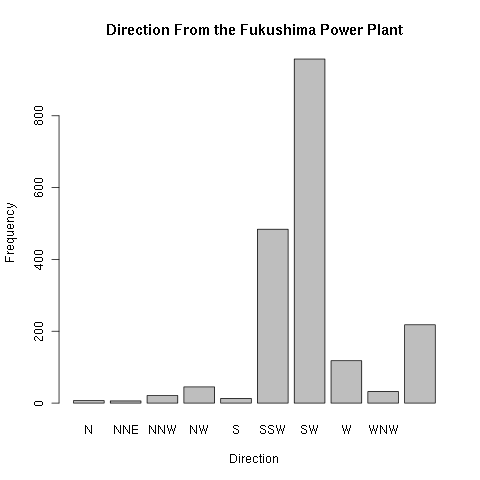
\includegraphics[width=8cm]{img/fukushimaDirectionBarPlot}
  \end{center}

\end{frame}

\begin{frame}
  \frametitle{Direction - Pareto Chart}

  \begin{center}
    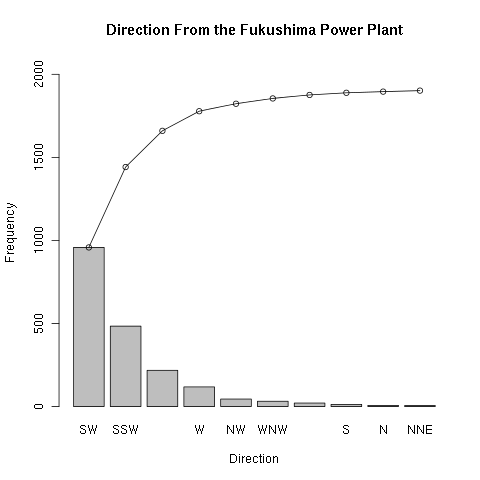
\includegraphics[width=8cm]{img/fukushimaParetoDirection}
  \end{center}

\end{frame}

\begin{frame}
  \frametitle{Radiation Data}

  \begin{center}
    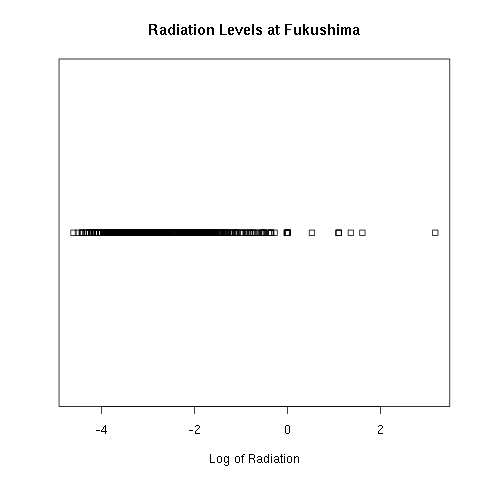
\includegraphics[width=8cm]{img/logFukushimaGamma}
  \end{center}  

\end{frame}

\begin{frame}
  \frametitle{Radiation Data}

  \begin{center}
    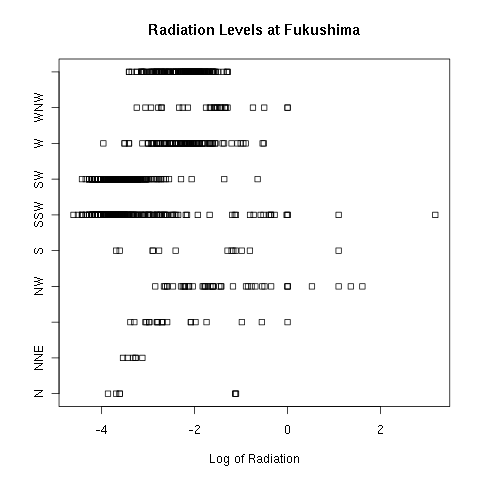
\includegraphics[width=8cm]{img/logFukushimaGammaByDirection}
  \end{center}  

\end{frame}


\begin{frame}{Why is the data spread out?}

  Problem: The data has a random component. Different measurements at
  different times give different radiation levels. 

  \vfill

  There is spread in the data and there are probabilities associated
  with how likely you are to get a certain range of measurements.

  \vfill
  
\end{frame}

\begin{frame}{Probability}

  What is probability?

  \begin{definition}[Probability]
    ``\textbf{Probability} is the measure of the likelihood of a random
    phenomena or chance behavior. Probability describes the long-term
    proportion with which a certain \textbf{outcome} will occur in
    situations with short-term uncertainty.'' (Page 223)
  \end{definition}

  
\end{frame}

\begin{frame}{Example}

  Everybody flip a coin once.

  \uncover<2->%
  {

    What did you get?

  }

  \uncover<3->%
  {

    Do it again!

  }

  \uncover<4->%
  {

    What did you get?

  }

  \uncover<5->%
  {

    Do it again!

  }

  \uncover<6->%
  {

    What did you get?

  }


  \uncover<7->%
  {

    (Four people) Flip a coin

  }

  \uncover<8->%
  {

    What did you get?

  }

  
\end{frame}

\begin{frame}{What the heck are we doing?}

  \begin{description}
  \item[Event:] Something that \textit{can} happen.
  \item[Outcome:] Something that did happen.
  \item[Experiment:] A structured activity that includes the
    measurement of the outcomes of the activity after predefined and
    intentional changes to some aspect of the events.
  \item[Observational Study:] A structured activity that includes the
    measurement of the outcomes of the activity without intentional
    changes to the events.
  \item[Expected Outcome:] The ``average'' of the possible outcomes.
  \item[Variation:] Some measure of the spread of possible outcomes.
  \end{description}
  
\end{frame}

\begin{frame}{Probability vs. Statistics}

  ``Probability'' is an idealized notion. If we repeat the experiment
  an infinite number of times we ask what \textit{will} happen.

  \vfill

  ``Statistics'' is the study of how to interpret data. We ask what
  ``did'' happen and what does it imply about the underlying
  probabilities?

  \vfill

  \uncover<2->%
  {

    Problem: We need to have a basic understanding of probability
    before we can do statistics.

  }
  
\end{frame}

% LocalWords:  Clarkson pausesection hideallsubsections Cuby Webworks Webwork
% LocalWords:  ResponseCard Fukushima hideothersubsections sectionstyle


% %%%%%%%%%%%%%%%%%%%%%%%%%%%%%%%%%%%%%%%%%%%%%%%%%%%%%%%%%%%%

\lecture{Introduction to Probability}{intro-to-probability}
\section{Introduction to Probability}

\title{Probability}
\subtitle{What are the chances?}

%\author{Kelly Black}
%\institute{Clarkson University}
\date{14 January 2013}

\begin{frame}
  \titlepage
\end{frame}

\begin{frame}
  \frametitle{Outline}
  \tableofcontents[hideothersubsections,sectionstyle=show/hide]
\end{frame}


\subsection{Clicker Quiz}


\iftoggle{clicker}{%

  \begin{frame}
    \frametitle{Clicker Quiz}

    If I flip a fair coin ten times how many tails will I get?

    \begin{tabular}{l@{\hspace{3em}}l@{\hspace{3em}}l@{\hspace{3em}}l}
      A: 4 & B: 5 & C: 6 & D: I do not know
    \end{tabular}


  \end{frame}

}




\subsection{Example}

%\begin{frame}
%  \frametitle{Clicker Exercise}
%
%  Flip a coin 3 times. How many tails did you get?
%
%  \begin{tabular}{l@{\hspace{3em}}l@{\hspace{3em}}l@{\hspace{3em}}l}
%  A: 0 & B: 1 & C: 2 & D: 3
%  \end{tabular}
%
%  \only<2->%
%  {
%    Question: What is the probability that we get the same result if
%    we do it again?
%  }
%
%\end{frame}

\begin{frame}{Recall}

  Recall from last time:

  \begin{definition}[Probability]
    ``\textbf{Probability} is the measure of the likelihood of a random
    phenomena or chance behavior. Probability describes the long-term
    proportion with which a certain \textbf{outcome} will occur in
    situations with short-term uncertainty.'' (Page 223)
  \end{definition}

  
\end{frame}


\begin{frame}{Also Recall}

  \begin{description}
  \item[Event:] Something that \textit{can} happen.
  \item[Outcome:] Something that did happen.
  \item[Experiment:] A structured activity that includes the
    measurement of the outcomes of the activity after predefined and
    intentional changes to some aspect of the events.
  \item[Observational Study:] A structured activity that includes the
    measurement of the outcomes of the activity without intentional
    changes to the events.
  \item[Expected Outcome:] The ``average'' of the possible outcomes.
  \item[Variation:] Some measure of the spread of possible outcomes.
  \end{description}
  
\end{frame}

\begin{frame}{Also Also Recall}

  ``Probability'' is an idealized notion. If we repeat the experiment
  an infinite number of times we ask what \textit{will} happen.

  \vfill

  ``Statistics'' is the study of how to interpret data. We ask what
  ``did'' happen and what does it imply about the underlying
  probabilities?

  \vfill

\end{frame}


\subsection{Events}

\begin{frame}
  \frametitle{Events}

  \begin{definition}
    An event is a possible outcome from an experiment.
  \end{definition}

\end{frame}


\begin{frame}
  \frametitle{Sample Space}

  \begin{definition}
    The sample space is the collection of all possible events.
  \end{definition}

\end{frame}


\begin{frame}
  \frametitle{Sample Space}

  There are two ways to visualize the sample space:
  \begin{itemize}
  \item Venn Diagram
  \item Tree Diagram
  \end{itemize}

\end{frame}

\subsection{Examples}

\begin{frame}{Example}

  We flip a coin two times. What are the events?

  \only<2->%
  {

    \begin{eqnarray*}
      p(\mathrm{first~T}) & = & ? \\
      p(TT) & = & ? \\
      p(TH) & = & ? \\
      p(\mathrm{second~H}) & = & ? \\
      p(\mathrm{one~T}) & = & ? \\
      p(\mathrm{two~H}) & = & ?
    \end{eqnarray*}

  }
  
\end{frame}

\begin{frame}{Clicker Quiz}
  A couple has a child. Two years later they have another child. What
  is the probability that they have one girl and one boy?

  \begin{tabular}{l@{\hspace{3em}}l@{\hspace{3em}}l@{\hspace{3em}}l}
    A: 0 & B: 1/4 & C: 1/2 & D: 1
  \end{tabular}


\end{frame}

\begin{frame}{Example}

  I roll a die twice. What is $p(\mathrm{sum}=5)$?
  
\end{frame}


\subsection{Properties of Probabilities}

\begin{frame}{Properties of Probabilities}

  Suppose that A is an event in the sample space, then
  \begin{eqnarray*}
    \begin{array}{rcccl}
      0 & \leq & P(A) & \leq & 1
    \end{array}
  \end{eqnarray*}
  
\end{frame}


% LocalWords:  Clarkson pausesection hideallsubsections


\lecture{Probability Rules}{probability-rules}
\section{Probability Rules}

\title{Probability Rules}
\subtitle{Calculating Probabilities}

%\author{Kelly Black}
%\institute{Clarkson University}
\date{16 January 2013}

\begin{frame}
  \titlepage
\end{frame}

\begin{frame}
  \frametitle{Outline}
  \tableofcontents[pausesection,hideothersubsections,sectionstyle=show/hide]
\end{frame}



\iftoggle{clicker}{%
  \subsection{Clicker Quiz}


  \begin{frame}
    \frametitle{Clicker Quiz}

    I have a bag with eight marbles. Five marbles are red and three are
    blue. I pull one marble out at random. What is the probability that
    it is red?

    \begin{tabular}{l@{\hspace{3em}}l@{\hspace{3em}}l@{\hspace{3em}}l}
      A: 3/8 & B: 5/8 & C: 1
    \end{tabular}


  \end{frame}
}


\subsection{Examples}

\begin{frame}{Example}

  I roll a six-sided die. What is the probability that I roll a one?

  \only<2->%
  {
    I roll a six-sided die. What is the probability that I roll a one
    \textbf{or} a two?
  }

  \only<3->%
  {
    I roll a six-sided die. What is the probability that I roll an odd
    number?
  }

  \only<4->%
  {
    I roll a six-sided die. What is the probability that I roll an odd
    number \textbf{or} a number less than 3?
  }

  
\end{frame}


\begin{frame}{Something does not add up}

  \begin{eqnarray*}
    p(\mathrm{odd}) & = & \frac{3}{6}, \\
    p(\mathrm{number}<3) & = & \frac{2}{6}, \\
  \end{eqnarray*}

  \only<2->%
  {

    \begin{eqnarray*}
      p(\mathrm{odd}) + p(\mathrm{number}<3) & = & \frac{5}{6}, \\
      p(\mathrm{odd~or~\mathrm{number}<3}) & = & \frac{4}{6}.
    \end{eqnarray*}
    they are not the same!

  }

  
\end{frame}


\begin{frame}{Example}

  I roll a six-sided die. What is the probability that I roll an odd
  \textbf{and} a number less than 3?
  
\end{frame}

\begin{frame}{In General}

  What is $p(A~or~B)$?

  \only<1>{\includegraphics[width=5cm]{img/vennDiagram}}
  \only<2->{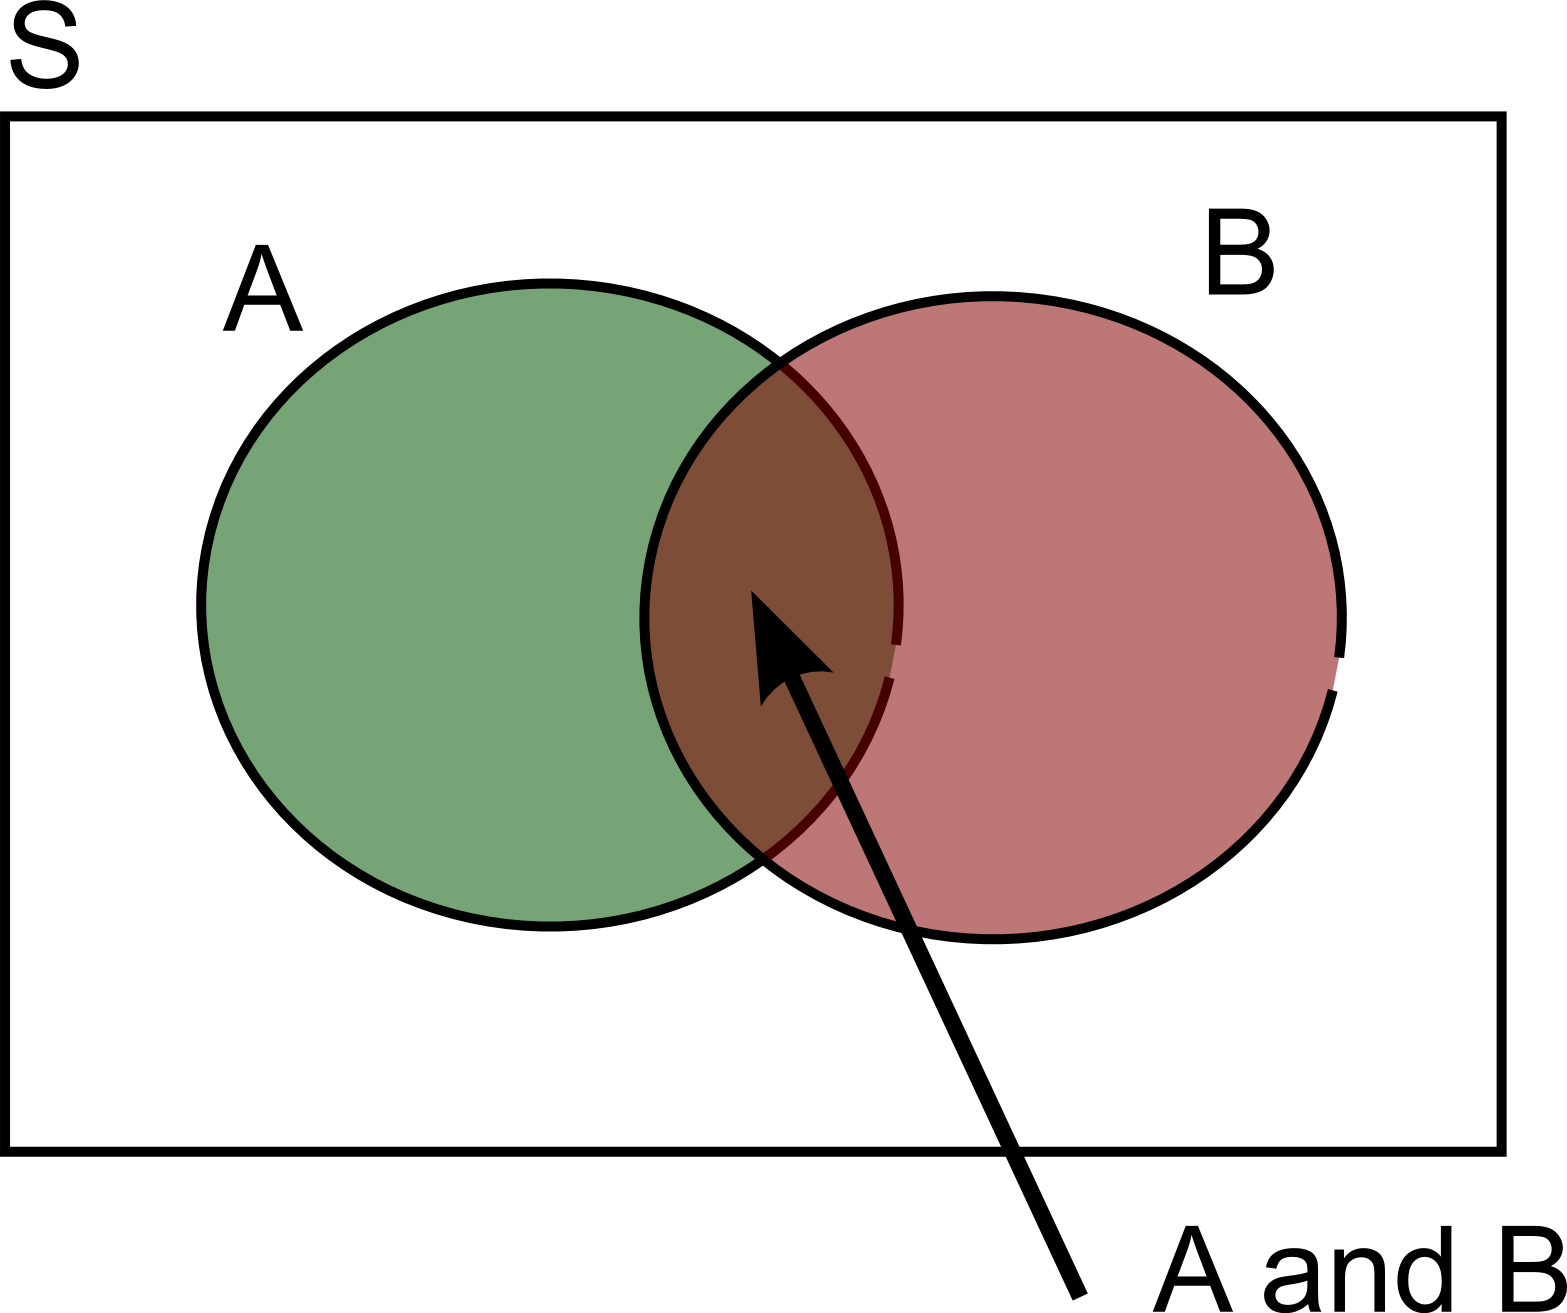
\includegraphics[width=5cm]{img/vennDiagramAnnotated}}
  \only<3->%
  {

    \begin{eqnarray*}
      p(\mathrm{A~or~B}) & = & p(A) + p(B) - p(\mathrm{A~and~B})
    \end{eqnarray*}
    Be careful about the discussion in the book about ``disjoint sets.''

  }
  
\end{frame}

\subsection{Compliment}

\begin{frame}{Compliment}

  The compliment of a set is everything not in the set.
  \only<1>{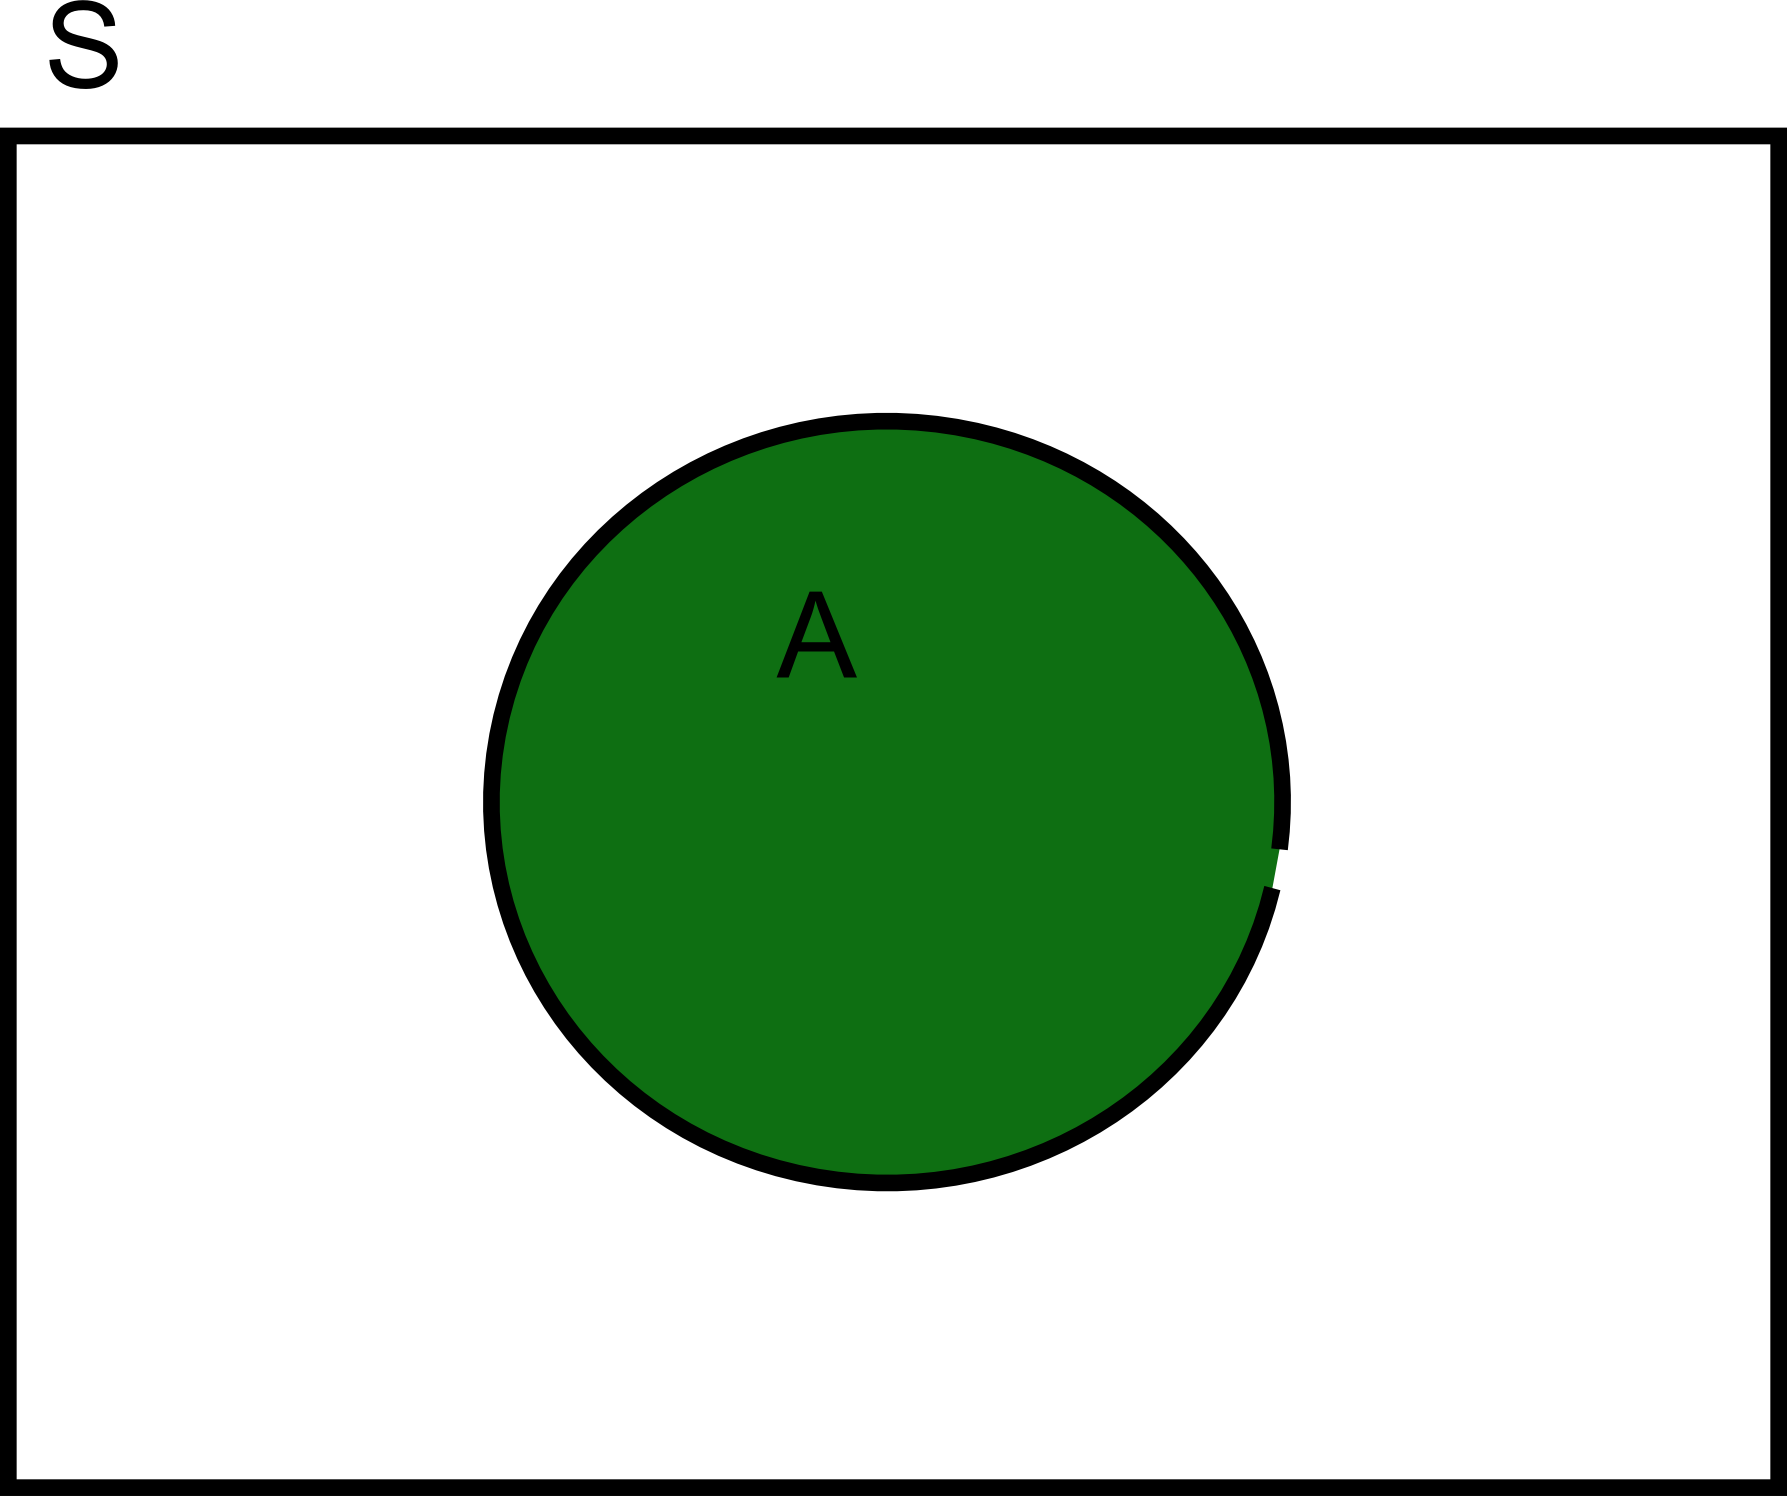
\includegraphics[width=5cm]{img/complimentVennOne}}
  \only<2>{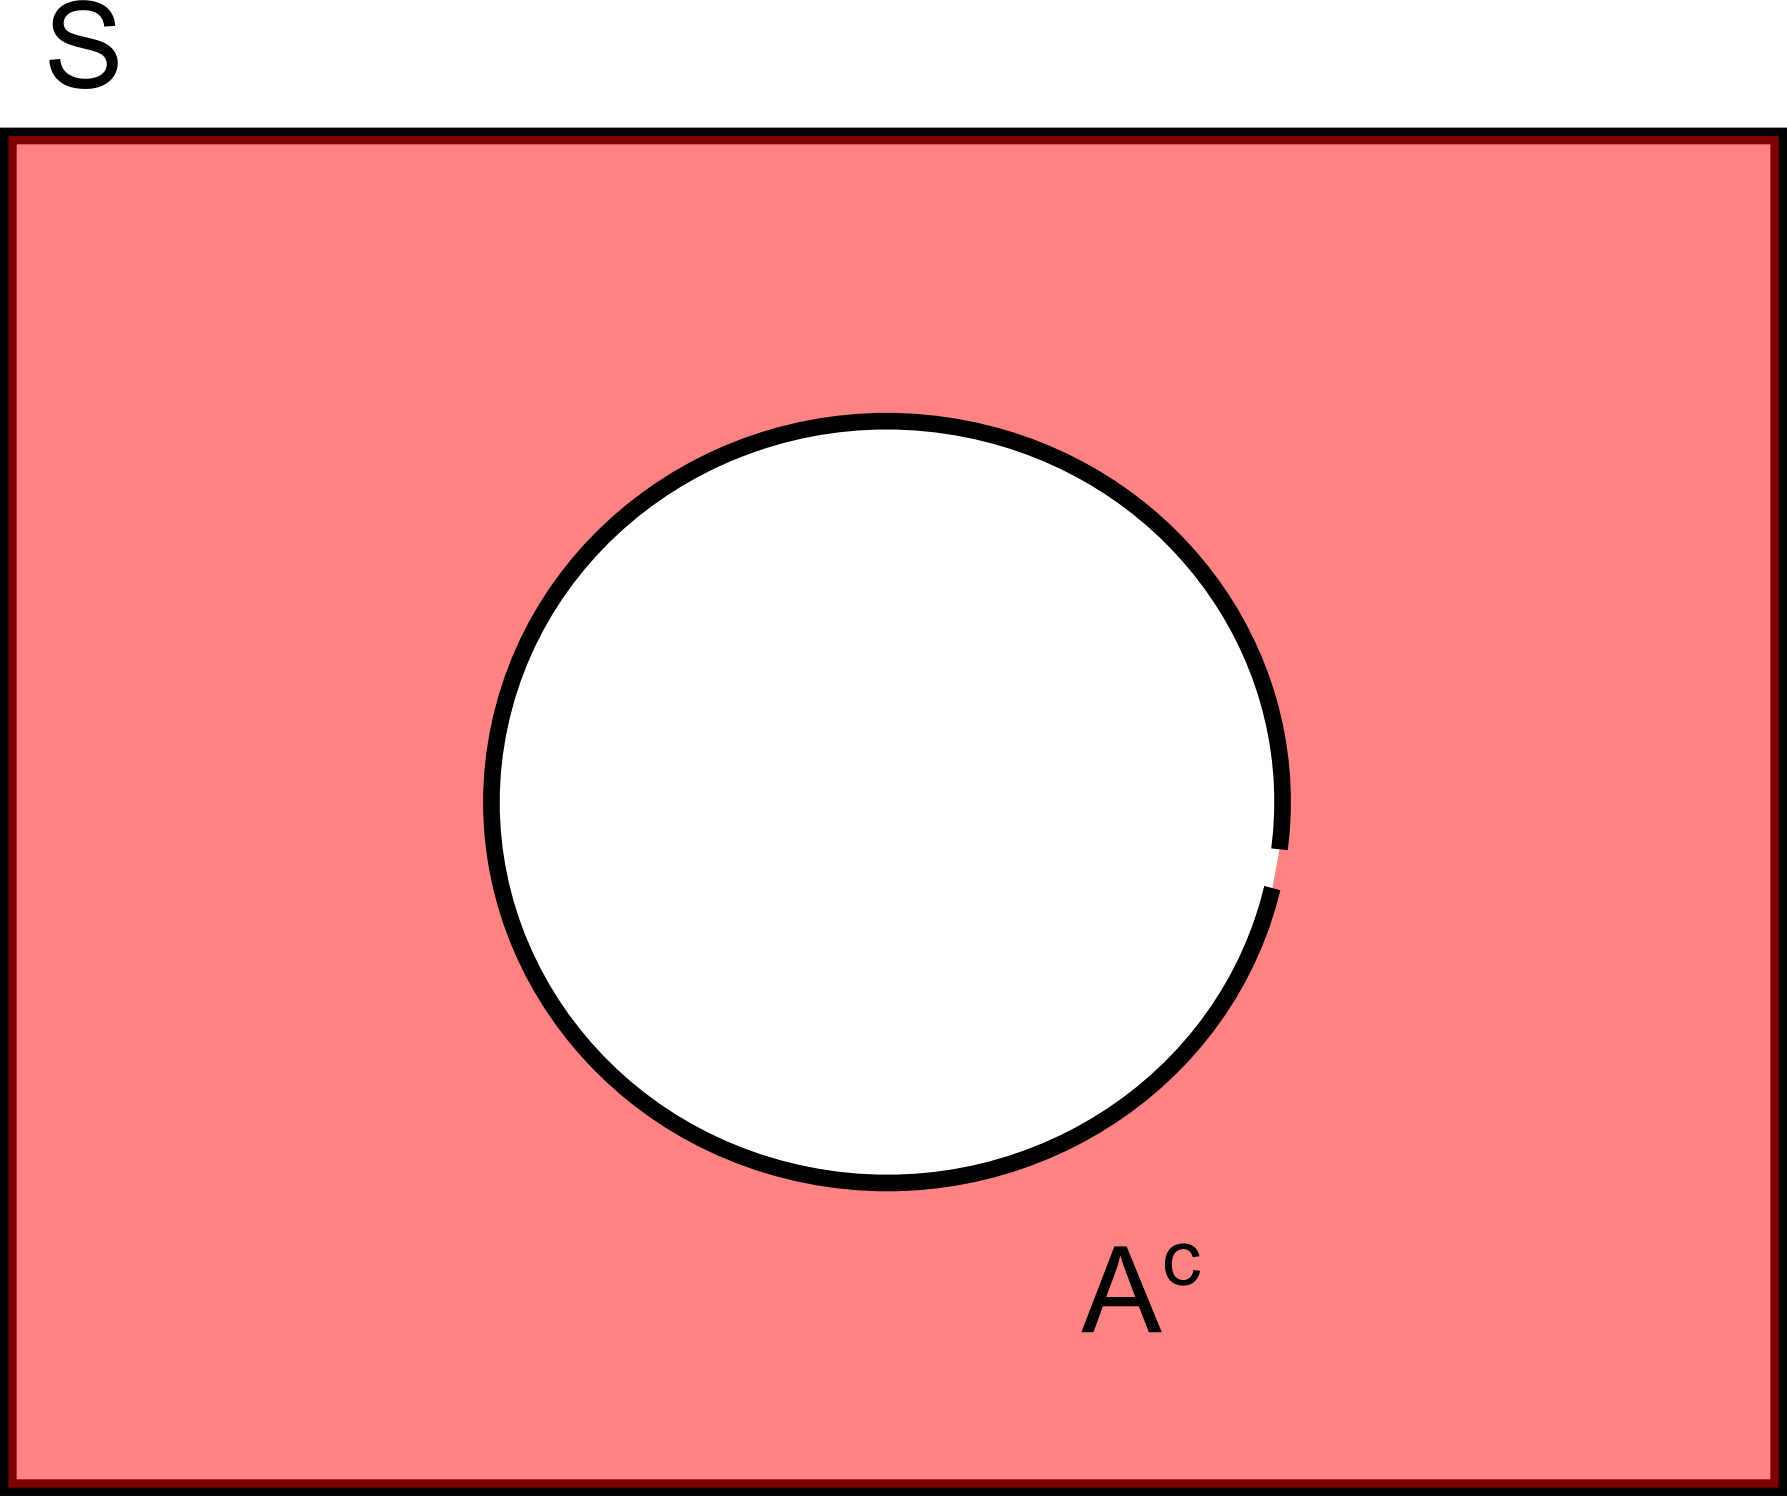
\includegraphics[width=5cm]{img/complimentVennTwo}}

  Notation:
  \begin{eqnarray*}
    A^c & = & \mathrm{Compliment~of~A}.
  \end{eqnarray*}

  
\end{frame}

\begin{frame}{Compliment}

  \begin{definition}
    Suppose $A$ is an event. Then all of the events not in A are denoted
    by $A^C$. 

    Other notations:
    \begin{eqnarray*}
      \bar{A},~A'.
    \end{eqnarray*}
  \end{definition}


\end{frame}




\begin{frame}{Probabilities of Compliments}
  
  \begin{eqnarray*}
    1 & = & p(A) + p(\bar{A}), \\
    p(A) & = & 1 - p(\bar{A}).
  \end{eqnarray*}

\end{frame}


\begin{frame}{Example}

  Number of drivers killed in fatal automobile crashes in 2005: \\
  \begin{tabular}{llll}
    Age & Male & Female & Total \\
    $<$16 & 227 & 77 & 304 \\
    16-20 & 5180 & 2113 & 7293 \\
    21-34 & 13611 & 4311 & 17922 \\
    35-54 & 15108 & 5027 & 20135 \\
    55-74 & 6801 & 2452 & 9253 \\
    $>$74   & 2022 & 980 & 3002 \\
    Total & 42949 & 14960 & 57909 
  \end{tabular} \\

  \vfill

  \textit{Traffic Safety Facts 2005, Federal Highway Administration,
    2005}

  \vfill

  I pick one person at random. What is the probability that the person
  is male and has an age between 21 and 34?

  
  
\end{frame}


\begin{frame}{Example}

  Number of drivers killed in fatal automobile crashes in 2005: \\
  \begin{tabular}{llll}
    Age & Male & Female & Total \\
    $<$16 & 227 & 77 & 304 \\
    16-20 & 5180 & 2113 & 7293 \\
    21-34 & 13611 & 4311 & 17922 \\
    35-54 & 15108 & 5027 & 20135 \\
    55-74 & 6801 & 2452 & 9253 \\
    $>$74   & 2022 & 980 & 3002 \\
    Total & 42949 & 14960 & 57909 
  \end{tabular} \\

  \vfill

  \textit{Traffic Safety Facts 2005, Fedoral Highway Administration,
    2005}

  \vfill

  I pick one person at random. What is the probability that the person
  is male or has an age between 21 and 34?

  
  
\end{frame}


\begin{frame}{Example}

  Number of drivers killed in fatal automobile crashes in 2005: \\
  \begin{tabular}{llll}
    Age & Male & Female & Total \\
    $<$16 & 227 & 77 & 304 \\
    16-20 & 5180 & 2113 & 7293 \\
    21-34 & 13611 & 4311 & 17922 \\
    35-54 & 15108 & 5027 & 20135 \\
    55-74 & 6801 & 2452 & 9253 \\
    $>$74   & 2022 & 980 & 3002 \\
    Total & 42949 & 14960 & 57909 
  \end{tabular} \\

  \vfill

  \textit{Traffic Safety Facts 2005, Federal Highway Administration,
    2005}

  \vfill

  I pick one person at random. What is the probability that the person's
  age is less that 74?

  
  
\end{frame}


\iftoggle{clicker}{%
  \begin{frame}{Clicker Quiz}

    Number of drivers killed in fatal automobile crashes in 2005: \\
    \begin{tabular}{llll}
      Age & Male & Female & Total \\
      $<$16 & 227 & 77 & 304 \\
      16-20 & 5180 & 2113 & 7293 \\
      21-34 & 13611 & 4311 & 17922 \\
      35-54 & 15108 & 5027 & 20135 \\
      55-74 & 6801 & 2452 & 9253 \\
      $>$74   & 2022 & 980 & 3002 \\
      Total & 42949 & 14960 & 57909 
    \end{tabular} \\

    \vfill

    \textit{Traffic Safety Facts 2005, Federal Highway Administration,
      2005}

    \vfill

    I pick one person at random. What is the probability that the person
    is female or age is between 16 and 20?

    \begin{tabular}{l@{\hspace{3em}}l@{\hspace{3em}}l@{\hspace{3em}}l}
      A: $\frac{2113}{57,909}$ & B:$\frac{14960}{57,909}$  \\ C:
      $\frac{2113}{57,909}+\frac{77}{57,909}$ &
      D: $\frac{14960}{57,909}+\frac{7293}{57,909}-\frac{2113}{57,909}$
    \end{tabular}
  
  
\end{frame}
}



\subsection{Conditional Probability}

\begin{frame}
  \frametitle{Example }

  1000 voters are polled in the 2008 election. We get the following
  information: \\
  \only<1>
  {
    \begin{tabular}{l|l|l|l}
      Education & Obama & McCain & Others  \\ \hline
      No H.S. Diploma & 19 & 20 & 1   \\
      H.S. Diploma only & 114 & 103 & 3 
    \end{tabular}
  }
  \only<2->
  {
    \begin{tabular}{l|l|l|l|l}
      Education & Obama & McCain & Others & Total \\ \hline
      No H.S. Diploma & 19 & 20 & 1 & 40 \\
      H.S. Diploma only & 114 & 103 & 3 & 220 \\ \hline
      Total & 133 & 123 & 4 & 260
    \end{tabular}
  }



\end{frame}


%\begin{frame}{Clicker Quiz}
%
%
%  A bowl has candy. Eight of the candies are chocolate, and of the
%  chocolates three have red wrappers while the rest have silver
%  wrappers. Twelve of the candies are hard candy, and of the hard
%  candies four have red wrappers while the rest have silver
%  wrappers. I pull out one candy at random, and it is a
%  chocolate. What is the probability that it has a red wrapper?
%
%  \begin{tabular}{l@{\hspace{3em}}l@{\hspace{3em}}l@{\hspace{3em}}l}
%    A: 4/12 & B: 3/8 & C: 5/8 & D: 8/12
%  \end{tabular}
%
%  
%\end{frame}




% LocalWords:  Clarkson pausesection hideallsubsections Obama


\lecture{Probability Rules}{probability-rules}
\section{Probability Rules}

\title{Probability Rules}
\subtitle{Putting it All Together}

%\author{Kelly Black}
%\institute{Clarkson University}
\date{16 January 2015}

\begin{frame}
  \titlepage
\end{frame}

\begin{frame}
  \frametitle{Outline}
  \tableofcontents[hideothersubsections,sectionstyle=show/hide]
\end{frame}


\subsection{Clicker Quiz}


\iftoggle{clicker}{%
  \begin{frame}
    \frametitle{Clicker Quiz}

    I have a bag with ten blue marbles and four red marbles. I remove
    one marble and put it to the side. The marble was a blue
    marble. What is the probability that I pull out a blue marble the
    next time I draw a marble?

    \vspace{2em}

    \begin{tabular}{l@{\hspace{3em}}l@{\hspace{3em}}l@{\hspace{3em}}l}
      A: $\frac{10}{14}$ & B: $\frac{9}{13}$ & C: $\frac{4}{14}$ & D: $\frac{4}{13}$
    \end{tabular}

    \vfill

  \end{frame}
}

\begin{frame}
  \frametitle{Verbiage Issues}

  I have a bag with ten blue marbles and four red marbles. I remove
  one marble \textbf{\color{red}{without replacement}}. The marble was
  a blue marble. What is the probability that I pull out a blue marble
  the next time I draw a marble?

    \vfill

\end{frame}

\begin{frame}{I Know Things}

  Problem: Sometimes I know something about what
  occured. \textit{\textbf{Given}} that information how do I incorporate it
  into the probability that some event occured?

  \vfill
  \includegraphics[width=5cm]{img/vennDiagram}
  \vfill
  
\end{frame}

\begin{frame}
  \frametitle{Example From Last Time}

  1000 voters are polled in the 2008 election. We get the following
  information: \\
  \only<1>
  {
    \begin{tabular}{l|l|l|l}
      Education & Obama & McCain & Others  \\ \hline
      No H.S. Diploma & 19 & 20 & 1   \\
      H.S. Diploma only & 114 & 103 & 3 
    \end{tabular}
  }
  \only<2->
  {
    \begin{tabular}{l|l|l|l|l}
      Education & Obama & McCain & Others & \color{red}{Total} \\ \hline
      No H.S. Diploma & 19 & 20 & 1 & \color{red}{40} \\
      H.S. Diploma only & 114 & 103 & 3 & \color{red}{220} \\ \hline
      \color{red}{Total} & \color{red}{133} & \color{red}{123} & \color{red}{4} & \color{blue}{260}
    \end{tabular}
  }

  \vfill

  \visible<3->{%
    \textcolor<4>{gray}{
      I choose one of these people at random, and I know that the person
      voted for President Obama. What is the probability that the person
      has no high school diploma?
    }
  }

  \uncover<4->{%
    I choose one of these people at random, and I know that the person
    has no high school diploma. What is the probability that the
    person voted for President Obama?
  }


\end{frame}



\begin{frame}{Conditional Probability}

  I know that B occured. Given that information, what is the
  probability that A occured?

  \begin{definition}{Conditional Probability}

    The probability that A occurs given that I know that B occured is
    denoted by
    \begin{eqnarray*}
      p(A|B).
    \end{eqnarray*}
    
  \end{definition}
  
\end{frame}




\begin{frame}{Conditional Probability}

  \includegraphics[width=5cm]{img/vennDiagram}

  I know that B occured. Given that information, what is the
  probability that A occured?

  
\end{frame}

\begin{frame}
  \frametitle{Conditional Probability}

  \begin{definition}
    The probability that A occurs given that I know that B occured is
    defined to be 
    \begin{eqnarray*}
      p(A|B) & = & \frac{p(A \mathrm{~and~} B)}{p(B)}, \\
      \mathrm{or~} 
      p(B) p(A|B)  &  =  & p(A \mathrm{~and~} B).
    \end{eqnarray*}
  \end{definition}

\end{frame}


\begin{frame}{Example 2}

  I have a bag with eight marbles. Five marbles are red and three are
  blue. I pick two, one after the other \textcolor<2->{red}{without
    replacement}. \textcolor<2->{blue}{What is the probability that I pull
    out a red and then a blue marble?}

  \vfill

  \visible<3->%
  {
    \textcolor<4->{gray}{
      What is the probability that I get exactly one red marble?
    }
  }
  
  \vfill

  \visible<4->%
  {
    \textcolor<5->{gray}{
      What is the probability that I get two red marbles?
    }
  }
  
  \vfill

  \visible<5->%
  {
      What is the probability that I get no red marbles?
  }
  
  \vfill


\end{frame}


\subsection{Probability Rules}

\begin{frame}{Probability Rules}

  \begin{definition}
    The multiplication rule:
    \begin{eqnarray*}
      p(A)\cdot p(B|A) & = & p(A \mathrm{~and~} B), \\
      p(B)\cdot p(A|B) & = & p(A \mathrm{~and~} B).
    \end{eqnarray*}

    The addition rule:
    \begin{eqnarray*}
      p(A \mathrm{~or~} B) & = & p(A) + p(B) - p(A \mathrm{~and~} B).
    \end{eqnarray*}

    The compliment rule:
    \begin{eqnarray*}
      p(A^c) & = & 1 - p(A).
    \end{eqnarray*}

  \end{definition}

  \vfill
  
\end{frame}


\subsection{Examples}

\begin{frame}
  \frametitle{Example 1}

  \vfill

  A ball is hidden under one of three cups. You pay \$5.00 to find the
  ball. You get \$10.00 if you find it on your first guess. You get
  \$2.00 if you get it on your second guess. Otherwise you get
  nothing.

  \vfill

  What is the probability of getting some money back?

  \vfill

\end{frame}


\begin{frame}
  \frametitle{Clicker Quiz}
  
  \vfill

  A store sells skates. Thirty percent of the skates are used. Five
  percent of the new skates are defective. Twenty percent of the used
  skates are defective. You pick one set of skates out at random. What
  is the probability that the set is defective?

  \vfill

  \begin{tabular}{l@{\hspace{3em}}l@{\hspace{3em}}l@{\hspace{3em}}l}
    A: 0.050  & B: .095  & C: .110 & D: .250
  \end{tabular}

  \vfill

\end{frame}


\begin{frame}{Example}

  \vfill

  A test can detect the presence of an abnormal gene that causes cystic
  fibrosis (CF). It is estimated that about 5\% of all people have the
  abnormal gene. The test is correct 90\% of the time for people who
  have the abnormal gene. About 2\% of the time it is positive for
  people who do not have the abnormal gene.

  \vfill

  If someone tests positive for the abnormal gene what is the
  probability that they have the abnormal gene?

  \vfill
  
\end{frame}

\begin{frame}
  \frametitle{Example}

  I have a bag with ten blue marbles and four red marbles. I remove
  two marbles \textcolor<2->{red}{without
    replacement}. \textcolor<2->{blue}{What is the probability that I
    pull out at least one blue marble?}


  \vfill

\end{frame}



% LocalWords:  Clarkson pausesection hideallsubsections hideothersubsections
% LocalWords:  sectionstyle Obama

%
\lecture{Independence And Mutual Exclusion}{indepence-and-mutual-exclusion}
\section{Independence And Mutual Exclusion}

\title{Independence And Mutual Exclusion}
\subtitle{Stuff We Already Did}

%\author{Kelly Black}
%\institute{Clarkson University}
\date{3 Feb 2012}

\begin{frame}
  \titlepage
\end{frame}

\begin{frame}
  \frametitle{Outline}
  \tableofcontents[pausesection,hideothersubsections,sectionstyle=show/hide]
\end{frame}


\subsection{Clicker Quiz}


\begin{frame}
  \frametitle{Clicker Quiz}

  If $p(A)=0.3$, $p(B)=0.4$, and $p(A\mathrm{~or~}B)=.37$ what is
  $p(A\mathrm{~and~}B)$?

  \vfill

  \begin{tabular}{l@{\hspace{3em}}l@{\hspace{3em}}l}
    A: .11 & B: 12 & C: .33
  \end{tabular}

  \vfill
  \vfill
  \vfill

\end{frame}




\subsection{Example}

\begin{frame}
  \frametitle{Example 1}

  I flip a coin two times. What is the probability that I get a tails
  on the second flip?

  \vfill


\end{frame}


\subsection{Mutually Exclusive Events}

\begin{frame}
  \frametitle{Mutual Exclusion}

  \begin{definition}
    Two sets are \textit{mutually exclusive} if they have nothing in
    common.
  \end{definition}

\end{frame}


\begin{frame}{Example 2}
  
  I have a bag with six red marbles and two blue marbles. I draw two
  without replacement. What is the probability that the second marble
  is red?

  \vfill

\end{frame}

\subsection{Independent Events}

\begin{frame}
  \frametitle{Independence}

  \begin{definition}
    Two events are independent if 
    \begin{eqnarray*}
      p(A|B) & = & p(A).
    \end{eqnarray*}

    This is equivalent to requiring that
    \begin{eqnarray*}
      p(B|A) & = & p(B).
    \end{eqnarray*}

  \end{definition}

\end{frame}



\begin{frame}{Example 3}

  Suppose that $p(A)=0.6$, $p(B)=0.3$, and $p(A\mathrm{~and~}B)=.2$
  Are they independent?

  \vfill

  
\end{frame}



\begin{frame}{Example 4}

  Suppose that $p(A)=0.6$, $p(B)=0.3$, and $p(A\mathrm{~and~}B)=.18$
  Are they independent?

  \vfill

  
\end{frame}


\begin{frame}{Example 5}
  An industrial process is established to produce items. About five
  percent of the items are defective under this process. Each item is
  inspected, and fifteen percent of the defective items are not caught
  in the inspection. About three percent of the good items are
  classified as defective.

  \begin{itemize}
  \item What percentage of the items that are sold are defective?
  \item I pick a part at random. That part is classified as
    defective. What is the probability that it is actually defective?
  \end{itemize}

  \vfill

\end{frame}


\begin{frame}{Example 6}

  A brokerage firm has a system that can execute a sell request in
  within 0.08 seconds about 85\% of the time. Of the requests that
  occur within 0.08 seconds about 75\% meet the projected cost
  level. Of the requests that do not occur within 0.08 seconds about
  65\% meet the projected cost level.

  What is the proportion of requests that will meet the projected cost
  levels?

  \vfill
  
\end{frame}




% LocalWords:  Clarkson pausesection hideallsubsections

% %%%%%%%%%%%%%%%%%%%%%%%%%%%%%%%%%%%%%%%%%%%%%%%%%%%%%%%%%%%%

\lecture{Counting}{counting}
\section{Counting}

\title{Counting}
\subtitle{Stuff We Thought We Knew}

%\author{Kelly Black}
%\institute{Clarkson University}
\date{21 January 2013}

\begin{frame}
  \titlepage
\end{frame}

\begin{frame}
  \frametitle{Outline}
  \tableofcontents[pausesection,hideothersubsections,sectionstyle=show/hide]
\end{frame}


\iftoggle{clicker}{%
  \subsection{Clicker Quiz}


  \begin{frame}
    \frametitle{Clicker Quiz}

    If $p(A)=0.8$, $p(B|A)=0.4$ what is $p(A\mathrm{~and~}B)$?

    \vfill

    \begin{tabular}{l@{\hspace{3em}}l@{\hspace{3em}}l}
      A: .32 & B: 0.50 & C: 2.0
    \end{tabular}

    \vfill
    \vfill
    \vfill

  \end{frame}

}

\subsection{Multiplication Rule}

\begin{frame}
  \frametitle{How Many Ways?}
  Suppose that I flip a fair coin three times. How many possible
  outcomes are there?

  \vfill

\end{frame}

\begin{frame}{Example}

  I have three pairs of pants and two shirts. How many different
  outfits do I have?

  \vfill
  
\end{frame}

\begin{frame}
  \frametitle{Multiplication Rule}

  \begin{definition}[The Multiplication Rule]
    If I have choices where I have
    \begin{itemize}
    \item $p_1$ choices for the first item
    \item $p_2$ choices for the second item
    \item $p_3$ choices for the third item \\
      $\vdots$
    \item $p_k$ choices for the $k$\textsuperscript{th} item \\
    \end{itemize}

    The total number of possible selections is 
    \begin{eqnarray*}
      p_1 \cdot p_2 \cdot p_3 \cdots ~ \cdot p_k.
    \end{eqnarray*}

  \end{definition}

\end{frame}

\subsection{Permutations}

\begin{frame}
  \frametitle{Example}
  A committee has eight people. There is a chair and a secretary for
  the committee. How many ways are there to choose a chair and a
  secretary?

  \vfill

  \textit{ order matters!}

\end{frame}

\begin{frame}
  \frametitle{Example}
  Twelve people are in a race. The first three people get an
  award. How many different ways can we hand out the awards?

  \vfill

  \textit{ order matters!}
\end{frame}


\begin{frame}
  \frametitle{Permutations}
  \begin{definition}[Permutations]
    The number of permutations is the number of ways to arrange $n$
    objects when $r$ is chosen. \textit{(The order matters.)}
  \end{definition}

  \only<2->%
  {
    \begin{definition}[Notation]
      The number of permutations for $n$ objects when you choose $r$
      is 
      \begin{eqnarray*}
        \prescript{~}{n}{P}_r.
      \end{eqnarray*}
    \end{definition}
  }

\end{frame}

\begin{frame}
  \frametitle{Previous Examples}

  \begin{eqnarray*}
    \prescript{~}{8}{P}_2 & = & 8\cdot 7, \\
    \prescript{~}{12}{P}_3 & = & 12\cdot 11 \cdot 10. \\
  \end{eqnarray*}


  \only<2->%
  {

    \begin{definition}[General Formula for Permutations]

      In general
      \begin{eqnarray*}
        \prescript{~}{n}{P}_r & = & n(n-1)(n-2)\cdots(n-r+1).
      \end{eqnarray*}

      
    \end{definition}

  }
  
\end{frame}

\begin{frame}
  \frametitle{Notation}

  \begin{definition}[Factorials]

    If $n$ is an integer then
    \begin{eqnarray}
      n! & = & n(n-1)(n-2)\cdot 3 \cdot 2 \cdot 1.
    \end{eqnarray}
    
  \end{definition}

  Examples:
  \begin{eqnarray}
    4! & = & 4 \cdot 3  \cdot 2 \cdot 1, \\
    5! & = & 5 \cdot 4 \cdot 3  \cdot 2 \cdot 1.
  \end{eqnarray}
  
\end{frame}



\begin{frame}
  \frametitle{By the Way}

      \begin{eqnarray*}
        \prescript{~}{n}{P}_r & = & n(n-1)(n-2)\cdots(n-r+1), \\
        & = & \frac{n!}{(n-r)!}.
      \end{eqnarray*}

  
\end{frame}

\iftoggle{clicker}{%


  \begin{frame}
    \frametitle{Clicker Quiz}

    There are eight distinct marbles in a bag. I pull three out one
    after the other and place them side by side from left to
    right. How many different ways can this be done?

    \vfill

    \begin{tabular}{l@{\hspace{3em}}l@{\hspace{3em}}l@{\hspace{3em}}l}
      A: $8!$ & B: $\frac{8!}{3!}$  & C: $\frac{8!}{5!}$ & C: $3!$
    \end{tabular}

    \vfill
    \vfill
    \vfill

  \end{frame}

}



\subsection{Combinations}

\begin{frame}
  \frametitle{Example}

  What if I have three people on a team but only two can play at a
  time? How many groups can play?

  \vfill

  \only<2->%
  {

    Notation:
    \begin{eqnarray*}
      \prescript{~}{3}C_2 & = & 3, \\
      3 \choose 2  & = & 3.
    \end{eqnarray*}

  }
  
\end{frame}


\begin{frame}
  \frametitle{Combinations}

  In general we have 
  \begin{eqnarray*}
    \underbrace{
      \rule{.3cm}{.2mm} \hspace{.05cm} 
      \rule{.3cm}{.2mm} \hspace{.05cm} 
      \rule{.3cm}{.2mm} \hspace{.05cm} 
      \rule{.3cm}{.2mm} \hspace{.05cm} 
      \rule{.3cm}{.2mm} \hspace{.05cm} \ldots
      \rule{.3cm}{.2mm} \hspace{.05cm} 
      \rule{.3cm}{.2mm} \hspace{.05cm}}_{\mathrm{n~possible~items}}
    & \rightarrow & 
    \underbrace{
      \rule{.3cm}{.2mm} \hspace{.05cm} 
      \rule{.3cm}{.2mm} \hspace{.05cm} 
      \rule{.3cm}{.2mm} \hspace{.05cm} \ldots
      \rule{.3cm}{.2mm} \hspace{.05cm} 
      \rule{.3cm}{.2mm} \hspace{.05cm}}_{\mathrm{k~slots}}
  \end{eqnarray*}

  \only<2->%
  {

    There are $\prescript{~}{n}{P}_r$ permutations. Each permutation
    can be expressed in $k!$ different ways,
    \begin{eqnarray*}
      \prescript{~}{n}{P}_r & = & k! \prescript{~}{n}{C}_r, \\
      \prescript{~}{n}{C}_r & = & \frac{\prescript{~}{n}{P}_r}{k!}, \\
      \prescript{~}{n}{C}_r & = & \frac{n!}{(n-k)!k!}.
    \end{eqnarray*}
  }
  
\end{frame}

\begin{frame}
  \frametitle{Example}
  Thirty people are on a committee. The executive committee is made up
  of four people. How many ways are there to form the executive
  committee?
  
\end{frame}

\iftoggle{clicker}{%


  \begin{frame}
    \frametitle{Clicker Quiz}

    There are eight distinct marbles in a bag. I pull three out one
    after the other and give them to a friend. How many different
    combinations can I give away?

    \vfill

    \begin{tabular}{l@{\hspace{3em}}l@{\hspace{3em}}l@{\hspace{3em}}l}
      A: $\frac{8!}{3!}$ & B: $\frac{8!}{5!3!}$  & C: $\frac{5!}{3!}$ & C: $3!$
    \end{tabular}

    \vfill
    \vfill
    \vfill

  \end{frame}

}


\subsection{Generalized Permutations}

\begin{frame}
  \frametitle{Generalized Permutations}

  I have
  \begin{itemize}
  \item A set of $n_1$ identical objects
  \item Another set of $n_2$ identical objects 
  \item Another set of $n_3$ identical objects \\
    \vdots
  \item Another set of $n_k$ identical objects, \\
  \item $n=n_1+n_2+n_3+\cdots+n_k$.
  \end{itemize}

  The number of ways to arrange these objects is 
  \begin{eqnarray*}
    \frac{n!}{n_1! n_2! n_3! \cdots n_k!}.
  \end{eqnarray*}
  
\end{frame}

\begin{frame}
  \frametitle{Example}

  I have five blue flags and eight red flags. How many ways can I
  arrange them on a vertical flag pole?

  
  
\end{frame}

%%% Local Variables: 
%%% mode: latex
%%% TeX-master: "IntroStats"
%%% End: 

% LocalWords:  pausesection hideothersubsections sectionstyle


\lecture{Random Variables}{random-variables}
\section{Random Variables}

\title{Random Variables}
\subtitle{Quantifying Outcomes}

%\author{Kelly Black}
%\institute{Clarkson University}
\date{8 February 2012}

\begin{frame}
  \titlepage
\end{frame}

\begin{frame}
  \frametitle{Outline}
  \tableofcontents[pausesection,hideothersubsections,sectionstyle=show/hide]
\end{frame}


\subsection{Clicker Quiz}


\begin{frame}
  \frametitle{Clicker Quiz}

  I flip a coin three times. What is the probability that I get two tails?

  \vfill

  \begin{tabular}{l@{\hspace{3em}}l@{\hspace{3em}}l}
    A: 1/8 & B: 3/8 & C: 1/2
  \end{tabular}

  \vfill
  \vfill
  \vfill

\end{frame}


\subsection{Random Variables}

\begin{frame}
  \frametitle{Random Variables}

  \begin{definition}
    A \textbf{random variable} is a variable whose outcome is a number
    and has a random component.
  \end{definition}

  \uncover<2->
  {
    \begin{definition}
      A \textbf{discrete random variable} is a random variable whose
      outcome is one of a countable number of outcomes.
    \end{definition}
  }

  \uncover<3->
  {
    \begin{definition}
      A \textbf{continuous random variable} is a random variable whose
      outcome come from a range of values.
    \end{definition}
  }

  \uncover<4->
  {
    \begin{definition}
      A \textbf{probability distribution} is a list of probabilities of
      \textit{all possible outcomes} of a random variable.
    \end{definition}
  }

\end{frame}



\begin{frame}{Discrete Random Variables}

  \begin{columns}
    \column{.40\textwidth}

    \begin{eqnarray*}
      \begin{array}{l|l}
        \mathrm{X} & p \\ \hline
        x_1 & p_1 \\
        x_2 & p_2 \\
        x_3 & p_3 \\
        \vdots & \vdots \\
        x_n & p_n
      \end{array}
    \end{eqnarray*}

    \column{.60\textwidth}
    Properties:
    \begin{eqnarray*}
      \begin{array}{rcccl}
        0 & \leq & p_i & \leq 1
      \end{array}
      \\
      p_1 + p_2 + p_3 + \cdots + p_n & = & 1.
    \end{eqnarray*}

  \end{columns}
  
\end{frame}


\begin{frame}{Discrete Random Variables}

  \begin{columns}
    \column{.10\textwidth}
    \begin{eqnarray*}
      \begin{array}{l|l}
        \mathrm{X} & p \\ \hline
        x_1 & p_1 \\
        x_2 & p_2 \\
        x_3 & p_3 \\
        \vdots & \vdots \\
        x_n & p_n
      \end{array}
    \end{eqnarray*}
    \vfill

    \column{.90\textwidth}
    \uncover<2->
    {
      \begin{definition}
        The \textbf{mean} of a random variable is
        \begin{eqnarray*}
          \mu_X & = & x_1 p_1 + x_2 p_2 + \cdots + x_n p_n.
        \end{eqnarray*}
      \end{definition}
    }

    \uncover<3->
    {
      \begin{definition}
        The \textbf{variation} of a random variable is
        \begin{eqnarray*}
          \sigma^2_X & = & (x_1-\mu_X)^2 p_1 + (x_2-\mu_X)^2 p_2 + \cdots + (x_n-\mu_X)^2 p_n.
        \end{eqnarray*}
      \end{definition}
    }

    \uncover<4->
    {
      \begin{definition}
        The \textbf{standard deviation} of a random variable is the
        square root of the variance.
      \end{definition}
    }

    
  \end{columns}
  
\end{frame}


\subsection{Examples}

\begin{frame}{Example}
  \begin{columns}
    \column{.15\textwidth}
    \begin{eqnarray*}
      \begin{array}{r|l}
        \mathrm{X} & p \\ \hline
        -2 & \frac{1}{6} \\ [5pt]
         0 & \frac{3}{6} \\ [5pt]
         2 & \frac{2}{6}
      \end{array}
    \end{eqnarray*}

    \column{.90\textwidth}
    \uncover<2->
    {
      \begin{eqnarray*}
        \mu_X & = & -2 \cdot \frac{1}{6} + 0 \cdot \frac{3}{6} + 2 \cdot \frac{2}{6}, \\
        & = & \frac{1}{3}.
      \end{eqnarray*}
    }

  \end{columns}

    \uncover<3->
    {
        \begin{eqnarray*}
          \sigma^2_X & = & \lp -2-\frac{1}{3}\rp^2 \frac{1}{6} + 
          \lp 0-\frac{1}{3}\rp^2 \frac{3}{6} + \lp 2-\frac{1}{3}\rp^2 \frac{2}{6}, \\
          & = & \frac{17}{9}.
        \end{eqnarray*}
    }

    \uncover<4->
    {
      \begin{eqnarray*}
        \sigma_X & = & \sqrt{\frac{17}{9}}.
      \end{eqnarray*}
      \vfill
    }

    

\end{frame}



\begin{frame}{Clicker Quiz}

  What is the mean for the following probability distribution?
    \begin{eqnarray*}
      \begin{array}{r|l}
        \mathrm{X} & p \\ \hline
         0 & \frac{1}{8} \\ [5pt]
         1 & \frac{1}{8} \\ [5pt]
         2 & \frac{4}{8} \\ [5pt]
         3 & \frac{2}{8}
      \end{array}
    \end{eqnarray*}

    \vfill

  \begin{tabular}{l@{\hspace{3em}}l@{\hspace{3em}}l}
    A: 15/8  & B: 2 & C: 17/8
  \end{tabular}

  \vfill
  \vfill
  \vfill

\end{frame}

\begin{frame}{Example}
  \begin{columns}
    \column{.15\textwidth}
    \begin{eqnarray*}
      \begin{array}{r|l}
        \mathrm{X} & p \\ \hline
         0 & \frac{1}{8} \\ [5pt]
         1 & \frac{1}{8} \\ [5pt]
         2 & \frac{4}{8} \\ [5pt]
         3 & \frac{2}{8}
      \end{array}
    \end{eqnarray*}

    \column{.90\textwidth}
    \uncover<2->
    {
      \begin{eqnarray*}
        \mu_X & = & 0 \cdot \frac{1}{8} + 1 \cdot \frac{1}{8} + 2 \cdot \frac{4}{8} + 3 \frac{2}{8}, \\
        & = & \frac{15}{8}.
      \end{eqnarray*}
    }

  \end{columns}

    \uncover<3->
    {
        \begin{eqnarray*}
          \sigma^2_X & = & \lp 0-\frac{15}{8}\rp^2 \frac{1}{8} + 
          \lp 1-\frac{15}{8}\rp^2 \frac{1}{8} + \lp 2-\frac{15}{8}\rp^2 \frac{4}{8} + 
          \lp 3-\frac{15}{8}\rp^2 \frac{2}{8}, \\
          & = & \frac{55}{64}.
        \end{eqnarray*}
    }

    \uncover<4->
    {
      \begin{eqnarray*}
        \sigma_X & = & \sqrt{\frac{55}{64}}.
      \end{eqnarray*}
      \vfill
    }

    

\end{frame}



% LocalWords:  Clarkson pausesection hideallsubsections


\lecture{Binomial Random Variables}{binomial-random-variables}
\section{Binomial Random Variables}

\title{Binomial Random Variables}
\subtitle{It is either one or the other}

%\author{Kelly Black}
%\institute{Clarkson University}
\date{20 September 2013}

\begin{frame}
  \titlepage
\end{frame}

\begin{frame}
  \frametitle{Outline}
  \tableofcontents[hideothersubsections,sectionstyle=show/hide]
\end{frame}


\subsection{Clicker Quiz}


\iftoggle{clicker}{%
  \begin{frame}
    \frametitle{Clicker Quiz}

    You are going to flip a coin three times. What is the probability of
    getting two tails?

    \vfill

    \begin{tabular}{l@{\hspace{3em}}l@{\hspace{3em}}l@{\hspace{3em}}l}
      A: 1/8 & B: 2/8 & C: 3/8 & D: 4/8
    \end{tabular}

    \vfill
    \vfill
    \vfill


  \end{frame}
}

\subsection{Bernoulli Distribution}

\begin{frame}
  \frametitle{Bernoulli Distribution}

  \begin{definition}
    A random variable is a \redText{Bernoulli distribution} if it has
    a probability mass function that can written in the following form:\\
    \begin{tabular}{r|c}
      X & $p$ \\ \hline
      0 & $1-p$ \\
      1 & $p$
    \end{tabular}
  \end{definition}

\end{frame}


\begin{frame}{Examples}

  \begin{itemize}
  \item Pick a tire at random from a production line: \\
    Report ``1'' if it passes inspection. \\
    Report ``0'' if it does not pass the inspection.
  \item Call a person at random: \\
    Report ``1'' if they support candidate A. \\
    Report ``0'' if they do not support candidate A.

  \end{itemize}
  
\end{frame}

\begin{frame}{Properties of the Bernoulli Distribution}

  \begin{columns}
    \column{.25\textwidth}
    \begin{tabular}{r|c}
      X & $p$ \\ \hline
      0 & $1-p$ \\
      1 & $p$
    \end{tabular}

    \column{.75\textwidth}
    \begin{eqnarray*}
      E[X] & = & 0\cdot (1-p) + 1\cdot p, \\
      & = & p, \\
      E[X^2] & = & 0^2\cdot (1-p) + 1^2\cdot p, \\
      & = & p, \\
      \mathrm{Var}[X] & = & p - p^2, \\
      & = & p(1-p), \\
      \mathrm{Std.~Dev.} & = & \sqrt{p(1-p)}.
    \end{eqnarray*}
  \end{columns}
\end{frame}

\subsection{Binomial Distribution}

\begin{frame}{Binomial Distribution}

  \begin{itemize}
  \item I have $N$ experiments, $X_1$, $X_2$, $\ldots$, $X_n$.
  \item Each experiment has only two possible outcomes (0/1).
  \item Each experiment has a probability $p$ of a ``1'' outcome.
  \item Each experiment is independent of the others.
  \end{itemize}

  \vfill

  \begin{definition}[Binomial Distribution]
    If $X_1$, $X_2$, $\ldots$, $X_n$ satisfy the conditions above,
    then the random variable
    \begin{eqnarray*}
      X & = & X_1 + X_2 + X_3 + \cdots + X_n
    \end{eqnarray*}
    has a \redText{binomial distribution}.
  \end{definition}

\end{frame}

\begin{frame}{Binomial Distribution}
    Question: What is the probability of $k$ ``yes'' outcomes?

  \vfill

  In general we have 
  \begin{eqnarray*}
    \underbrace{
      \rule{.3cm}{.2mm} \hspace{.05cm} 
      \rule{.3cm}{.2mm} \hspace{.05cm} 
      \rule{.3cm}{.2mm} \hspace{.05cm} 
      \rule{.3cm}{.2mm} \hspace{.05cm} 
      \rule{.3cm}{.2mm} \hspace{.05cm} \ldots
      \rule{.3cm}{.2mm} \hspace{.05cm} 
      \rule{.3cm}{.2mm} \hspace{.05cm}}_{\mathrm{n~possible~outcomes}}
    & \rightarrow & 
    \underbrace{
      \rule{.3cm}{.2mm} \hspace{.05cm} 
      \rule{.3cm}{.2mm} \hspace{.05cm} 
      \rule{.3cm}{.2mm} \hspace{.05cm} \ldots
      \rule{.3cm}{.2mm} \hspace{.05cm} 
      \rule{.3cm}{.2mm} \hspace{.05cm}}_{\mathrm{k~Yes}}
    \bigg|
    \underbrace{
      \rule{.3cm}{.2mm} \hspace{.05cm} 
      \rule{.3cm}{.2mm} \hspace{.05cm} 
      \rule{.3cm}{.2mm} \hspace{.05cm} \ldots
      \rule{.3cm}{.2mm} \hspace{.05cm} 
      \rule{.3cm}{.2mm} \hspace{.05cm}}_{\mathrm{N-k~No}}
  \end{eqnarray*}

\end{frame}

\begin{frame}{Binomial Distribution}

  In general we have 
  \begin{eqnarray*}
    \underbrace{
      \rule{.3cm}{.2mm} \hspace{.05cm} 
      \rule{.3cm}{.2mm} \hspace{.05cm} 
      \rule{.3cm}{.2mm} \hspace{.05cm} 
      \rule{.3cm}{.2mm} \hspace{.05cm} 
      \rule{.3cm}{.2mm} \hspace{.05cm} \ldots
      \rule{.3cm}{.2mm} \hspace{.05cm} 
      \rule{.3cm}{.2mm} \hspace{.05cm}}_{\mathrm{n~possible~outcomes}}
    & \rightarrow & 
    \underbrace{
      \rule{.3cm}{.2mm} \hspace{.05cm} 
      \rule{.3cm}{.2mm} \hspace{.05cm} 
      \rule{.3cm}{.2mm} \hspace{.05cm} \ldots
      \rule{.3cm}{.2mm} \hspace{.05cm} 
      \rule{.3cm}{.2mm} \hspace{.05cm}}_{\mathrm{k~Yes}}
    \bigg|
    \underbrace{
      \rule{.3cm}{.2mm} \hspace{.05cm} 
      \rule{.3cm}{.2mm} \hspace{.05cm} 
      \rule{.3cm}{.2mm} \hspace{.05cm} \ldots
      \rule{.3cm}{.2mm} \hspace{.05cm} 
      \rule{.3cm}{.2mm} \hspace{.05cm}}_{\mathrm{N-k~No}}
  \end{eqnarray*}

  \vfill

  The probability of this particular outcome is $p^k(1-p)^{N-k}$. 

  \vfill

  There are $\prescript{~}{n}{C}_k$ ways to get $k$ ``yes'' results.
  
  \vfill

  \begin{definition}[Binommial Distribution]
    The probability of $k$ ``yes'' outcomes for a random variable that
    follows a binomial distribution is
    \begin{eqnarray*}
      p(X=k) & = & \prescript{~}{n}{C}_k \cdot p^k (1-p)^{N-k}.
    \end{eqnarray*}
  \end{definition}
  \vfill

  
\end{frame}



\subsection{Examples}

\begin{frame}
  \frametitle{Example}

  I flip a coin ten times. If I report a ``1'' for each tails what is
  the probability of four tails?

  \vfill

\end{frame}


\begin{frame}
  \frametitle{Expectation and Variance}

  $X$ is a random variable with parameters $p$ and $n$.

  \begin{block}{Expectation}
    \begin{eqnarray*}
      E[X] & = & np.
    \end{eqnarray*}
  \end{block}

  \begin{block}{Variation}
    \begin{eqnarray*}
      \mathrm{Var}[X] & = & np(1-p).
    \end{eqnarray*}
  \end{block}

  \begin{block}{Standard Deviation}
    \begin{eqnarray*}
      \mathrm{Standard~Deviation}[X] & = & \sqrt{np(1-p)}.
    \end{eqnarray*}
  \end{block}


\end{frame}

\begin{frame}
  \frametitle{Example}

  I flip a coin ten times. If I report a ``1'' for each tails what is
  the expected value and the standard deviation?

  \vfill

\end{frame}


\iftoggle{clicker}{%
  \begin{frame}{Clicker Quiz}

    A basketball player has a lifetime average of making 70\% of her
    free throws. In a particular game she will attempt eight free
    throws. What is the expected number of free throws that she will
    make?

    \vfill

    \begin{tabular}{l@{\hspace{3em}}l@{\hspace{3em}}l@{\hspace{3em}}l}
      A: 5  & B: 5.6 & C: 6 & D: 8 or we riot!
    \end{tabular}

    \vfill
    \vfill
    \vfill
  
  \end{frame}
}

\begin{frame}{Example}

  Assume that the probability that a plane leaves late from the
  Syracuse airport is 0.12. Assume that this is independent of other
  flights. (Problem!) You plan on taking 14 trips in the upcoming
  year. 

  \begin{itemize}
  \item What is the probability of five late flights?
  \item What is the expected number of late flights?
  \item What is the standard deviation in the number of late flights?
  \end{itemize}
  
\end{frame}

\begin{frame}{Example}

  Forty-eight percent of the people in a district will vote for your
  candidate. You call two-hundred people at random and ask who they
  will vote for. What is the expected number of people who will
  vote your candidate?
  
\end{frame}


% LocalWords:  Clarkson pausesection hideallsubsections

% %%%%%%%%%%%%%%%%%%%%%%%%%%%%%%%%%%%%%%%%%%%%%%%%%%%%%%%%%%%%

\lecture{The Standard Normal Distribution}{standard-normal}
\section{The Standard Normal Distribution}

\title{The Standard Normal Distribution}
\subtitle{A Continuous Random Variable}

%\author{Kelly Black}
%\institute{Clarkson University}
\date{27 January 2014}

\begin{frame}
  \titlepage
\end{frame}

\begin{frame}
  \frametitle{Outline}
  \tableofcontents[hideothersubsections,sectionstyle=show/hide]
\end{frame}


\subsection{The sections}


\iftoggle{clicker}{%
  \begin{frame}
    \frametitle{Clicker Quiz}

    Calculate the value $\prescript{~}{5}C_2$.
    \vfill

    \begin{tabular}{l@{\hspace{3em}}l@{\hspace{3em}}l@{\hspace{3em}}l}
      A: 10 & B: 20 & C: 25 & D: 30 
    \end{tabular}

    \vfill
    \vfill
    \vfill


  \end{frame}
}


\subsection{Uniform Probability Distribution}

\begin{frame}{Spin A Wheel}

  I take a wheel that has a circumference of 2 and spin it. Let $X$ be
  the distance it turns.

  \only<1>{\includegraphics[width=3cm]{img/spinWheel}}
  \only<2->{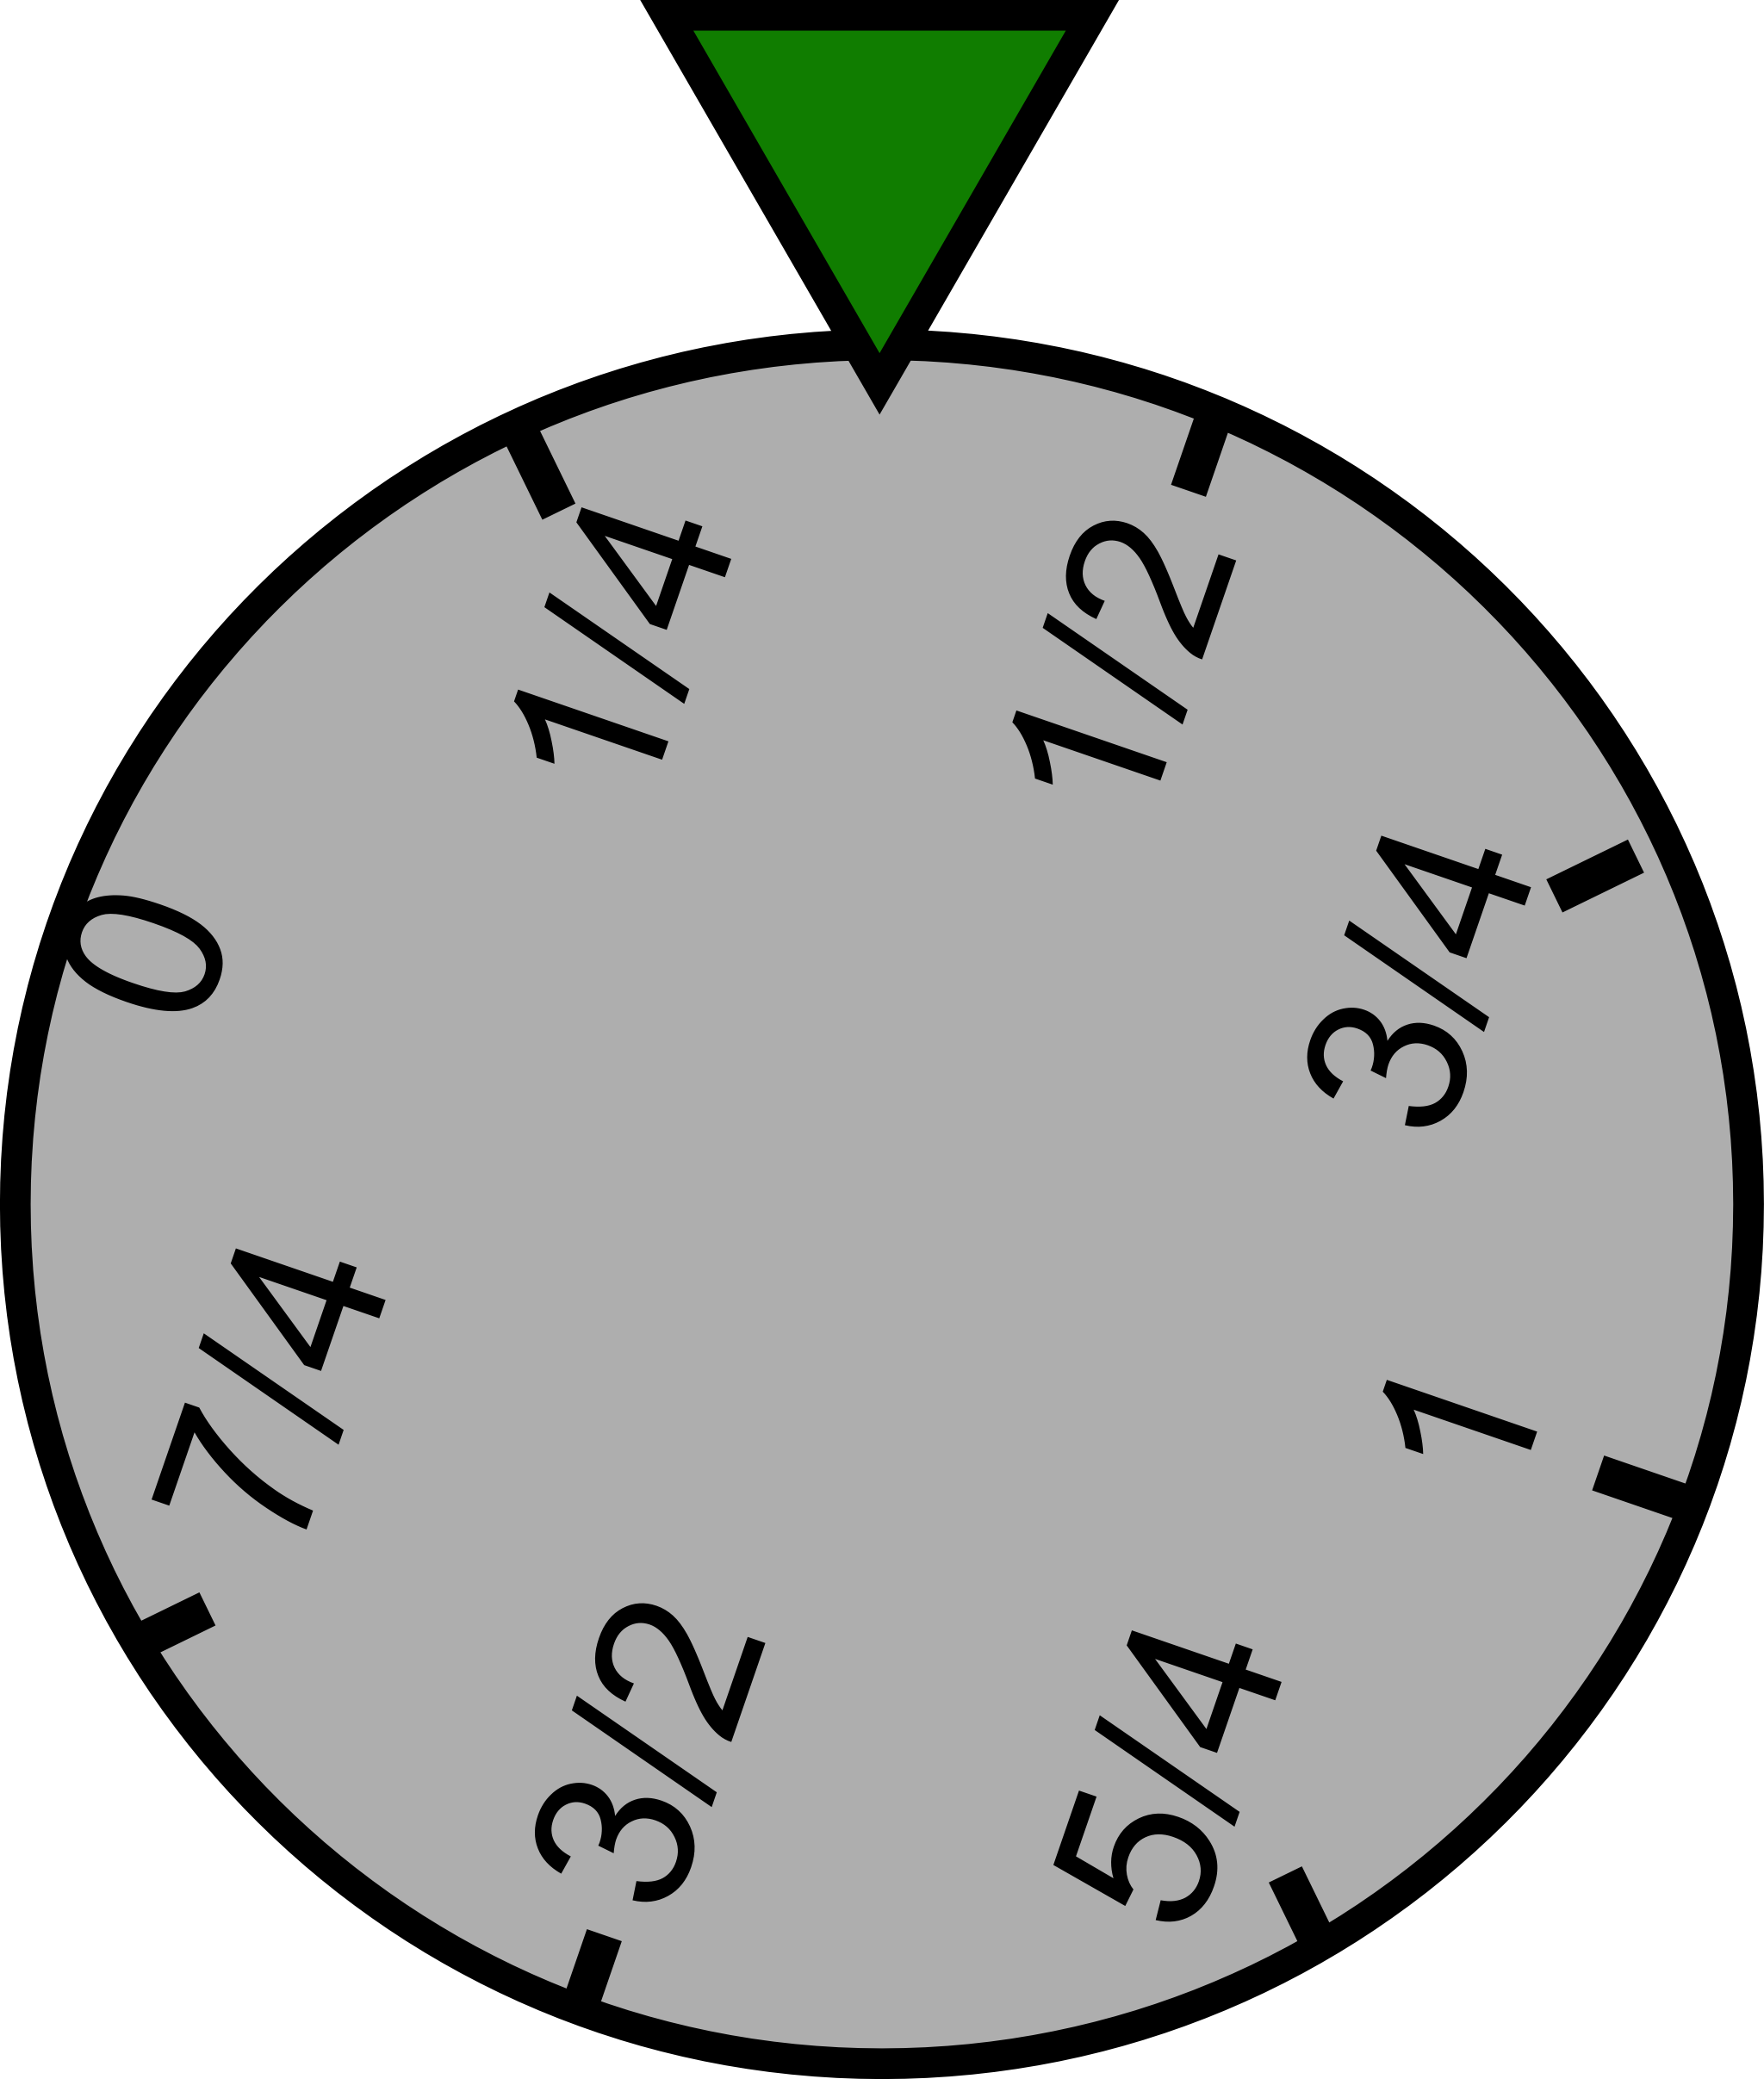
\includegraphics[width=3cm]{img/spinWheelRotated}}

  \only<3>{%
    What is the probability that $X$ is equal to $\frac{3}{8}$? \\
    $p\lp X=\frac{3}{8} \rp$
  }
  
\end{frame}

\begin{frame}{Ask a Different Question}

  I take a wheel that has a circumference of 2 and spin it. Let $X$ be
  the distance it turns.

  \includegraphics[width=3cm]{img/spinWheel}

  What is the probability that $X$ is between $\frac{1}{4}$ and  $\half$? \\
  $p\lp \frac{1}{4} \leq X \leq \half \rp$

  
\end{frame}

\begin{frame}
  \frametitle{Probability Distribution}

  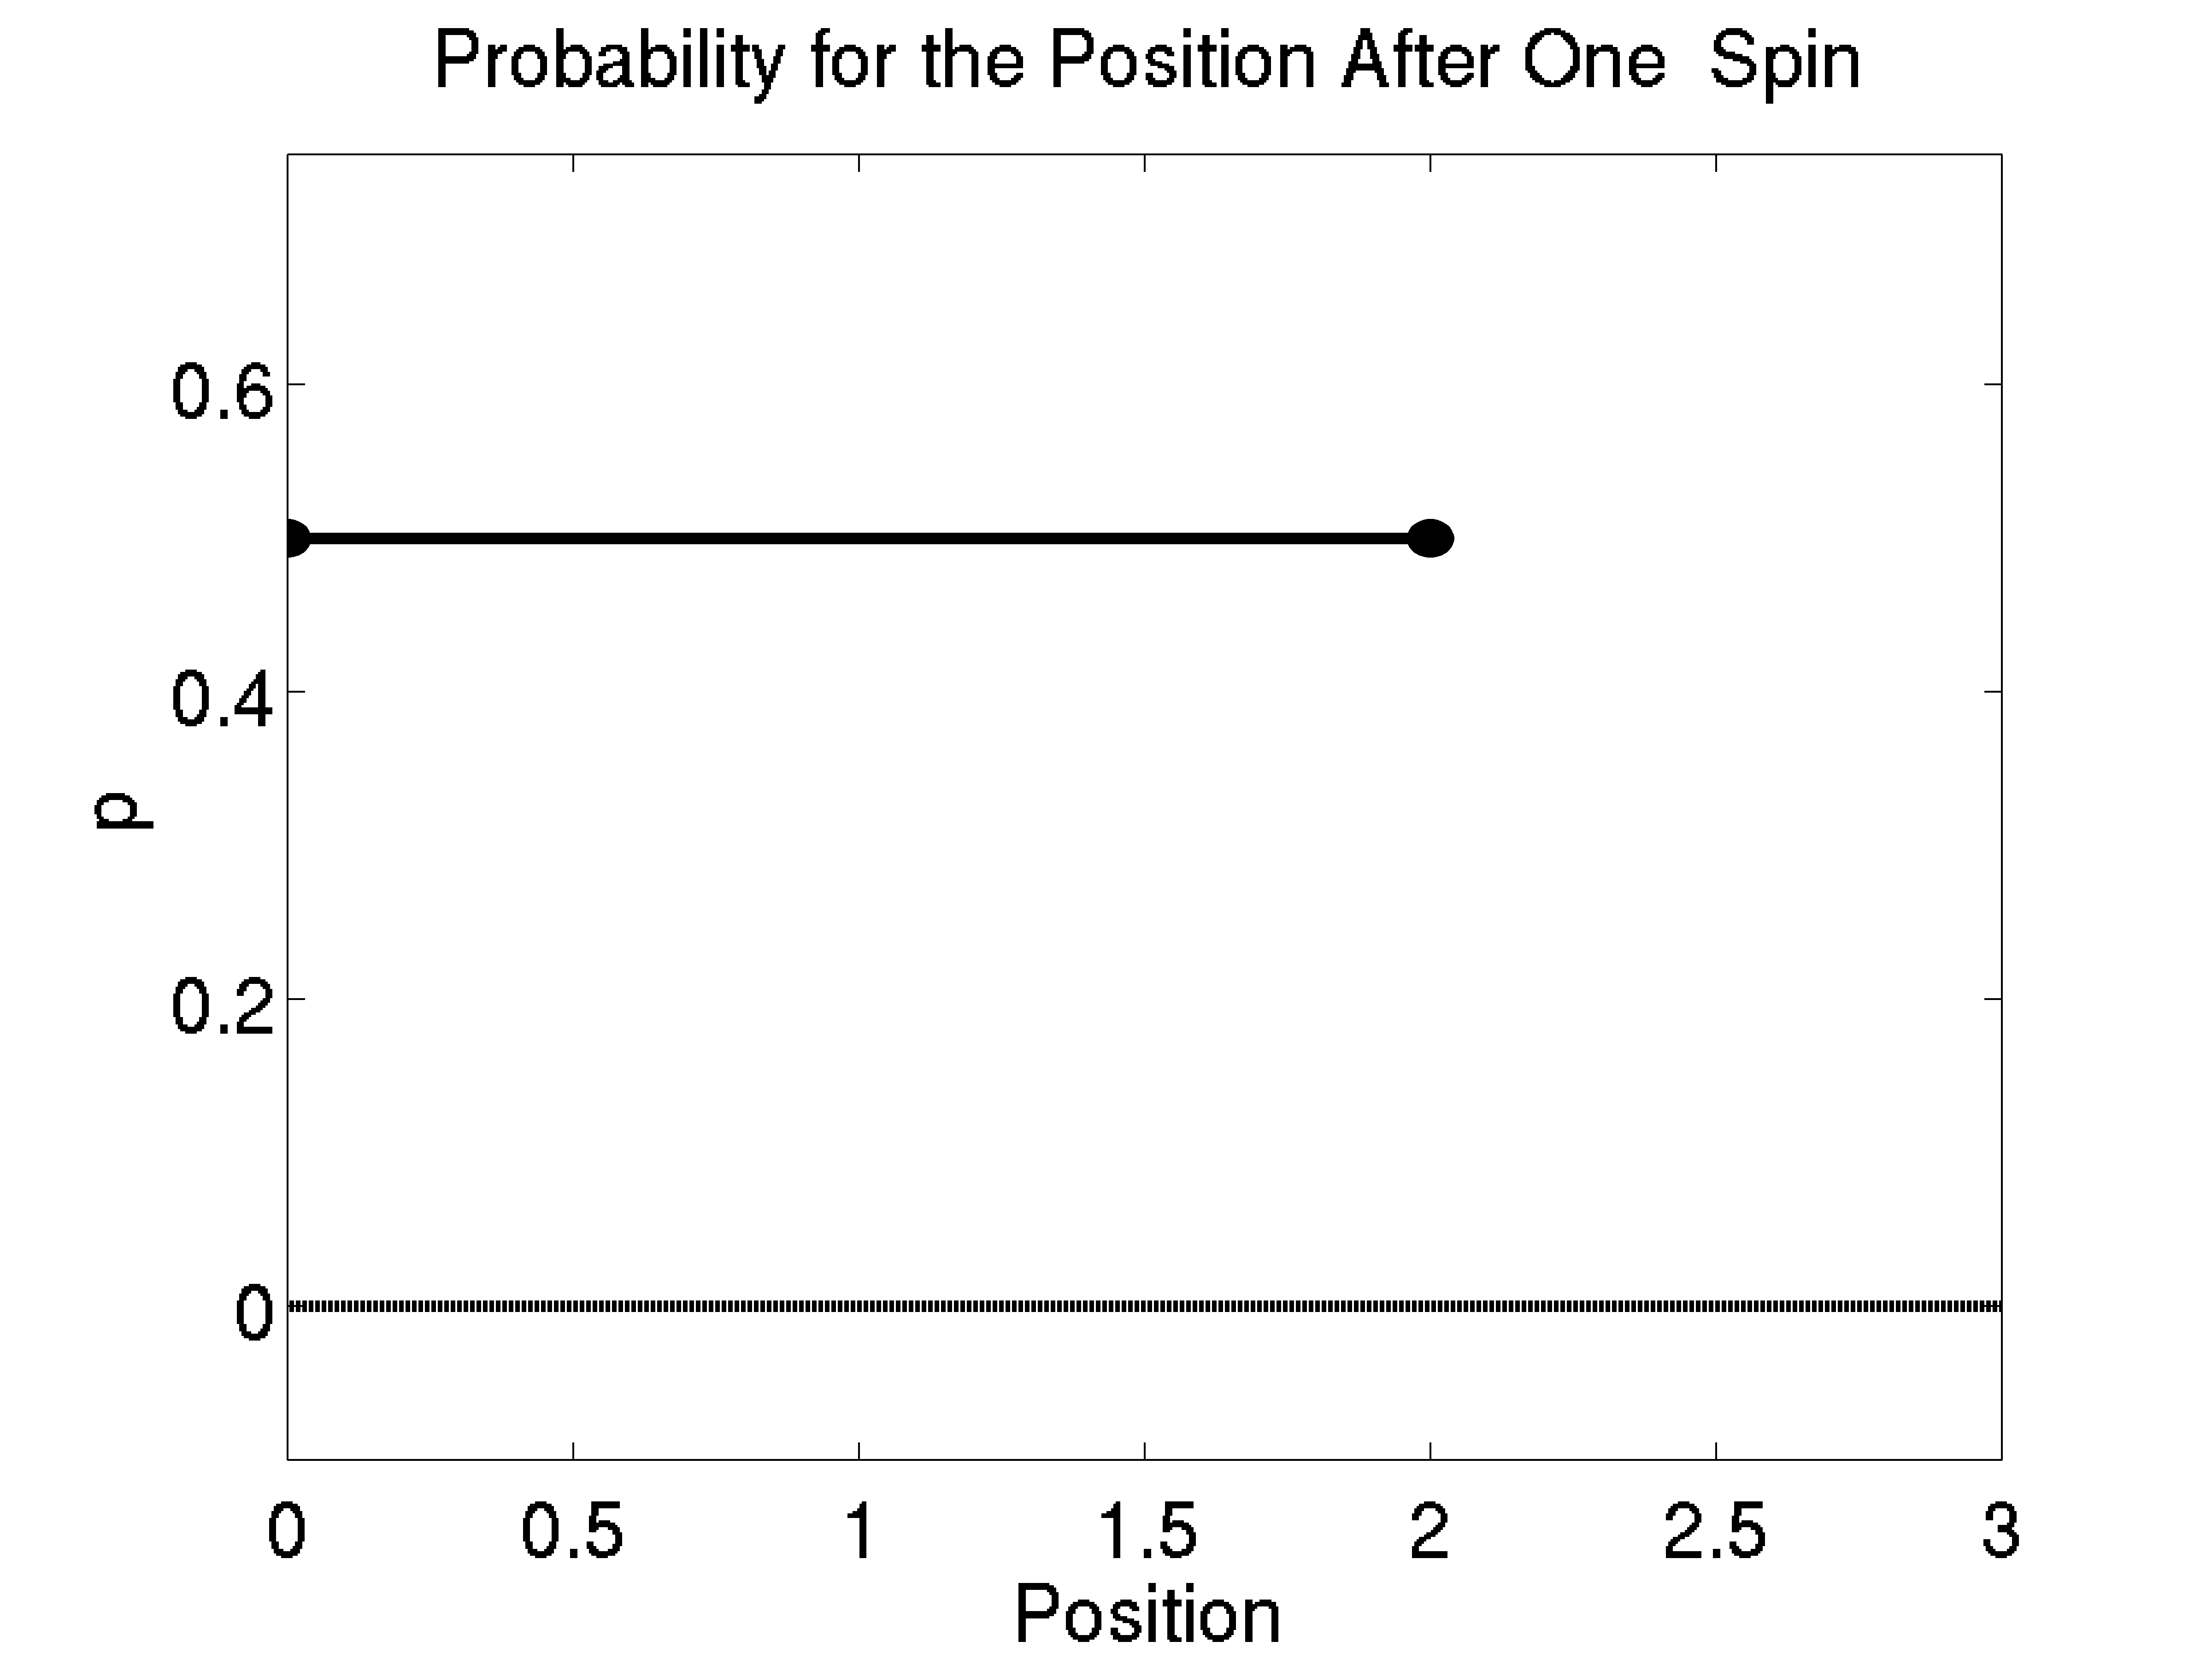
\includegraphics[width=5cm]{img/uniformDist}

  \begin{eqnarray*}
    f(x) & = & \left\{
      \begin{array}{l@{\hspace{2em}}rccccl}
      \half & 0 & \leq & x & \leq & 2 \\
      0 & \mathrm{otherwise}
    \end{array}
      \right.
  \end{eqnarray*}

\end{frame}


\begin{frame}
  \frametitle{Probability Distribution}

  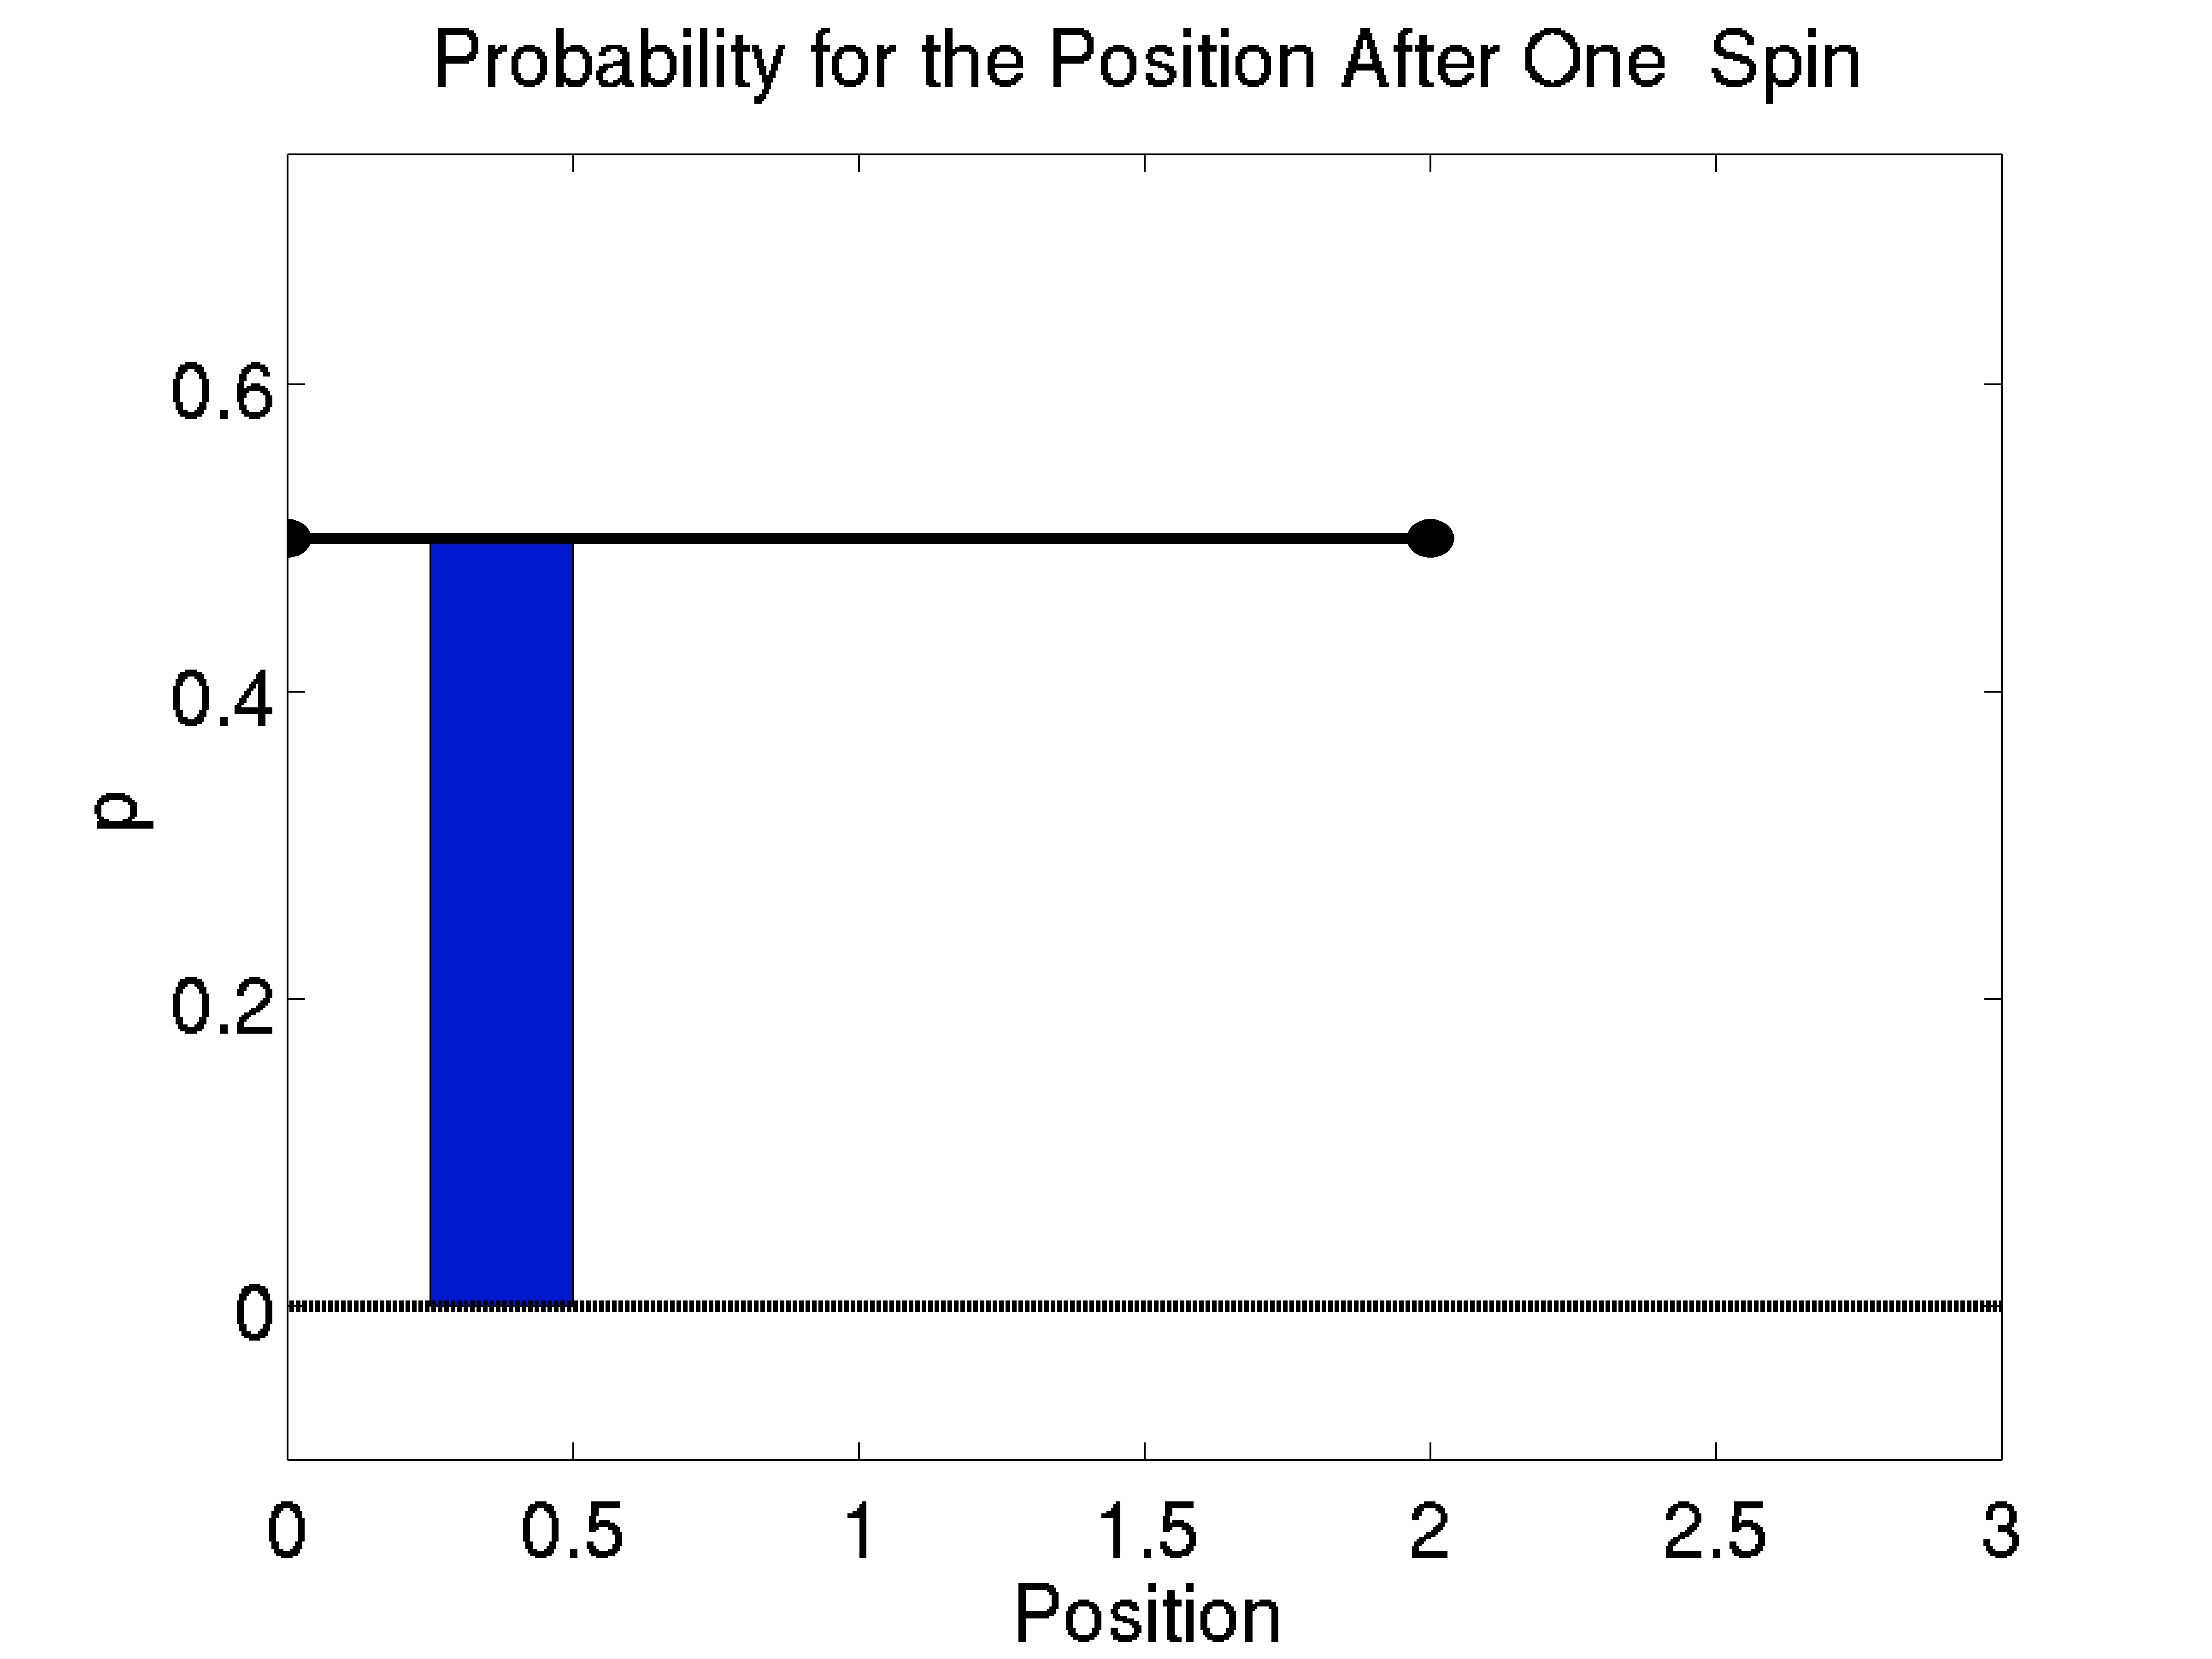
\includegraphics[width=5cm]{img/uniformDistArea}

  \begin{eqnarray*}
    p\lp\frac{1}{4} \leq X \leq \half \rp.
  \end{eqnarray*}

\end{frame}


\begin{frame}{The Probability Density Function}

  \begin{definition}
    A probability density function is a function that satisfies the
    folllowing properties:
    \begin{enumerate}
    \item The area under the function is one.
    \item The function is always greater than or equal to zero.
    \end{enumerate}
  \end{definition}

  In the previous example the probability density function was
  \begin{eqnarray*}
    f(x) & = & \left\{
      \begin{array}{l@{\hspace{2em}}rccccl}
      \half & 0 & \leq & x & \leq & 2 \\
      0 & \mathrm{otherwise}
    \end{array}
      \right.
  \end{eqnarray*}

  
\end{frame}

\begin{frame}{Example}
  A bus may show up to a stop at any time between 1:00pm and 1:15pm
  with a uniform probability distribution. What is the probability
  that it will show up before 1:05pm?
\end{frame}

\subsection{The Normal Distribution}

\begin{frame}{The Normal Distribution}

  \only<1>{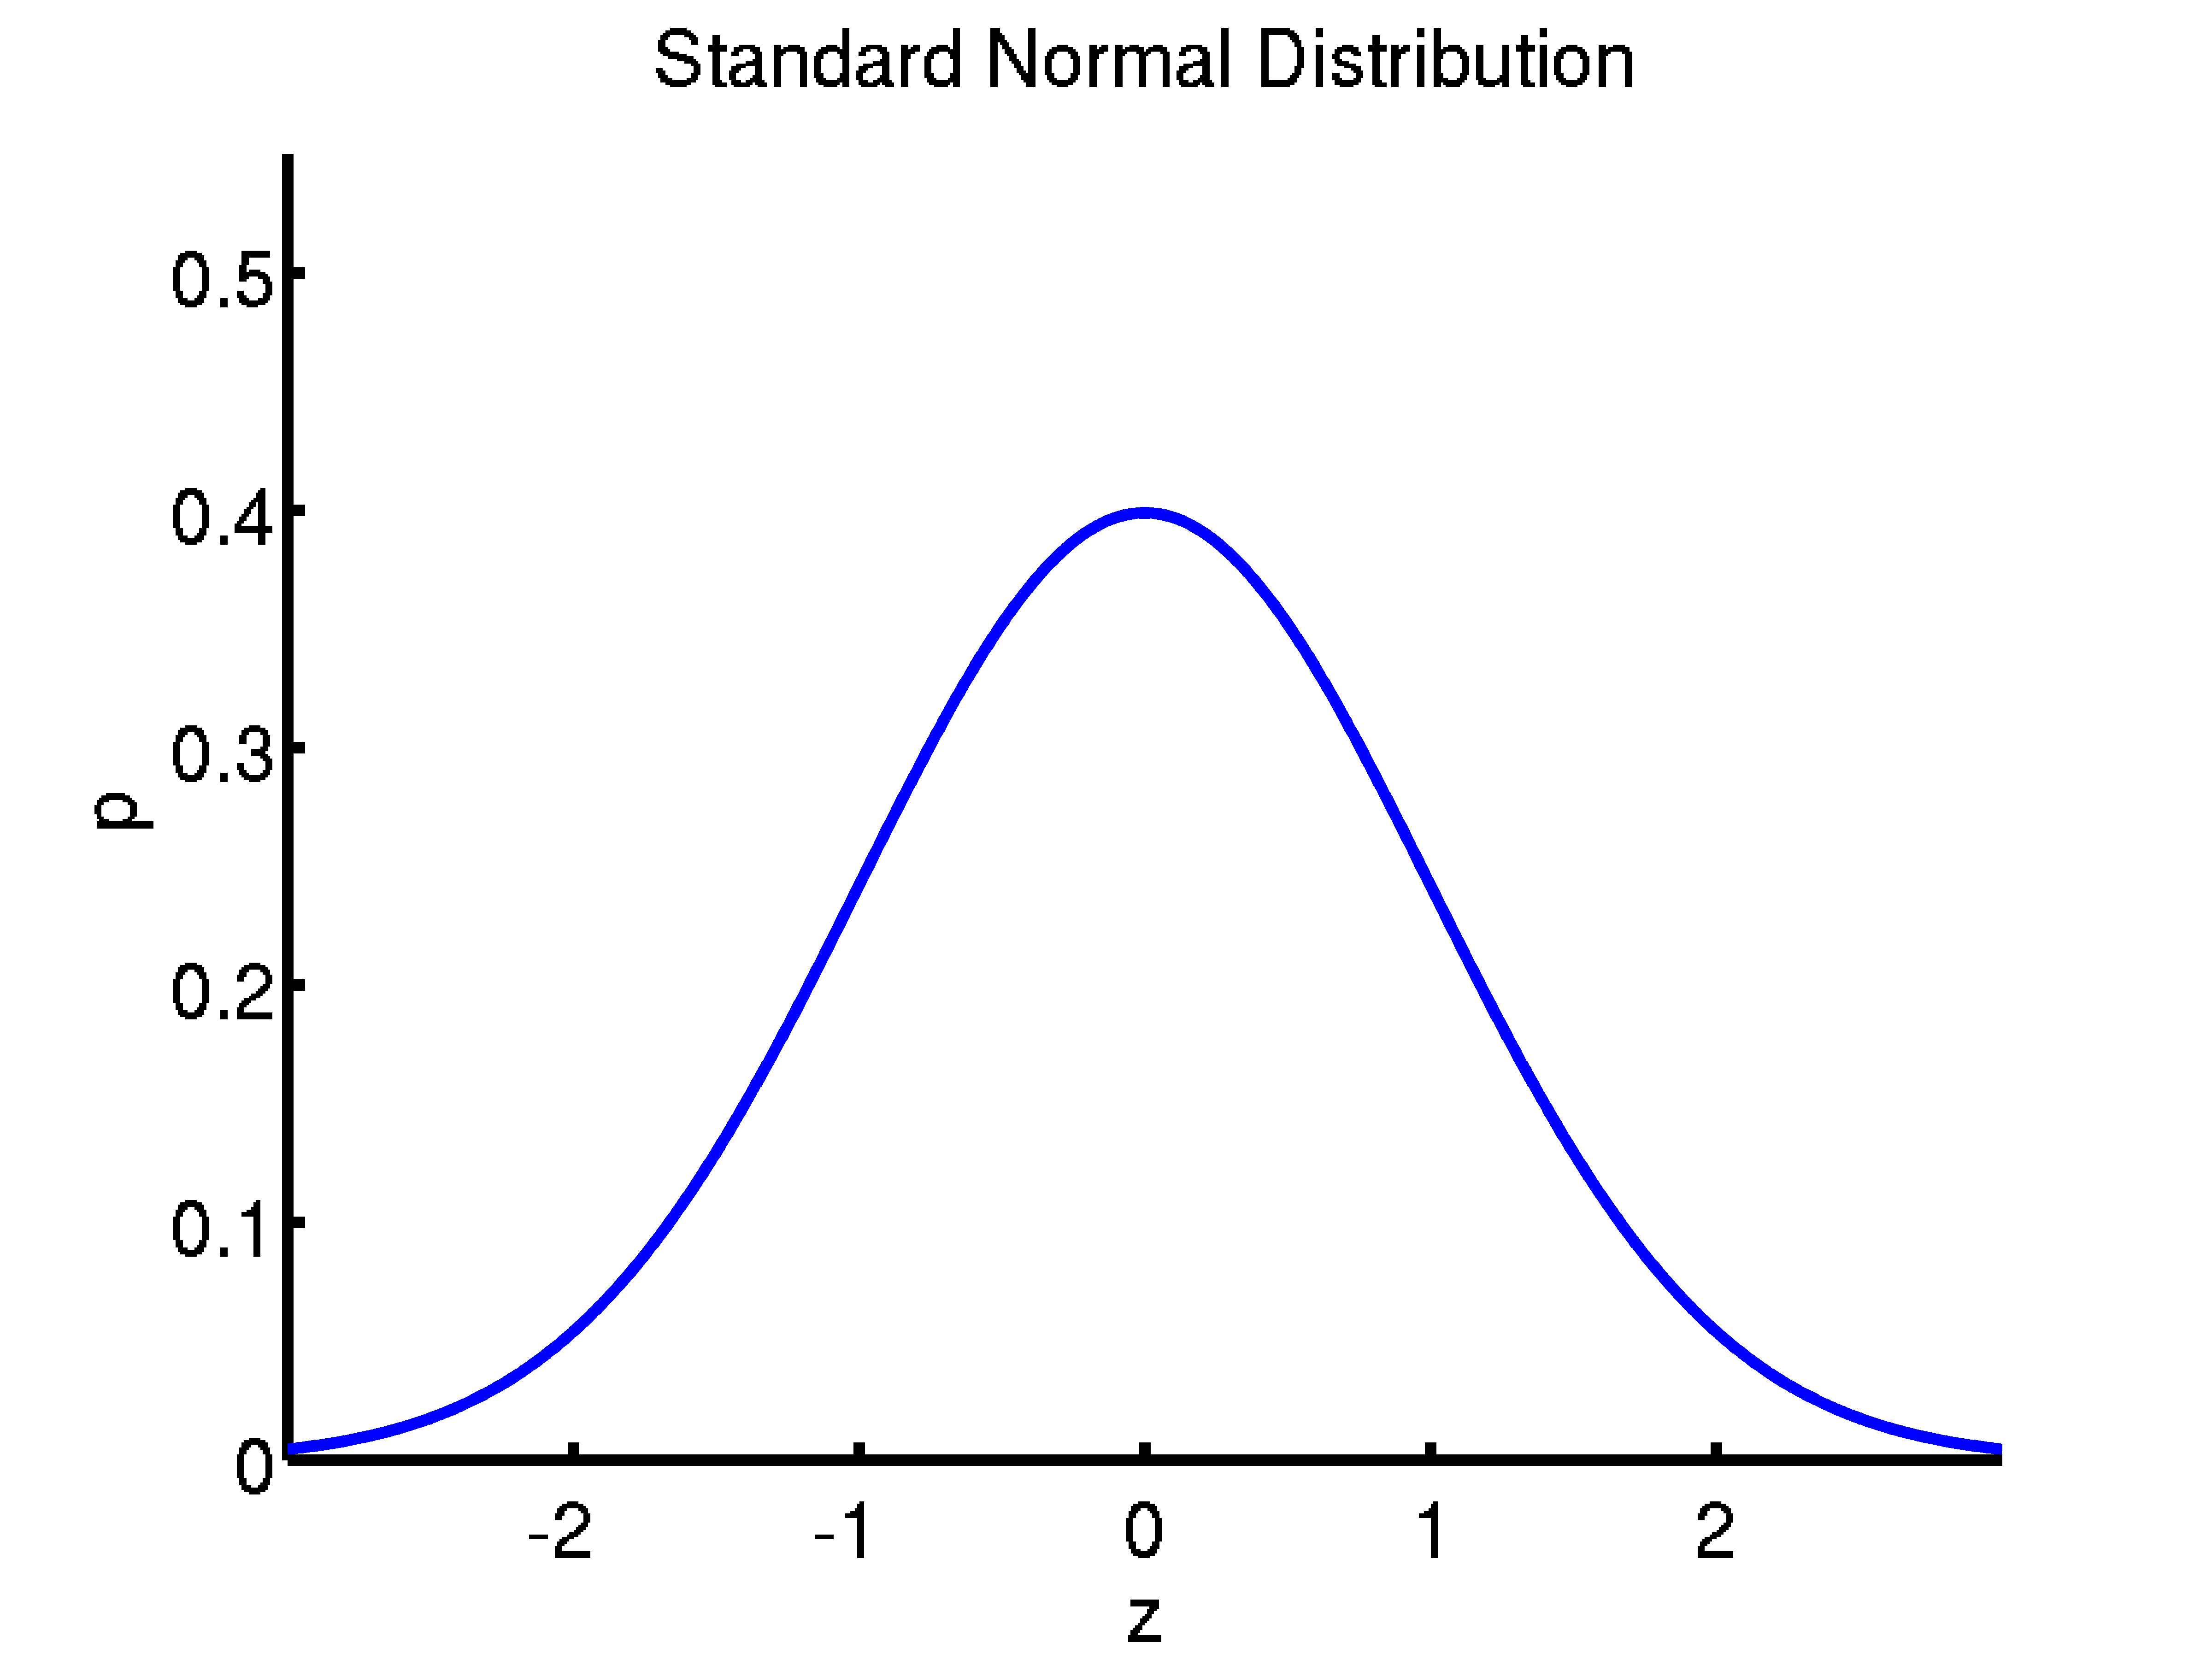
\includegraphics[width=5cm]{img/standardNormal}}
  \only<2>{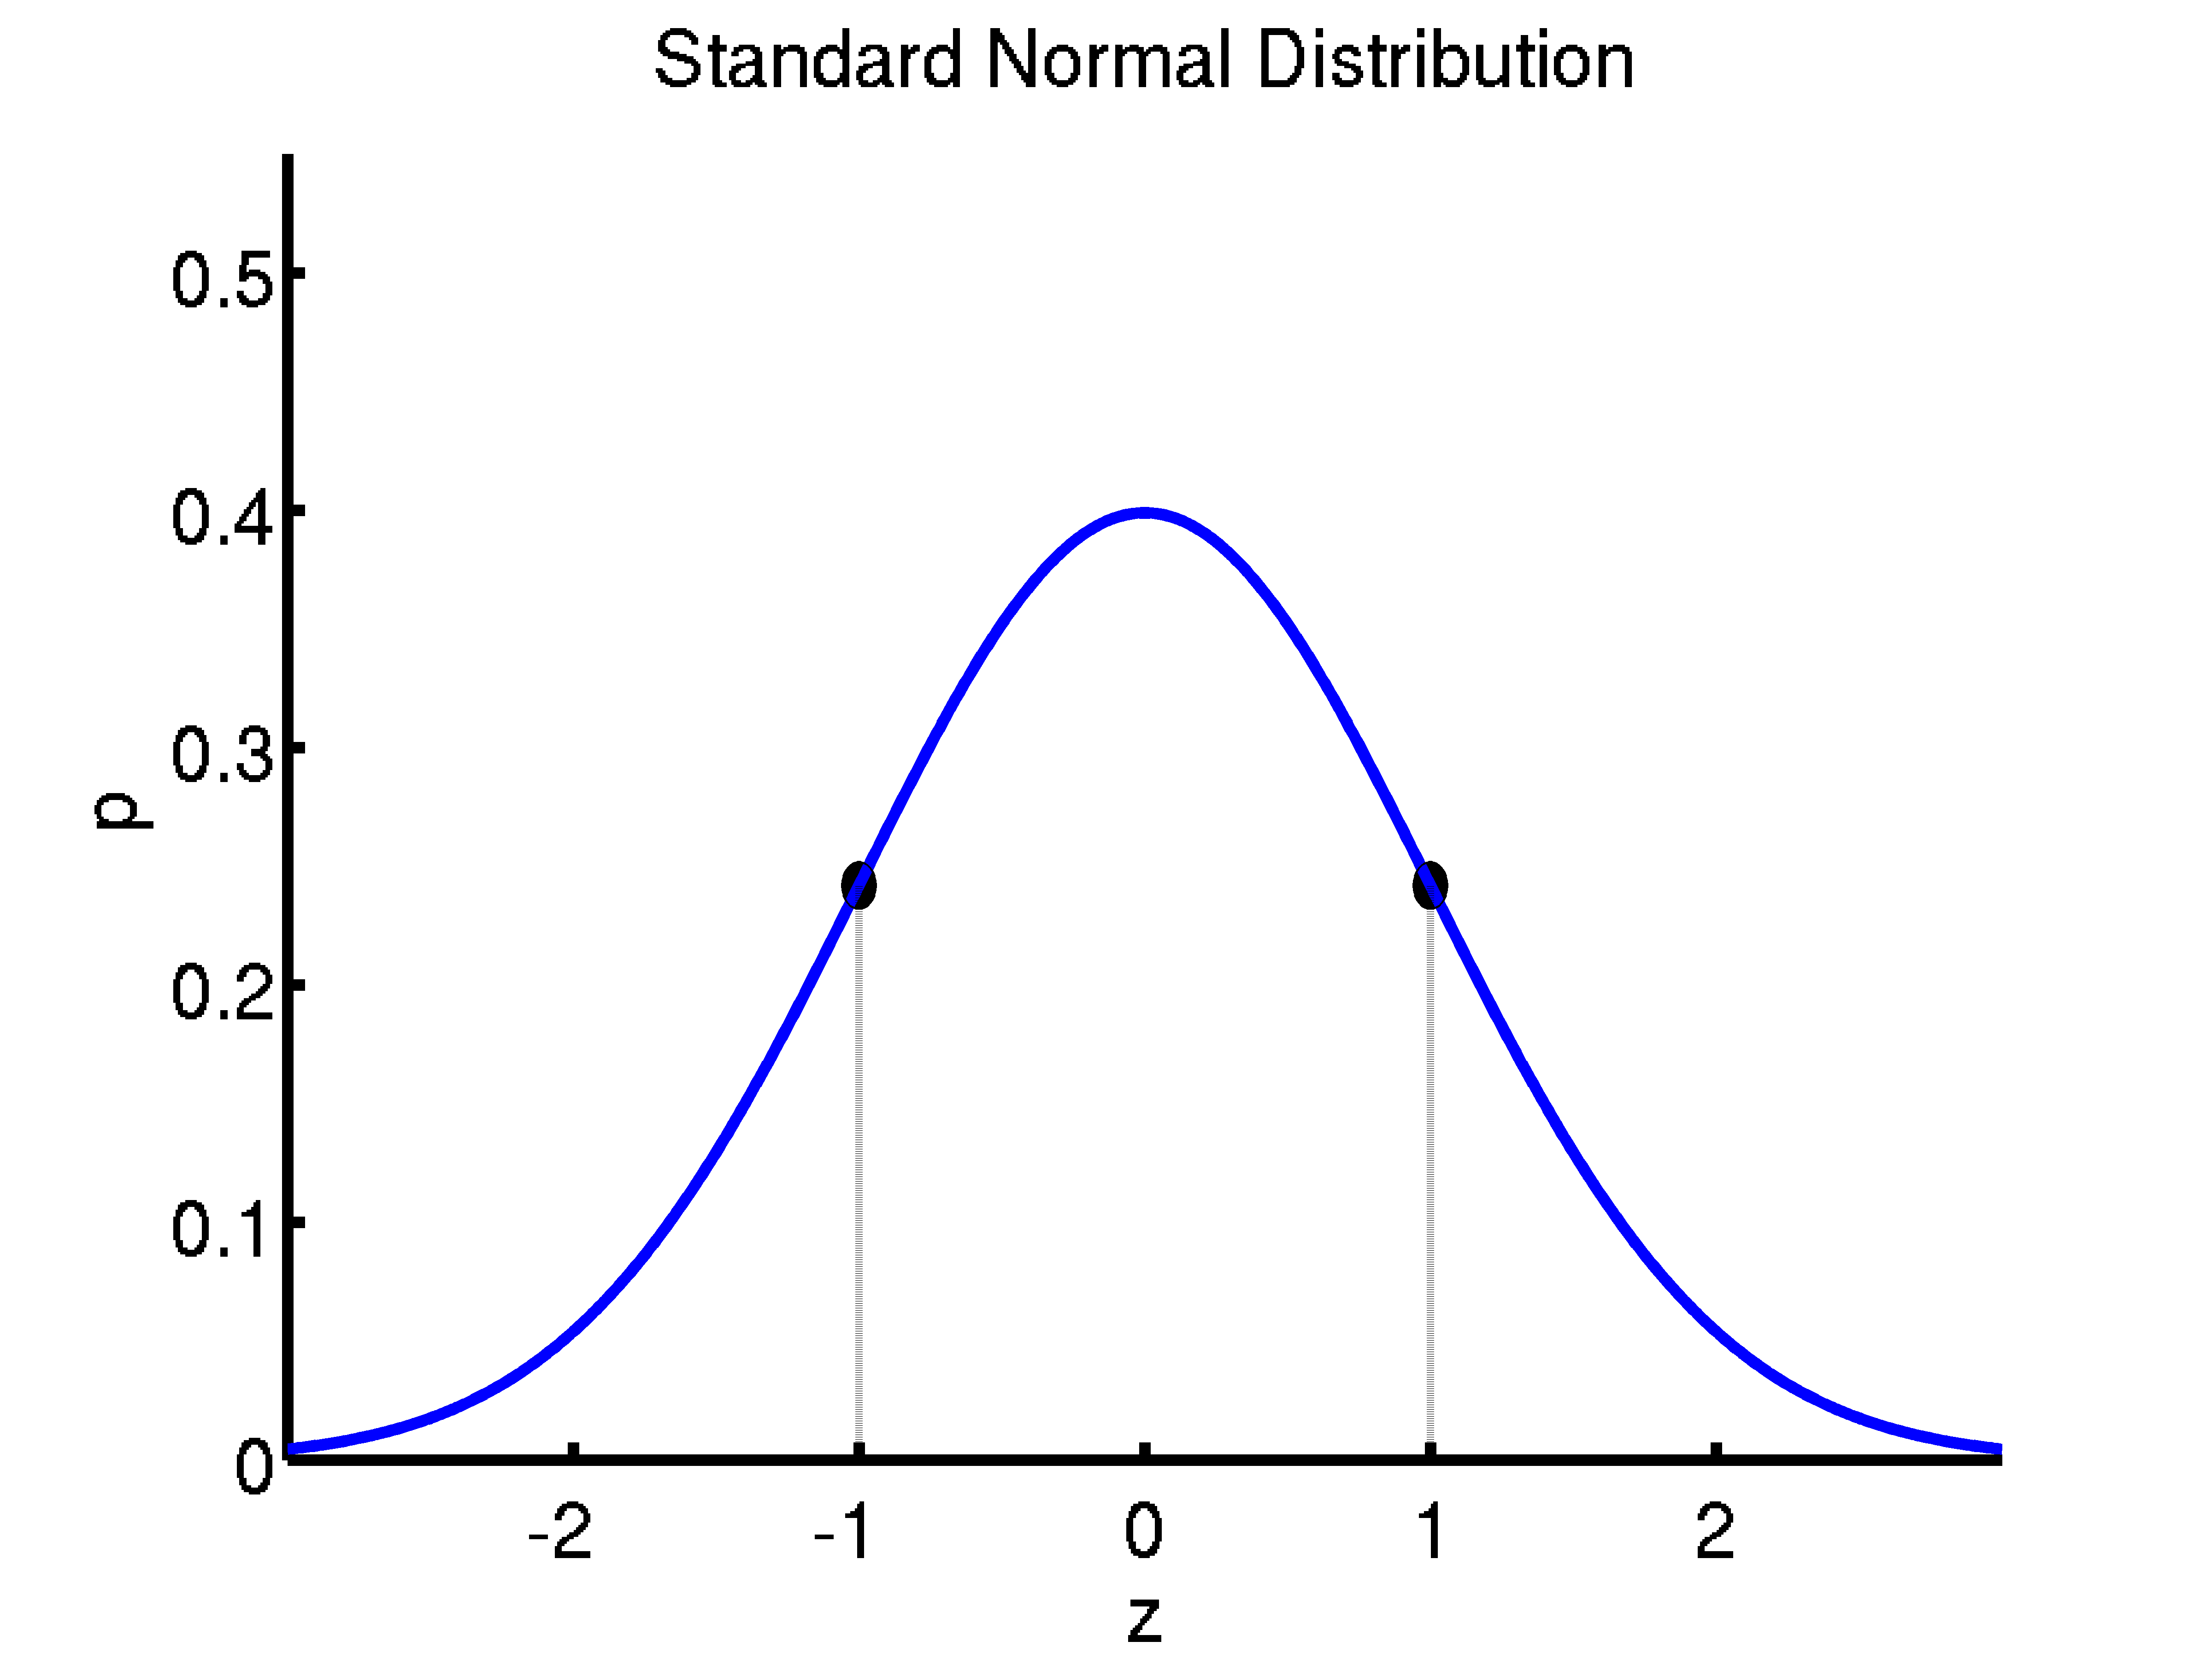
\includegraphics[width=5cm]{img/standardNormalInflection}}

  \begin{eqnarray*}
    f(z) & = & \frac{1}{\sqrt{2\pi}} e^{-z^2/2}.
  \end{eqnarray*}
  
\end{frame}

\begin{frame}{Probability and Area}

  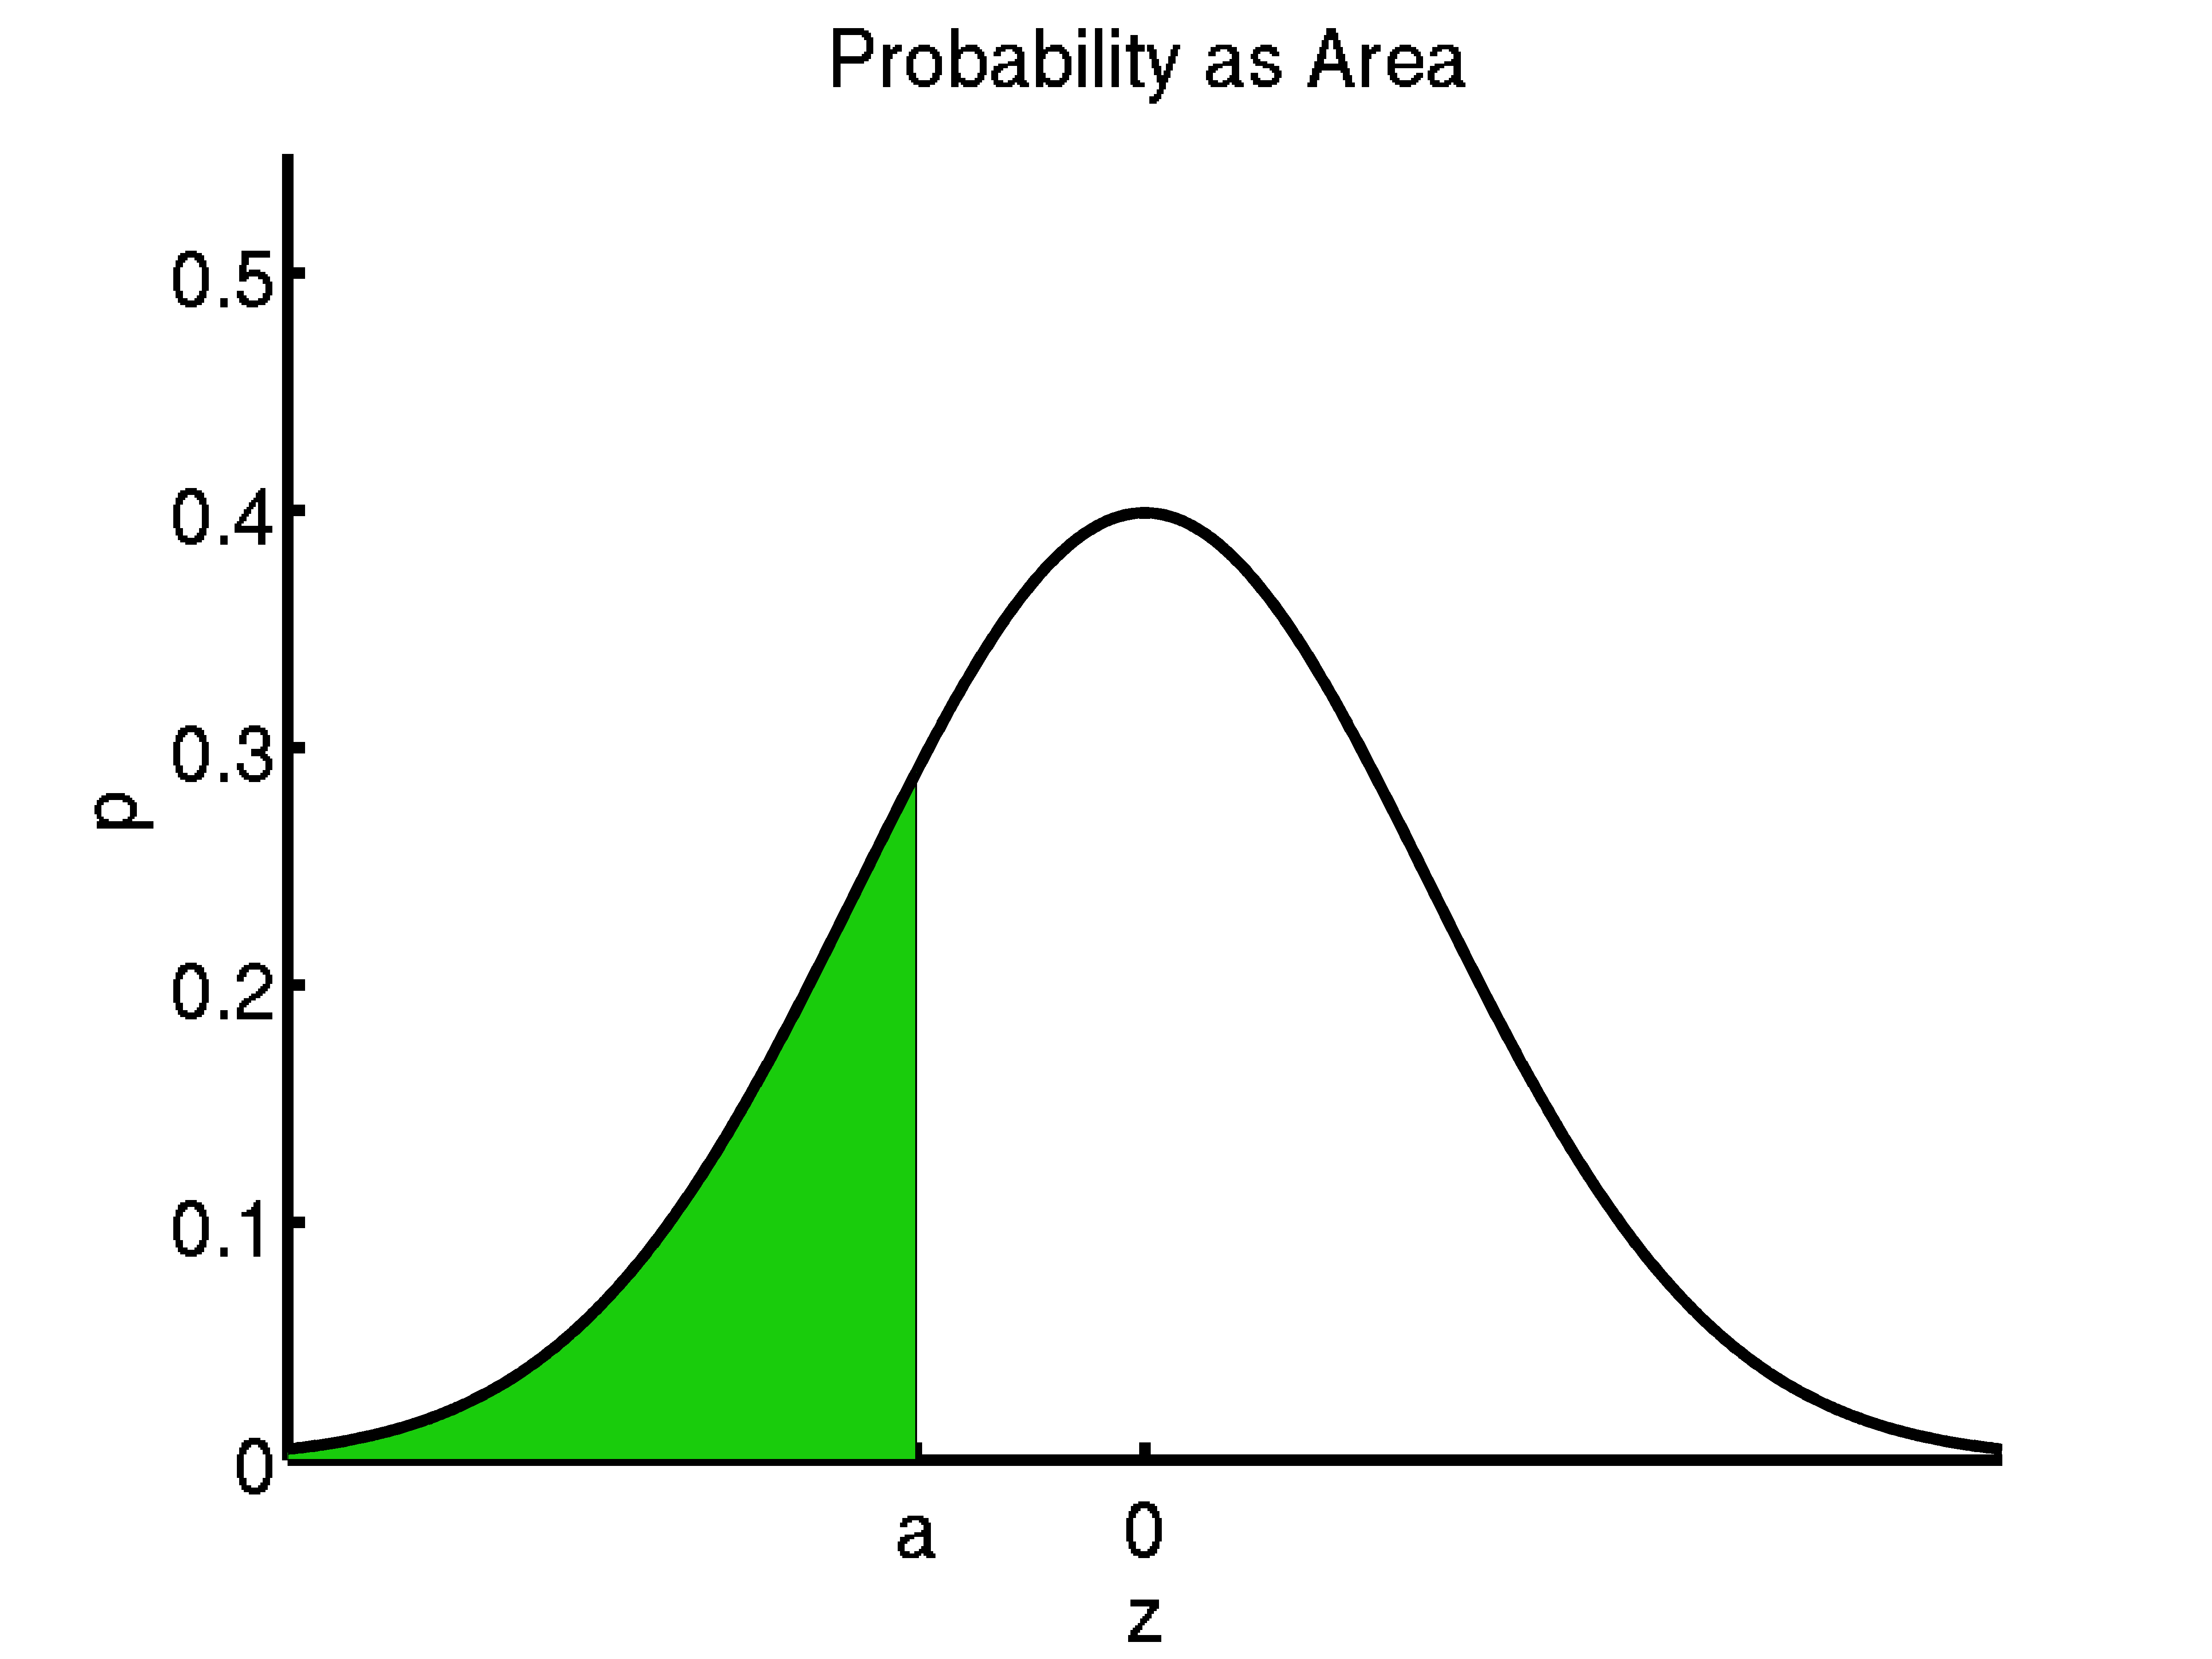
\includegraphics[width=5cm]{img/standardNormalArea}

  \begin{eqnarray*}
    p(X \leq a) 
  \end{eqnarray*}
  
\end{frame}


\begin{frame}{Probability and Area}

  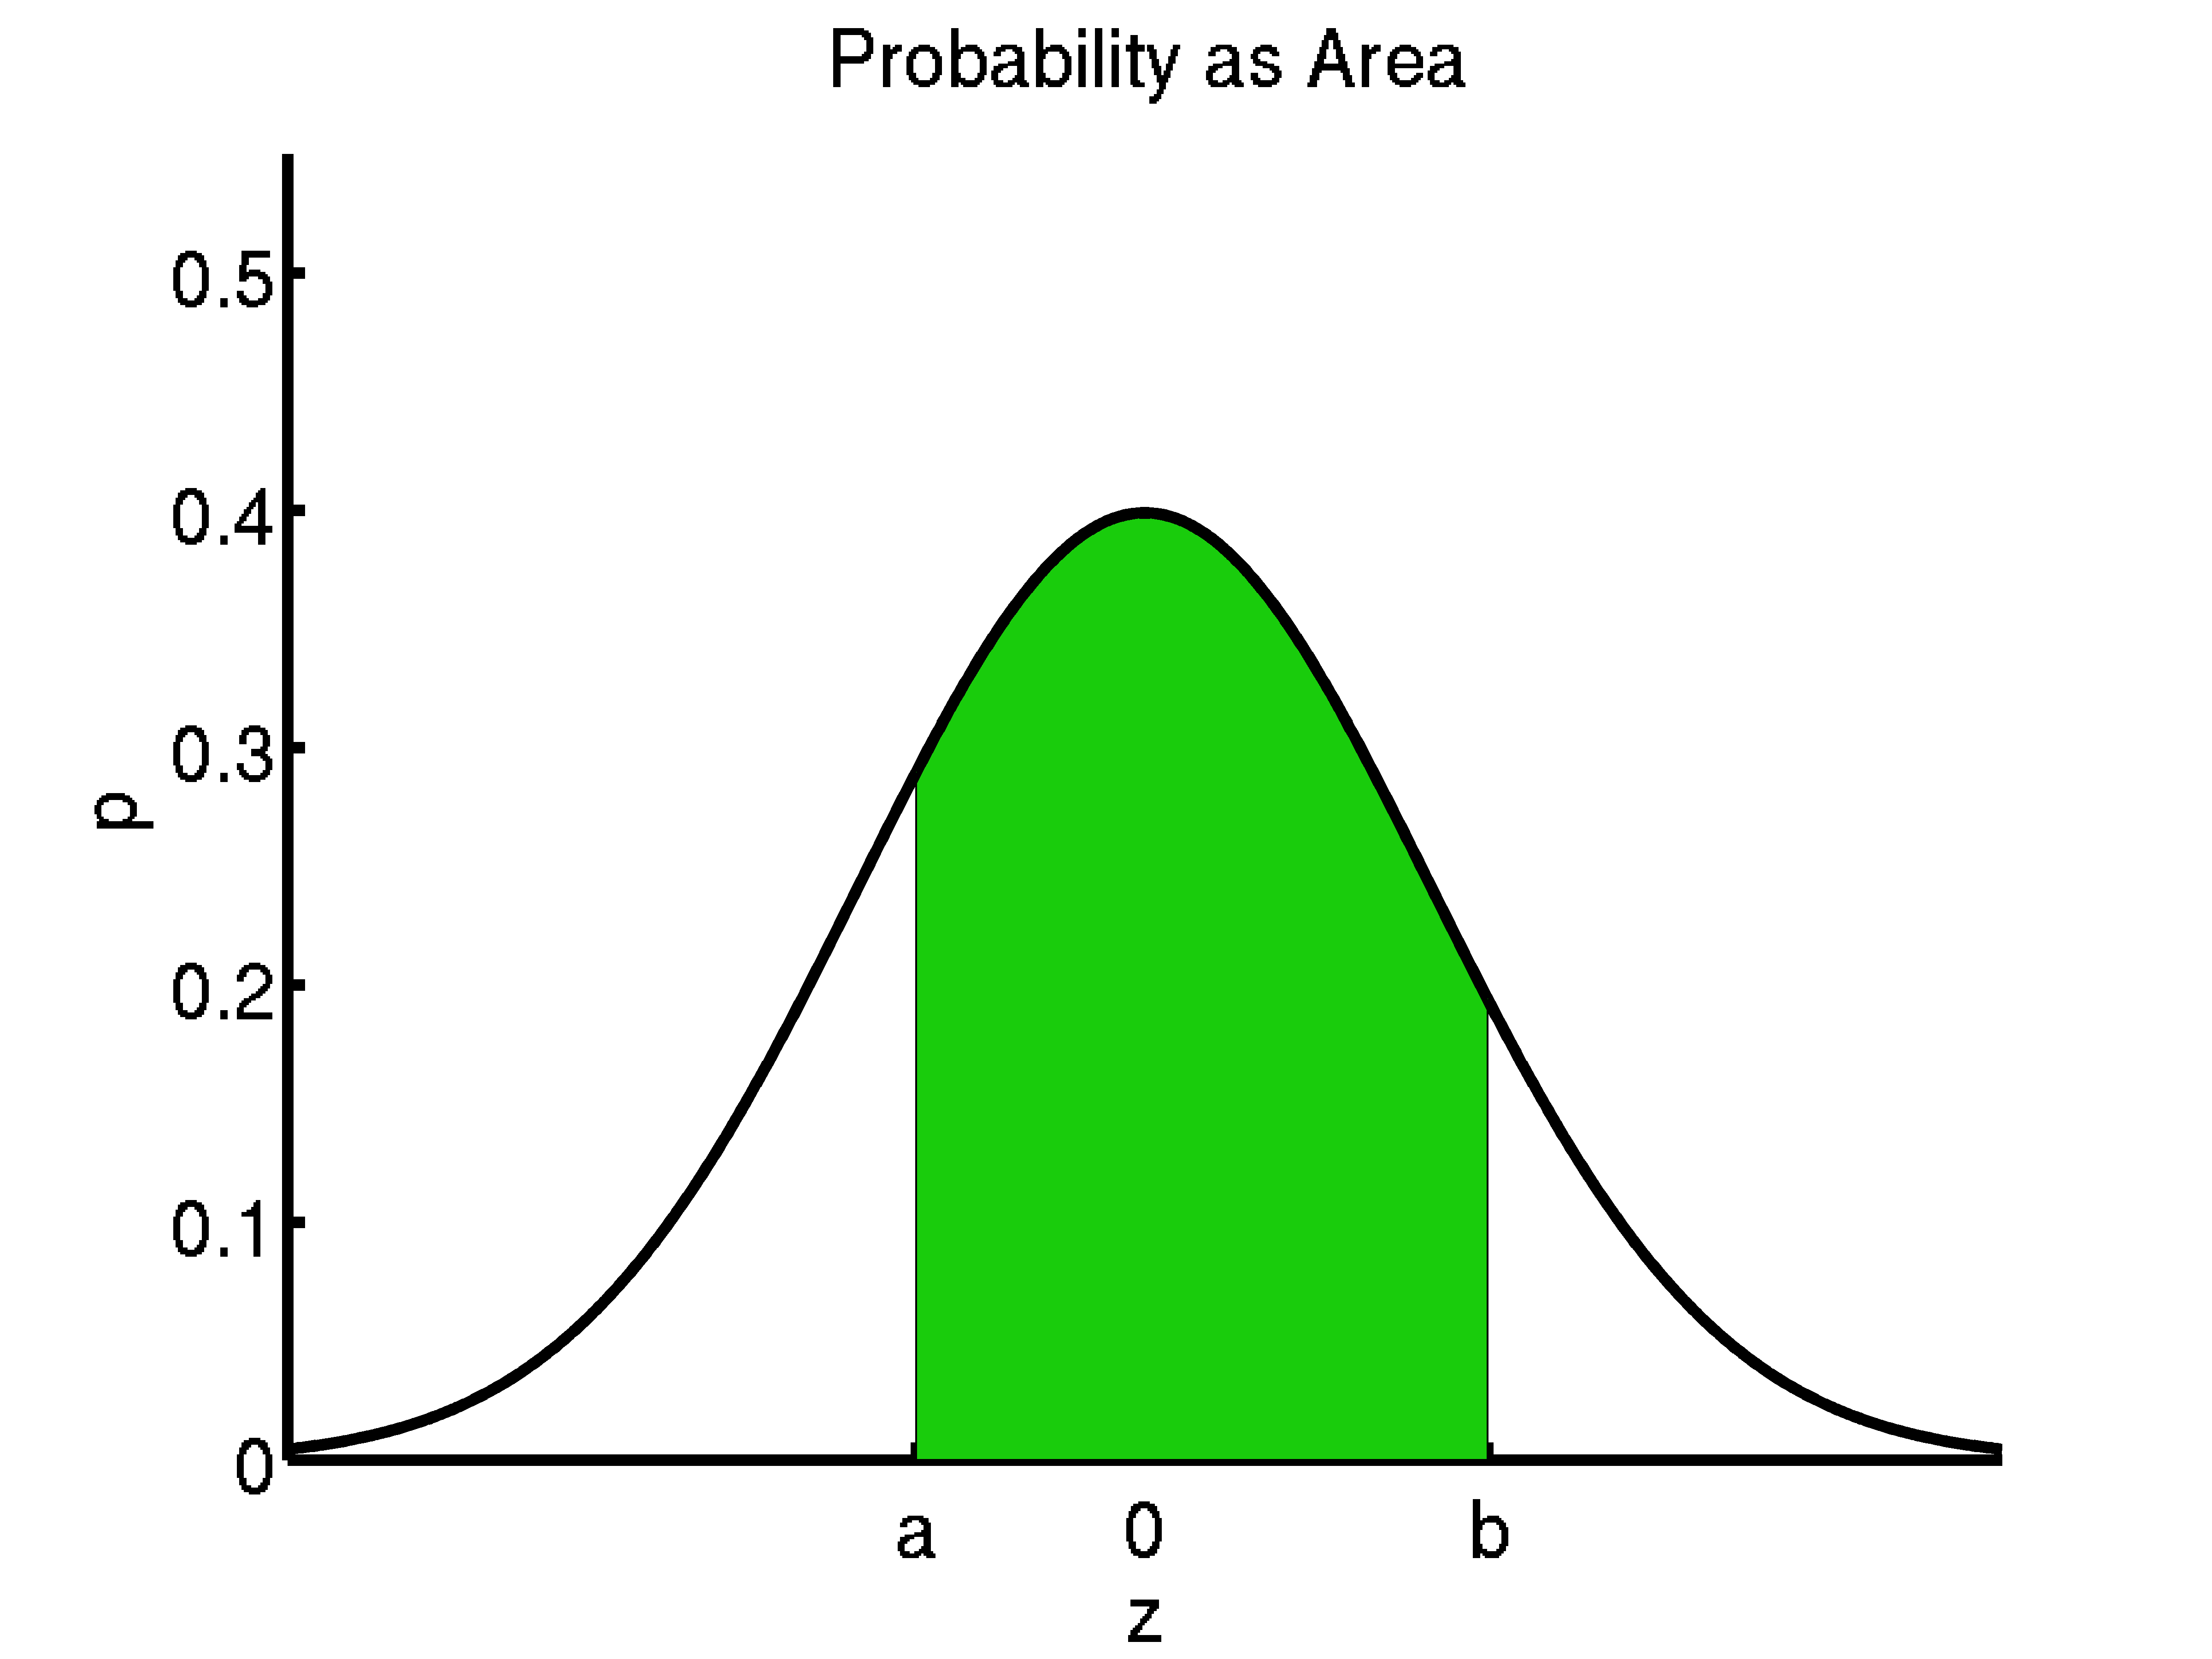
\includegraphics[width=5cm]{img/standardNormalAreaBoth}

  \begin{eqnarray*}
    p(a \leq X \leq b) 
  \end{eqnarray*}
  
\end{frame}

\begin{frame}{Probability and Area}

  \begin{tabular}{lcr}
  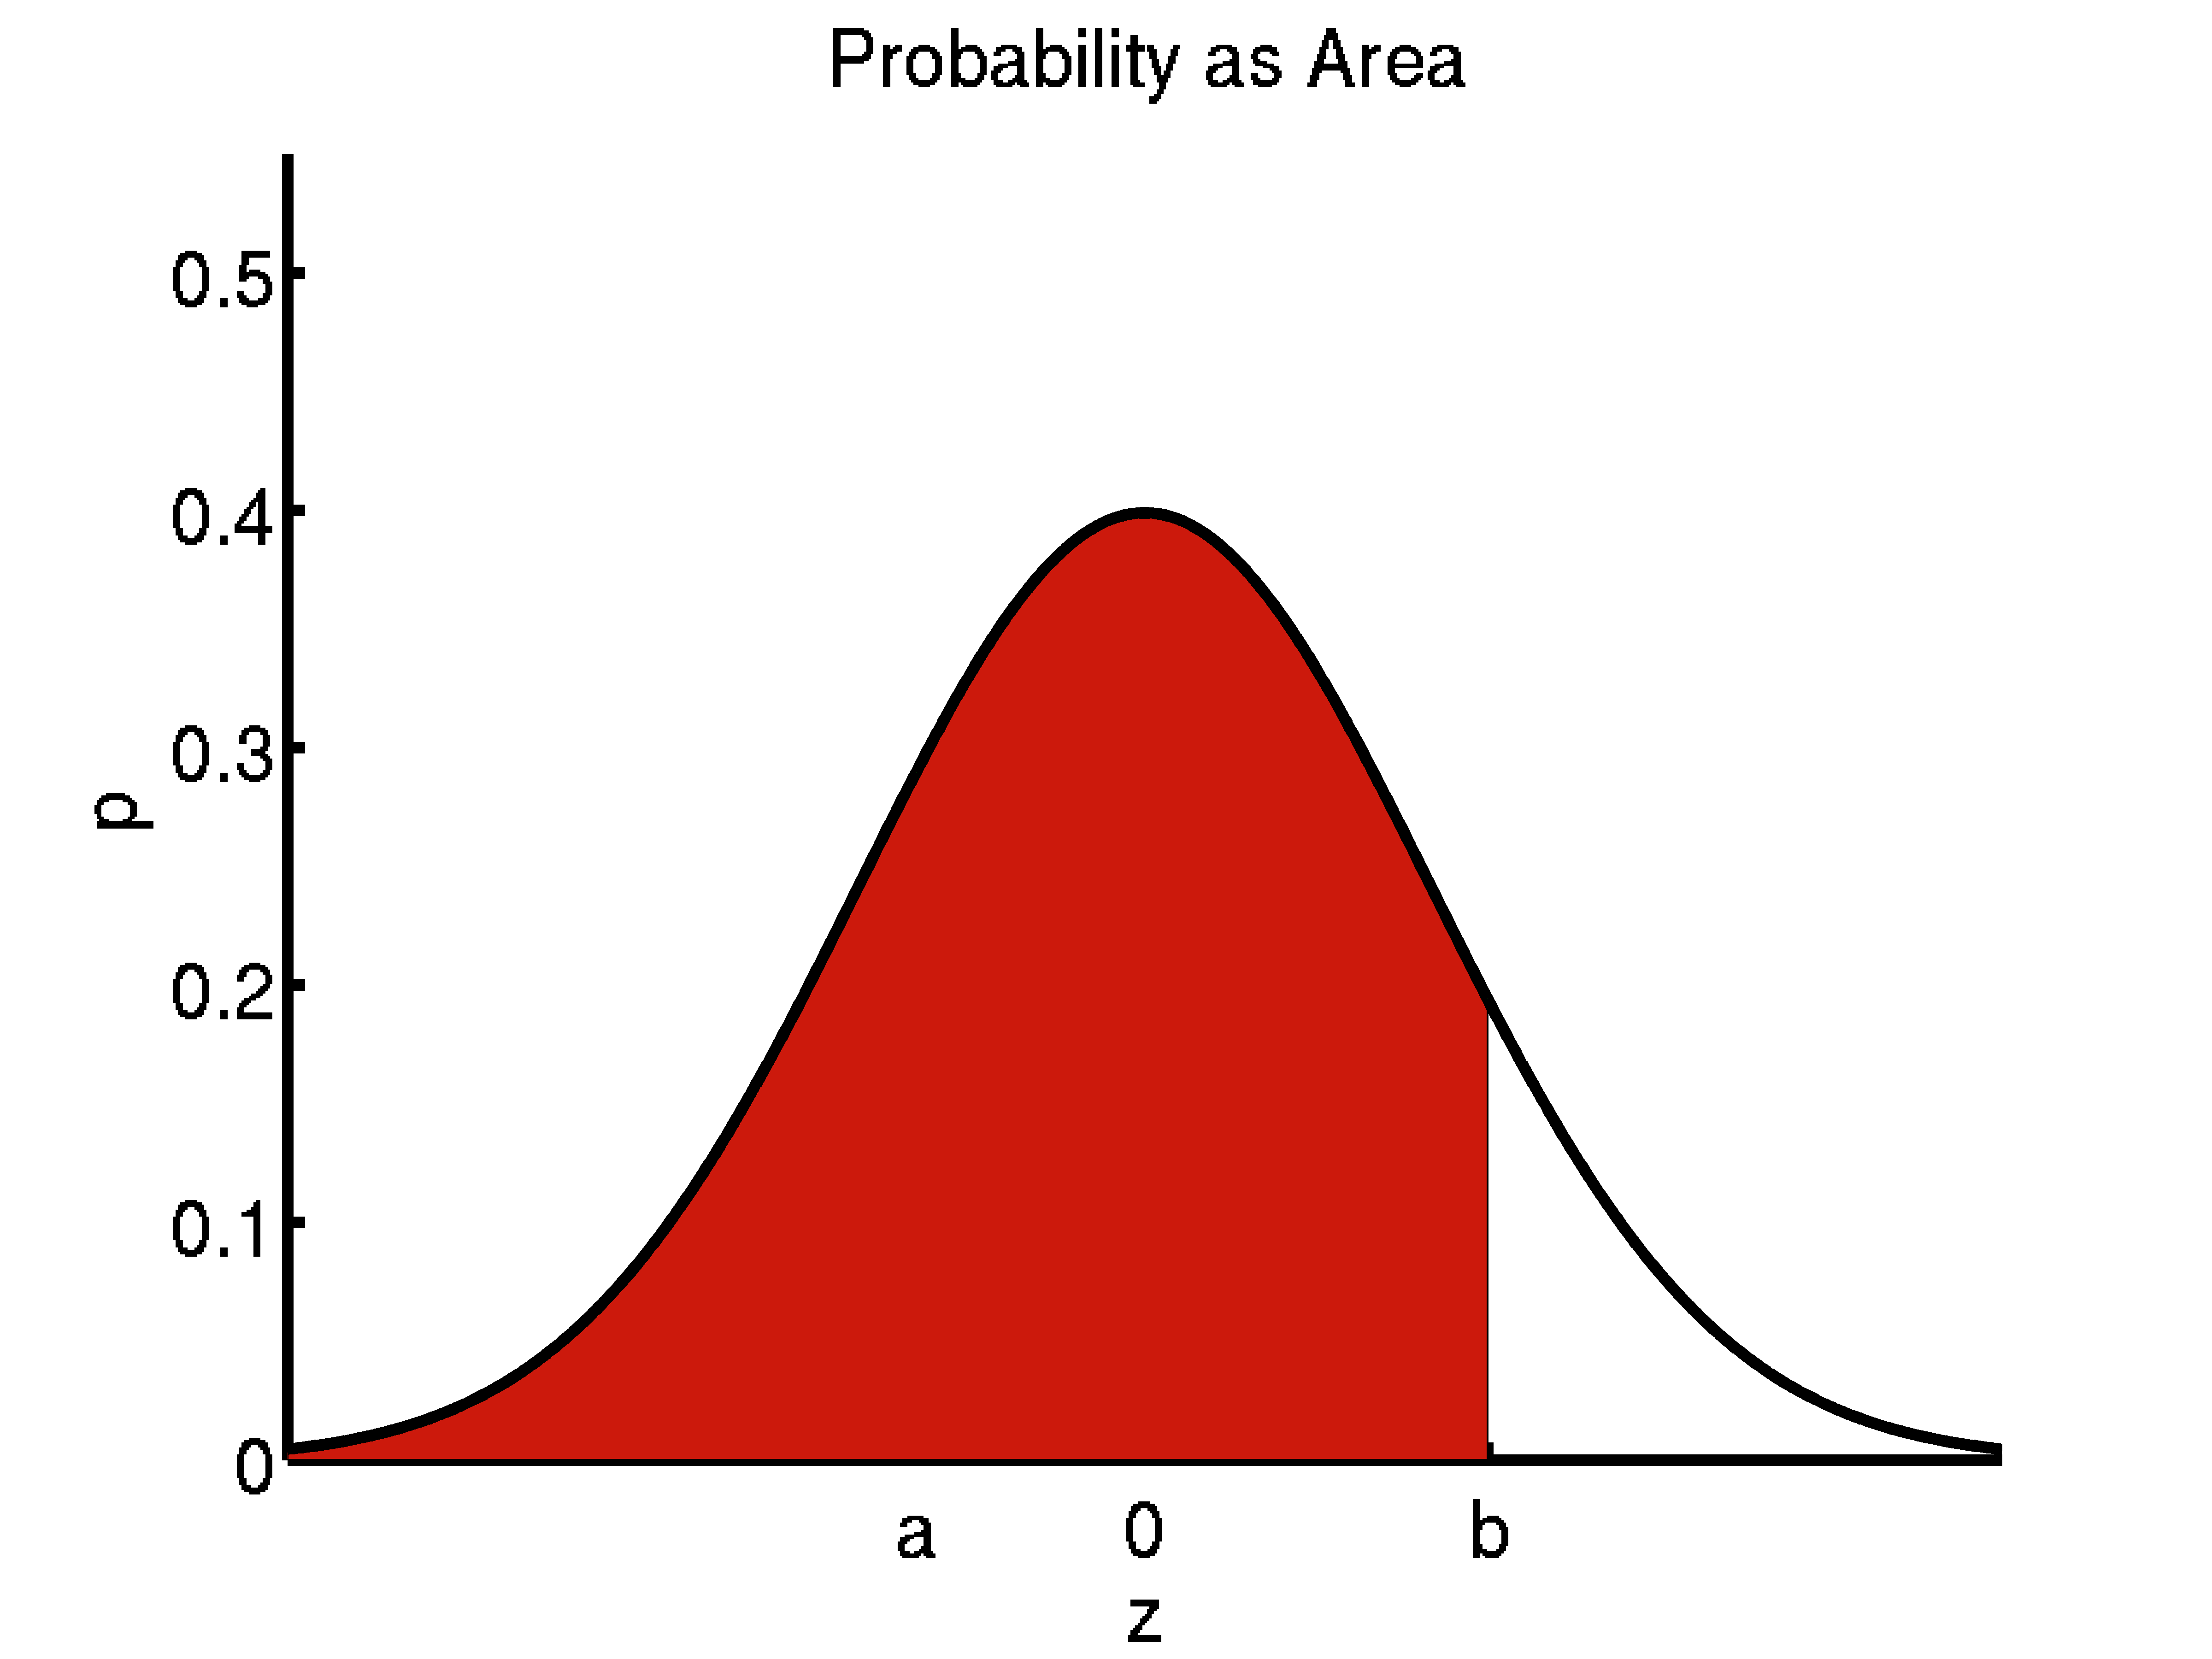
\includegraphics[width=3.5cm]{img/standardNormalRightArea} & - &
  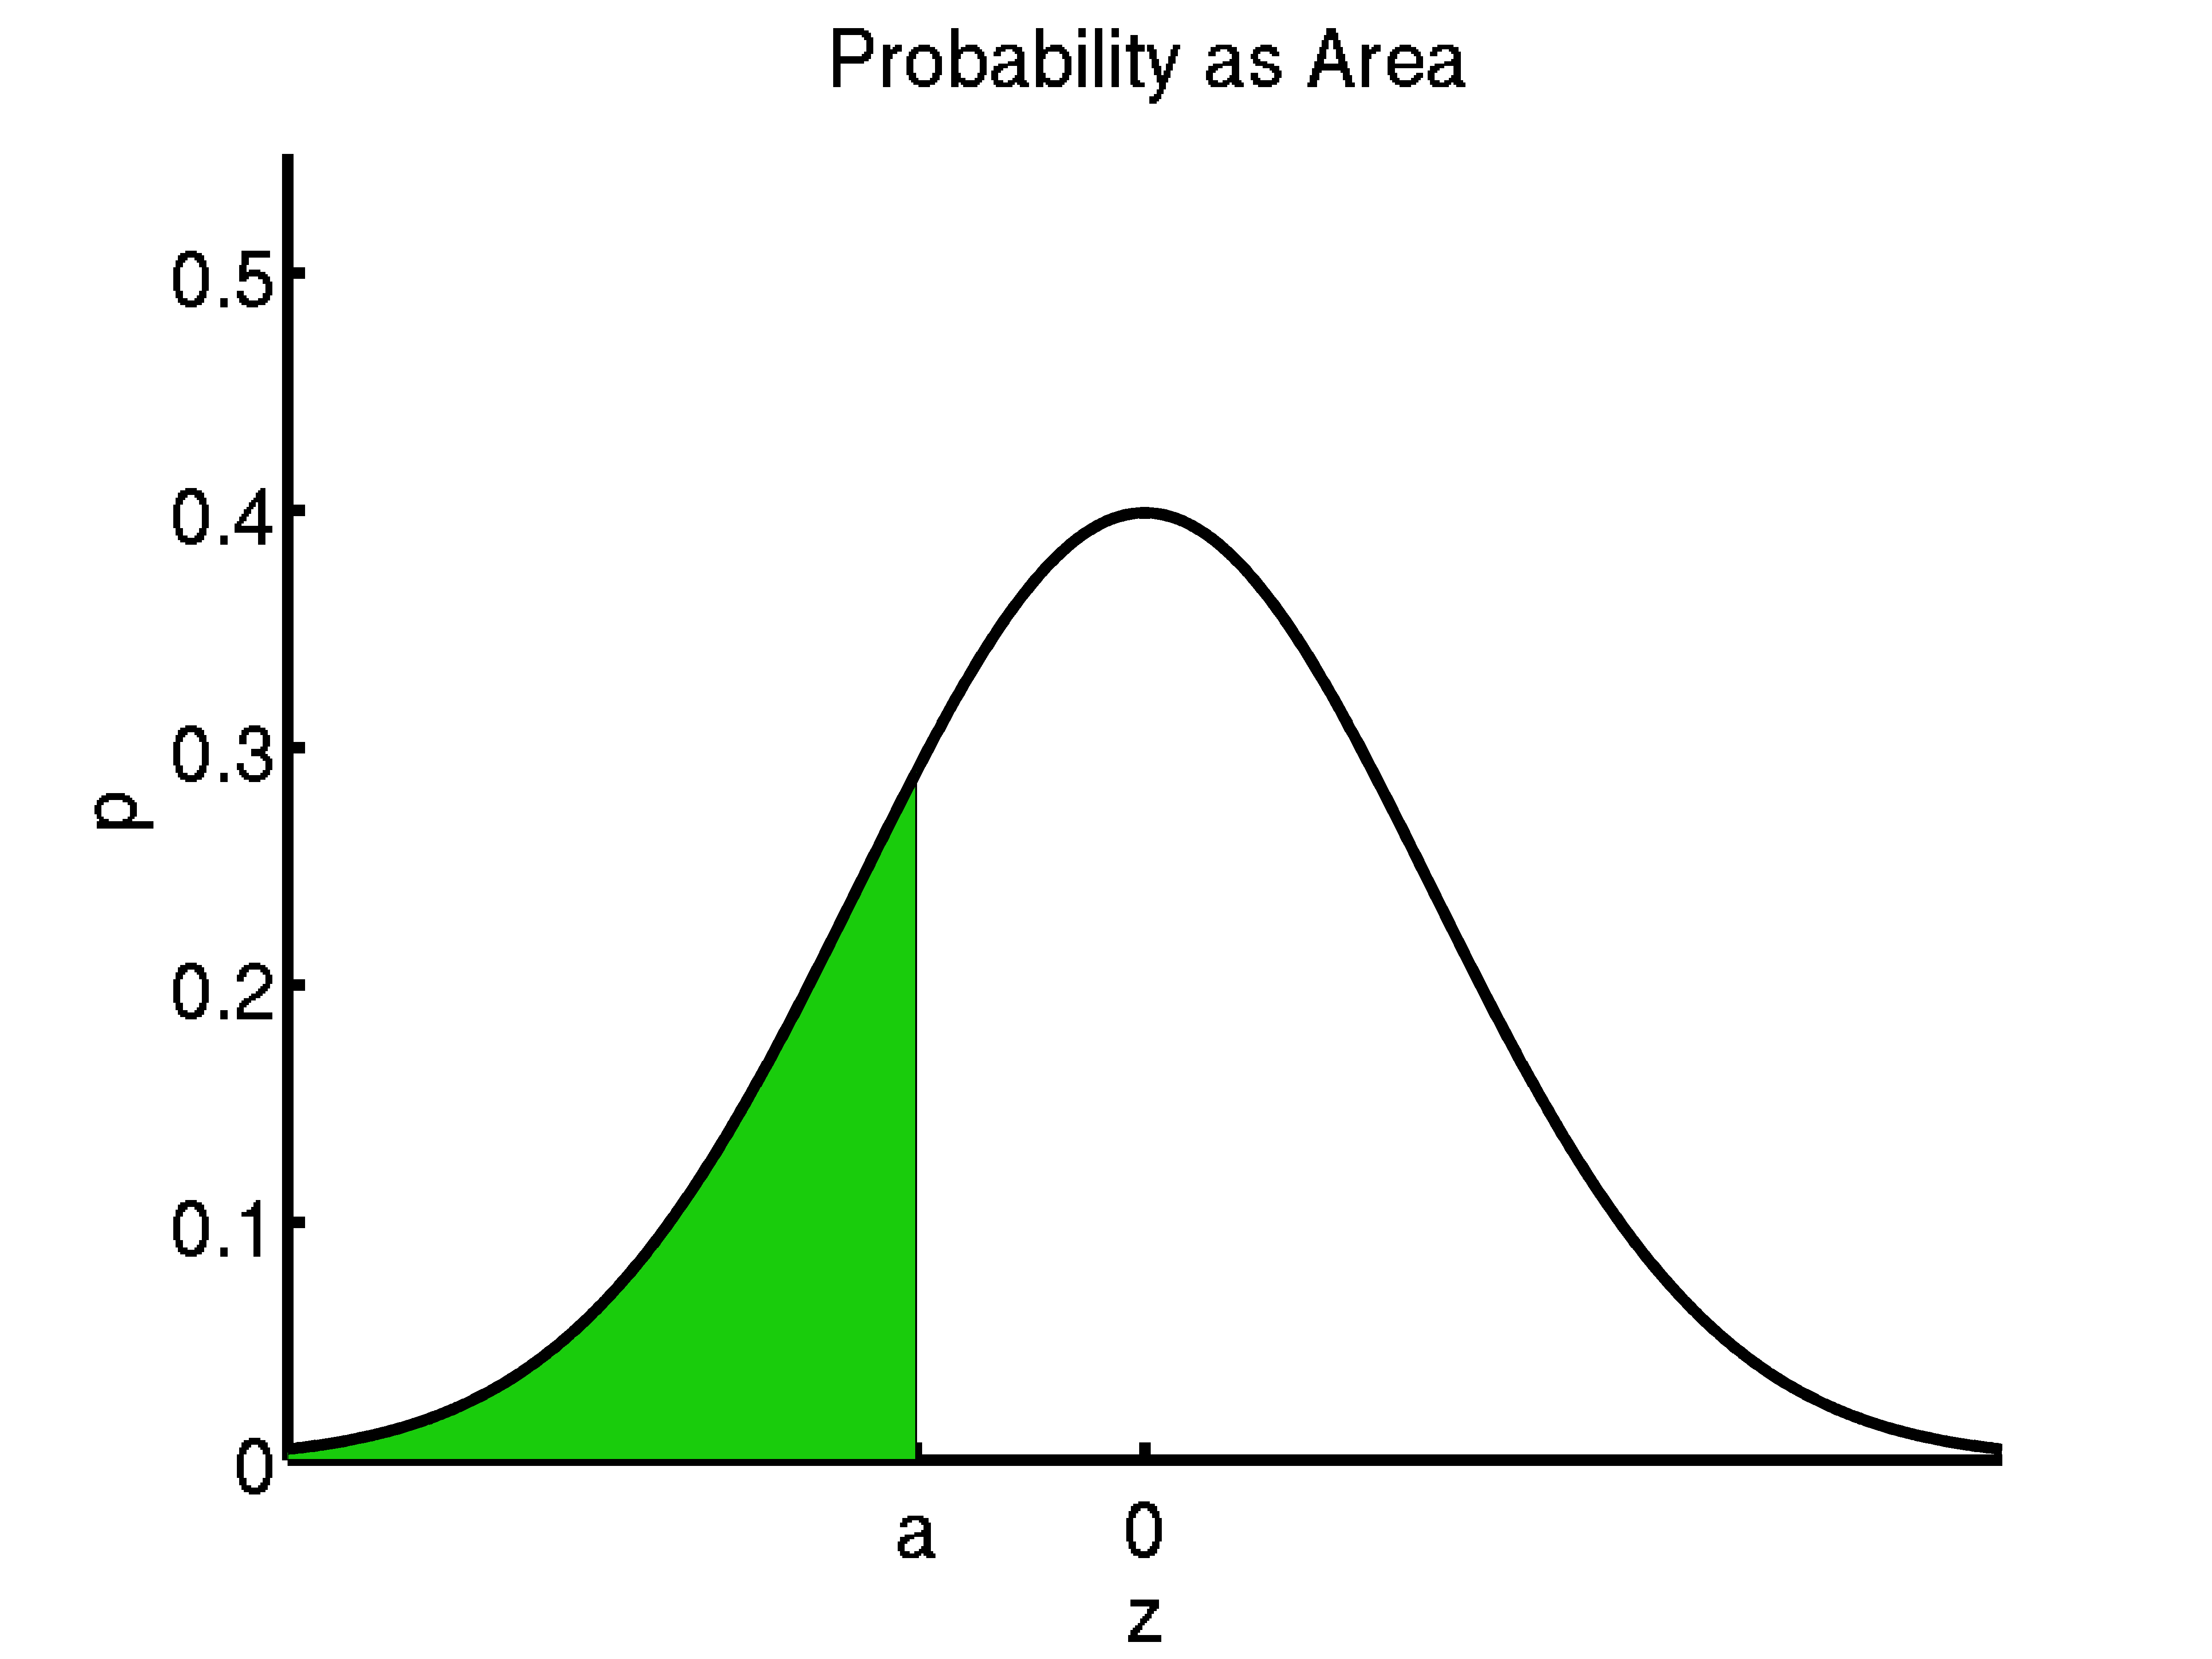
\includegraphics[width=3.55cm]{img/standardNormalArea}
\end{tabular}
  \begin{eqnarray*}
    p(a \leq X \leq b) & = & p(X \leq b) - p(X \leq a)
  \end{eqnarray*}
  
\end{frame}


\subsection{Calculating Probabilities}

\begin{frame}{Calculating the Probability For the Standard Normal}

  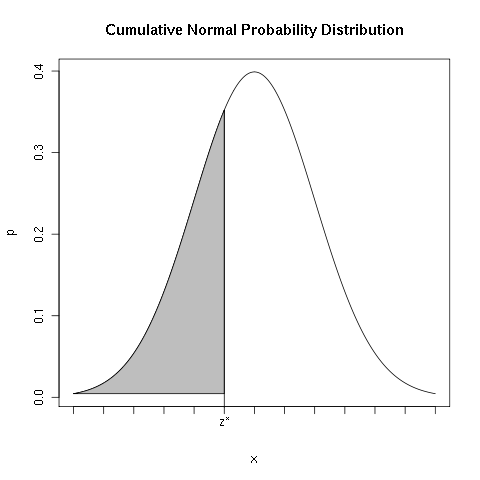
\includegraphics[width=6cm]{img/cummulativeDist}
  
\end{frame}

\begin{frame}
  \frametitle{The Table}
  \vspace*{-5em}
  \hfill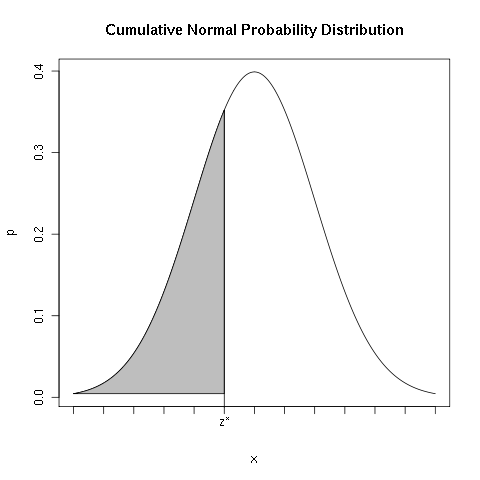
\includegraphics[width=2cm]{img/cummulativeDist}~~~~~~~~~~~~~~

  {
\fontencoding{T1}
\fontfamily{pcr}
\fontseries{m}
\fontshape{n}
\fontsize{5pt}{5pt}
\selectfont

  \begin{tabular}{l|llllllllll}
     & 0.00   & 0.01   & 0.02   & 0.03   &  0.04   & 0.05   & 0.06   & 0.07   & 0.08  & 0.09 \\ \hline
-3.4 & 0.0003 & 0.0003 & 0.0003 & 0.0003 & 0.0003 & 0.0003 & 0.0003 & 0.0003 & 0.0003 & 0.0002 \\ 
-3.3 & 0.0005 & 0.0005 & 0.0005 & 0.0004 & 0.0004 & 0.0004 & 0.0004 & 0.0004 & 0.0004 & 0.0003 \\ 
-3.2 & 0.0007 & 0.0007 & 0.0006 & 0.0006 & 0.0006 & 0.0006 & 0.0006 & 0.0005 & 0.0005 & 0.0005 \\ 
-3.1 & 0.0010 & 0.0009 & 0.0009 & 0.0009 & 0.0008 & 0.0008 & 0.0008 & 0.0008 & 0.0007 & 0.0007 \\ 
-3.0 & 0.0013 & 0.0013 & 0.0013 & 0.0012 & 0.0012 & 0.0011 & 0.0011 & 0.0011 & 0.0010 & 0.0010 \\ 
-2.9 & 0.0019 & 0.0018 & 0.0018 & 0.0017 & 0.0016 & 0.0016 & 0.0015 & 0.0015 & 0.0014 & 0.0014 \\ 
-2.8 & 0.0026 & 0.0025 & 0.0024 & 0.0023 & 0.0023 & 0.0022 & 0.0021 & 0.0021 & 0.0020 & 0.0019 \\ 
-2.7 & 0.0035 & 0.0034 & 0.0033 & 0.0032 & 0.0031 & 0.0030 & 0.0029 & 0.0028 & 0.0027 & 0.0026 \\ 
-2.6 & 0.0047 & 0.0045 & 0.0044 & 0.0043 & 0.0041 & 0.0040 & 0.0039 & 0.0038 & 0.0037 & 0.0036 \\ 
-2.5 & 0.0062 & 0.0060 & 0.0059 & 0.0057 & 0.0055 & 0.0054 & 0.0052 & 0.0051 & 0.0049 & 0.0048 \\ 
-2.4 & 0.0082 & 0.0080 & 0.0078 & 0.0075 & 0.0073 & 0.0071 & 0.0069 & 0.0068 & 0.0066 & 0.0064 \\ 
-2.3 & 0.0107 & 0.0104 & 0.0102 & 0.0099 & 0.0096 & 0.0094 & 0.0091 & 0.0089 & 0.0087 & 0.0084 \\ 
-2.2 & 0.0139 & 0.0136 & 0.0132 & 0.0129 & 0.0125 & 0.0122 & 0.0119 & 0.0116 & 0.0113 & 0.0110 \\ 
-2.1 & 0.0179 & 0.0174 & 0.0170 & 0.0166 & 0.0162 & 0.0158 & 0.0154 & 0.0150 & 0.0146 & 0.0143 \\ 
-2.0 & 0.0228 & 0.0222 & 0.0217 & 0.0212 & 0.0207 & 0.0202 & 0.0197 & 0.0192 & 0.0188 & 0.0183 \\ 
-1.9 & 0.0287 & 0.0281 & 0.0274 & 0.0268 & 0.0262 & 0.0256 & 0.0250 & 0.0244 & 0.0239 & 0.0233 \\ 
-1.8 & 0.0359 & 0.0351 & 0.0344 & 0.0336 & 0.0329 & 0.0322 & 0.0314 & 0.0307 & 0.0301 & 0.0294 \\ 
-1.7 & 0.0446 & 0.0436 & 0.0427 & 0.0418 & 0.0409 & 0.0401 & 0.0392 & 0.0384 & 0.0375 & 0.0367 \\ 
-1.6 & 0.0548 & 0.0537 & 0.0526 & 0.0516 & 0.0505 & 0.0495 & 0.0485 & 0.0475 & 0.0465 & 0.0455 \\ 
-1.5 & 0.0668 & 0.0655 & 0.0643 & 0.0630 & 0.0618 & 0.0606 & 0.0594 & 0.0582 & 0.0571 & 0.0559 \\ 
-1.4 & 0.0808 & 0.0793 & 0.0778 & 0.0764 & 0.0749 & 0.0735 & 0.0721 & 0.0708 & 0.0694 & 0.0681 \\ 
-1.3 & 0.0968 & 0.0951 & 0.0934 & 0.0918 & 0.0901 & 0.0885 & 0.0869 & 0.0853 & 0.0838 & 0.0823 \\ 
-1.2 & 0.1151 & 0.1131 & 0.1112 & 0.1093 & 0.1075 & 0.1056 & 0.1038 & 0.1020 & 0.1003 & 0.0985 \\ 
-1.1 & 0.1357 & 0.1335 & 0.1314 & 0.1292 & 0.1271 & 0.1251 & 0.1230 & 0.1210 & 0.1190 & 0.1170 \\ 
-1.0 & 0.1587 & 0.1562 & 0.1539 & 0.1515 & 0.1492 & 0.1469 & 0.1446 & 0.1423 & 0.1401 & 0.1379 \\ 
-0.9 & 0.1841 & 0.1814 & 0.1788 & 0.1762 & 0.1736 & 0.1711 & 0.1685 & 0.1660 & 0.1635 & 0.1611 \\ 
-0.8 & 0.2119 & 0.2090 & 0.2061 & 0.2033 & 0.2005 & 0.1977 & 0.1949 & 0.1922 & 0.1894 & 0.1867 \\ 
-0.7 & 0.2420 & 0.2389 & 0.2358 & 0.2327 & 0.2296 & 0.2266 & 0.2236 & 0.2206 & 0.2177 & 0.2148 \\ 
-0.6 & 0.2743 & 0.2709 & 0.2676 & 0.2643 & 0.2611 & 0.2578 & 0.2546 & 0.2514 & 0.2483 & 0.2451 \\ 
-0.5 & 0.3085 & 0.3050 & 0.3015 & 0.2981 & 0.2946 & 0.2912 & 0.2877 & 0.2843 & 0.2810 & 0.2776 \\ 
-0.4 & 0.3446 & 0.3409 & 0.3372 & 0.3336 & 0.3300 & 0.3264 & 0.3228 & 0.3192 & 0.3156 & 0.3121 \\ 
-0.3 & 0.3821 & 0.3783 & 0.3745 & 0.3707 & 0.3669 & 0.3632 & 0.3594 & 0.3557 & 0.3520 & 0.3483 \\ 
-0.2 & 0.4207 & 0.4168 & 0.4129 & 0.4090 & 0.4052 & 0.4013 & 0.3974 & 0.3936 & 0.3897 & 0.3859 \\ 
-0.1 & 0.4602 & 0.4562 & 0.4522 & 0.4483 & 0.4443 & 0.4404 & 0.4364 & 0.4325 & 0.4286 & 0.4247 \\ 
-0.0 & 0.5000 & 0.4960 & 0.4920 & 0.4880 & 0.4840 & 0.4801 & 0.4761 & 0.4721 & 0.4681 & 0.4641 
\end{tabular}
}
\end{frame}

\begin{frame}
  \vspace*{-5em}
  \frametitle{The Table}
  \hfill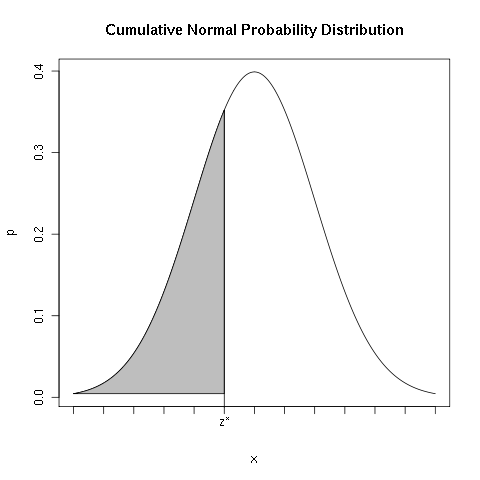
\includegraphics[width=2cm]{img/cummulativeDist}~~~~~~~~~~~~~~

  {
\fontencoding{T1}
\fontfamily{pcr}
\fontseries{m}
\fontshape{n}
\fontsize{5pt}{5pt}
\selectfont
\begin{tabular}{l|llllllllll}
     & 0.00   & 0.01   & 0.02   & 0.03   & 0.04   & 0.05   & 0.06   & 0.07   & 0.08  & 0.09 \\ \hline
0.0 & 0.5000 & 0.5040 & 0.5080 & 0.5120 & 0.5160 & 0.5199 & 0.5239 & 0.5279 & 0.5319 & 0.5359 \\ 
0.1 & 0.5398 & 0.5438 & 0.5478 & 0.5517 & 0.5557 & 0.5596 & 0.5636 & 0.5675 & 0.5714 & 0.5753 \\ 
0.2 & 0.5793 & 0.5832 & 0.5871 & 0.5910 & 0.5948 & 0.5987 & 0.6026 & 0.6064 & 0.6103 & 0.6141 \\ 
0.3 & 0.6179 & 0.6217 & 0.6255 & 0.6293 & 0.6331 & 0.6368 & 0.6406 & 0.6443 & 0.6480 & 0.6517 \\ 
0.4 & 0.6554 & 0.6591 & 0.6628 & 0.6664 & 0.6700 & 0.6736 & 0.6772 & 0.6808 & 0.6844 & 0.6879 \\ 
0.5 & 0.6915 & 0.6950 & 0.6985 & 0.7019 & 0.7054 & 0.7088 & 0.7123 & 0.7157 & 0.7190 & 0.7224 \\ 
0.6 & 0.7257 & 0.7291 & 0.7324 & 0.7357 & 0.7389 & 0.7422 & 0.7454 & 0.7486 & 0.7517 & 0.7549 \\ 
0.7 & 0.7580 & 0.7611 & 0.7642 & 0.7673 & 0.7704 & 0.7734 & 0.7764 & 0.7794 & 0.7823 & 0.7852 \\ 
0.8 & 0.7881 & 0.7910 & 0.7939 & 0.7967 & 0.7995 & 0.8023 & 0.8051 & 0.8078 & 0.8106 & 0.8133 \\ 
0.9 & 0.8159 & 0.8186 & 0.8212 & 0.8238 & 0.8264 & 0.8289 & 0.8315 & 0.8340 & 0.8365 & 0.8389 \\ 
1.0 & 0.8413 & 0.8438 & 0.8461 & 0.8485 & 0.8508 & 0.8531 & 0.8554 & 0.8577 & 0.8599 & 0.8621 \\ 
1.1 & 0.8643 & 0.8665 & 0.8686 & 0.8708 & 0.8729 & 0.8749 & 0.8770 & 0.8790 & 0.8810 & 0.8830 \\ 
1.2 & 0.8849 & 0.8869 & 0.8888 & 0.8907 & 0.8925 & 0.8944 & 0.8962 & 0.8980 & 0.8997 & 0.9015 \\ 
1.3 & 0.9032 & 0.9049 & 0.9066 & 0.9082 & 0.9099 & 0.9115 & 0.9131 & 0.9147 & 0.9162 & 0.9177 \\ 
1.4 & 0.9192 & 0.9207 & 0.9222 & 0.9236 & 0.9251 & 0.9265 & 0.9279 & 0.9292 & 0.9306 & 0.9319 \\ 
1.5 & 0.9332 & 0.9345 & 0.9357 & 0.9370 & 0.9382 & 0.9394 & 0.9406 & 0.9418 & 0.9429 & 0.9441 \\ 
1.6 & 0.9452 & 0.9463 & 0.9474 & 0.9484 & 0.9495 & 0.9505 & 0.9515 & 0.9525 & 0.9535 & 0.9545 \\ 
1.7 & 0.9554 & 0.9564 & 0.9573 & 0.9582 & 0.9591 & 0.9599 & 0.9608 & 0.9616 & 0.9625 & 0.9633 \\ 
1.8 & 0.9641 & 0.9649 & 0.9656 & 0.9664 & 0.9671 & 0.9678 & 0.9686 & 0.9693 & 0.9699 & 0.9706 \\ 
1.9 & 0.9713 & 0.9719 & 0.9726 & 0.9732 & 0.9738 & 0.9744 & 0.9750 & 0.9756 & 0.9761 & 0.9767 \\ 
2.0 & 0.9772 & 0.9778 & 0.9783 & 0.9788 & 0.9793 & 0.9798 & 0.9803 & 0.9808 & 0.9812 & 0.9817 \\ 
2.1 & 0.9821 & 0.9826 & 0.9830 & 0.9834 & 0.9838 & 0.9842 & 0.9846 & 0.9850 & 0.9854 & 0.9857 \\ 
2.2 & 0.9861 & 0.9864 & 0.9868 & 0.9871 & 0.9875 & 0.9878 & 0.9881 & 0.9884 & 0.9887 & 0.9890 \\ 
2.3 & 0.9893 & 0.9896 & 0.9898 & 0.9901 & 0.9904 & 0.9906 & 0.9909 & 0.9911 & 0.9913 & 0.9916 \\ 
2.4 & 0.9918 & 0.9920 & 0.9922 & 0.9925 & 0.9927 & 0.9929 & 0.9931 & 0.9932 & 0.9934 & 0.9936 \\ 
2.5 & 0.9938 & 0.9940 & 0.9941 & 0.9943 & 0.9945 & 0.9946 & 0.9948 & 0.9949 & 0.9951 & 0.9952 \\ 
2.6 & 0.9953 & 0.9955 & 0.9956 & 0.9957 & 0.9959 & 0.9960 & 0.9961 & 0.9962 & 0.9963 & 0.9964 \\ 
2.7 & 0.9965 & 0.9966 & 0.9967 & 0.9968 & 0.9969 & 0.9970 & 0.9971 & 0.9972 & 0.9973 & 0.9974 \\ 
2.8 & 0.9974 & 0.9975 & 0.9976 & 0.9977 & 0.9977 & 0.9978 & 0.9979 & 0.9979 & 0.9980 & 0.9981 \\ 
2.9 & 0.9981 & 0.9982 & 0.9982 & 0.9983 & 0.9984 & 0.9984 & 0.9985 & 0.9985 & 0.9986 & 0.9986 \\ 
3.0 & 0.9987 & 0.9987 & 0.9987 & 0.9988 & 0.9988 & 0.9989 & 0.9989 & 0.9989 & 0.9990 & 0.9990 \\ 
3.1 & 0.9990 & 0.9991 & 0.9991 & 0.9991 & 0.9992 & 0.9992 & 0.9992 & 0.9992 & 0.9993 & 0.9993 \\ 
3.2 & 0.9993 & 0.9993 & 0.9994 & 0.9994 & 0.9994 & 0.9994 & 0.9994 & 0.9995 & 0.9995 & 0.9995 \\ 
3.3 & 0.9995 & 0.9995 & 0.9995 & 0.9996 & 0.9996 & 0.9996 & 0.9996 & 0.9996 & 0.9996 & 0.9997 \\ 
3.4 & 0.9997 & 0.9997 & 0.9997 & 0.9997 & 0.9997 & 0.9997 & 0.9997 & 0.9997 & 0.9997 & 0.9998 
\end{tabular}

}

\end{frame}

\subsection{Examples}

\begin{frame}{\small Find the probability that a standard normal is less than -1.75.}
  
{\small First find the row corresponding to -1.7.}

  {
\fontencoding{T1}
\fontfamily{pcr}
\fontseries{m}
\fontshape{n}
\fontsize{5pt}{5pt}
\selectfont

\begin{tabular}{l|llllllllll}
     & 0.00   & 0.01   & 0.02   & 0.03   &  0.04   & 0.05   & 0.06   & 0.07   & 0.08  & 0.09 \\ \hline
-3.4 & 0.0003 & 0.0003 & 0.0003 & 0.0003 & 0.0003 & 0.0003 & 0.0003 & 0.0003 & 0.0003 & 0.0002 \\ 
-3.3 & 0.0005 & 0.0005 & 0.0005 & 0.0004 & 0.0004 & 0.0004 & 0.0004 & 0.0004 & 0.0004 & 0.0003 \\ 
-3.2 & 0.0007 & 0.0007 & 0.0006 & 0.0006 & 0.0006 & 0.0006 & 0.0006 & 0.0005 & 0.0005 & 0.0005 \\ 
-3.1 & 0.0010 & 0.0009 & 0.0009 & 0.0009 & 0.0008 & 0.0008 & 0.0008 & 0.0008 & 0.0007 & 0.0007 \\ 
-3.0 & 0.0013 & 0.0013 & 0.0013 & 0.0012 & 0.0012 & 0.0011 & 0.0011 & 0.0011 & 0.0010 & 0.0010 \\ 
-2.9 & 0.0019 & 0.0018 & 0.0018 & 0.0017 & 0.0016 & 0.0016 & 0.0015 & 0.0015 & 0.0014 & 0.0014 \\ 
-2.8 & 0.0026 & 0.0025 & 0.0024 & 0.0023 & 0.0023 & 0.0022 & 0.0021 & 0.0021 & 0.0020 & 0.0019 \\ 
-2.7 & 0.0035 & 0.0034 & 0.0033 & 0.0032 & 0.0031 & 0.0030 & 0.0029 & 0.0028 & 0.0027 & 0.0026 \\ 
-2.6 & 0.0047 & 0.0045 & 0.0044 & 0.0043 & 0.0041 & 0.0040 & 0.0039 & 0.0038 & 0.0037 & 0.0036 \\ 
-2.5 & 0.0062 & 0.0060 & 0.0059 & 0.0057 & 0.0055 & 0.0054 & 0.0052 & 0.0051 & 0.0049 & 0.0048 \\ 
-2.4 & 0.0082 & 0.0080 & 0.0078 & 0.0075 & 0.0073 & 0.0071 & 0.0069 & 0.0068 & 0.0066 & 0.0064 \\ 
-2.3 & 0.0107 & 0.0104 & 0.0102 & 0.0099 & 0.0096 & 0.0094 & 0.0091 & 0.0089 & 0.0087 & 0.0084 \\ 
-2.2 & 0.0139 & 0.0136 & 0.0132 & 0.0129 & 0.0125 & 0.0122 & 0.0119 & 0.0116 & 0.0113 & 0.0110 \\ 
-2.1 & 0.0179 & 0.0174 & 0.0170 & 0.0166 & 0.0162 & 0.0158 & 0.0154 & 0.0150 & 0.0146 & 0.0143 \\ 
-2.0 & 0.0228 & 0.0222 & 0.0217 & 0.0212 & 0.0207 & 0.0202 & 0.0197 & 0.0192 & 0.0188 & 0.0183 \\ 
-1.9 & 0.0287 & 0.0281 & 0.0274 & 0.0268 & 0.0262 & 0.0256 & 0.0250 & 0.0244 & 0.0239 & 0.0233 \\ 
-1.8 & 0.0359 & 0.0351 & 0.0344 & 0.0336 & 0.0329 & 0.0322 & 0.0314 & 0.0307 & 0.0301 & 0.0294 \\ 
\rowcolor{red} -1.7 & 0.0446 & 0.0436 & 0.0427 & 0.0418 & 0.0409 & 0.0401 & 0.0392 & 0.0384 & 0.0375 & 0.0367 \\ 
-1.6 & 0.0548 & 0.0537 & 0.0526 & 0.0516 & 0.0505 & 0.0495 & 0.0485 & 0.0475 & 0.0465 & 0.0455 \\ 
-1.5 & 0.0668 & 0.0655 & 0.0643 & 0.0630 & 0.0618 & 0.0606 & 0.0594 & 0.0582 & 0.0571 & 0.0559 \\ 
-1.4 & 0.0808 & 0.0793 & 0.0778 & 0.0764 & 0.0749 & 0.0735 & 0.0721 & 0.0708 & 0.0694 & 0.0681 \\ 
-1.3 & 0.0968 & 0.0951 & 0.0934 & 0.0918 & 0.0901 & 0.0885 & 0.0869 & 0.0853 & 0.0838 & 0.0823 \\ 
-1.2 & 0.1151 & 0.1131 & 0.1112 & 0.1093 & 0.1075 & 0.1056 & 0.1038 & 0.1020 & 0.1003 & 0.0985 \\ 
-1.1 & 0.1357 & 0.1335 & 0.1314 & 0.1292 & 0.1271 & 0.1251 & 0.1230 & 0.1210 & 0.1190 & 0.1170 \\ 
-1.0 & 0.1587 & 0.1562 & 0.1539 & 0.1515 & 0.1492 & 0.1469 & 0.1446 & 0.1423 & 0.1401 & 0.1379 \\ 
-0.9 & 0.1841 & 0.1814 & 0.1788 & 0.1762 & 0.1736 & 0.1711 & 0.1685 & 0.1660 & 0.1635 & 0.1611 \\ 
-0.8 & 0.2119 & 0.2090 & 0.2061 & 0.2033 & 0.2005 & 0.1977 & 0.1949 & 0.1922 & 0.1894 & 0.1867 \\ 
-0.7 & 0.2420 & 0.2389 & 0.2358 & 0.2327 & 0.2296 & 0.2266 & 0.2236 & 0.2206 & 0.2177 & 0.2148 \\ 
-0.6 & 0.2743 & 0.2709 & 0.2676 & 0.2643 & 0.2611 & 0.2578 & 0.2546 & 0.2514 & 0.2483 & 0.2451 \\ 
-0.5 & 0.3085 & 0.3050 & 0.3015 & 0.2981 & 0.2946 & 0.2912 & 0.2877 & 0.2843 & 0.2810 & 0.2776 \\ 
-0.4 & 0.3446 & 0.3409 & 0.3372 & 0.3336 & 0.3300 & 0.3264 & 0.3228 & 0.3192 & 0.3156 & 0.3121 \\ 
-0.3 & 0.3821 & 0.3783 & 0.3745 & 0.3707 & 0.3669 & 0.3632 & 0.3594 & 0.3557 & 0.3520 & 0.3483 \\ 
-0.2 & 0.4207 & 0.4168 & 0.4129 & 0.4090 & 0.4052 & 0.4013 & 0.3974 & 0.3936 & 0.3897 & 0.3859 \\ 
-0.1 & 0.4602 & 0.4562 & 0.4522 & 0.4483 & 0.4443 & 0.4404 & 0.4364 & 0.4325 & 0.4286 & 0.4247 \\ 
-0.0 & 0.5000 & 0.4960 & 0.4920 & 0.4880 & 0.4840 & 0.4801 & 0.4761 & 0.4721 & 0.4681 & 0.4641 
\end{tabular}


}


\end{frame}

\begin{frame} {\small First find the row corresponding to -1.7. Second
    find the column corresponding to 0.05. The probability is the
    intersection of the row and column, 0.0401.}

  {
\fontencoding{T1}
\fontfamily{pcr}
\fontseries{m}
\fontshape{n}
\fontsize{5pt}{5pt}
\selectfont

\begin{tabular}{l|lllll>{\columncolor{blue}}lllll}
     & 0.00   & 0.01   & 0.02   & 0.03   &  0.04   & 0.05   & 0.06   & 0.07   & 0.08  & 0.09 \\ \hline
-3.4 & 0.0003 & 0.0003 & 0.0003 & 0.0003 & 0.0003 & 0.0003 & 0.0003 & 0.0003 & 0.0003 & 0.0002 \\ 
-3.3 & 0.0005 & 0.0005 & 0.0005 & 0.0004 & 0.0004 & 0.0004 & 0.0004 & 0.0004 & 0.0004 & 0.0003 \\ 
-3.2 & 0.0007 & 0.0007 & 0.0006 & 0.0006 & 0.0006 & 0.0006 & 0.0006 & 0.0005 & 0.0005 & 0.0005 \\ 
-3.1 & 0.0010 & 0.0009 & 0.0009 & 0.0009 & 0.0008 & 0.0008 & 0.0008 & 0.0008 & 0.0007 & 0.0007 \\ 
-3.0 & 0.0013 & 0.0013 & 0.0013 & 0.0012 & 0.0012 & 0.0011 & 0.0011 & 0.0011 & 0.0010 & 0.0010 \\ 
-2.9 & 0.0019 & 0.0018 & 0.0018 & 0.0017 & 0.0016 & 0.0016 & 0.0015 & 0.0015 & 0.0014 & 0.0014 \\ 
-2.8 & 0.0026 & 0.0025 & 0.0024 & 0.0023 & 0.0023 & 0.0022 & 0.0021 & 0.0021 & 0.0020 & 0.0019 \\ 
-2.7 & 0.0035 & 0.0034 & 0.0033 & 0.0032 & 0.0031 & 0.0030 & 0.0029 & 0.0028 & 0.0027 & 0.0026 \\ 
-2.6 & 0.0047 & 0.0045 & 0.0044 & 0.0043 & 0.0041 & 0.0040 & 0.0039 & 0.0038 & 0.0037 & 0.0036 \\ 
-2.5 & 0.0062 & 0.0060 & 0.0059 & 0.0057 & 0.0055 & 0.0054 & 0.0052 & 0.0051 & 0.0049 & 0.0048 \\ 
-2.4 & 0.0082 & 0.0080 & 0.0078 & 0.0075 & 0.0073 & 0.0071 & 0.0069 & 0.0068 & 0.0066 & 0.0064 \\ 
-2.3 & 0.0107 & 0.0104 & 0.0102 & 0.0099 & 0.0096 & 0.0094 & 0.0091 & 0.0089 & 0.0087 & 0.0084 \\ 
-2.2 & 0.0139 & 0.0136 & 0.0132 & 0.0129 & 0.0125 & 0.0122 & 0.0119 & 0.0116 & 0.0113 & 0.0110 \\ 
-2.1 & 0.0179 & 0.0174 & 0.0170 & 0.0166 & 0.0162 & 0.0158 & 0.0154 & 0.0150 & 0.0146 & 0.0143 \\ 
-2.0 & 0.0228 & 0.0222 & 0.0217 & 0.0212 & 0.0207 & 0.0202 & 0.0197 & 0.0192 & 0.0188 & 0.0183 \\ 
-1.9 & 0.0287 & 0.0281 & 0.0274 & 0.0268 & 0.0262 & 0.0256 & 0.0250 & 0.0244 & 0.0239 & 0.0233 \\ 
-1.8 & 0.0359 & 0.0351 & 0.0344 & 0.0336 & 0.0329 & 0.0322 & 0.0314 & 0.0307 & 0.0301 & 0.0294 \\ 
\rowcolor{red} -1.7 & 0.0446 & 0.0436 & 0.0427 & 0.0418 & 0.0409 & {\colorbox{yellow}{~~0.0401}~~} & 0.0392 & 0.0384 & 0.0375 & 0.0367 \\ 
-1.6 & 0.0548 & 0.0537 & 0.0526 & 0.0516 & 0.0505 & 0.0495 & 0.0485 & 0.0475 & 0.0465 & 0.0455 \\ 
-1.5 & 0.0668 & 0.0655 & 0.0643 & 0.0630 & 0.0618 & 0.0606 & 0.0594 & 0.0582 & 0.0571 & 0.0559 \\ 
-1.4 & 0.0808 & 0.0793 & 0.0778 & 0.0764 & 0.0749 & 0.0735 & 0.0721 & 0.0708 & 0.0694 & 0.0681 \\ 
-1.3 & 0.0968 & 0.0951 & 0.0934 & 0.0918 & 0.0901 & 0.0885 & 0.0869 & 0.0853 & 0.0838 & 0.0823 \\ 
-1.2 & 0.1151 & 0.1131 & 0.1112 & 0.1093 & 0.1075 & 0.1056 & 0.1038 & 0.1020 & 0.1003 & 0.0985 \\ 
-1.1 & 0.1357 & 0.1335 & 0.1314 & 0.1292 & 0.1271 & 0.1251 & 0.1230 & 0.1210 & 0.1190 & 0.1170 \\ 
-1.0 & 0.1587 & 0.1562 & 0.1539 & 0.1515 & 0.1492 & 0.1469 & 0.1446 & 0.1423 & 0.1401 & 0.1379 \\ 
-0.9 & 0.1841 & 0.1814 & 0.1788 & 0.1762 & 0.1736 & 0.1711 & 0.1685 & 0.1660 & 0.1635 & 0.1611 \\ 
-0.8 & 0.2119 & 0.2090 & 0.2061 & 0.2033 & 0.2005 & 0.1977 & 0.1949 & 0.1922 & 0.1894 & 0.1867 \\ 
-0.7 & 0.2420 & 0.2389 & 0.2358 & 0.2327 & 0.2296 & 0.2266 & 0.2236 & 0.2206 & 0.2177 & 0.2148 \\ 
-0.6 & 0.2743 & 0.2709 & 0.2676 & 0.2643 & 0.2611 & 0.2578 & 0.2546 & 0.2514 & 0.2483 & 0.2451 \\ 
-0.5 & 0.3085 & 0.3050 & 0.3015 & 0.2981 & 0.2946 & 0.2912 & 0.2877 & 0.2843 & 0.2810 & 0.2776 \\ 
-0.4 & 0.3446 & 0.3409 & 0.3372 & 0.3336 & 0.3300 & 0.3264 & 0.3228 & 0.3192 & 0.3156 & 0.3121 \\ 
-0.3 & 0.3821 & 0.3783 & 0.3745 & 0.3707 & 0.3669 & 0.3632 & 0.3594 & 0.3557 & 0.3520 & 0.3483 \\ 
-0.2 & 0.4207 & 0.4168 & 0.4129 & 0.4090 & 0.4052 & 0.4013 & 0.3974 & 0.3936 & 0.3897 & 0.3859 \\ 
-0.1 & 0.4602 & 0.4562 & 0.4522 & 0.4483 & 0.4443 & 0.4404 & 0.4364 & 0.4325 & 0.4286 & 0.4247 \\ 
-0.0 & 0.5000 & 0.4960 & 0.4920 & 0.4880 & 0.4840 & 0.4801 & 0.4761 & 0.4721 & 0.4681 & 0.4641 
\end{tabular}



}

\end{frame}




\begin{frame}{\small Find the probability that a standard normal is less than 0.87.}
  
{\small First find the row corresponding to 0.8.}

  {
\fontencoding{T1}
\fontfamily{pcr}
\fontseries{m}
\fontshape{n}
\fontsize{5pt}{5pt}
\selectfont

\begin{tabular}{l|llllllllll}
     & 0.00   & 0.01   & 0.02   & 0.03   & 0.04   & 0.05   & 0.06   & 0.07   & 0.08  & 0.09 \\ \hline
0.0 & 0.5000 & 0.5040 & 0.5080 & 0.5120 & 0.5160 & 0.5199 & 0.5239 & 0.5279 & 0.5319 & 0.5359 \\ 
0.1 & 0.5398 & 0.5438 & 0.5478 & 0.5517 & 0.5557 & 0.5596 & 0.5636 & 0.5675 & 0.5714 & 0.5753 \\ 
0.2 & 0.5793 & 0.5832 & 0.5871 & 0.5910 & 0.5948 & 0.5987 & 0.6026 & 0.6064 & 0.6103 & 0.6141 \\ 
0.3 & 0.6179 & 0.6217 & 0.6255 & 0.6293 & 0.6331 & 0.6368 & 0.6406 & 0.6443 & 0.6480 & 0.6517 \\ 
0.4 & 0.6554 & 0.6591 & 0.6628 & 0.6664 & 0.6700 & 0.6736 & 0.6772 & 0.6808 & 0.6844 & 0.6879 \\ 
0.5 & 0.6915 & 0.6950 & 0.6985 & 0.7019 & 0.7054 & 0.7088 & 0.7123 & 0.7157 & 0.7190 & 0.7224 \\ 
0.6 & 0.7257 & 0.7291 & 0.7324 & 0.7357 & 0.7389 & 0.7422 & 0.7454 & 0.7486 & 0.7517 & 0.7549 \\ 
0.7 & 0.7580 & 0.7611 & 0.7642 & 0.7673 & 0.7704 & 0.7734 & 0.7764 & 0.7794 & 0.7823 & 0.7852 \\ 
\rowcolor{red}0.8 & 0.7881 & 0.7910 & 0.7939 & 0.7967 & 0.7995 & 0.8023 & 0.8051 & 0.8078 & 0.8106 & 0.8133 \\ 
0.9 & 0.8159 & 0.8186 & 0.8212 & 0.8238 & 0.8264 & 0.8289 & 0.8315 & 0.8340 & 0.8365 & 0.8389 \\ 
1.0 & 0.8413 & 0.8438 & 0.8461 & 0.8485 & 0.8508 & 0.8531 & 0.8554 & 0.8577 & 0.8599 & 0.8621 \\ 
1.1 & 0.8643 & 0.8665 & 0.8686 & 0.8708 & 0.8729 & 0.8749 & 0.8770 & 0.8790 & 0.8810 & 0.8830 \\ 
1.2 & 0.8849 & 0.8869 & 0.8888 & 0.8907 & 0.8925 & 0.8944 & 0.8962 & 0.8980 & 0.8997 & 0.9015 \\ 
1.3 & 0.9032 & 0.9049 & 0.9066 & 0.9082 & 0.9099 & 0.9115 & 0.9131 & 0.9147 & 0.9162 & 0.9177 \\ 
1.4 & 0.9192 & 0.9207 & 0.9222 & 0.9236 & 0.9251 & 0.9265 & 0.9279 & 0.9292 & 0.9306 & 0.9319 \\ 
1.5 & 0.9332 & 0.9345 & 0.9357 & 0.9370 & 0.9382 & 0.9394 & 0.9406 & 0.9418 & 0.9429 & 0.9441 \\ 
1.6 & 0.9452 & 0.9463 & 0.9474 & 0.9484 & 0.9495 & 0.9505 & 0.9515 & 0.9525 & 0.9535 & 0.9545 \\ 
1.7 & 0.9554 & 0.9564 & 0.9573 & 0.9582 & 0.9591 & 0.9599 & 0.9608 & 0.9616 & 0.9625 & 0.9633 \\ 
1.8 & 0.9641 & 0.9649 & 0.9656 & 0.9664 & 0.9671 & 0.9678 & 0.9686 & 0.9693 & 0.9699 & 0.9706 \\ 
1.9 & 0.9713 & 0.9719 & 0.9726 & 0.9732 & 0.9738 & 0.9744 & 0.9750 & 0.9756 & 0.9761 & 0.9767 \\ 
2.0 & 0.9772 & 0.9778 & 0.9783 & 0.9788 & 0.9793 & 0.9798 & 0.9803 & 0.9808 & 0.9812 & 0.9817 \\ 
2.1 & 0.9821 & 0.9826 & 0.9830 & 0.9834 & 0.9838 & 0.9842 & 0.9846 & 0.9850 & 0.9854 & 0.9857 \\ 
2.2 & 0.9861 & 0.9864 & 0.9868 & 0.9871 & 0.9875 & 0.9878 & 0.9881 & 0.9884 & 0.9887 & 0.9890 \\ 
2.3 & 0.9893 & 0.9896 & 0.9898 & 0.9901 & 0.9904 & 0.9906 & 0.9909 & 0.9911 & 0.9913 & 0.9916 \\ 
2.4 & 0.9918 & 0.9920 & 0.9922 & 0.9925 & 0.9927 & 0.9929 & 0.9931 & 0.9932 & 0.9934 & 0.9936 \\ 
2.5 & 0.9938 & 0.9940 & 0.9941 & 0.9943 & 0.9945 & 0.9946 & 0.9948 & 0.9949 & 0.9951 & 0.9952 \\ 
2.6 & 0.9953 & 0.9955 & 0.9956 & 0.9957 & 0.9959 & 0.9960 & 0.9961 & 0.9962 & 0.9963 & 0.9964 \\ 
2.7 & 0.9965 & 0.9966 & 0.9967 & 0.9968 & 0.9969 & 0.9970 & 0.9971 & 0.9972 & 0.9973 & 0.9974 \\ 
2.8 & 0.9974 & 0.9975 & 0.9976 & 0.9977 & 0.9977 & 0.9978 & 0.9979 & 0.9979 & 0.9980 & 0.9981 \\ 
2.9 & 0.9981 & 0.9982 & 0.9982 & 0.9983 & 0.9984 & 0.9984 & 0.9985 & 0.9985 & 0.9986 & 0.9986 \\ 
3.0 & 0.9987 & 0.9987 & 0.9987 & 0.9988 & 0.9988 & 0.9989 & 0.9989 & 0.9989 & 0.9990 & 0.9990 \\ 
3.1 & 0.9990 & 0.9991 & 0.9991 & 0.9991 & 0.9992 & 0.9992 & 0.9992 & 0.9992 & 0.9993 & 0.9993 \\ 
3.2 & 0.9993 & 0.9993 & 0.9994 & 0.9994 & 0.9994 & 0.9994 & 0.9994 & 0.9995 & 0.9995 & 0.9995 \\ 
3.3 & 0.9995 & 0.9995 & 0.9995 & 0.9996 & 0.9996 & 0.9996 & 0.9996 & 0.9996 & 0.9996 & 0.9997 \\ 
3.4 & 0.9997 & 0.9997 & 0.9997 & 0.9997 & 0.9997 & 0.9997 & 0.9997 & 0.9997 & 0.9997 & 0.9998 
\end{tabular}


}


\end{frame}

\begin{frame}
{\small Second find the column corresponding to 0.07. The probability is the
intersection of the row and column, 0.8078.}

  {
\fontencoding{T1}
\fontfamily{pcr}
\fontseries{m}
\fontshape{n}
\fontsize{5pt}{5pt}
\selectfont

\begin{tabular}{l|lllllll>{\columncolor{blue}}lll}
     & 0.00   & 0.01   & 0.02   & 0.03   & 0.04   & 0.05   & 0.06   & 0.07   & 0.08  & 0.09 \\ \hline
0.0 & 0.5000 & 0.5040 & 0.5080 & 0.5120 & 0.5160 & 0.5199 & 0.5239 & 0.5279 & 0.5319 & 0.5359 \\ 
0.1 & 0.5398 & 0.5438 & 0.5478 & 0.5517 & 0.5557 & 0.5596 & 0.5636 & 0.5675 & 0.5714 & 0.5753 \\ 
0.2 & 0.5793 & 0.5832 & 0.5871 & 0.5910 & 0.5948 & 0.5987 & 0.6026 & 0.6064 & 0.6103 & 0.6141 \\ 
0.3 & 0.6179 & 0.6217 & 0.6255 & 0.6293 & 0.6331 & 0.6368 & 0.6406 & 0.6443 & 0.6480 & 0.6517 \\ 
0.4 & 0.6554 & 0.6591 & 0.6628 & 0.6664 & 0.6700 & 0.6736 & 0.6772 & 0.6808 & 0.6844 & 0.6879 \\ 
0.5 & 0.6915 & 0.6950 & 0.6985 & 0.7019 & 0.7054 & 0.7088 & 0.7123 & 0.7157 & 0.7190 & 0.7224 \\ 
0.6 & 0.7257 & 0.7291 & 0.7324 & 0.7357 & 0.7389 & 0.7422 & 0.7454 & 0.7486 & 0.7517 & 0.7549 \\ 
0.7 & 0.7580 & 0.7611 & 0.7642 & 0.7673 & 0.7704 & 0.7734 & 0.7764 & 0.7794 & 0.7823 & 0.7852 \\ 
\rowcolor{red}0.8 & 0.7881 & 0.7910 & 0.7939 & 0.7967 & 0.7995 & 0.8023 & 0.8051 & {\colorbox{yellow}{~~0.8078~~}} & 0.8106 & 0.8133 \\ 
0.9 & 0.8159 & 0.8186 & 0.8212 & 0.8238 & 0.8264 & 0.8289 & 0.8315 & 0.8340 & 0.8365 & 0.8389 \\ 
1.0 & 0.8413 & 0.8438 & 0.8461 & 0.8485 & 0.8508 & 0.8531 & 0.8554 & 0.8577 & 0.8599 & 0.8621 \\ 
1.1 & 0.8643 & 0.8665 & 0.8686 & 0.8708 & 0.8729 & 0.8749 & 0.8770 & 0.8790 & 0.8810 & 0.8830 \\ 
1.2 & 0.8849 & 0.8869 & 0.8888 & 0.8907 & 0.8925 & 0.8944 & 0.8962 & 0.8980 & 0.8997 & 0.9015 \\ 
1.3 & 0.9032 & 0.9049 & 0.9066 & 0.9082 & 0.9099 & 0.9115 & 0.9131 & 0.9147 & 0.9162 & 0.9177 \\ 
1.4 & 0.9192 & 0.9207 & 0.9222 & 0.9236 & 0.9251 & 0.9265 & 0.9279 & 0.9292 & 0.9306 & 0.9319 \\ 
1.5 & 0.9332 & 0.9345 & 0.9357 & 0.9370 & 0.9382 & 0.9394 & 0.9406 & 0.9418 & 0.9429 & 0.9441 \\ 
1.6 & 0.9452 & 0.9463 & 0.9474 & 0.9484 & 0.9495 & 0.9505 & 0.9515 & 0.9525 & 0.9535 & 0.9545 \\ 
1.7 & 0.9554 & 0.9564 & 0.9573 & 0.9582 & 0.9591 & 0.9599 & 0.9608 & 0.9616 & 0.9625 & 0.9633 \\ 
1.8 & 0.9641 & 0.9649 & 0.9656 & 0.9664 & 0.9671 & 0.9678 & 0.9686 & 0.9693 & 0.9699 & 0.9706 \\ 
1.9 & 0.9713 & 0.9719 & 0.9726 & 0.9732 & 0.9738 & 0.9744 & 0.9750 & 0.9756 & 0.9761 & 0.9767 \\ 
2.0 & 0.9772 & 0.9778 & 0.9783 & 0.9788 & 0.9793 & 0.9798 & 0.9803 & 0.9808 & 0.9812 & 0.9817 \\ 
2.1 & 0.9821 & 0.9826 & 0.9830 & 0.9834 & 0.9838 & 0.9842 & 0.9846 & 0.9850 & 0.9854 & 0.9857 \\ 
2.2 & 0.9861 & 0.9864 & 0.9868 & 0.9871 & 0.9875 & 0.9878 & 0.9881 & 0.9884 & 0.9887 & 0.9890 \\ 
2.3 & 0.9893 & 0.9896 & 0.9898 & 0.9901 & 0.9904 & 0.9906 & 0.9909 & 0.9911 & 0.9913 & 0.9916 \\ 
2.4 & 0.9918 & 0.9920 & 0.9922 & 0.9925 & 0.9927 & 0.9929 & 0.9931 & 0.9932 & 0.9934 & 0.9936 \\ 
2.5 & 0.9938 & 0.9940 & 0.9941 & 0.9943 & 0.9945 & 0.9946 & 0.9948 & 0.9949 & 0.9951 & 0.9952 \\ 
2.6 & 0.9953 & 0.9955 & 0.9956 & 0.9957 & 0.9959 & 0.9960 & 0.9961 & 0.9962 & 0.9963 & 0.9964 \\ 
2.7 & 0.9965 & 0.9966 & 0.9967 & 0.9968 & 0.9969 & 0.9970 & 0.9971 & 0.9972 & 0.9973 & 0.9974 \\ 
2.8 & 0.9974 & 0.9975 & 0.9976 & 0.9977 & 0.9977 & 0.9978 & 0.9979 & 0.9979 & 0.9980 & 0.9981 \\ 
2.9 & 0.9981 & 0.9982 & 0.9982 & 0.9983 & 0.9984 & 0.9984 & 0.9985 & 0.9985 & 0.9986 & 0.9986 \\ 
3.0 & 0.9987 & 0.9987 & 0.9987 & 0.9988 & 0.9988 & 0.9989 & 0.9989 & 0.9989 & 0.9990 & 0.9990 \\ 
3.1 & 0.9990 & 0.9991 & 0.9991 & 0.9991 & 0.9992 & 0.9992 & 0.9992 & 0.9992 & 0.9993 & 0.9993 \\ 
3.2 & 0.9993 & 0.9993 & 0.9994 & 0.9994 & 0.9994 & 0.9994 & 0.9994 & 0.9995 & 0.9995 & 0.9995 \\ 
3.3 & 0.9995 & 0.9995 & 0.9995 & 0.9996 & 0.9996 & 0.9996 & 0.9996 & 0.9996 & 0.9996 & 0.9997 \\ 
3.4 & 0.9997 & 0.9997 & 0.9997 & 0.9997 & 0.9997 & 0.9997 & 0.9997 & 0.9997 & 0.9997 & 0.9998 
\end{tabular}



}

\end{frame}


\begin{frame}

  Determine $p(-1.32 \leq z \leq 2.56)$.

  \hfill

\end{frame}

\iftoggle{clicker}{%
  \begin{frame}
    \frametitle{Clicker Quiz}

    Find $p(1.46 \leq Z \leq 2.13)$.
    \vfill

    \begin{tabular}{l@{\hspace{3em}}l@{\hspace{3em}}l@{\hspace{3em}}l}
      A: 0.0555 & B: 0.0703  & C: 0.6700 & D: 0.9834
    \end{tabular}
    % .9834-.9279 = 0.0555

    \vfill
    \vfill
    \vfill


  \end{frame}
}


\begin{frame}{Going Backwards}

  If $p(z \leq a) \approx 0.9834$ what is $a$?

  \hfill

  \uncover<2->{If $p(z \geq a) \approx 0.05$ what is $a$?}

   \hfill
  
\end{frame}


% LocalWords:  Clarkson pausesection hideallsubsections


\lecture{Normal Distributions}{normal-distributions-not-standard}
\section{Normal Distributions}

\title{Normal Distributions}
\subtitle{Distributions That Are Not The Standard Normal}

%\author{Kelly Black}
%\institute{Clarkson University}
\date{February 1 2013}

\begin{frame}
  \titlepage
\end{frame}

\begin{frame}
  \frametitle{Outline}
  \tableofcontents[pausesection,hideothersubsections,sectionstyle=show/hide]
\end{frame}


\subsection{Clicker Quiz}

\iftoggle{clicker}{%
  \begin{frame}
    \frametitle{Clicker Quiz}

    What is the probability that a random variable that follows a
    standard normal distribution is less than 1.47?

    \vfill

    \begin{tabular}{l@{\hspace{3em}}l@{\hspace{3em}}l}
      A: .9147 & B: .9292 & C: .9418 
    \end{tabular}

    \vfill
    \vfill
    \vfill


  \end{frame}
}


\begin{frame}
  \frametitle{The Table}
  \vspace*{-5em}
  \hfill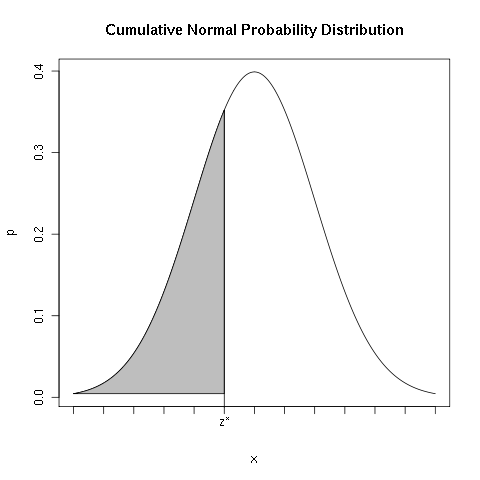
\includegraphics[width=2cm]{img/cummulativeDist}~~~~~~~~~~~~~~

  {
\fontencoding{T1}
\fontfamily{pcr}
\fontseries{m}
\fontshape{n}
\fontsize{5pt}{5pt}
\selectfont

  \begin{tabular}{l|llllllllll}
     & 0.00   & 0.01   & 0.02   & 0.03   &  0.04   & 0.05   & 0.06   & 0.07   & 0.08  & 0.09 \\ \hline
-3.4 & 0.0003 & 0.0003 & 0.0003 & 0.0003 & 0.0003 & 0.0003 & 0.0003 & 0.0003 & 0.0003 & 0.0002 \\ 
-3.3 & 0.0005 & 0.0005 & 0.0005 & 0.0004 & 0.0004 & 0.0004 & 0.0004 & 0.0004 & 0.0004 & 0.0003 \\ 
-3.2 & 0.0007 & 0.0007 & 0.0006 & 0.0006 & 0.0006 & 0.0006 & 0.0006 & 0.0005 & 0.0005 & 0.0005 \\ 
-3.1 & 0.0010 & 0.0009 & 0.0009 & 0.0009 & 0.0008 & 0.0008 & 0.0008 & 0.0008 & 0.0007 & 0.0007 \\ 
-3.0 & 0.0013 & 0.0013 & 0.0013 & 0.0012 & 0.0012 & 0.0011 & 0.0011 & 0.0011 & 0.0010 & 0.0010 \\ 
-2.9 & 0.0019 & 0.0018 & 0.0018 & 0.0017 & 0.0016 & 0.0016 & 0.0015 & 0.0015 & 0.0014 & 0.0014 \\ 
-2.8 & 0.0026 & 0.0025 & 0.0024 & 0.0023 & 0.0023 & 0.0022 & 0.0021 & 0.0021 & 0.0020 & 0.0019 \\ 
-2.7 & 0.0035 & 0.0034 & 0.0033 & 0.0032 & 0.0031 & 0.0030 & 0.0029 & 0.0028 & 0.0027 & 0.0026 \\ 
-2.6 & 0.0047 & 0.0045 & 0.0044 & 0.0043 & 0.0041 & 0.0040 & 0.0039 & 0.0038 & 0.0037 & 0.0036 \\ 
-2.5 & 0.0062 & 0.0060 & 0.0059 & 0.0057 & 0.0055 & 0.0054 & 0.0052 & 0.0051 & 0.0049 & 0.0048 \\ 
-2.4 & 0.0082 & 0.0080 & 0.0078 & 0.0075 & 0.0073 & 0.0071 & 0.0069 & 0.0068 & 0.0066 & 0.0064 \\ 
-2.3 & 0.0107 & 0.0104 & 0.0102 & 0.0099 & 0.0096 & 0.0094 & 0.0091 & 0.0089 & 0.0087 & 0.0084 \\ 
-2.2 & 0.0139 & 0.0136 & 0.0132 & 0.0129 & 0.0125 & 0.0122 & 0.0119 & 0.0116 & 0.0113 & 0.0110 \\ 
-2.1 & 0.0179 & 0.0174 & 0.0170 & 0.0166 & 0.0162 & 0.0158 & 0.0154 & 0.0150 & 0.0146 & 0.0143 \\ 
-2.0 & 0.0228 & 0.0222 & 0.0217 & 0.0212 & 0.0207 & 0.0202 & 0.0197 & 0.0192 & 0.0188 & 0.0183 \\ 
-1.9 & 0.0287 & 0.0281 & 0.0274 & 0.0268 & 0.0262 & 0.0256 & 0.0250 & 0.0244 & 0.0239 & 0.0233 \\ 
-1.8 & 0.0359 & 0.0351 & 0.0344 & 0.0336 & 0.0329 & 0.0322 & 0.0314 & 0.0307 & 0.0301 & 0.0294 \\ 
-1.7 & 0.0446 & 0.0436 & 0.0427 & 0.0418 & 0.0409 & 0.0401 & 0.0392 & 0.0384 & 0.0375 & 0.0367 \\ 
-1.6 & 0.0548 & 0.0537 & 0.0526 & 0.0516 & 0.0505 & 0.0495 & 0.0485 & 0.0475 & 0.0465 & 0.0455 \\ 
-1.5 & 0.0668 & 0.0655 & 0.0643 & 0.0630 & 0.0618 & 0.0606 & 0.0594 & 0.0582 & 0.0571 & 0.0559 \\ 
-1.4 & 0.0808 & 0.0793 & 0.0778 & 0.0764 & 0.0749 & 0.0735 & 0.0721 & 0.0708 & 0.0694 & 0.0681 \\ 
-1.3 & 0.0968 & 0.0951 & 0.0934 & 0.0918 & 0.0901 & 0.0885 & 0.0869 & 0.0853 & 0.0838 & 0.0823 \\ 
-1.2 & 0.1151 & 0.1131 & 0.1112 & 0.1093 & 0.1075 & 0.1056 & 0.1038 & 0.1020 & 0.1003 & 0.0985 \\ 
-1.1 & 0.1357 & 0.1335 & 0.1314 & 0.1292 & 0.1271 & 0.1251 & 0.1230 & 0.1210 & 0.1190 & 0.1170 \\ 
-1.0 & 0.1587 & 0.1562 & 0.1539 & 0.1515 & 0.1492 & 0.1469 & 0.1446 & 0.1423 & 0.1401 & 0.1379 \\ 
-0.9 & 0.1841 & 0.1814 & 0.1788 & 0.1762 & 0.1736 & 0.1711 & 0.1685 & 0.1660 & 0.1635 & 0.1611 \\ 
-0.8 & 0.2119 & 0.2090 & 0.2061 & 0.2033 & 0.2005 & 0.1977 & 0.1949 & 0.1922 & 0.1894 & 0.1867 \\ 
-0.7 & 0.2420 & 0.2389 & 0.2358 & 0.2327 & 0.2296 & 0.2266 & 0.2236 & 0.2206 & 0.2177 & 0.2148 \\ 
-0.6 & 0.2743 & 0.2709 & 0.2676 & 0.2643 & 0.2611 & 0.2578 & 0.2546 & 0.2514 & 0.2483 & 0.2451 \\ 
-0.5 & 0.3085 & 0.3050 & 0.3015 & 0.2981 & 0.2946 & 0.2912 & 0.2877 & 0.2843 & 0.2810 & 0.2776 \\ 
-0.4 & 0.3446 & 0.3409 & 0.3372 & 0.3336 & 0.3300 & 0.3264 & 0.3228 & 0.3192 & 0.3156 & 0.3121 \\ 
-0.3 & 0.3821 & 0.3783 & 0.3745 & 0.3707 & 0.3669 & 0.3632 & 0.3594 & 0.3557 & 0.3520 & 0.3483 \\ 
-0.2 & 0.4207 & 0.4168 & 0.4129 & 0.4090 & 0.4052 & 0.4013 & 0.3974 & 0.3936 & 0.3897 & 0.3859 \\ 
-0.1 & 0.4602 & 0.4562 & 0.4522 & 0.4483 & 0.4443 & 0.4404 & 0.4364 & 0.4325 & 0.4286 & 0.4247 \\ 
-0.0 & 0.5000 & 0.4960 & 0.4920 & 0.4880 & 0.4840 & 0.4801 & 0.4761 & 0.4721 & 0.4681 & 0.4641 
\end{tabular}
}
\end{frame}


\begin{frame}
  \vspace*{-5em}
  \frametitle{The Table}
  \hfill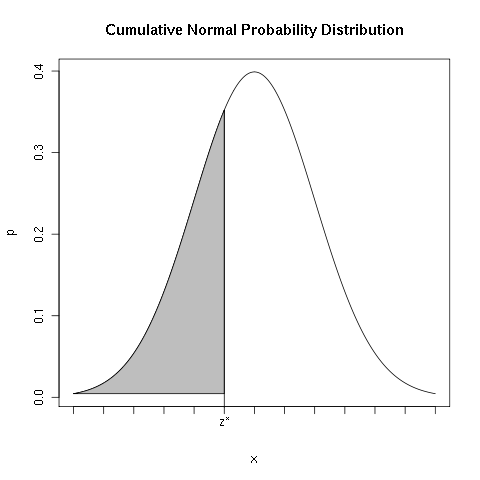
\includegraphics[width=2cm]{img/cummulativeDist}~~~~~~~~~~~~~~

  {
\fontencoding{T1}
\fontfamily{pcr}
\fontseries{m}
\fontshape{n}
\fontsize{5pt}{5pt}
\selectfont
\begin{tabular}{l|llllllllll}
     & 0.00   & 0.01   & 0.02   & 0.03   & 0.04   & 0.05   & 0.06   & 0.07   & 0.08  & 0.09 \\ \hline
0.0 & 0.5000 & 0.5040 & 0.5080 & 0.5120 & 0.5160 & 0.5199 & 0.5239 & 0.5279 & 0.5319 & 0.5359 \\ 
0.1 & 0.5398 & 0.5438 & 0.5478 & 0.5517 & 0.5557 & 0.5596 & 0.5636 & 0.5675 & 0.5714 & 0.5753 \\ 
0.2 & 0.5793 & 0.5832 & 0.5871 & 0.5910 & 0.5948 & 0.5987 & 0.6026 & 0.6064 & 0.6103 & 0.6141 \\ 
0.3 & 0.6179 & 0.6217 & 0.6255 & 0.6293 & 0.6331 & 0.6368 & 0.6406 & 0.6443 & 0.6480 & 0.6517 \\ 
0.4 & 0.6554 & 0.6591 & 0.6628 & 0.6664 & 0.6700 & 0.6736 & 0.6772 & 0.6808 & 0.6844 & 0.6879 \\ 
0.5 & 0.6915 & 0.6950 & 0.6985 & 0.7019 & 0.7054 & 0.7088 & 0.7123 & 0.7157 & 0.7190 & 0.7224 \\ 
0.6 & 0.7257 & 0.7291 & 0.7324 & 0.7357 & 0.7389 & 0.7422 & 0.7454 & 0.7486 & 0.7517 & 0.7549 \\ 
0.7 & 0.7580 & 0.7611 & 0.7642 & 0.7673 & 0.7704 & 0.7734 & 0.7764 & 0.7794 & 0.7823 & 0.7852 \\ 
0.8 & 0.7881 & 0.7910 & 0.7939 & 0.7967 & 0.7995 & 0.8023 & 0.8051 & 0.8078 & 0.8106 & 0.8133 \\ 
0.9 & 0.8159 & 0.8186 & 0.8212 & 0.8238 & 0.8264 & 0.8289 & 0.8315 & 0.8340 & 0.8365 & 0.8389 \\ 
1.0 & 0.8413 & 0.8438 & 0.8461 & 0.8485 & 0.8508 & 0.8531 & 0.8554 & 0.8577 & 0.8599 & 0.8621 \\ 
1.1 & 0.8643 & 0.8665 & 0.8686 & 0.8708 & 0.8729 & 0.8749 & 0.8770 & 0.8790 & 0.8810 & 0.8830 \\ 
1.2 & 0.8849 & 0.8869 & 0.8888 & 0.8907 & 0.8925 & 0.8944 & 0.8962 & 0.8980 & 0.8997 & 0.9015 \\ 
1.3 & 0.9032 & 0.9049 & 0.9066 & 0.9082 & 0.9099 & 0.9115 & 0.9131 & 0.9147 & 0.9162 & 0.9177 \\ 
1.4 & 0.9192 & 0.9207 & 0.9222 & 0.9236 & 0.9251 & 0.9265 & 0.9279 & 0.9292 & 0.9306 & 0.9319 \\ 
1.5 & 0.9332 & 0.9345 & 0.9357 & 0.9370 & 0.9382 & 0.9394 & 0.9406 & 0.9418 & 0.9429 & 0.9441 \\ 
1.6 & 0.9452 & 0.9463 & 0.9474 & 0.9484 & 0.9495 & 0.9505 & 0.9515 & 0.9525 & 0.9535 & 0.9545 \\ 
1.7 & 0.9554 & 0.9564 & 0.9573 & 0.9582 & 0.9591 & 0.9599 & 0.9608 & 0.9616 & 0.9625 & 0.9633 \\ 
1.8 & 0.9641 & 0.9649 & 0.9656 & 0.9664 & 0.9671 & 0.9678 & 0.9686 & 0.9693 & 0.9699 & 0.9706 \\ 
1.9 & 0.9713 & 0.9719 & 0.9726 & 0.9732 & 0.9738 & 0.9744 & 0.9750 & 0.9756 & 0.9761 & 0.9767 \\ 
2.0 & 0.9772 & 0.9778 & 0.9783 & 0.9788 & 0.9793 & 0.9798 & 0.9803 & 0.9808 & 0.9812 & 0.9817 \\ 
2.1 & 0.9821 & 0.9826 & 0.9830 & 0.9834 & 0.9838 & 0.9842 & 0.9846 & 0.9850 & 0.9854 & 0.9857 \\ 
2.2 & 0.9861 & 0.9864 & 0.9868 & 0.9871 & 0.9875 & 0.9878 & 0.9881 & 0.9884 & 0.9887 & 0.9890 \\ 
2.3 & 0.9893 & 0.9896 & 0.9898 & 0.9901 & 0.9904 & 0.9906 & 0.9909 & 0.9911 & 0.9913 & 0.9916 \\ 
2.4 & 0.9918 & 0.9920 & 0.9922 & 0.9925 & 0.9927 & 0.9929 & 0.9931 & 0.9932 & 0.9934 & 0.9936 \\ 
2.5 & 0.9938 & 0.9940 & 0.9941 & 0.9943 & 0.9945 & 0.9946 & 0.9948 & 0.9949 & 0.9951 & 0.9952 \\ 
2.6 & 0.9953 & 0.9955 & 0.9956 & 0.9957 & 0.9959 & 0.9960 & 0.9961 & 0.9962 & 0.9963 & 0.9964 \\ 
2.7 & 0.9965 & 0.9966 & 0.9967 & 0.9968 & 0.9969 & 0.9970 & 0.9971 & 0.9972 & 0.9973 & 0.9974 \\ 
2.8 & 0.9974 & 0.9975 & 0.9976 & 0.9977 & 0.9977 & 0.9978 & 0.9979 & 0.9979 & 0.9980 & 0.9981 \\ 
2.9 & 0.9981 & 0.9982 & 0.9982 & 0.9983 & 0.9984 & 0.9984 & 0.9985 & 0.9985 & 0.9986 & 0.9986 \\ 
3.0 & 0.9987 & 0.9987 & 0.9987 & 0.9988 & 0.9988 & 0.9989 & 0.9989 & 0.9989 & 0.9990 & 0.9990 \\ 
3.1 & 0.9990 & 0.9991 & 0.9991 & 0.9991 & 0.9992 & 0.9992 & 0.9992 & 0.9992 & 0.9993 & 0.9993 \\ 
3.2 & 0.9993 & 0.9993 & 0.9994 & 0.9994 & 0.9994 & 0.9994 & 0.9994 & 0.9995 & 0.9995 & 0.9995 \\ 
3.3 & 0.9995 & 0.9995 & 0.9995 & 0.9996 & 0.9996 & 0.9996 & 0.9996 & 0.9996 & 0.9996 & 0.9997 \\ 
3.4 & 0.9997 & 0.9997 & 0.9997 & 0.9997 & 0.9997 & 0.9997 & 0.9997 & 0.9997 & 0.9997 & 0.9998 
\end{tabular}

}

\end{frame}


\subsection{Standard Normal}

\begin{frame}{The Normal Distribution}

  \only<1>{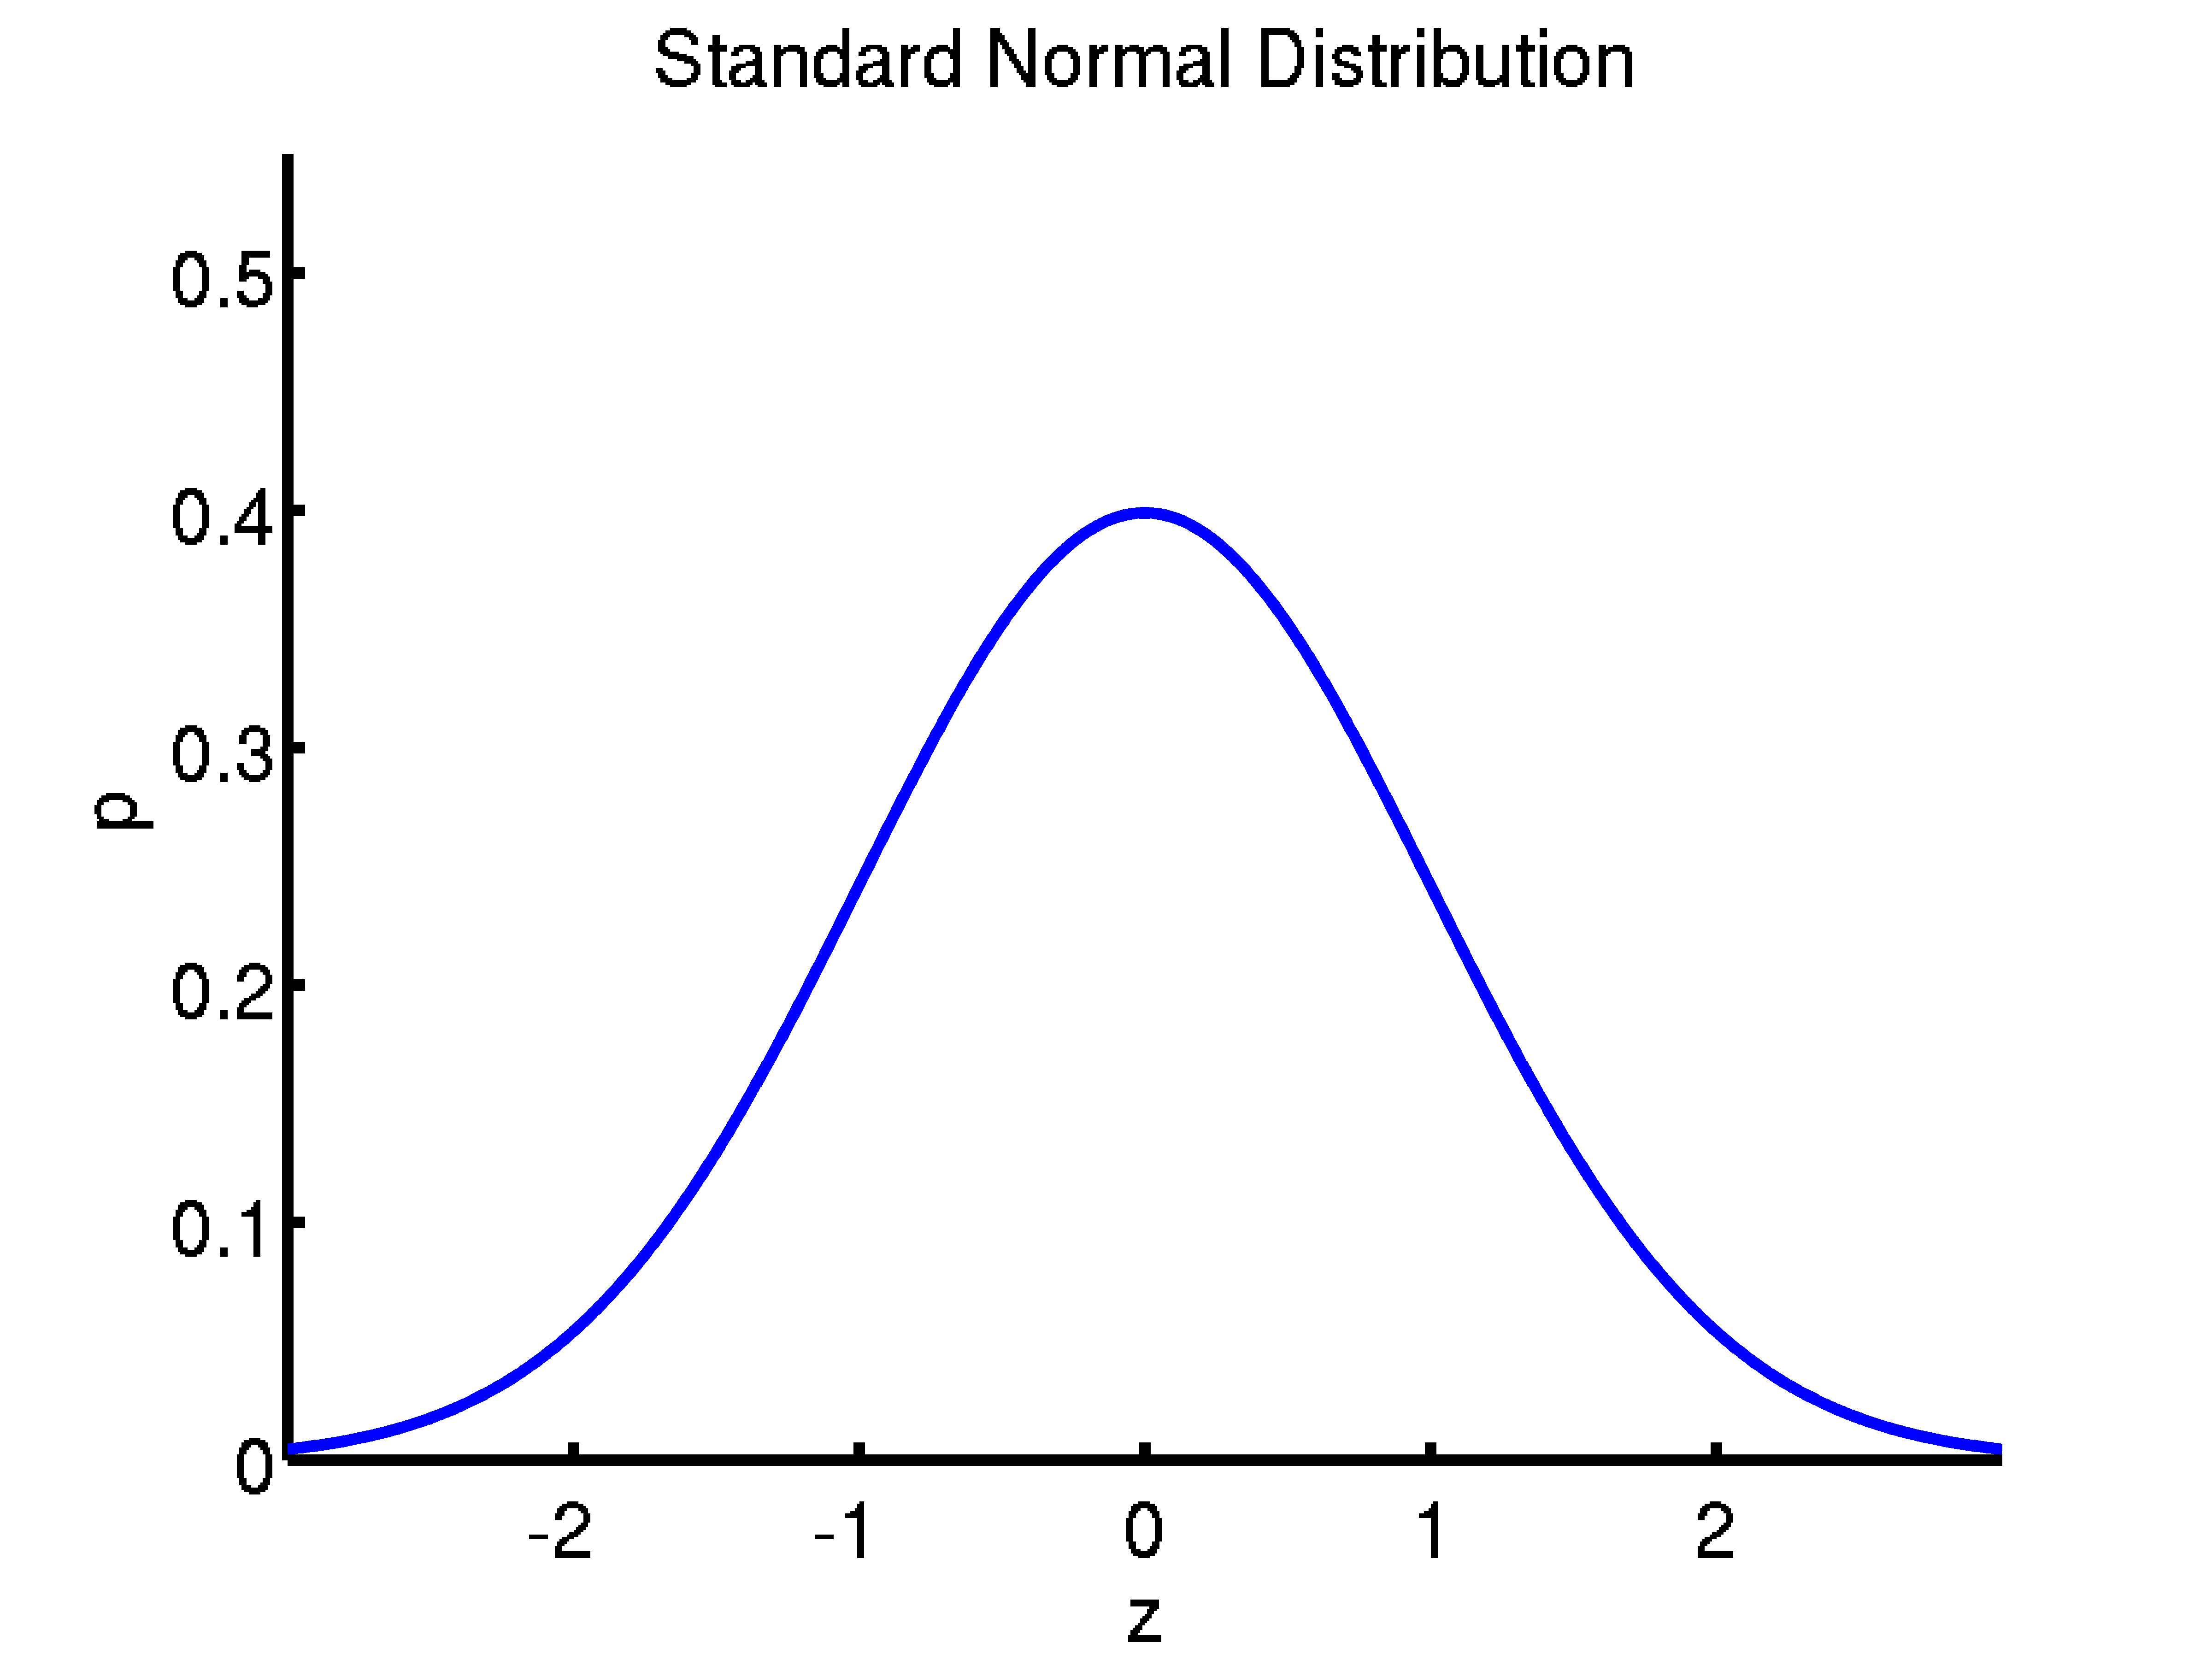
\includegraphics[width=5cm]{img/standardNormal}}
  \only<2>{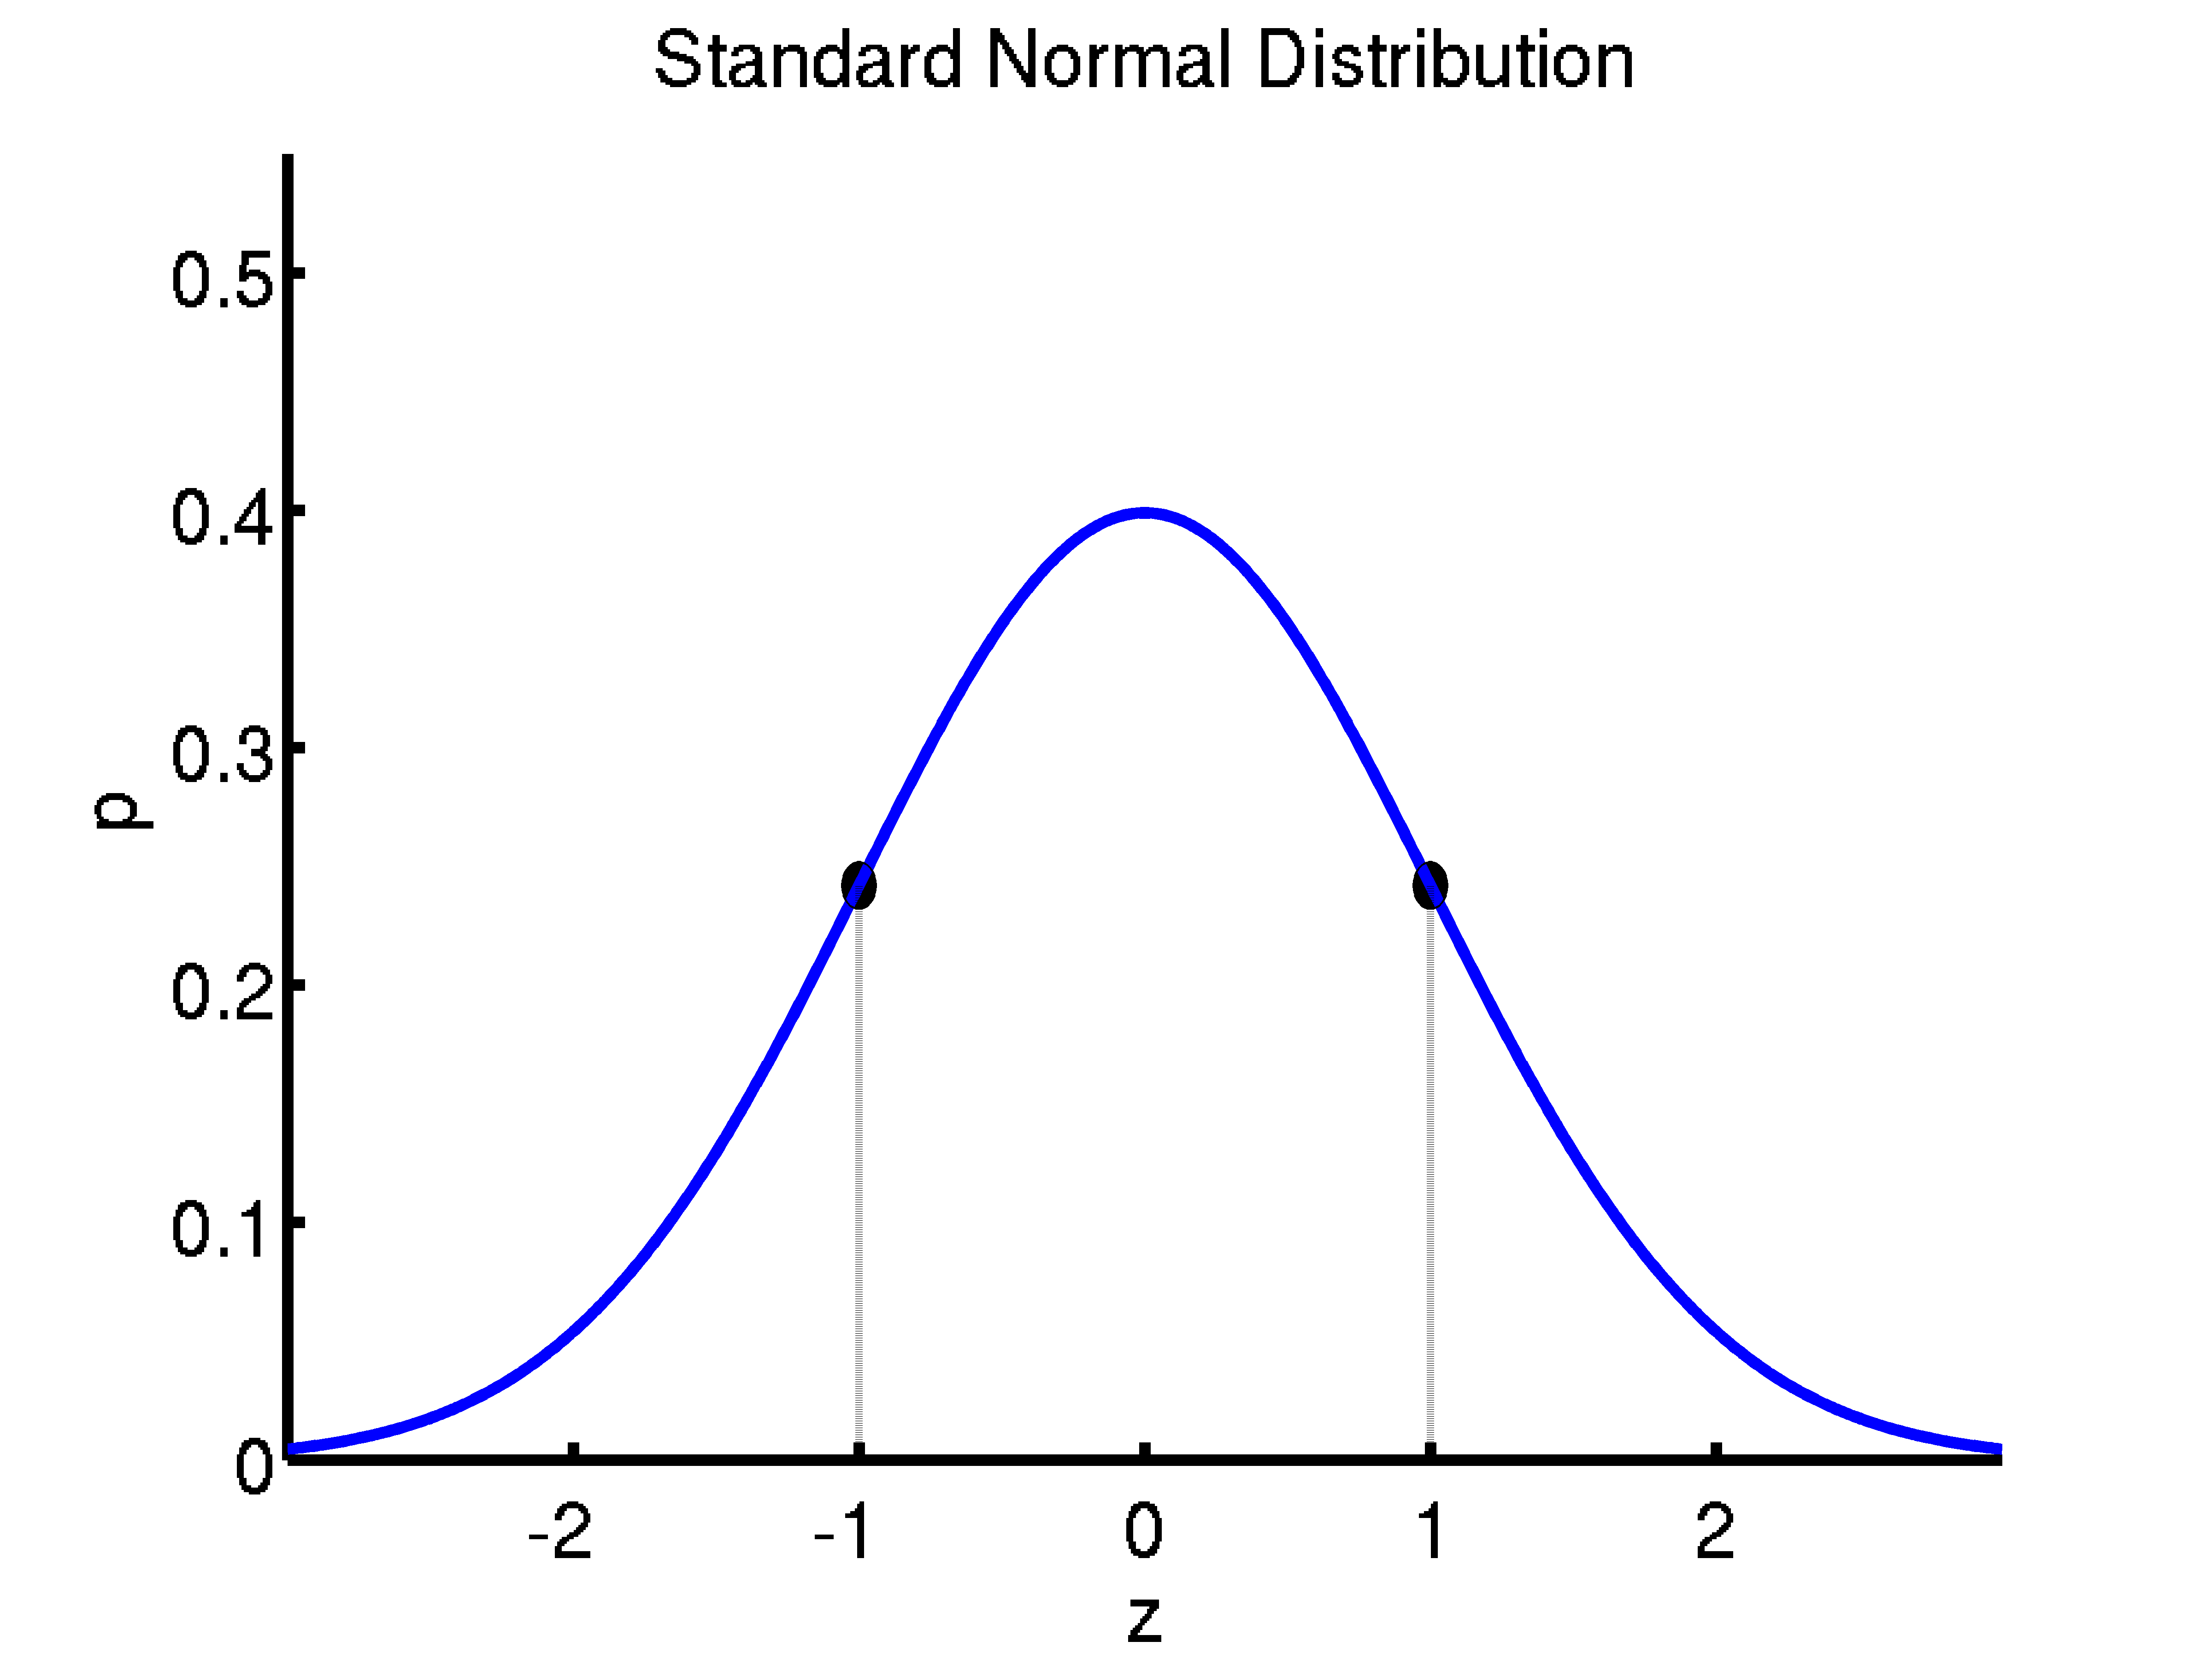
\includegraphics[width=5cm]{img/standardNormalInflection}}

  \begin{eqnarray*}
    f(z) & = & \frac{1}{\sqrt{2\pi}} e^{-z^2/2}.
  \end{eqnarray*}
  
\end{frame}

\begin{frame}{Probability and Area}

  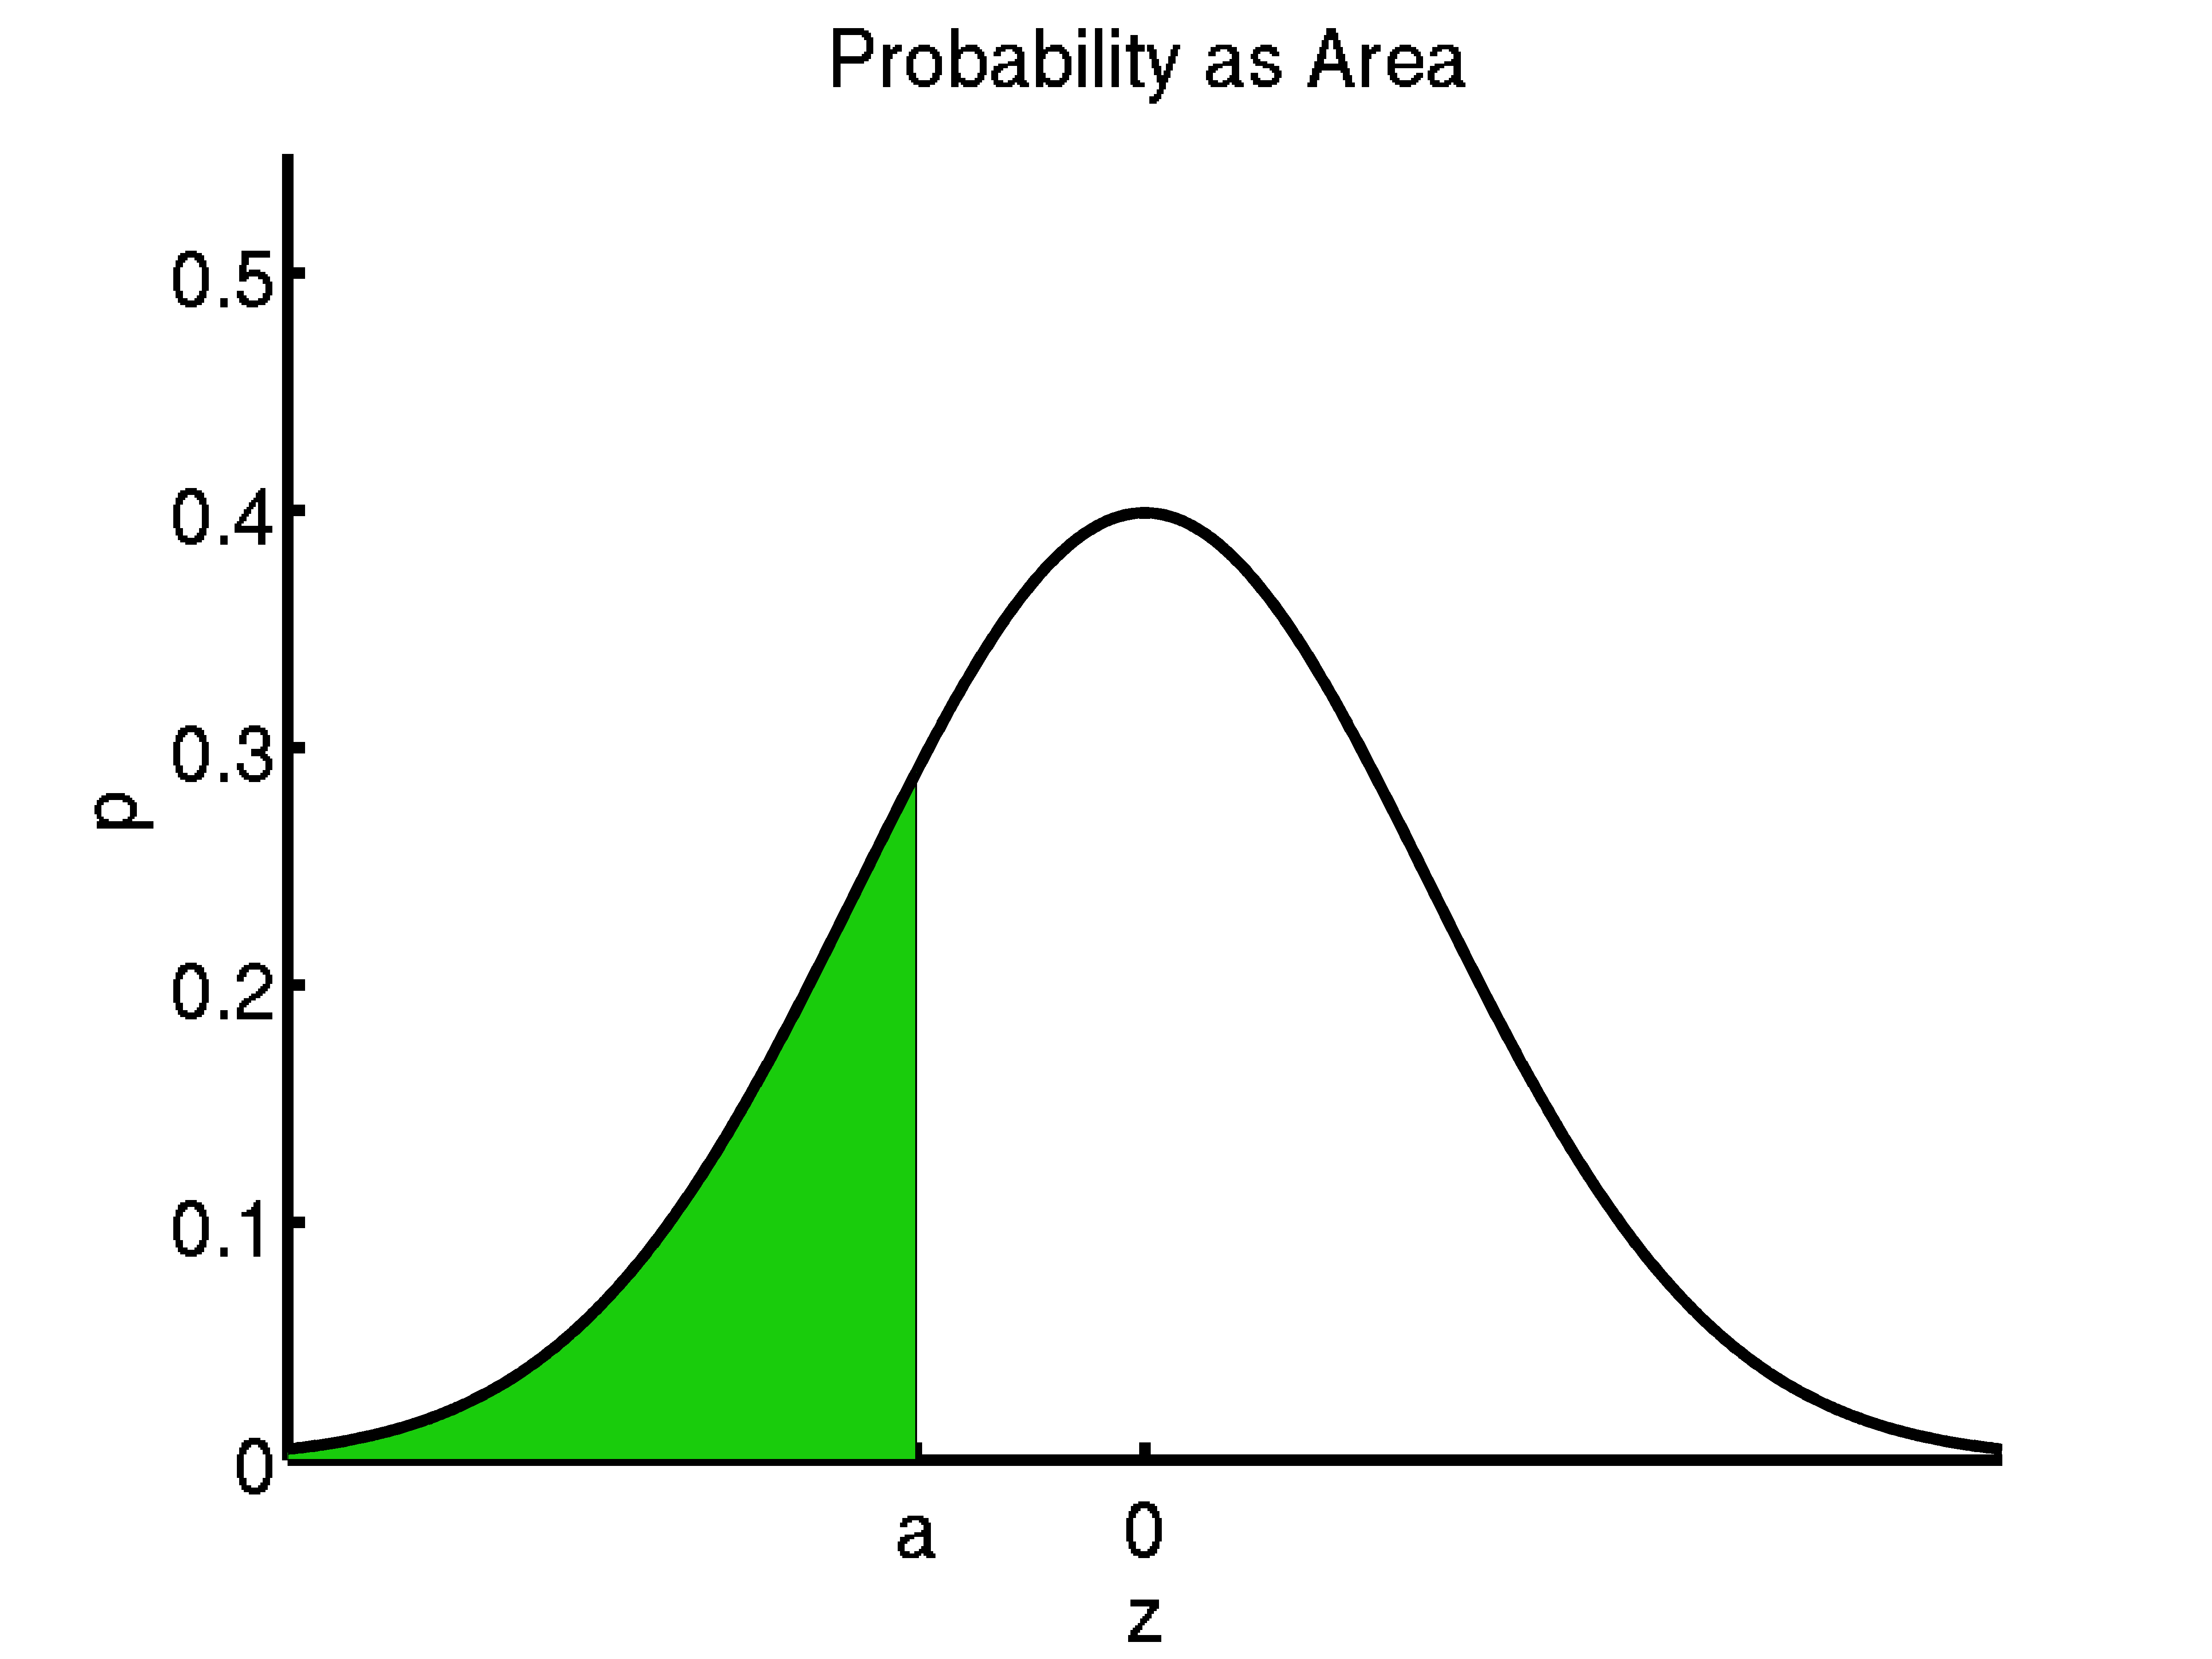
\includegraphics[width=5cm]{img/standardNormalArea}

  \begin{eqnarray*}
    p(X \leq a) 
  \end{eqnarray*}
  
\end{frame}


\begin{frame}{Probability and Area}

  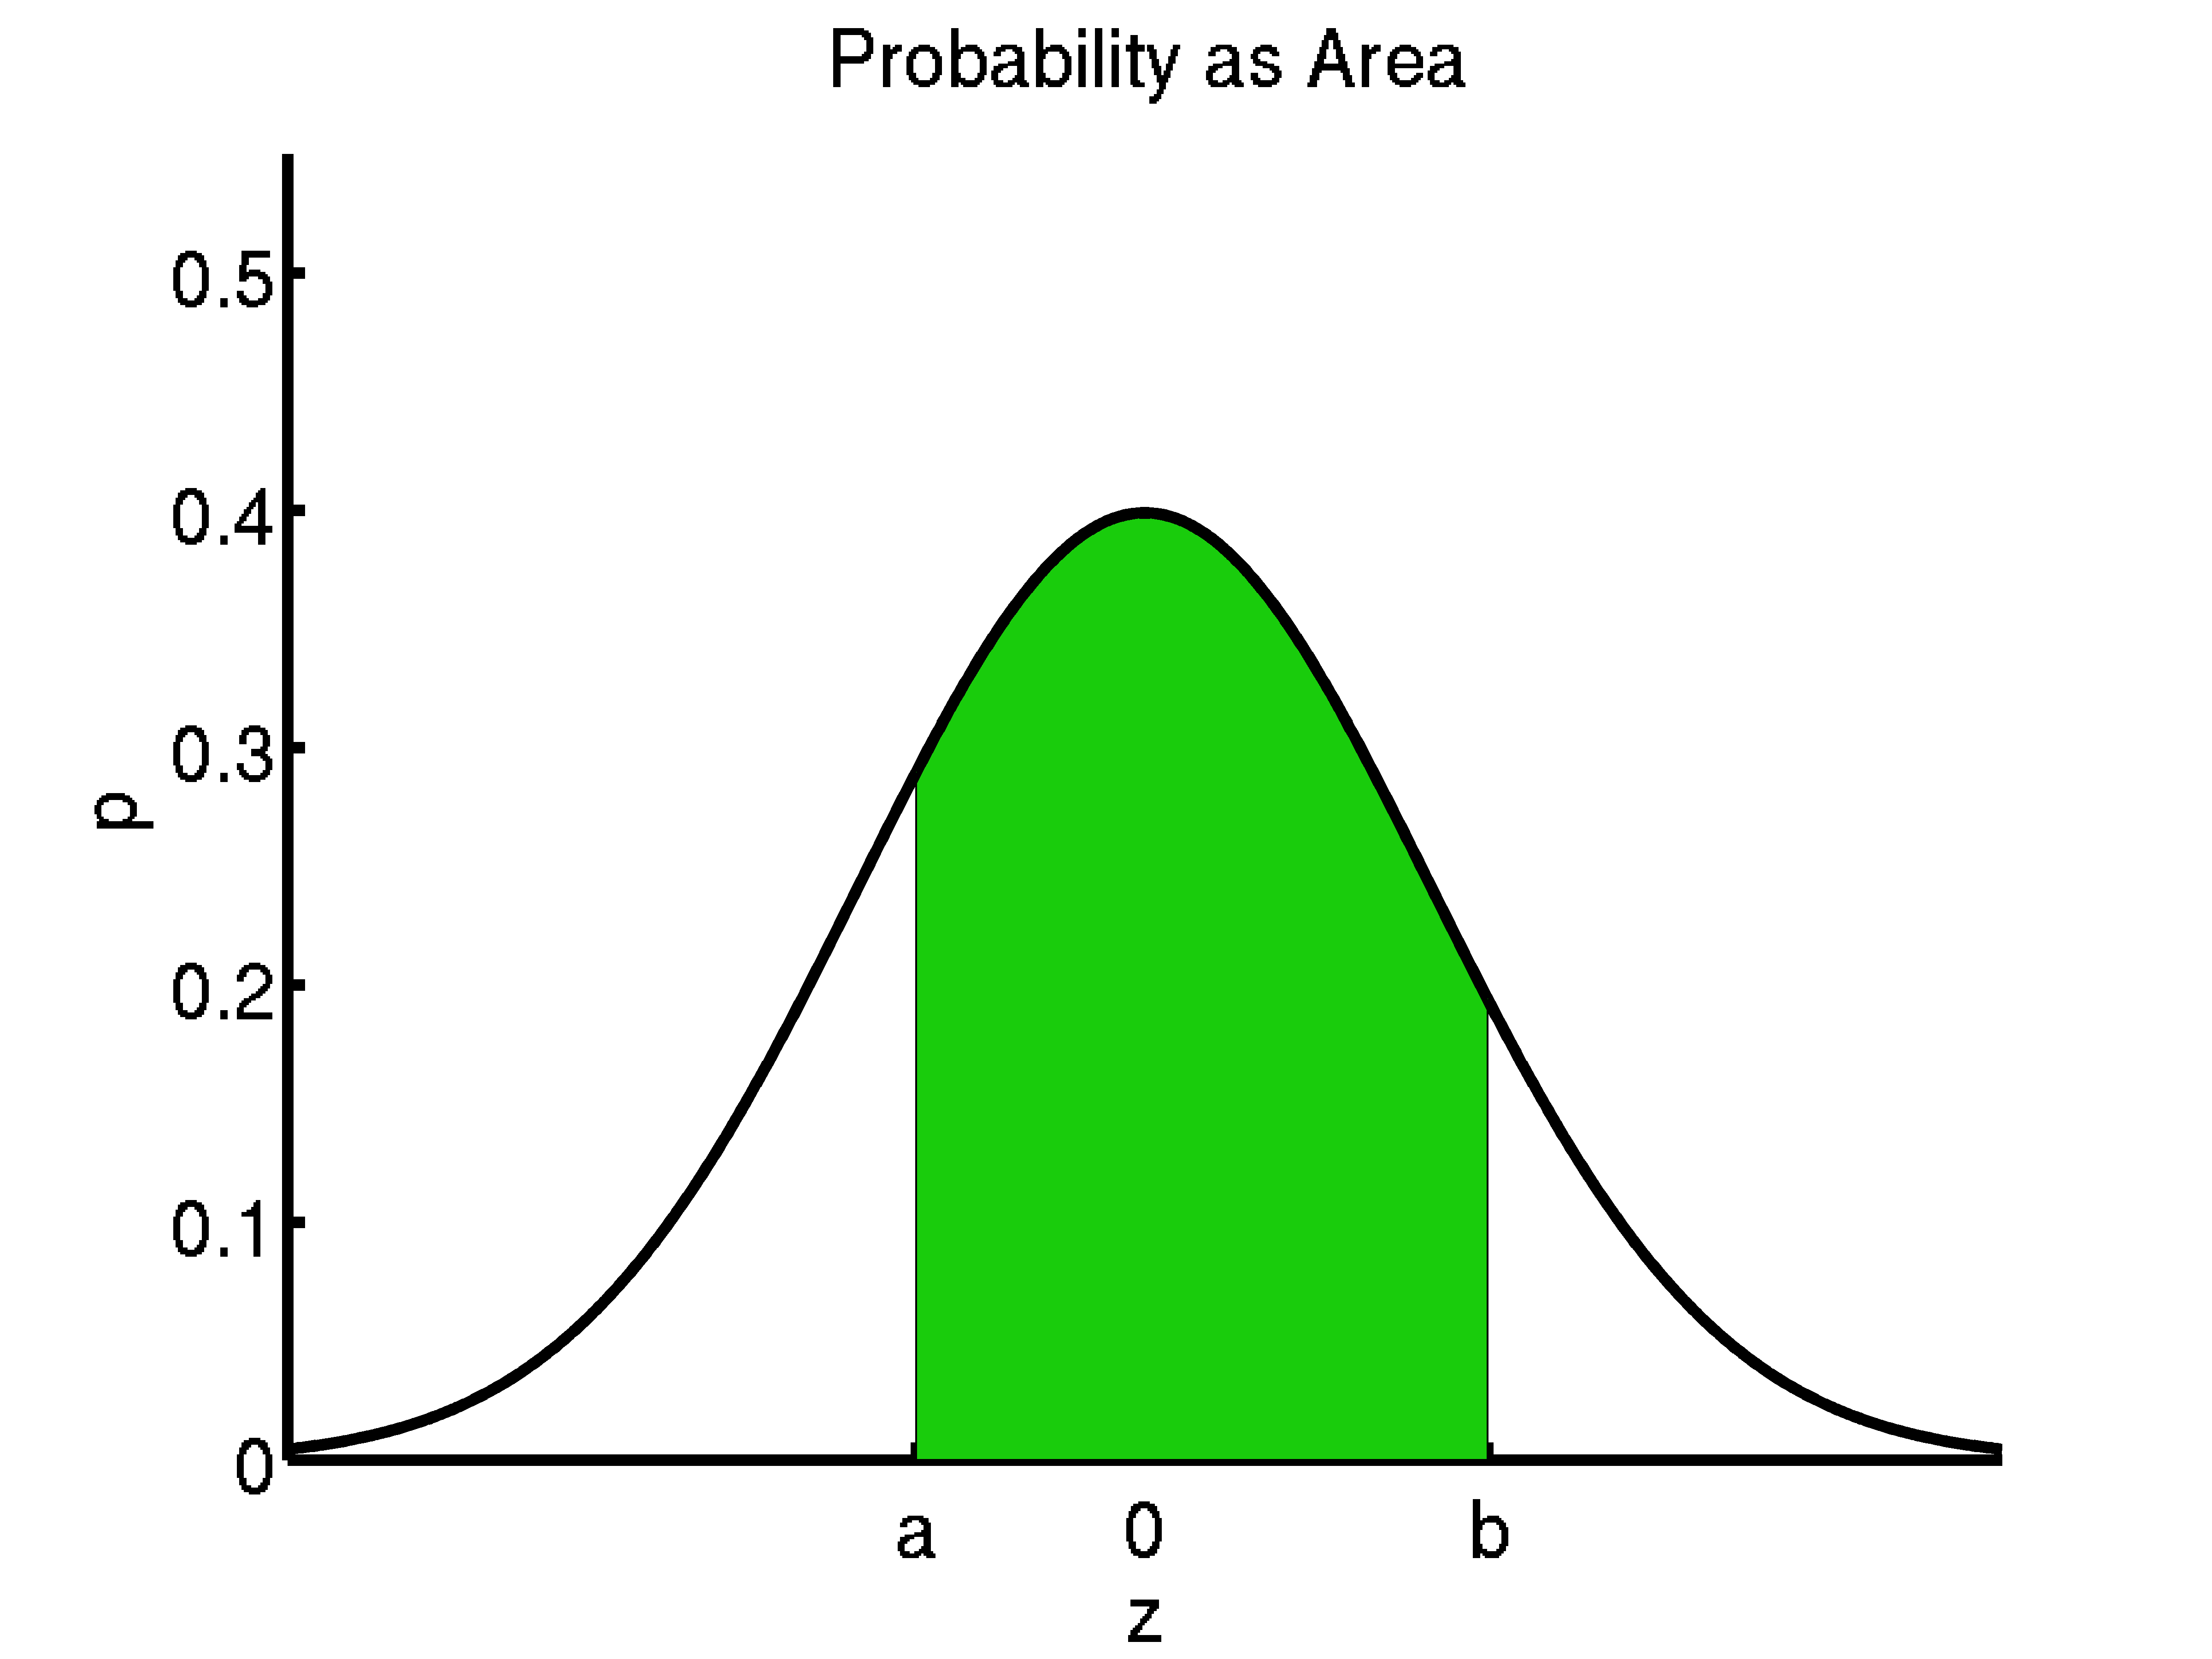
\includegraphics[width=5cm]{img/standardNormalAreaBoth}

  \begin{eqnarray*}
    p(a \leq X \leq b) 
  \end{eqnarray*}
  
\end{frame}


\begin{frame}{Example}

  What is the probability that a random variable that follows a
  standard normal is between -0.45 and 0.35?

  \vfill
  
\end{frame}


\begin{frame}{Work it backwards}

  Find the value, $z$, of a random variable that follows a standard normal
  so that the probability that it is less than $z$ is 0.35.

  \vfill
  
\end{frame}


\begin{frame}{Work it backwards}

  Find the value, $z$, of a random variable that follows a standard normal
  so that the probability that it is more than $z$ is 0.35.

  \vfill
  
\end{frame}



\subsection{General Normal Distribution}

\begin{frame}{General Normal Distribution}

  \begin{definition}
    If a random variable, $X$, is normally distributed with a mean
    $\mu$ and a standard deviation $\sigma$ then
    \begin{eqnarray*}
      Z & = & \frac{X-\mu}{\sigma}
    \end{eqnarray*}
    is a random variable that follows the standard normal
    distribution.
  \end{definition}
  
\end{frame}

\subsection{Examples}

\begin{frame}
  \frametitle{Example}

  A random variable, $X$, is normally distributed with a mean of 3.0
  and a standard distribution of 0.5. What is the probability that it
  is less than 2.4?

  \vfill

\end{frame}


\begin{frame}
  \frametitle{Example}

  A random variable, $X$, is normally distributed with a mean of 0.1
  and a standard distribution of 3.1. What is the probability that it
  is between -0.5 and 2.1?

  \vfill


\end{frame}




\iftoggle{clicker}{%
  \begin{frame}
    \frametitle{Clicker Quiz}

    A random variable, $X$, is normally distributed with a mean of 2.3
    and a standard distribution of 3.18. What is the probability that
    it is between -1.0 and 0.0?

    (Use the closest number)

    \vfill

 
    \begin{tabular}{l@{\hspace{3em}}l@{\hspace{3em}}l@{\hspace{3em}}l}
      A: 0.0569 & B: 0.0866  & C:   0.1073 & D: .3413 
    \end{tabular}

    \vfill
    \vfill
    \vfill


  \end{frame}
}



\begin{frame}{Example}

  A random variable, $X$, is normally distributed with mean -1.2 and a
  standard deviation of 4.5. Find the value of $X$ for which there is
  a probability of 0.25 to be less than that value.
  
\end{frame}





% LocalWords:  Clarkson pausesection hideallsubsections


\lecture{Examples of the Normal Distribution}{normal-distributions-examples}
\section{Examples of the Normal Distribution}

\title{Examples of the Normal Distribution}
\subtitle{Moar Normal!}

%\author{Kelly Black}
%\institute{Clarkson University}
\date{31 January 2014}

\begin{frame}
  \titlepage
\end{frame}

\begin{frame}
  \frametitle{Outline}
  \tableofcontents[hideothersubsections,sectionstyle=show/hide]
\end{frame}


\subsection{Clicker Quiz}


\iftoggle{clicker}{%
  \begin{frame}{Clicker Quiz}

    What is the probability that a random variable that follows a
    standard normal will be less than -0.45?

    \vfill

    \begin{tabular}{l@{\hspace{3em}}l@{\hspace{3em}}l}
      A:  .3264  & B: .3632  & C: .6736
    \end{tabular}

    \vfill
    \vfill
    \vfill

  \end{frame}
}


\subsection{Examples}

\begin{frame}
  \frametitle{Example}

  You are examining a portfolio of stocks. The total change in the
  value of an individual stock is normally distributed with a mean of
  0.5 and a standard deviation of 4.4. You want to decide which ones
  are in the top 25\% in gains based solely on the price change. What
  is the cut off?

  \vfill

  \only<2->{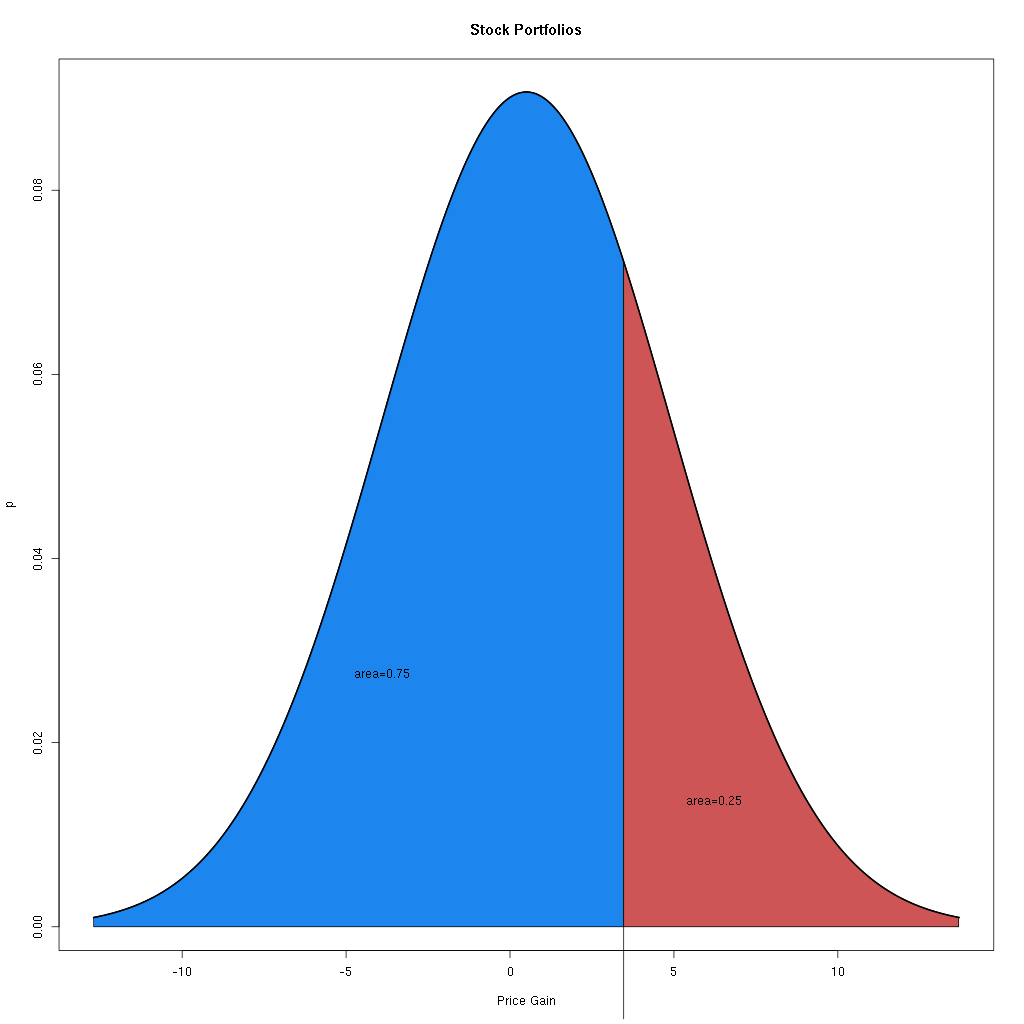
\includegraphics[width=12em]{img/topStockPicks}}

  \vfill


\end{frame}





\begin{frame}
  \frametitle{Example}

  A random variable has a mean of 3.0 and a standard deviation of
  4.5. If I take one sample what is the probability that it is less
  than zero?

  \vfill

  \only<2->{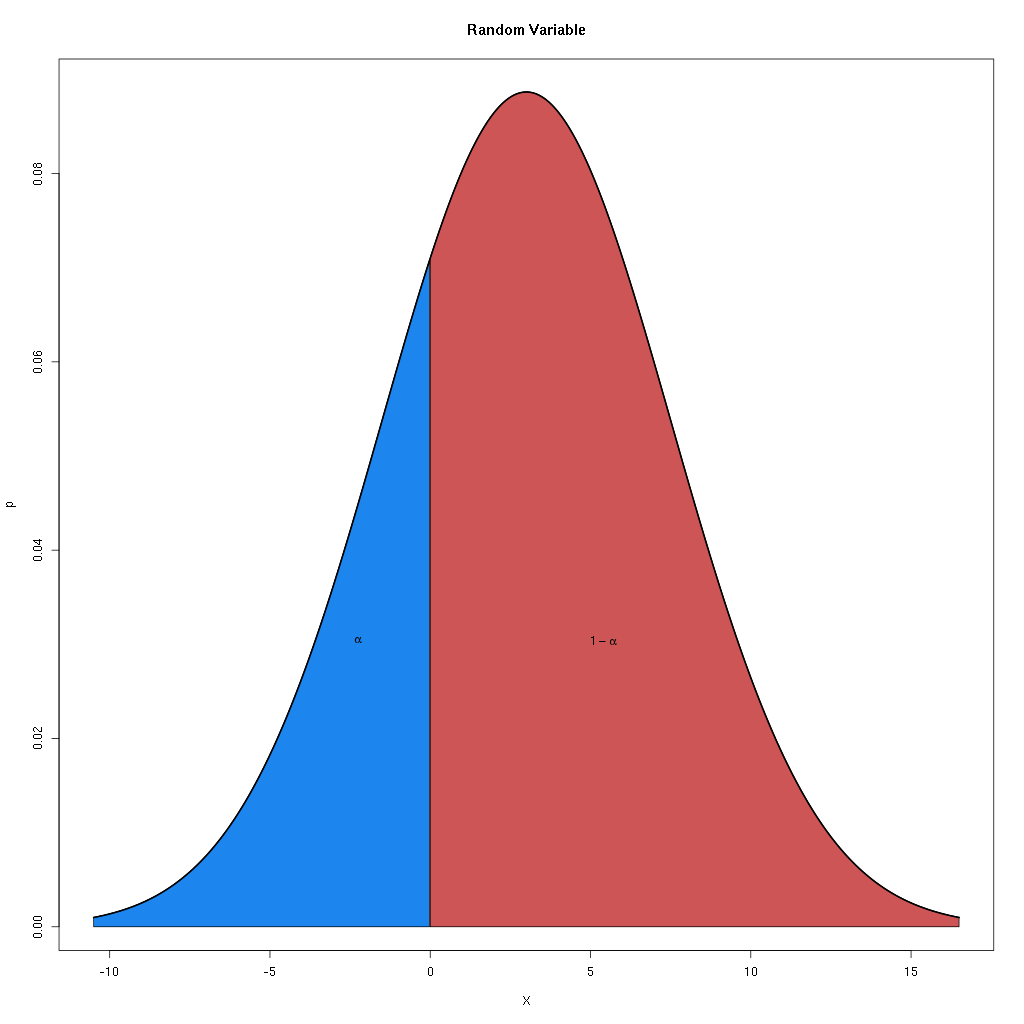
\includegraphics[width=12em]{img/normalRVMean3}}

  \vfill

%  \only<2->
%  {
%    If I take four samples what is the probability that it is less
%    than zero?
%  }
%
%  \vfill

\end{frame}

\iftoggle{clicker}{%
  \begin{frame}
    \frametitle{Clicker Quiz - Starting Salaries}

    The mean starting salaries for business majors is \$56,000 with a
    standard deviation of \$5,000. What is the probability that a
    randomly chosen business major will have an offer of more than
    \$63,000 per year?

    \vfill

    \begin{tabular}{l@{\hspace{3em}}l@{\hspace{3em}}l}
      A:  0.0808  & B: 0.919  & C: 1.4
    \end{tabular}

    \vfill
    \vfill
    \vfill



  \end{frame}
}





\iftoggle{clicker}{%
  \begin{frame}
    \frametitle{Clicker Quiz}

    The total change in a stock's price on one particular day has a
    mean of -.35\$ with a standard deviation of .86\$.  What is the
    probability that the price change in a randomly chosen stock will
    be more than zero?

    \vfill

    \begin{tabular}{l@{\hspace{3em}}l@{\hspace{3em}}l@{\hspace{3em}}l}
      A: 0.0516  & B: 0.3420 & C: 0.6580 & D: 0.9484
    \end{tabular}

    \vfill
    \vfill
    \vfill

  \end{frame}
}


\begin{frame}
  \frametitle{Example}

  A random variable has a mean of 12.0, and the probability that it is
  less than 8.0 is approximately 0.25. What is the standard deviation?

  \vfill

\end{frame}


\begin{frame}
  \frametitle{Example}

  A random variable has a mean of -2.0 and a standard deviation of
  5.0. Find the value, $x$, so that there is a probability of 0.30 that the
  random variable is bigger than than $x$.

  \vfill

\end{frame}




% LocalWords:  Clarkson pausesection hideallsubsections hideothersubsections
% LocalWords:  sectionstyle

% %%%%%%%%%%%%%%%%%%%%%%%%%%%%%%%%%%%%%%%%%%%%%%%%%%%%%%%%%%%%

\lecture{Introduction to Discrete}{introduction-to-discrete-data}
\section{Introduction to Discrete Data}

\title{Introduction to Discrete Data}
\subtitle{Quantitative Data}

%\author{Kelly Black}
%\institute{Clarkson University}
\date{2 February 2015}

\begin{frame}
  \titlepage
\end{frame}

\begin{frame}
  \frametitle{Outline}
  \tableofcontents[hideothersubsections,sectionstyle=show/hide]
\end{frame}


\iftoggle{clicker}{%
  \subsection{Clicker Quiz}
  \begin{frame}
    \frametitle{Clicker Quiz}

    The number of items produced per hour in a given factor is normally
    distributed with a mean of 230 items per hour and a standard
    deviation of 25 items per hour. What is the probability that in a
    given time period there will be more than 260 items per hour?

    \begin{tabular}{l@{\hspace{3em}}l@{\hspace{3em}}l@{\hspace{3em}}l}
      A:  0.0 & B: 0.1151  & C: 0.8849  & D: 1.20
    \end{tabular}


  \end{frame}
}





\subsection{Qualitative Data}

\begin{frame}{Qualitative Data}

  \begin{definition}{Discrete Data}

    A discrete random variable produces a countable number of
    values. The values are from a set of discrete values.
    
  \end{definition}

  \begin{definition}{Continuous Data}

    The numbers produced come from a continuous range of possible
    values.
    
  \end{definition}

  
\end{frame}


\begin{frame}{Discrete Data Examples}

  \begin{itemize}
  \item Someone reads an article, and we ask them to rate it on a
    scale: 1, 2, 3, 4, 5.

  \item We give a person three different soft drinks and ask them to
    tell us which one they like the best.

  \item We count the number of complaints that a department in a
    business receives over a preset period of time.

  \end{itemize}
  
\end{frame}

\subsection{Example}

\begin{frame}{The Data - An example}

  The people coming into a local drug store are monitored to see where
  people go to make a purchase. The following data is found: \\
  \begin{tabular}{l}
    Health Care \\
    Health Care \\
    Photo \\
    Candy \\
    Health Care \\
    Cosmetics \\
    Health Care \\
    Candy \\
    Health Care \\
    Cosmetics \\
    Cosmetics \\
    Health Care \\
    Photo 
  \end{tabular}

  How do we analyze this?
  
\end{frame}


\subsection{Frequency}

\begin{frame}{Frequencies}

  One way is to count the number of occurrences: \\
  \only<1>
  {
    \begin{tabular}{l}
      Health Care \\
      Health Care \\
      Photo \\
      Candy \\
      Health Care \\
      Cosmetics \\
      Health Care \\
      Candy \\
      Health Care \\
      Cosmetics \\
      Cosmetics \\
      Health Care \\
      Photo 
    \end{tabular}
  }


  \only<2>
  {
    \begin{tabular}{l|l}
      Department  & Frequency \\ \hline
      Health Care & 6 \\
      Photo       & 2 \\
      Candy       & 2 \\
      Cosmetics   & 3 \\
    \end{tabular}
  }


  \only<3>
  {
    \begin{tabular}{l|l}
      Department  & Relative Frequency \\ \hline
      Health Care & 6/13 \\
      Photo       & 2/13 \\
      Candy       & 2/13 \\
      Cosmetics   & 3/13 \\
    \end{tabular}
  }

  
\end{frame}


\subsection{Graphical Views of Discrete Data}

\begin{frame}{Graphical Views of the Data}

  The data can be viewed as a bar plot.

  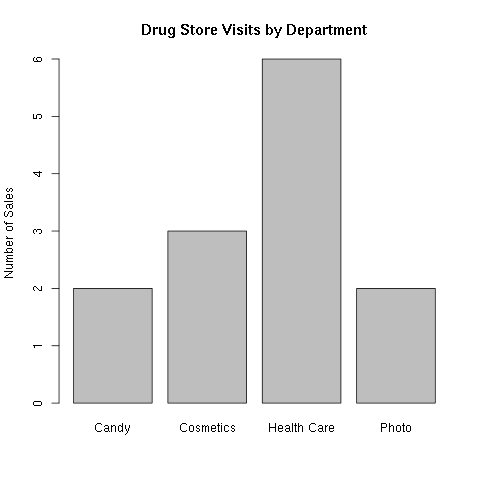
\includegraphics[width=6cm]{img/drugStoreBarPlot}
  
\end{frame}

\begin{frame}{Graphical Views of the Data}

  The data can be viewed as a Pareto plot.

  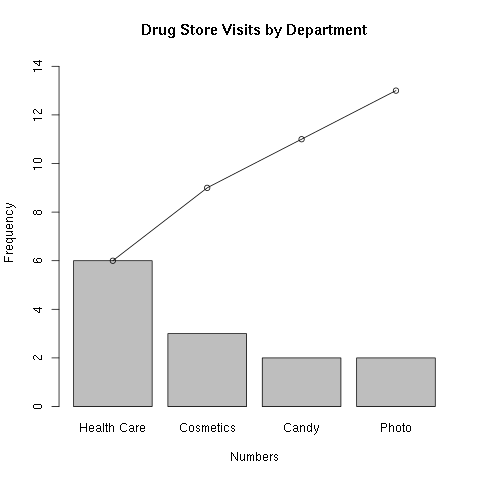
\includegraphics[width=6cm]{img/drugStorePareto}
  
\end{frame}


\iftoggle{clicker}{%
  \begin{frame}
    \frametitle{Clicker Quiz}

    Which plot below represents the Pareto chart for the following data:

    A, A, C, B, B, B, D

    \begin{tabular}{ccc}
      A: 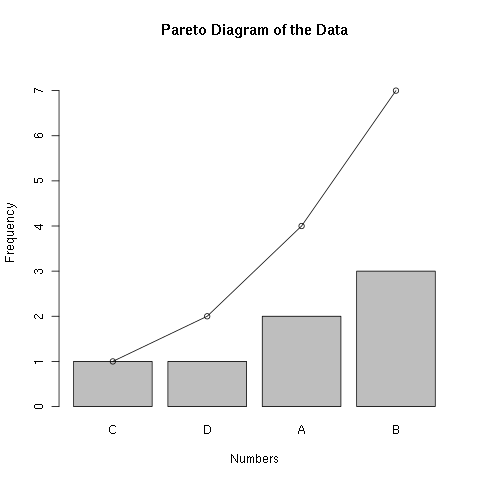
\includegraphics[width=3cm]{img/paretoQuizW1D2-a} &
      B: 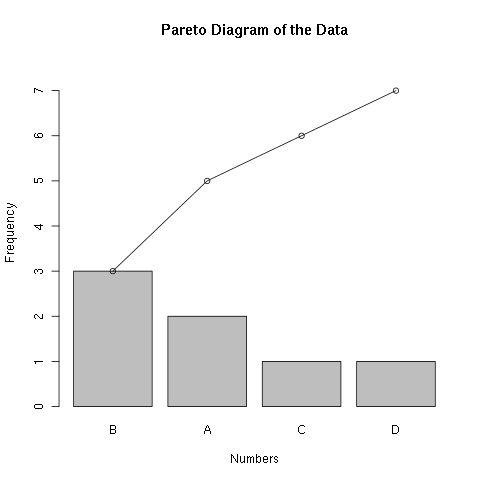
\includegraphics[width=3cm]{img/paretoQuizW1D2-b} &
      C: 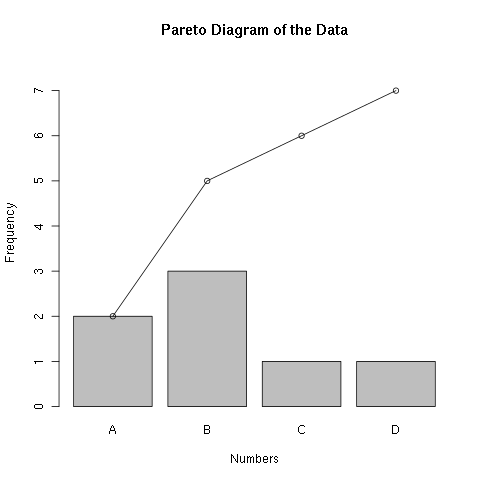
\includegraphics[width=3cm]{img/paretoQuizW1D2-c}
    \end{tabular}

  \end{frame}
}


\begin{frame}
  \frametitle{Cross Tabular Tables}


  \begin{columns}
    \column{.15\textwidth}

    \begin{tabular}{ll}
      $Q_{1}$ & $Q_{2}$ \\ \hline
      A & Y \\
      B & Y \\
      B & N \\
      B & N \\
      A & N \\
      A & N \\
      B & N
    \end{tabular}

    \column{.85\textwidth}

    \only<2->
    {
      \begin{tabular}{l|l|l|l}
        $Q_1 \backslash Q_2$ & Y & N & Row Total \\ \hline
        A & 1 & 2 & 3 \\ \hline
        B & 1 & 3 & 4 \\ \hline
        Col. Total & 2 & 5 & 7
      \end{tabular}
    }

  \end{columns}

    \vfill

    \only<3>
    {
      {\color{red}{Relative frequency}} \\
      \begin{tabular}{l|l|l|l}
        $Q_1 \backslash Q_2$ & Y & N & Row Total \\ \hline
        A & 0.14 & 0.29 & 0.43 \\ \hline
        B & 0.14 & 0.43 & 0.57 \\ \hline
        Col. Total & 0.29 & 0.71 & 1.0
      \end{tabular}
    }

    \vfill

    \only<4>
    {
      {\color{red}{Marginal Distribution by Rows}} \\
      \begin{tabular}{l|l|l|l}
        $Q_1 \backslash Q_2$ & Y & N & Relative Frequency\\ \hline
        A & 0.33 & 0.67 & 1.0 \\ \hline
        B & 0.25 & 0.75 & 1.0 \\ \hline
        Col. Total & 0.0.29 & 0.71 & 1.0
      \end{tabular}
    }

    \vfill

    \only<5>
    {
      {\color{red}{Marginal Distribution by Columns}} \\
      \begin{tabular}{l|l|l|l}
        $Q_1 \backslash Q_2$ & Y & N & Row Total \\ \hline
        A & 0.50 & 0.40 & 0.43 \\ \hline
        B & 0.50 & 0.60 & 0.57 \\ \hline
        Col. Total & 1 & 1 & 1
      \end{tabular}
    }


\end{frame}


\iftoggle{clicker}{%
  \begin{frame}
    \frametitle{Clicker Quiz}


    Determine the table for this data with the row percentages (Marginal Distribution by Rows):

    \begin{columns}
      \column{.25\textwidth}

      \begin{tabular}{l|l}
        $Q_{1}$ & $Q_{2}$ \\ \hline
        a & d \\
        a & e \\
        b & e \\
        a & d \\
        b & e \\
        a & d
      \end{tabular}


      \column{.75\textwidth}

      1:
      \begin{tabular}{l|l|l|l}
        $Q_1 \backslash Q_2$ & d & e & Row \\
        a & 3/4 & 1/4 & 1.0 \\ \hline
        b & 0.0 & 1.0 & 1.0 \\ \hline
        Col.  & 3/6 & 3/6 & 1.0
      \end{tabular}

      \rule{5cm}{0.05cm}

      2:
      \begin{tabular}{l|l|l|l}
        $Q_1 \backslash Q_2$ & d & e & Row  \\
        a & 1.0 & 1/3 & 4/6 \\ \hline
        b & 0.0 & 2/3 & 2/6 \\ \hline
        Col.  & 1.0 & 1.0 & 1.0
      \end{tabular}

      \rule{5cm}{0.05cm}

      3:
      \begin{tabular}{l|l|l|l}
        $Q_1 \backslash Q_2$ & d & e & Row  \\
        a & 1.0 & 0.0 & 1.0 \\ \hline
        b & 1/3 & 2/3 & 1.0 \\ \hline
        Col.  & 3/5 & 2/5 & 1.0
      \end{tabular}


    \end{columns}

  \end{frame}
}


\begin{frame}{Pie Charts}

  Pie charts are bad, bad, bad. People who use them have low
  self-esteem, poor personal hygiene and no friends. Do not let this
  happen to you.

  \vfill

  \centerline{
\includegraphics[width=4cm]{img/grumpyPieChart}}

  %\tiny{Just say'n}
  
\end{frame}

% LocalWords:  Clarkson pausesection hideallsubsections Bivariate


\lecture{Introduction to Bivariate Data}{introduction-to-bivariate-data}
\section{Introduction to Bivariate Data}

\title{Quantitative Data}
\subtitle{Methods to Assess Numerical Data}

%\author{Kelly Black}
%\institute{Clarkson University}
\date{8 February 2013}

\begin{frame}
  \titlepage
\end{frame}

\begin{frame}
  \frametitle{Outline}
  \tableofcontents[pausesection,hideothersubsections,sectionstyle=show/hide]
\end{frame}


\subsection{Clicker Quiz}


\iftoggle{clicker}{%
  \begin{frame}
    \frametitle{Clicker Quiz}

    A random variable is normally distributed with a mean of 1.2 and a
    standard deviation of 2.5. What is the probability that it is
    larger than 3.0?
    
    \vfill

    \begin{tabular}{l@{\hspace{3em}}l@{\hspace{3em}}l@{\hspace{3em}}l}
      A: 0.236 & B: 0.720  & C: 0.764 & D: 0.999
    \end{tabular}

    \vfill

  \end{frame}
}


\subsection{Quantitative Data}

\begin{frame}{Quantitative Data}
  
  \begin{definition}{Discrete Data}

    A discrete random variable produces a countable number of
    values. The values are one of a fixed set of values. 

    \textit{{\color{red}Here the random variables are numbers.}}
    
  \end{definition}

  \begin{definition}{Continuous Data}

    The numbers produced come from an infinite number of possible
    outcomes.
    
  \end{definition}

\end{frame}

\begin{frame}{Discrete Data Examples}

  \begin{itemize}
  \item Count the number of people who arrive in a line during a given
    time period.

  \item We report the number of bottles of a brand of soft drink that
    are sold in a given time period.

  \item We report the number of defects found in a mirror randomly
    chosen from a factory floor.

  \end{itemize}
  
\end{frame}


\begin{frame}{Quantitative Data}
  
  \begin{definition}{Univariate Data}

    The data consists of a set of numbers, and there are no explicit
    relationships between them.

    \textit{{\color{red}All of the examples on the previous slide
        represent univariate data.}}
    
  \end{definition}

  \begin{definition}{Bivariate Data}

    The data consists of pairs of numbers, and the pairs have some
    assumed relationship to one another.
    
  \end{definition}

  \begin{definition}{Multivariate Data}

    The data consists of groups of numbers, and the groups have some
    assumed relationship to one another. There is more than two
    numbers per group.
    
  \end{definition}


\end{frame}



\subsection{Bivariate Data}

\begin{frame}
  \frametitle{Bivariate Data}

  \begin{eqnarray*}
    \begin{array}{l|l}
      x      & y \\ \hline 
      x_1    & y_1 \\
      x_2    & y_2 \\
      \vdots & \vdots \\
      x_n    & y_n
    \end{array}
  \end{eqnarray*}
\end{frame}



\iftoggle{clicker}{%
  \begin{frame}
    \frametitle{Clicker Quiz}

    An experiment is run in which an intersection is observed over
    twenty different two hour periods, and the number of people who do
    not stop at a stop sign is observed.

    What kind of data is this?

    \vfill

    \begin{tabular}{l@{\hspace{3em}}l@{\hspace{3em}}l@{\hspace{3em}}l}
      A: univariate, discrete & B: univariate, continuous  \\
      C: bivariate, discrete  & D: bivariate, continuous
    \end{tabular}

    \vfill



  \end{frame}
}

\subsection{Discrete Quantitative Data}

\begin{frame}
  \frametitle{Discrete Quantitative Data}

  \begin{eqnarray*}
    5,~5,~3,~5,~4,~3,~4,~1,~6,~3,~2,~1
  \end{eqnarray*}

  This is no different from what we did with qualitative data in our
  last session. Just count the number of occurrences and work with
  frequencies.


  \only<2->%
  {
    \begin{tabular}{l|l}
      Number  & Frequency \\ \hline
      1 & 2 \\
      2 & 1 \\
      3 & 3 \\
      4 & 2 \\
      5 & 3 \\
      6 & 1 
    \end{tabular}
  }

  \only<3->%
  {
    \textit{relative frequency, blah blah blah}
  }

\end{frame}

\subsection{Continuous Data}

\begin{frame}
  \frametitle{Continuous Data}

  \begin{itemize}
  \item Every day I measure the amount of precipitation over the
    previous 24 hours.

  \item I observe the price of a particular stock at the end of each day.
    \uncover<2->{\textit{\color{red}Well... technically this is discrete, but we
        pretend it is continuous.}}

  \item I measure the blood alcohol levels for people who have been
    pulled over each night in Potsdam, NY.
  \end{itemize}
\end{frame}

\subsection{Graphical Techniques}

\begin{frame}{Graphical Techniques}

  \begin{itemize}
  \item Bar Plots
  \item Dot Plots
  \item Stem-Leaf Charts
  \item histograms
  \end{itemize}
  
\end{frame}


\begin{frame}{Bar Plots}

  \begin{eqnarray*}
    5,~5,~3,~5,~4,~3,~4,~1,~6,~3,~2,~1
  \end{eqnarray*}


  \begin{columns}
    \column{.25\textwidth}


    \begin{tabular}{l|l}
      Number  & Frequency \\ \hline
      1 & 2 \\
      2 & 1 \\
      3 & 3 \\
      4 & 2 \\
      5 & 3 \\
      6 & 1 
    \end{tabular}

    \column{.75\textwidth}

    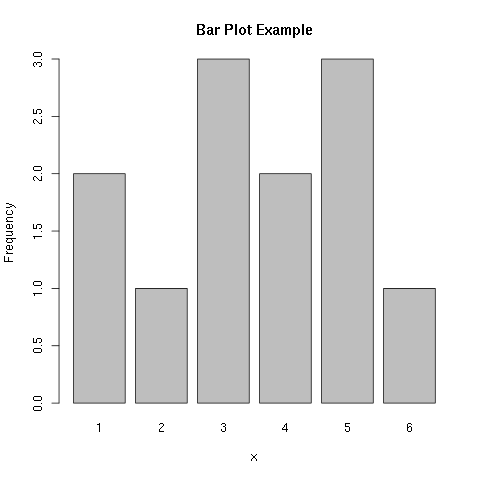
\includegraphics[width=7cm]{img/barplotExample}


  \end{columns}
  
  
\end{frame}


\begin{frame}{Dot Charts}

  \begin{eqnarray*}
    5,~5,~3,~5,~4,~3,~4,~1,~6,~3,~2,~1
  \end{eqnarray*}


  \begin{columns}
    \column{.25\textwidth}


    \begin{tabular}{l|l}
      Number  & Frequency \\ \hline
      1 & 2 \\
      2 & 1 \\
      3 & 3 \\
      4 & 2 \\
      5 & 3 \\
      6 & 1 
    \end{tabular}

    \column{.75\textwidth}

    \only<1>{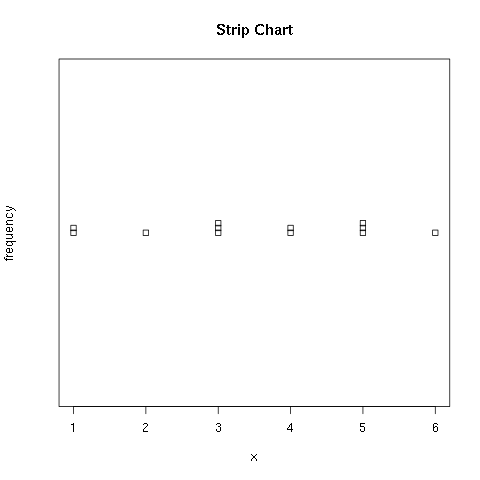
\includegraphics[width=7cm]{img/stripChart}}
    \only<2>{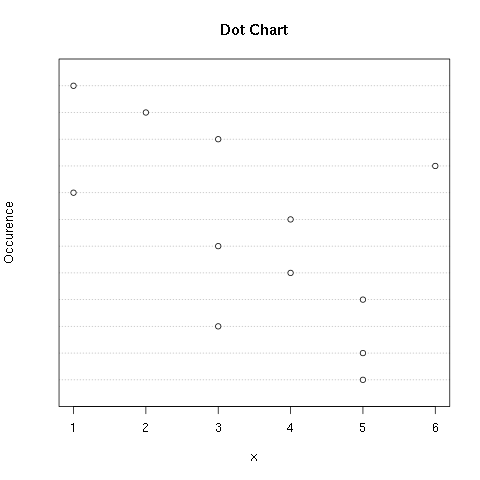
\includegraphics[width=7cm]{img/dotChart}}


  \end{columns}
  
  
\end{frame}


\begin{frame}{Stem-Leaf Plot}

  We can divide a number between its ``stem'' and ``leaf.''

  For example:
  \only<1>%
  {
    \begin{eqnarray*}
      17
    \end{eqnarray*}
  }
  \only<2>%
  {
    \begin{eqnarray*}
      \underbrace{\color{red}1}_{\mathrm{stem}}\underbrace{\color{blue}7}_{\mathrm{leaf}}
    \end{eqnarray*}
  }

  \only<3>%
  {
    Given a group of numbers we can organize the numbers with the same
    stem in the same rows. Then list each leaf in ascending order. The
    result is a ``stem-leaf plot.''
  }
  
  
\end{frame}

\begin{frame}{Example}

  \only<1>%
  {
    \begin{eqnarray*}
      47,~44,~29,~27,~29,~36,~24,~21,~36,~34
    \end{eqnarray*}
  }
  \only<2>%
  {
    Identify the stems:
    \begin{eqnarray*}
      {\color{red}4}7,~{\color{red}4}4,~{\color{red}2}9,~{\color{red}2}7,
      ~{\color{red}2}9,~{\color{red}3}6,~{\color{red}2}4,~{\color{red}2}1,
      ~{\color{red}3}6,~{\color{red}3}4
    \end{eqnarray*}
  }\
  \only<3->%
  {
    Identify the leaves:
    \begin{eqnarray*}
      {\color{red}4}{\color{blue}7},~{\color{red}4}{\color{blue}4},
      ~{\color{red}2}{\color{blue}9},~{\color{red}2}{\color{blue}7},
      ~{\color{red}2}{\color{blue}9},~{\color{red}3}{\color{blue}6},
      ~{\color{red}2}{\color{blue}4},~{\color{red}2}{\color{blue}1},
      ~{\color{red}3}{\color{blue}6},~{\color{red}3}{\color{blue}4}
    \end{eqnarray*}
  }

  \only<4>%
  {
    Write out the unique stems in order: \\
    \begin{tabular}{l@{\hspace{1em}}|@{\hspace{1em}}l}
      {\color{red}2} & \\
      {\color{red}3} & \\
      {\color{red}4} & 
    \end{tabular}
  }

  \only<5>%
  {
    Write out every leaf in ascending order: \\
    \begin{tabular}{l@{\hspace{1em}}|@{\hspace{1em}}l}
      {\color{red}2} & {\color{blue}14799}\\
      {\color{red}3} & {\color{blue}466}\\
      {\color{red}4} & {\color{blue}47}
    \end{tabular}
  }

  
\end{frame}

\begin{frame}{Histograms}

  This is a generalization of the stem-leaf plot. Instead of dividing
  things in groups by the ``tens'' we instead use an arbitrary range
  of values. We calculate how many data points fall into the
  pre-determined ranges and then make a bar plot of the frequencies.
  
\end{frame}

\begin{frame}{Example}

  \begin{eqnarray*}
    2.7,~3.6,~3.8,~2.7,~2.7,~3.3,~3.3,~3.6,~3.0,~3.2
  \end{eqnarray*}


  \begin{columns}
    \column{.25\textwidth}

    \only<2>%
    {
      We (arbitrarily) break things up into a range of values: \\
      \begin{tabular}{l|l}
        2.6-2.8 \\
        2.8-3.0 \\
        3.0-3.2 \\
        3.2-3.4 \\
        3.4-3.6 \\
        3.6-3.8
      \end{tabular}
    }

    \only<3->%
    {
      We (arbitrarily) break things up into a range of values: \\
      \begin{tabular}{l|l}
        2.6-2.8 & III\\
        2.8-3.0 & I \\
        3.0-3.2 & I \\
        3.2-3.4 & II \\
        3.4-3.6 & II \\
        3.6-3.8 & I
      \end{tabular}
    }
    
    \column{.75\textwidth}

    \only<4>{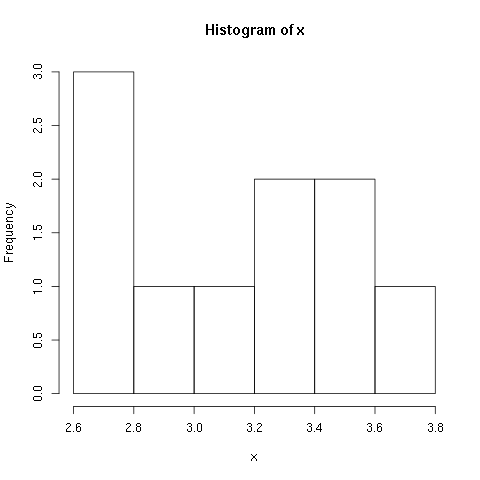
\includegraphics[width=6cm]{img/histogramExample}}

  \end{columns}

  
\end{frame}

\begin{frame}{Histograms}

  \begin{itemize}
  \item Overall shape 
  \item Skew
  \item Center (balance point, middle of area)
  \item Spread
  \end{itemize}
  
\end{frame}

% LocalWords:  Clarkson pausesection hideallsubsections Bivariate

% %%%%%%%%%%%%%%%%%%%%%%%%%%%%%%%%%%%%%%%%%%%%%%%%%%%%%%%%%%%%

\lecture{Point Estimates}{point-estimates}
\section{Point Estimates}

\title{Point Estimates}
\subtitle{Estimating Parameters}

%\author{Kelly Black}
%\institute{Clarkson University}
\date{18 October 2013}

\begin{frame}
  \titlepage
\end{frame}

\begin{frame}
  \frametitle{Outline}
  \tableofcontents[hideothersubsections,sectionstyle=show/hide]
\end{frame}


\iftoggle{clicker}{%
  \subsection{Clicker Question}
  \begin{frame}
    \frametitle{Find The Sample mean}
    (Use channel 42)

    \vfill 
    
    \begin{tabular}{lll}
      3, & 5, & -2
    \end{tabular}

    \vfill

    \begin{tabular}{l@{\hspace{3em}}l@{\hspace{3em}}l}
      a: -2 & b: 2 & c: 4
    \end{tabular}

    \vfill


  \end{frame}
}


\subsection{Point Estimates}

\begin{frame}{Point Estimates}

  We have a random variables and have samples of the random
  variable:\\ [10pt]
  \begin{tabular}{l|l}
    Observation & Value \\ \hline
    1 & $x_1$ \\ 
    2 & $x_2$ \\
    3 & $x_3$ \\
    \vdots & \vdots \\
    $n$ & $x_n$
  \end{tabular}

  \vfill

  What estimate can we make for a ``parameter?''

  \vfill
  
\end{frame}


\begin{frame}{Parameters versus Statistic}

  \begin{definition}[Parameter]
    A \redText{parameter} is a quantity that is a \blueText{property}
    of the random variable.
  \end{definition}

  \begin{definition}[Statistic]
    A \redText{statistic} is a \blueText{calculation} based on a set
    of samples.
  \end{definition}

\end{frame}




\begin{frame}
  \frametitle{Example}

  A random variable has a mean $\mu$ and standard deviation
  $\sigma$. A set of samples is taken: \\ [10pt]
  \begin{tabular}{l|l}
    Observation & Value \\ \hline
    1 & $1.0$ \\ 
    2 & $3.0$ \\
    3 & $8.0$ \\
    4 & $4.0$ \\
    5 & $7.0$
  \end{tabular}

\end{frame}


\begin{frame}{Point Estimate}

  \begin{definition}[Point Estimate]
    A \redText{point estimate} is an \blueText{estimate} of a
    parameter based on whatever, limited, information that is
    available to us.
  \end{definition}
\end{frame}


\begin{frame}{Example}

  $\bar{x}$ is an estimate for the mean.
  
\end{frame}

\begin{frame}{Example}
  How likely is it that a coin flip returns a tails?

  \vfill

  Flip a coin seven times.

  \vfill

\end{frame}


\begin{frame}{Example}

  The voltage difference across a resistor is measured at random
  times: \\ [10pt]
  \begin{tabular}{l|l}
    Observation & Voltage \\ \hline
    1 & 3.50 \\
    2 & 3.61 \\
    3 & 3.53 \\
    4 & 3.55 
  \end{tabular}
  
\end{frame}

\begin{frame}{Extra Examples}

  \vfill

  The following examples are extra examples that are not covered in
  class.

  \vfill
  
\end{frame}

\begin{frame}{Example}

  \begin{tabular}{lllllll}
    30 & 28 & 31 & 33 & 35 & 22 & 31
  \end{tabular}

  The sample mean:
  \begin{eqnarray*}
    \bar{x} & = & \frac{30 + 28 + 31 + 33 + 35 + 22 + 31}{7}, \\
    & = & 30.
  \end{eqnarray*}

  To get the median first order the data: \\
  \only<1>%
  {
    \begin{tabular}{lllllll}
      22 & 28 & 30 & 31 & 31 & 33 & 35
    \end{tabular}
  }

  \only<2>%
  {
    \begin{tabular}{lllllll}
      {\color{red}22} & {\color{red}28} & {\color{red}30} & 31 & {\color{blue}31} & {\color{blue}33} & {\color{blue}35}
    \end{tabular}
  }

  \only<3->%
  {
    \begin{tabular}{lllllll}
      {\color{red}22} & {\color{red}28} & {\color{red}30} & $\underbrace{31}_{Median}$ & {\color{blue}31} & {\color{blue}33} & {\color{blue}35}
    \end{tabular}
  }
  
\end{frame}


\begin{frame}{Example}

  Even number of data points.

  \begin{tabular}{lllllll}
    30 & 28 & 31 & 33 & 35 & 22 
  \end{tabular}

  The sample mean:
  \begin{eqnarray*}
    \bar{x} & = & \frac{30 + 28 + 31 + 33 + 35 + 22}{6}, \\
    & = & 29.8.
  \end{eqnarray*}

  To get the median first order the data: \\
  \only<1>%
  {
    \begin{tabular}{llllll}
      22 & 28 & 30 & 31 & 33 & 35
    \end{tabular}
  }

  \only<2>%
  {
    \begin{tabular}{llllll}
      {\color{red}22} & {\color{red}28} & 30 & 31  & {\color{blue}33} & {\color{blue}35}
    \end{tabular}
  }

  \only<3->%
  {
    \begin{tabular}{llccll}
      {\color{red}22} & {\color{red}28} & 30 & 31 & 
      {\color{blue}33} & {\color{blue}35} \\
      & & \multicolumn{2}{c}{Median = $\frac{30+31}{2}$} 
    \end{tabular}
  }
  
\end{frame}


\begin{frame}
  \frametitle{Clicker Quiz}
  (Use channel 42)

  Find the median of the following data set:
  \vfill 

  \begin{tabular}{llll}
    3, & 5, & 2, & 4
  \end{tabular}

  \vfill

  \begin{tabular}{l@{\hspace{3em}}l@{\hspace{3em}}l@{\hspace{3em}}l}
    a: 5/2  & b: 7/2 & c: 3 & D: 4
  \end{tabular}

  \vfill

  

\end{frame}

\begin{frame}{Why Two Measures?}

  \begin{enumerate}
  \item They represent different things.
  \item The median is more robust.
  \end{enumerate}

  \only<1-2>%
  {
    Example: \\
    \begin{tabular}{llllll}
      94 & 105 & 95 & 97  & 99 & 101
    \end{tabular}

    \only<2>%
    {
      The median is 98, and the mean is 98.5.
    }
  }

  \only<3-4>%
  {
    Alter the example: \\
    \begin{tabular}{llllll}
      94 & 105 & 95 & 97  & 99 & {\color{red}110}
    \end{tabular}

    \only<4>%
    {
      The median is 98, and the mean is 101.7. The median is less
      likely to be altered by outliers.
    }
  }

  
  
\end{frame}

\subsection{Skew}

\begin{frame}{Skew}

  \begin{definition}[Left Skew]
    If the mean is to the left of the median the data is skewed to the
    left.
  \end{definition}

  \begin{definition}[Right Skew]
    If the mean is to the right of the median the data is skewed to
    the right.
  \end{definition}

  \begin{definition}[Symmetric]
    If the mean is close to the median the data is symmetric.
  \end{definition}
  
\end{frame}

\begin{frame}{Skewed to the Left}

  \only<1>%
  {
    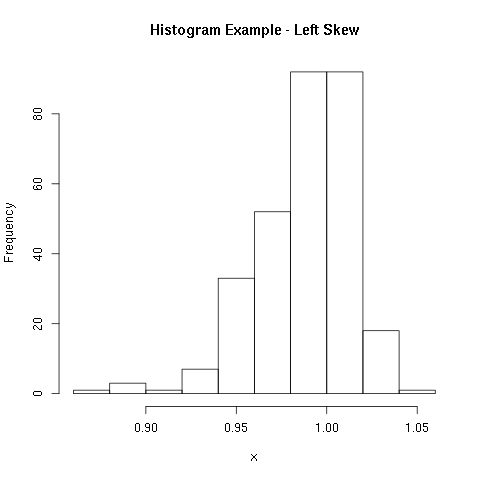
\includegraphics[width=7cm]{img/leftSkew}
  }

  \only<2>%
  {
    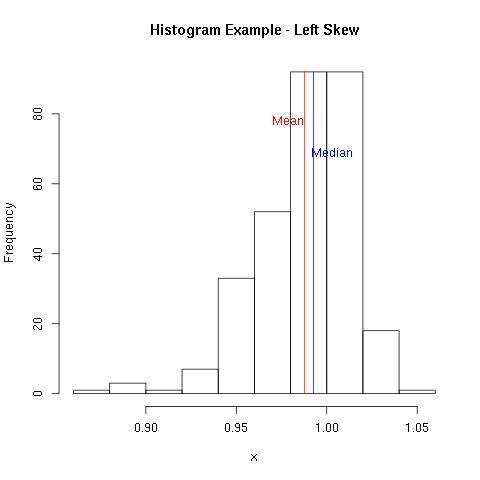
\includegraphics[width=7cm]{img/leftSkewAnnotated}
  }

  
\end{frame}


\begin{frame}{Skewed to the Right}

  \only<1>%
  {
    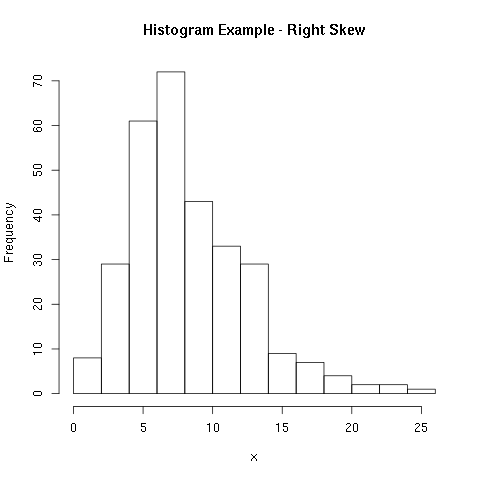
\includegraphics[width=7cm]{img/rightSkew}
  }

  \only<2>%
  {
    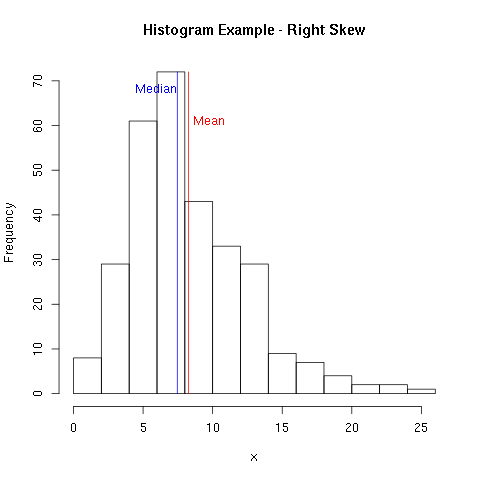
\includegraphics[width=7cm]{img/rightSkewAnnotated}
  }

  
\end{frame}


\begin{frame}{Symmetric}

  \only<1>%
  {
    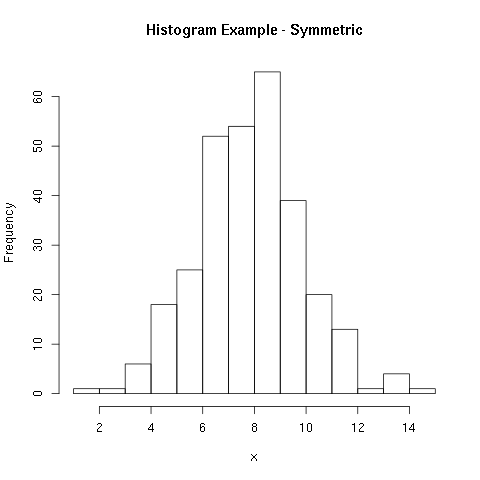
\includegraphics[width=7cm]{img/symmetric}
  }

  \only<2>%
  {
    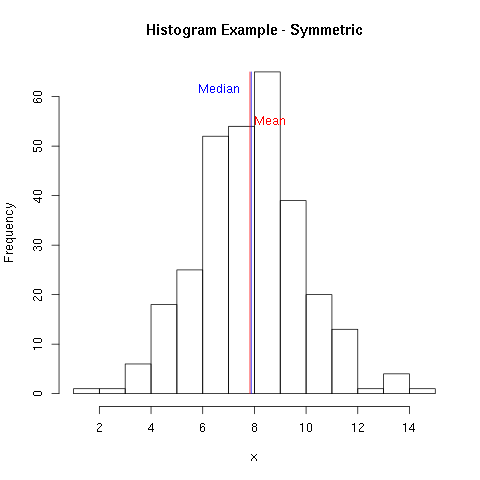
\includegraphics[width=7cm]{img/symmetricAnnotated}
  }

  
\end{frame}



\iftoggle{clicker}{%
  \begin{frame}
    \frametitle{Clicker Quiz}
    (Use channel 42)

    Find the standard deviation of the following data set:
    \vfill 

    \begin{tabular}{llll}
      3, & 3, & 2, & 4
    \end{tabular}

    \vfill

    \begin{tabular}{l@{\hspace{3em}}l@{\hspace{3em}}l@{\hspace{3em}}l}
      a: 0.5  & b: 0.667  & C: 0.707 & D: 0.816
    \end{tabular}

    \vfill

  

  \end{frame}
}







% LocalWords:  Clarkson pausesection hideallsubsections


\lecture{Grouped Data}{grouped-data}
\section{Grouped Data}


\title{Grouped Data}
\subtitle{Working with Grouped Data}

%\author{Kelly Black}
%\institute{Clarkson University}
\date{23 October 2013}

\begin{frame}
  \titlepage
\end{frame}

\begin{frame}
  \frametitle{Outline}
  \tableofcontents[hideothersubsections,sectionstyle=show/hide]
\end{frame}


\iftoggle{clicker}{%
  \subsection{Clicker Quiz}


  \begin{frame}
    \frametitle{Clicker Quiz}

    \vfill
    Find the median of the following data set:\\
    \begin{tabular}{llllll}
      28, & 17, & 12, & 20, & 21, & 18
    \end{tabular}

    \vfill
    
    \begin{tabular}{l@{\hspace{3em}}l@{\hspace{3em}}ll@{\hspace{3em}}l}
      A: 17 & B: 18 & C: 19 & D: 20
    \end{tabular}

    \vfill

  \end{frame}

}



\subsection{Sample Mean}

\begin{frame}{Sample Mean}

  We run an experiment and get data: \\
    \begin{tabular}{l|l}
      Number  & Value \\ \hline
      1 & $x_1$ \\
      2 & $x_2$ \\
      3 & $x_3$ \\
      $\vdots$ & $\vdots$ \\
      $n-1$ & $x_{n-1}$ \\
      $n$ & $x_n$
    \end{tabular}

  \only<2->%
  {
    We calculate a sample mean:
    \begin{eqnarray*}
      \bar{x} & = & \frac{x_1+x_2+\cdots+x_n}{n}.
    \end{eqnarray*}
  }

  \only<3->%
  {
    Problem: If $x_1$ is a random variable then so is $\bar{x}$!
  }

  
\end{frame}


\begin{frame}{Bias}

  $X$ is a random variable with some \blueText{parameter}, $\theta$,
  associated with it. We have a \blueText{method} to estimate the
  value, $\hat{\theta}$. 

  \begin{definition}[Unbiased Estimate]
    If $E[\hat{\theta}]=\theta$ we say that $\hat{\theta}$ is an
    \blueText{unbiased} estimator.
  \end{definition}

  \begin{definition}[Biased Estimate]
    If $E[\hat{\theta}]\neq\theta$ we say that $\hat{\theta}$ is a
    \blueText{biased} estimator.
  \end{definition}
  
\end{frame}




\begin{frame}{Bias}

  \begin{definition}[bias]
    The \blueText{bias} for an estimator is defined to be
    \begin{eqnarray*}
      \mathrm{bias} & = & E[\hat{\theta}] - \theta.
    \end{eqnarray*}

  \end{definition}
  
\end{frame}


\begin{frame}{Example}

  The following estimate for the variance is biased:
  \begin{eqnarray*}
    \frac{(x_1-\bar{x})^2 + (x_2-\bar{x})^2 + \cdots + (x_n - \bar{x})^2}{n}.
  \end{eqnarray*}

  See p. 304 of the book:
  \begin{eqnarray*}
    E\left[\frac{(x_1-\bar{x})^2 + (x_2-\bar{x})^2 + \cdots + (x_n -\bar{x})^2}{n}\right] & = & 
    \sigma^2 \frac{n-1}{n}.
  \end{eqnarray*}
  
\end{frame}


\iftoggle{clicker}{%
  \subsection{Clicker Quiz}


  \begin{frame}
    \frametitle{Clicker Quiz}

    \vfill

    $X$ is a Bernoulli random variable with parameter $p$. We take $N$
    trials and count the number of successes. The count follows what
    distribution?

    \vfill
    
    \begin{tabular}{l@{\hspace{3em}}l@{\hspace{3em}}ll@{\hspace{3em}}l}
      A: Bernoulli & B: Binomial & C: Poisson
    \end{tabular}

    \vfill

  \end{frame}

}


\begin{frame}{Example}

 $X$ is a Bernoulli random variable with parameter $p$. We take $N$
 trials and count the number of successes. We then define
 \begin{eqnarray*}
   \hat{p} & = & \frac{\mathrm{count}}{N}.
 \end{eqnarray*}
 
\end{frame}





\begin{frame}{Relative Efficiency}

  \begin{definition}
    The \blueText{relative efficiency} between two estimates,
    $\hat{\theta}_1$ and $\hat{\theta}_2$ is
    \begin{eqnarray*}
      \frac{\mathrm{var}\left( \hat{\theta}_2\right) }{\mathrm{var}\left( \hat{\theta}_1\right) }
    \end{eqnarray*}
  \end{definition}
  
\end{frame}


\begin{frame}{Example}

  $X$ is normally distributed with mean $\mu$ and standard deviation
  $\sigma$. We run two experiments. In the first experiment we take 20
  observations and find a sample mean. In the second experiment we
  take 40 observations and find a sample mean. What is the relative
  efficiency between the two estimates of the mean?
  
\end{frame}


\begin{frame}{Example}

  $X$ is a Bernoulli random variable with parameter $p$. We perform an
  experiment with $N$ trials and let
  \begin{eqnarray*}
    \hat{p} & = & \frac{\mathrm{count}}{N}.
  \end{eqnarray*}

  What is the MSE?
  
\end{frame}



\lecture{Measures Of Position}{measures-of-position}
\section{Measures Of Position}


\title{More Measures Of Dispersion}
\subtitle{How Spread Out?}

%\author{Kelly Black}
%\institute{Clarkson University}
\date{17 February 2014}

\begin{frame}
  \titlepage
\end{frame}

\begin{frame}
  \frametitle{Outline}
  \tableofcontents[hideothersubsections,sectionstyle=show/hide]
\end{frame}


\iftoggle{clicker}{%
  \subsection{Clicker Quiz}


  \begin{frame}
    \frametitle{Clicker Quiz}

    \vfill
    Find the sample median of the following data set:\\
    \begin{tabular}{llllll}
      28, & 17, & 12, & 20, & 21, & 18
    \end{tabular}

    \vfill
    
    \begin{tabular}{l@{\hspace{3em}}l@{\hspace{3em}}ll@{\hspace{3em}}l}
      A: 17 & B: 18 & C: 19 & D: 20
    \end{tabular}

    \vfill

  \end{frame}

}




\subsection{Percentiles}

\begin{frame}
  \frametitle{Percentiles}

  \begin{definition}
    The P\textsuperscript{th} percentile is the data point for which P\%
    of the numbers are smaller than it.
  \end{definition}

\end{frame}

\begin{frame}
  \frametitle{Percentiles}

%  \begin{eqnarray*}
%    \begin{array}{lllll}
%      x_1 & x_2 & x_3 & \cdots & x_n \\
%    \end{array}
%  \end{eqnarray*}

  \newcount\xnum
  \newcount\xnumpos
  \only<1>
  {
    \begin{picture}(500,100)(0,0)
      \multiput(10,90)(20, 0){15}{\line(1,0){15}}
      \xnum=1
      \xnumpos=12
      \loop
      \put(\xnumpos,95){$x_{{\the\xnum}}$}
      \advance\xnumpos by 20
      \ifnum\xnum < 15 \advance\xnum by 1
      \repeat
    \end{picture}
  }

  \only<2>
  {
    \begin{picture}(310,100)(0,0)
      \multiput(10,90)(20, 0){15}{\line(1,0){15}}
      \xnum=1
      \xnumpos=12
      \loop
      \put(\xnumpos,95){$x_{{\the\xnum}}$}
      \advance\xnumpos by 20
      \ifnum\xnum < 15 \advance\xnum by 1
      \repeat
      \put(10,0){\line(0,1){80}}
      \put(310,0){\line(0,1){80}}
      \put(110,20){\vector(-1,0){100}}
      \put(210,20){\vector( 1,0){100}}
      \put(120,15){Width=n Items}
    \end{picture}
  }

  \only<3>
  {
    \begin{picture}(310,100)(0,0)
      \multiput(10,90)(20, 0){15}{\line(1,0){15}}
      \xnum=1
      \xnumpos=12
      \loop
      \put(\xnumpos,95){$x_{{\the\xnum}}$}
      \advance\xnumpos by 20
      \ifnum\xnum < 15 \advance\xnum by 1
      \repeat
      \put(10,0){\line(0,1){80}}
      \put(310,0){\line(0,1){80}}
      \put(110,20){\vector(-1,0){100}}
      \put(210,20){\vector( 1,0){100}}
      \put(120,15){Width=n Items}

      \put(250,50){\line(0,1){40}}
      \put(80,60){\vector(-1,0){70}}
      \put(180,60){\vector( 1,0){70}}
      \put(85,55){P Percent of Width}

    \end{picture}
  }

  \vfill
  
\end{frame}

\begin{frame}
  \frametitle{Percentiles}

    \begin{picture}(310,100)(0,0)
      \multiput(10,90)(20, 0){15}{\line(1,0){15}}
      \xnum=1
      \xnumpos=12
      \loop
      \put(\xnumpos,95){$x_{{\the\xnum}}$}
      \advance\xnumpos by 20
      \ifnum\xnum < 15 \advance\xnum by 1
      \repeat
      \put(10,0){\line(0,1){80}}
      \put(310,0){\line(0,1){80}}
      \put(110,20){\vector(-1,0){100}}
      \put(210,20){\vector( 1,0){100}}
      \put(120,15){Width=n Items}

      \put(250,50){\line(0,1){40}}
      \put(70,60){\vector(-1,0){60}}
      \put(190,60){\vector( 1,0){60}}
      \put(75,55){j/n items = k\textsuperscript{th} percent}

    \end{picture}


    \begin{eqnarray*}
      P & = & \frac{k}{100}, \\
      \frac{j}{n} & = & \frac{k}{100}, \\
      \Rightarrow j & = & \frac{nk}{100}.
    \end{eqnarray*}

\end{frame}

\begin{frame}
  \frametitle{Example}

  \vfill 

  Find the 85\textsuperscript{th} percentile for the following data:

  \vfill

  \only<1>
  {
    89, 85, 97 106, 94, 100, 92, 120, 92, 97, 89, 90, 103, 86, 106, 112, 100, 92, 84,
    97, 103, 91, 104, 91, 106
  }

  \only<2>
  {
    Sort it: \\
    84, 85, 86, 89, 89, 90, 91, 91, 92, 92, 92, 94, 97, 97, 97, 100,
    100, 103, 103, 104, 106, 106, 106, 112, 120
  }

  \only<3>
  {
    Sort it: \\
    84, 85, 86, 89, 89, 90, 91, 91, 92, 92, 92, 94, 97, 97, 97, 100,
    100, 103, 103, {\color{red}\underline{104}}, {\color{red}\underline{106}}, 106, 106, 112, 120
  }


  \vfill

  (There are 25 data points.)

  \vfill

\end{frame}

\begin{frame}
  \frametitle{Clicker Quiz}

  \vfill

  Find the 30\textsuperscript{th} percentile for the following data:

  185, 196, 214, 199, 199, 204


  \vfill

  \begin{tabular}{l@{\hspace{3em}}l@{\hspace{3em}}l@{\hspace{3em}}l}
    A: 185 & B: 193.8 & C: 195 & D: 196
  \end{tabular}



\end{frame}

\subsection{Box Plots}

\begin{frame}{Quartiles}

The 25\textsuperscript{th} and 75\textsuperscript{th} percentiles are
special cases called the first quartile and third quartile
respectively, \\ [12pt]
\begin{tabular}{ll}
  P\textsuperscript{25}: & {\color{red}\only<1>{First Quartile}\only<2>{$Q_1$}} \\
  P\textsuperscript{75}: & {\color{red}\only<1>{Third Quartile}\only<2>{$Q_3$}} \\
\end{tabular}
  
\end{frame}


\begin{frame}{Calculating Quartiles}

  To calculate the quartiles you can use a short cut. Divide the data
  into smaller half and larger half. Then find the sample medians of
  the two different data sets.

  \vfill

  \only<1>%
  {
    \begin{picture}(310,100)(0,0)
      \multiput(10,90)(20, 0){15}{\line(1,0){15}}
      \xnum=1
      \xnumpos=12
      \loop
      \put(\xnumpos,95){$x_{{\the\xnum}}$}
      \advance\xnumpos by 20
      \ifnum\xnum < 15 \advance\xnum by 1
      \repeat

      \put(10,0){\line(0,1){80}}
      \put(310,0){\line(0,1){80}}
      \put(85,20){\vector(-1,0){75}}
      \put(235,20){\vector( 1,0){75}}
      \put(95,15){Sample Range = difference}

    \end{picture}
  }

  \only<2>%
  {
    \begin{picture}(310,100)(0,0)
      \multiput(10,90)(20, 0){15}{\line(1,0){15}}
      \xnum=1
      \xnumpos=12
      \loop
      \put(\xnumpos,95){$x_{{\the\xnum}}$}
      \advance\xnumpos by 20
      \ifnum\xnum < 15 \advance\xnum by 1
      \repeat

      \put(10,0){\line(0,1){80}}
      \put(310,0){\line(0,1){80}}
      \put(110,20){\vector(-1,0){100}}
      \put(210,20){\vector( 1,0){100}}
      \put(120,15){Sample Range}

      \put(156,35){\line(0,1){45}}
      \put(45,40){\vector(-1,0){35}}
      \put(121,40){\vector( 1,0){35}}
      \put(50,35){Sample Median}

    \end{picture}
  }

  \only<3>%
  {
    \begin{picture}(310,100)(0,0)
      \multiput(10,90)(20, 0){15}{\line(1,0){15}}
      \xnum=1
      \xnumpos=12
      \loop
      \put(\xnumpos,95){$x_{{\the\xnum}}$}
      \advance\xnumpos by 20
      \ifnum\xnum < 15 \advance\xnum by 1
      \repeat

      \put(10,0){\line(0,1){80}}
      \put(310,0){\line(0,1){80}}
      \put(110,20){\vector(-1,0){100}}
      \put(210,20){\vector( 1,0){100}}
      \put(120,15){Sample Range}

      \put(156,35){\line(0,1){45}}
      \put(45,40){\vector(-1,0){35}}
      \put(121,40){\vector( 1,0){35}}
      \put(50,35){Sample Median}

      \put(78,50){\line(0,1){30}}
      \put(30,55){\vector(-1,0){20}}
      \put(58,55){\vector(1,0){20}}
      \put(37,50){Q1}


      \put(240,50){\line(0,1){30}}
      \put(260,55){\vector(-1,0){20}}
      \put(290,55){\vector(1,0){20}}
      \put(265,50){Q3}


    \end{picture}
  }


  \only<4>%
  {
    \begin{picture}(310,100)(0,0)
      \multiput(10,90)(20, 0){15}{\line(1,0){15}}
      \xnum=1
      \xnumpos=12
      \loop
      \put(\xnumpos,95){{\color{red}$x_{{\the\xnum}}$}}
      \advance\xnumpos by 20
      \ifnum\xnum < 3 \advance\xnum by 1
      \repeat

      \xnum=5
      \xnumpos=92
      \loop
      \put(\xnumpos,95){{\color{blue}$x_{{\the\xnum}}$}}
      \advance\xnumpos by 20
      \ifnum\xnum < 7 \advance\xnum by 1
      \repeat

      \xnum=9
      \xnumpos=172
      \loop
      \put(\xnumpos,95){{\color{Violet}$x_{{\the\xnum}}$}}
      \advance\xnumpos by 20
      \ifnum\xnum < 12 \advance\xnum by 1
      \repeat

      \xnum=13
      \xnumpos=252
      \loop
      \put(\xnumpos,95){{\color{Brown}$x_{{\the\xnum}}$}}
      \advance\xnumpos by 20
      \ifnum\xnum < 15 \advance\xnum by 1
      \repeat


      \put(72,95){$x_{4}$}
      \put(152,95){$x_{8}$}
      \put(232,95){$x_{12}$}

      \put(10,0){\line(0,1){80}}
      \put(310,0){\line(0,1){80}}
      \put(110,20){\vector(-1,0){100}}
      \put(210,20){\vector( 1,0){100}}
      \put(120,15){Sample Range}

      \put(156,35){\line(0,1){45}}
      \put(45,40){\vector(-1,0){35}}
      \put(121,40){\vector( 1,0){35}}
      \put(50,35){Sample Median}

      \put(78,50){\line(0,1){30}}
      \put(30,55){\vector(-1,0){20}}
      \put(58,55){\vector(1,0){20}}
      \put(37,50){Q1}

      \put(240,50){\line(0,1){30}}
      \put(260,55){\vector(-1,0){20}}
      \put(290,55){\vector(1,0){20}}
      \put(265,50){Q3}

    \end{picture}
  }


  \vfill
  
\end{frame}

\begin{frame}{Example}

  Find the minimum, first quartile, sample median, third quartile, and
  maximum of the data:\\
  \begin{tabular}{lllllllll}
    40 & 21 & 38 & 38 & 27 & 36 & 34 & 33 & 26
  \end{tabular}

  \only<2->%
  {
    \vfill
    Sort the data: \\
    \begin{tabular}{lllllllll}
      21 & 26 & 27 & 33 & 34 & 36 & 38 & 38 & 40
    \end{tabular}
  }

  \vfill
  
\end{frame}


\begin{frame}{Five Point Summary}

  \begin{definition}[Five Point Summary]

    The five point summary for a data set is the minimum, first
    quartile, sample median, third quartile, and maximum of the data.
    
  \end{definition}

  \begin{definition}[Inter-Quartile Range]

    The Inter-Quartile Range (IQR) is defined to be Q3-Q1.
    
  \end{definition}




  \only<2->%
  {
    The five point summary for the data \
    \begin{tabular}{lllllllll}
      21 & 26 & 27 & 33 & 34 & 36 & 38 & 38 & 40
    \end{tabular}
    is \\
    \begin{tabular}{lllll}
      Min & Q1   & Median & Q3 & Max \\
      21  & 26.5 & 34     & 38 & 40
    \end{tabular}

    The IQR is 38-26.5=11.5.
  }

  
\end{frame}


\begin{frame}
  \frametitle{Box Plots}

  \vfill 

  Find the five point summary for the following data:

  \vfill

  \only<1>
  {
    89, 85, 97, 106, 94, 100, 92, 120, 92, 97, 89, 90, 103, 86, 106, 112, 100, 92, 84,
    97, 103, 91, 104, 91, 106

    \vfill
  }

  \only<2>
  {
    Sort it: \\
    84, 85, 86, 89, 89, 90, 91, 91, 92, 92, 92, 94, 97, 97, 97, 100,
    100, 103, 103, 104, 106, 106, 106, 112, 120

    Five point summary: \\
    \begin{tabular}{lllll}
     Min. & 1st Qu. & Median    & 3rd Qu. &   Max. \\
     84   & 91      & 97        & 103     & 120
    \end{tabular}


  }

  \vfill

\end{frame}


\begin{frame}
  \frametitle{Box Plots}

    Five point summary: \\
    \begin{tabular}{lllll}
     Min. & 1st Qu. & Median    & 3rd Qu. &   Max. \\
     84   & 91      & 97        & 103     & 120
    \end{tabular}

    \begin{center}
      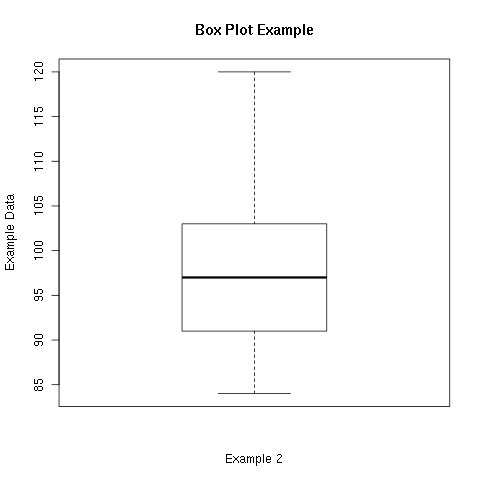
\includegraphics[width=6cm]{img/boxplotExample1}
    \end{center}

\end{frame}


\begin{frame}{Outliers}

  \begin{definition}[Outliers]

    If a number in a data set is less than Q1-$\frac{3}{2}$IQR it is
    an outlier.

    ~ \\

    If a number in a data set is more than Q3+$\frac{3}{2}$IQR it is
    an outlier.

  \end{definition}
  
\end{frame}

\begin{frame}{Example}

  \begin{tabular}{lllllllll}
    40 & 21 & 38 & 38 & 27 & 36 & 34 & 33 & 53 
  \end{tabular}

  \only<2->%
  {
    Sort the data: \\
    \begin{tabular}{lllllllll}
      21 & 27 & 33 & 34 & 36 & 38 & 38 & 40 & 53
    \end{tabular}

    \vfill

    Five point summary: \\
    \begin{tabular}{lllll}
      Min. & 1st Qu. & Median    & 3rd Qu. &   Max. \\
      21   & 30      & 36        & 39     & 53
    \end{tabular}

    \vfill
    
    \uncover<3->{
      {\color{red}The IQR is 39-30=9.}
    }

    \uncover<4->{
      ~ \\
      {\color{blue}Anything smaller than $30-\frac{3}{2}9=16.5$ is an outlier.}
    }

    \uncover<5->{
      ~ \\
      {\color{green}Anything greater than $39+\frac{3}{2}9=52.5$ is an outlier.}
    }

  }
  
\end{frame}


\begin{frame}
  \frametitle{Z-Score}

  You sample a random variable with mean $\mu$ and standard deviation
  $\sigma$.

  \begin{definition}[Z-Score]
    Given a set of data,
    \begin{eqnarray*}
      x_1,~x_2,~x_3,\ldots,x_n,
    \end{eqnarray*}
    from a random variable with mean $\mu$ and standard deviation
    $\sigma$ the $z$-score for a number, $x_i$, is
    \begin{eqnarray*}
      z_i & = & \frac{x_i-\mu}{\sigma}.
    \end{eqnarray*}
  \end{definition}

\end{frame}


% LocalWords:  Clarkson pausesection hideallsubsections hideothersubsections
% LocalWords:  sectionstyle IQR


\lecture{Assessing Normality}{assessing-normality}
\section{Assessing Normality}

\title{Assessing Normality}
\subtitle{What is the Distribution?}

%\author{Kelly Black}
%\institute{Clarkson University}
\date{19 Feb 2014}

\begin{frame}
  \titlepage
\end{frame}

\begin{frame}
  \frametitle{Outline}
  \tableofcontents[hideothersubsections,sectionstyle=show/hide]
\end{frame}


\iftoggle{clicker}{%
  \subsection{Clicker Quiz}


  \begin{frame}
    \frametitle{Clicker Quiz}

    Determine the first quartile (Q1) for the following data: \\
    \begin{tabular}{llllll}
      17 & 16 & 18 & 18 & 13 & 15 
    \end{tabular}
 
    \vfill

    \begin{tabular}{l@{\hspace{3em}}l@{\hspace{3em}}l}
      A:  15 & B: 16 & C: 16.5
    \end{tabular}

    \vfill
    \vfill
    \vfill

  \end{frame}
}




\subsection{Assessing Normality}

\begin{frame}
  \frametitle{Given Data Is It Normally Distributed?}

  Given a set of data you want to know if it is consistent with some
  distribution. Here we focus on the normal distribution. 

  The Idea - \textbf{If the random variable is normally distributed then}
  \begin{itemize}
  \item You can calculate a $z$-statistic for each number in the data
    set.
  \item The percentile of each $z$-statistic should be consistent with
    the corresponding percentile within the data.
  \item If you plot the actual $z$-statistic as a function of the
    theoretical $z$-statistic of the data point's percentile it should
    give a straight line.
  \end{itemize}
  
\end{frame}

\begin{frame}
  \frametitle{Normal Probability Plot}

  Given a data set,
  \begin{eqnarray*}
    y_1,~y_2,~y_3,\ldots,y_n,
  \end{eqnarray*}
  we construct a normal probability plot to provide an initial
  estimate how closely the data conforms to a normal distribution.

  \begin{enumerate}
    \only<1>{\item Sort the data from low to high,
      \begin{eqnarray*}
        x_1,~x_2,~x_3,\ldots,x_n, \\
        x_i & \leq & x_{i+1}.
      \end{eqnarray*}}
  \only<1>{\item Calculate the sample mean,
    \begin{eqnarray*}
      \bar{x} & = & \frac{x_1+x_2+\cdots+x_n}{n}.
    \end{eqnarray*}}
  \only<1>{\item Calculate the sample standard deviation,
    \begin{eqnarray*}
      s^2 & = & \frac{(x_1-\bar{x})^2 + \cdots + (x_n-\bar{x})^2}{n-1}, \\
      s & = & \sqrt{s^2}.
    \end{eqnarray*}}
  \only<2>{\item For each data point compute its percentile within the data
    assuming a normal distribution,
    \begin{eqnarray*}
      f_i & = & \frac{i-\frac{3}{8}}{n+\frac{1}{4}}.
    \end{eqnarray*}}
  \only<2>{\item Calculate the $z$-statistic associated with $f_i$ by working
    the standard normal table backwards to get $Z^*_i$.}
  \only<2>{\item Calculate the $z$-statistic associated with $x_i$ using
    \begin{eqnarray*}
      z_i & = & \frac{x_i-\bar{x}}{s}.
    \end{eqnarray*}}
  \only<2>{\item Plot each data pair, $(z_i,Z^*_i)$, on a plot. }
  \end{enumerate}
  
\end{frame}

\begin{frame}
  \frametitle{Example}

  First, nobody does this by hand. {\color{red}This is something that
    is done on a computer.}  \uncover<2->{{\color{blue}You still need to know how
    to interpret these graphs!}}

  \uncover<3->{%
    \begin{columns}

      \column{.4\textwidth}
      Given the data, \\
      \begin{tabular}{llllll}
        17 & 16 & 18 & 18 & 13 & 15
      \end{tabular} \\
      The normal probability plot is shown.

      \column{.5\textwidth}

      \includegraphics[width=5cm]{img/normalQQEx1}

    \end{columns}
  }
  
  
\end{frame}

\begin{frame}
  \frametitle{Example}


  \begin{columns}

    \column{.4\textwidth}
    Given the data, \\
    \begin{tabular}{llllll}
      9 & 12 & 11 & 8 & 10 & 12
    \end{tabular} \\
    The normal probability plot is shown.

  \column{.5\textwidth}

  \includegraphics[width=5cm]{img/normalQQEx2}

  \end{columns}
  
  
\end{frame}


%%% Local Variables: 
%%% mode: latex
%%% TeX-master: "IntroStats"
%%% End: 


\lecture{Normal Approximation of the Binomial}{normal-approximation-to-binomial}
\section{Normal Approximation of the Binomial}

\title{Normal Approximation of the Binomial}
\subtitle{Making the Binomial Distribution Tractable}

%\author{Kelly Black}
%\institute{Clarkson University}
\date{22 February 2013}

\begin{frame}
  \titlepage
\end{frame}

\begin{frame}
  \frametitle{Outline}
  \tableofcontents[pausesection,hideothersubsections,sectionstyle=show/hide]
\end{frame}


\iftoggle{clicker}{%
  \subsection{Clicker Quiz}


  \begin{frame}
    \frametitle{Clicker Quiz}

    Determine the value of $a$ that satisfies
    \begin{eqnarray*}
      p(z \leq a) & = & 0.95.
    \end{eqnarray*}

    \vfill

    \begin{tabular}{l@{\hspace{3em}}l@{\hspace{3em}}l}
      A: .8289 & B: 1.565 & C: 1.645
    \end{tabular}

    \vfill
    \vfill
    \vfill


  \end{frame}
}




\subsection{Normal Distribution}

\begin{frame}
  \frametitle{Example}

  A random variable, $X$, is normally distributed with mean 2.5 and a
  standard deviation of 3.6. Find $a$ so that
  \begin{eqnarray*}
    p(-2.0 \leq X \leq a) & = & 0.80.
  \end{eqnarray*}

\end{frame}

\subsection{Binomial Approximation}

\begin{frame}

  \begin{block}{Binomial Approximation}
    Suppose that $X$ is a random variable that follows a binomial
    distribution. It has $N$ repetitions, and the probability of a
    success is $p$. 

    \textbf{IF} $N\cdot p\geq 5$ \textbf{AND} $N\cdot (1-p) \geq 5$
    then $X$ can be approximated using a normal distribution:

    \begin{center}
      \begin{tabular}{ll}
        Mean: & $N\cdot p$, \\
        Std. Dev. & $\sqrt{N\cdot p \cdot (1-p)}$,
      \end{tabular}
    \end{center}

    and

    \begin{eqnarray*}
      p(X \leq a) & \approx &
       p\lp Z \leq \frac{a+0.5-N\cdot p}{\sqrt{N\cdot p \cdot (1-p)}}\rp.
    \end{eqnarray*}

  \end{block}

\end{frame}

\begin{frame}{Binomial Distribution}

  \only<1>{\includegraphics[width=6cm]{img/binomialN40}}
  \only<2>{\includegraphics[width=6cm]{img/binomialApproximationN40}}
  
\end{frame}

\subsection{Examples}

\begin{frame}{Example}
  You want to take a poll of eighty employees. You will ask them if
  they like their benefits package. You suspect that 35\% of all
  employees do like their benefits. What is the probability that
  twenty-two or less will say they do?
\end{frame}


\begin{frame}{Example}
  You want to take a poll of eighty employees. You will ask them if
  they like their benefits package. You suspect that 35\% of all
  employees do like their benefits. Determine the cut-off where there
  is a twenty-five percent chance that fewer than the cut-off will say
  they do like their benefits.
\end{frame}


\iftoggle{clicker}{%
  \begin{frame}{Clicker Quiz}
    Clarkson University claims that over eighty percent of all students
    take part in intramural sports. You choose three hundred students at
    random. What is the probability that more than two-hundred and fifty will say
    that they take part in intramural sports?

    \vfill

    \begin{tabular}{l@{\hspace{3em}}l@{\hspace{3em}}l}
      A: 0.0643  & B: 0.4679 & C: 0.9375
    \end{tabular}

    \vfill
    \vfill
    \vfill

  \end{frame}
}



% LocalWords:  Clarkson pausesection hideallsubsections

% %%%%%%%%%%%%%%%%%%%%%%%%%%%%%%%%%%%%%%%%%%%%%%%%%%%%%%%%%%%%

\lecture{More Sample Distributions}{more-sample-distributions}
\section{More Sample Distributions}

\title{More Sample Distributions}
\subtitle{More Examples}

%\author{Kelly Black}
%\institute{Clarkson University}
\date{Feb 27, 2013}

\begin{frame}
  \titlepage
\end{frame}

\begin{frame}
  \frametitle{Outline}
  \tableofcontents[pausesection,hideothersubsections,sectionstyle=show/hide]
\end{frame}


\subsection{Clicker Quiz}


\iftoggle{clicker}{%
  \begin{frame}
    \frametitle{Clicker Quiz}

    The mass of the contents of a product are normally distributed
    with a mean of 0.35 kg and a standard deviation of 0.04 kg. What
    is the probability that one sample will be less than 0.33 kg?

    \vfill

    \begin{tabular}{l@{\hspace{3em}}l@{\hspace{3em}}l@{\hspace{3em}}l}
      A: .31  & B: 0.34  & C: 0.50 & D: 0.69
    \end{tabular}

    \vfill
    \vfill
    \vfill

  \end{frame}
}


\subsection{The Sample Mean}

\iftoggle{clicker}{%
  \begin{frame}{Flip a Coin}

    Everybody: Flip a coin three times. Count the number of
    Heads. Press the number associated with the count on your clicker.

    \only<2->%
    {
      Do it again.
    }
  
  \end{frame}
}

\begin{frame}{Coin Flip}

What did we just do? 

  \only<2->%
  {
    We just calculated a sample mean. Twice!
  }

  \only<3->%
  {
    Each time we run these experiments we can get different results.

    The sample mean is a random variable.
  }
  
\end{frame}

\subsection{The Sample Mean}

\begin{frame}
  \frametitle{Sample Mean}

  We have a bunch of measurements:
  \begin{eqnarray*}
    \bar{x} & = & x_1,~x_2,~x_3,\cdots,~x_n.
  \end{eqnarray*}
  Each measurement has a mean, $\mu$, and a standard deviation of
  $\sigma$. We assume that they are all independent of one another.
  
  \only<1-2>
  {
    \begin{definition}
      Given measurements the sample mean is 
      \begin{eqnarray*}
        \bar{x} & = & \frac{x_1+x_2+x_3+\cdots+x_n}{n}.
      \end{eqnarray*}
    \end{definition}
  }

  \only<3->
  {
    \begin{definition}
      Given measurements the sample mean is 
      \begin{eqnarray*}
        \bar{x} & = & \frac{x_1+x_2+x_3+\cdots+x_n}{n}.
      \end{eqnarray*}
      The sample mean, $\bar{x}$,  has a mean of $\mu$, and it has a
      standard deviation of $\frac{\sigma}{\sqrt{n}}$.
    \end{definition}
  }


  \only<2->
  {
    The sample mean is a random variable!
  }

\end{frame}


\begin{frame}
  (central limit theorem example)
\end{frame}


\begin{frame}
  \frametitle{Distribution of the Sample Mean}

  We have a random variable, $X$, which has mean $\mu$ and standard
  deviation $\sigma.$

  We have a collection of measurements:
  \begin{eqnarray*}
    \bar{x} & = & x_1,~x_2,~x_3,\cdots,~x_n.
  \end{eqnarray*}
  Each measurement has a mean, $\mu$, and a standard deviation of
  $\sigma$. We assume that they are all independent of one another.
  
  Given the measurements the sample mean is
  \begin{eqnarray*}
    \bar{x} & = & \frac{x_1+x_2+x_3+\cdots+x_n}{n}.
  \end{eqnarray*}
  The sample mean, $\bar{x}$,  has a mean of $\mu$, and it has a
  standard deviation of $\frac{\sigma}{\sqrt{n}}$.

\end{frame}



\subsection{Examples}

\begin{frame}
  \frametitle{Example}

  The life time of batteries is normally distributed with a mean of
  19.8 hours and a standard deviation of 1.3 hours. What is the
  probability that a sample size of six batteries will give a sample
  mean that is more than 21.1 hours?

\end{frame}


\begin{frame}
  \frametitle{Example}

  You want to estimate the start up costs for restaurants in an
  area. If the mean start up costs are \$235,000 with a standard
  deviation of \$45,000 what is the probability that a sample of
  twenty restaurants will be between \$260,000 and \$205,000?

\end{frame}


\begin{frame}
  \frametitle{Example}

  You want to estimate the start up costs for restaurants in an
  area. If the mean start up costs are \$235,000 with a standard
  deviation of \$45,000 how many restaurants should you poll so that
  the probability to be within \$1,000 of the mean is eighty percent?

\end{frame}


\iftoggle{clicker}{%
  \begin{frame}
    \frametitle{Clicker Quiz}

    You want to estimate the start up costs for restaurants in an
    area. The mean start up costs are \$235,000 with a standard
    deviation of \$45,000. What is the probability that twenty samples
    will give a sample mean greater than \$245,000?


    \vfill

    \begin{tabular}{l@{\hspace{3em}}l@{\hspace{3em}}l@{\hspace{3em}}l}
      A: 0.1611  & B: 0.4021  & C: 0.4121 & D: 0.9999
    \end{tabular}

    \vfill
    \vfill
    \vfill

  \end{frame}
}



% LocalWords:  Clarkson pausesection hideallsubsections hideothersubsections
% LocalWords:  sectionstyle


\lecture{Sample Proportions}{sample-proportions}
\section{Sample Proportions}

\title{Sample Proportions}
\subtitle{Sampling a Binomial Distribution}

%\author{Kelly Black}
%\institute{Clarkson University}
\date{26 February 2014}

\begin{frame}
  \titlepage
\end{frame}

\begin{frame}
  \frametitle{Outline}
  \tableofcontents[hideothersubsections,sectionstyle=show/hide]
\end{frame}



\subsection{Clicker Quiz}


\iftoggle{clicker}{%
  \begin{frame}{Clicker Quiz}

    \iftoggle{clicker}{%

      It is estimated that 51\% of the people in a congressional
      district support the incumbent.  A poll is conducted in which 1000
      people are called and asked if they support the incumbent. The
      total number of people who say ``yes'' is counted. What is the
      distribution that the total will follow?

      \vfill 


      \begin{tabular}{l@{\hspace{3em}}l@{\hspace{3em}}l@{\hspace{3em}}l}
        A: Binomial  & B: Normal & C: Poisson
      \end{tabular}

      \vfill
      \vfill
      \vfill

    }

  \end{frame}
}





\subsection{Sample Proportions}

\begin{frame}
  \frametitle{Clicker Example}

  Will Snooki's love child be a boy or a girl?

  \begin{tabular}{l@{\hspace{3em}}l}
    A: Boy    & B: Girl
  \end{tabular}
  
  

  \vfill

  \only<2->{ 

    Left section: Will Snooki's love child be a boy or a
    girl?

    \begin{tabular}{l@{\hspace{3em}}l@{\hspace{3em}}l}
      A: Boy   & B: Girl & C: Not in left section
    \end{tabular}

  }

  \vfill

  \only<3->{ 

    Center section: Will Snooki's love child be a boy or a
    girl?

    \begin{tabular}{l@{\hspace{3em}}l@{\hspace{3em}}l}
      A: Boy   & B: Girl& C: Not in center section
    \end{tabular}

  }

  \vfill

  \only<4->{ 

    Right section: Will Snooki's love child be a boy or a
    girl?

    \begin{tabular}{l@{\hspace{3em}}l@{\hspace{3em}}l}
      A: Boy    & B: Girl & C: Not in right section
    \end{tabular}

  }

  \vfill


\end{frame}


\begin{frame}
  \frametitle{Clicker Example}

  \begin{itemize}
  \item We just made samples. (This is a not a random sample, but you
    get the idea.)

  \item Each time you take a sample you \textit{could} get something
    different.

  \item We make a calculation based on the sample. The calculation is
    called the ``sample proportion.''

    \only<2->{%
      \begin{definition}[The Sample Proportion]
        The sample proportion is defined to be
        \begin{eqnarray*}
          \hat{p} & = & \frac{\mathrm{Number~of~Yeses}}{\mathrm{Total~Number}}.
        \end{eqnarray*}
      \end{definition}

    }

  \end{itemize}

  \vfill


\end{frame}

\begin{frame}{Sampling a Binomial Distribution}

  Recall that if $X$ be a binomial distribution with a probability $p$
  of success and $n$ trials.
  \begin{itemize}
  \item Check if $n\cdot p \geq 5$ 
  \item Check if $n\cdot (1-p) \geq 5$ 
  \item If \textbf{both} conditions are true then $X$ is approximately
    normally distributed with mean $n\cdot p$ and standard deviation
    $\sqrt{p(1-p)n}$.
  \end{itemize}

  
\end{frame}


\begin{frame}
  \frametitle{Not What We Have!}

  We are not seeking the number ``yeses.''
  Instead we are asked about the \textit{proportion} of ``yeses.''

  \vfill

  \begin{definition}[The sample proportion]

    We take a sample from $n$ trials. Each trial has probability $p$
    of ``success.'' We count the total number of successes from the
    $n$ trials.  The sample proportion is defined to be
    \begin{eqnarray*}
      \hat{p} & = & \frac{\mathrm{number~of~successes}}{n}.
    \end{eqnarray*}
    
  \end{definition}



\end{frame}

\begin{frame}
  \frametitle{The sample proportion}

  The sample proportion has a mean of $p$, and a standard deviation of
  $\sqrt{\frac{p(1-p)}{n}}$.

  \vfill

  \only<2->
  {

    If $p\cdot n \geq 5$ \textbf{and} $(1-p)\cdot n \geq 5$
    \textbf{and} $n\geq 20$ then $\hat{p}$ is approximately normally
    distributed with mean $p$ and standard deviation
    $\sqrt{\frac{p(1-p)}{n}}$.

  }

  \vfill

  \only<3->
  {
    If this is the case we have
    \begin{eqnarray*}
      z & = & \frac{\hat{p}-p}{\sqrt{\frac{p(1-p)}{n}}}.
    \end{eqnarray*}
  }

  \vfill

  \only<4->
  {

    Problem: We usually do not know $p$. {\color{red}If necessary use
      the largest possible value of the standard deviation as a
      ``worst case scenario.''} That occurs when $p=\frac{1}{2}$, and
    we sometimes use that if we are not sure.

  }


\end{frame}


\subsection{Examples}

\begin{frame}
  \frametitle{Example}

  Roughly 51\% of the people in a district support the
  incumbent. One-thousand people are polled. What is the probability
  that less than half of the people will say ``yes?''

  \vfill


\end{frame}

\begin{frame}{Example}

  It is estimated that 64\% of the people who get a flu shot this year
  will not get the flu. Four hundred people who have had the shot are
  polled. What is the probability that less than 34\% of them will get
  the flu?

    \vfill

\end{frame}



\iftoggle{clicker}{%
  \begin{frame}{Clicker Quiz}


    A previous study indicates that 34\% of people who use a cell
    phone regularly will get parotid gland cancer. Two hundred people
    are tracked who are regular cell phone users. What is the
    probability that fewer than 30\% of the people will get parotid
    gland cancer?

    \vfill 


    \begin{tabular}{l@{\hspace{3em}}l@{\hspace{3em}}l@{\hspace{3em}}l}
      A: 0.10  & B: 0.11 & C: 0.12 & D: 0.13
    \end{tabular}

    \vfill
    \vfill
    \vfill



\end{frame}

}



\begin{frame}{In a nutshell}


  You conduct $n$ trials. Each trial has a probability $p$ for
  ``success'' and a probability of $1-p$ for a different
  result. Define the sample proportion to be 
  \begin{eqnarray*}
    \hat{p} & = & \frac{\mathrm{number~of~successes}}{\mathrm{number~of~trials}}.
  \end{eqnarray*}

  \begin{itemize}
  \item The sample proportion has a mean of $p$, and a standard
    deviation of $\sqrt{\frac{p(1-p)}{n}}$.
  \item Check to see if $p\cdot n \geq 5$, $(1-p)\cdot n \geq 5$ and
    $n\geq 20$. If \textit{all} of these things are true then a
    $z$-statistic can be approximated using
    \begin{eqnarray*}
      z & = & \frac{\hat{p}-p}{\sqrt{\frac{p(1-p)}{n}}}.
    \end{eqnarray*}


  \end{itemize}



  
\end{frame}

\begin{frame}{Example}

  I want to conduct a poll. It is estimated that each time I ask
  someone the question there is a probability of 0.35 that the person
  will say ``yes.'' How many people should I poll so that there is a
  probability of 0.05 that the sample proportion will be less than
  0.30?

  \vfill


\end{frame}

\begin{frame}{Example}

  I want to conduct a poll, and each question will be answered with
  either a ``yes'' or a ``no.''  How many people should I poll so that
  there is a probability of 0.05 that the sample proportion will be
  less than 0.1 lower than the true value?

  \vfill


\end{frame}



% LocalWords:  Clarkson pausesection hideallsubsections hideothersubsections
% LocalWords:  sectionstyle Kanye parotid

% %%%%%%%%%%%%%%%%%%%%%%%%%%%%%%%%%%%%%%%%%%%%%%%%%%%%%%%%%%%%

\lecture{Confidence Intervals}{confidence-interval}
\section{Confidence Intervals}

\title{The Confidence Interval}
\subtitle{Introducing the Idea}

%\author{Kelly Black}
%\institute{Clarkson University}
\date{28 February 2014}

\begin{frame}
  \titlepage
\end{frame}

\begin{frame}
  \frametitle{Outline}
  \tableofcontents[hideothersubsections,sectionstyle=show/hide]
\end{frame}


\subsection{Clicker Quiz}

\iftoggle{clicker}{%
  \begin{frame}
    \frametitle{Clicker Quiz}

    You sample a random variable which has a mean of 2.1 and a standard
    deviation of 4.5. You take 30 samples. What is the probability that
    the sample mean is more than 3.5?

    \vfill

    \begin{tabular}{l@{\hspace{3em}}l@{\hspace{3em}}l@{\hspace{3em}}l}
      A: 0.0446  & B: 0.6221  & C: 0.9954
    \end{tabular}

    \vfill
    \vfill
    \vfill

  \end{frame}
}

\subsection{The Confidence Interval}


\begin{frame}
  \frametitle{Problem!}

  We have a random variable, $X$. We want to know what its mean,
  $\mu$, or its standard deviation, $\sigma$, is. How do we figure
  this out?

  \vfill

  \only<2->
  {
    \begin{block}{Example}
      We run a capitol investment firm. Someone says that they need
      \$250,000 to start a restaurant. It this a reasonable amount?
    \end{block}
  }

  \vfill

\end{frame}


\begin{frame}{The Big Question}

  How do we estimate the mean of a random variable?
  
\end{frame}


\begin{frame}{Example}
  
  We call up ten random restaurant owners and ask them for the amount
  they needed to get started. We get the following amounts:
  \begin{tabular}{lllll}
    \$250,397 & \$241,621 & \$238,706 & \$249,276 & \$248,577 \\
    \$260,748 & \$268,647 & \$269,197 & \$232,603 & \$221,389
  \end{tabular}

  We then calculate a \textit{sample mean},
  \begin{eqnarray*}
    \bar{x} & = &
    \frac{250397+241621+238706+\cdots+232603+221389}{10}, \\
    & = & \$248,116.10\\
  \end{eqnarray*}
  This is our \textbf{estimate} for the mean.
  
\end{frame}


\iftoggle{clicker}{%
  \begin{frame}
    \frametitle{Clicker Quiz}

    We call up ten random restaurant owners and ask them for the
    amount they needed to get started. We get the following amounts:
    \begin{tabular}{lllll}
    \$250,397 & \$241,621 & \$238,706 & \$249,276 & \$248,577 \\
    \$260,748 & \$268,647 & \$269,197 & \$232,603 & \$221,389
    \end{tabular}

    We then calculate a \textit{sample mean},
    \begin{eqnarray*}
      \bar{x} & = &
      \frac{250397+241621+238706+\cdots+232603+221389}{10}, \\
      & = & \$248,116.10\\
    \end{eqnarray*}

    Is this estimate close to the true mean?

    \vfill

    \begin{tabular}{l@{\hspace{3em}}l@{\hspace{3em}}l@{\hspace{3em}}l}
      A: Yes  & B: No  & C: Maybe??
    \end{tabular}

    \vfill
    \vfill
    \vfill

  \end{frame}
}

\begin{frame}{Stupid Coworker}
  
  One of your coworkers tries to suck up to the boss and also calls
  ten random restaurant owners and ask them for the amount they needed
  to get started. He got the following amounts:
  \begin{tabular}{lllll}
    \$237,031 & \$275,563 & \$255,643 & \$264,230 & \$251,355 \\
    \$257,822 & \$252,246 & \$252,851 & \$260,110 & \$247,164
  \end{tabular}

  The resulting \textit{sample mean} is
  \begin{eqnarray*}
    \bar{x} & = &
    \frac{237031+275563+255643+\cdots+260110+247164}{10}, \\
    & = & \$255,401.50\\
  \end{eqnarray*}

  \only<2->{\color{red}Which one of you is right?}
  
\end{frame}


\begin{frame}{Estimators}

  The only thing that we have is $\bar{x}$ and $s$. The problem is
  that these things are random variables.

  $\bar{x}$ is an estimate for the mean, $\mu$.

  $s$ is an estimate for the standard deviation, $\sigma$.

  \begin{definition}{Bias}
    \begin{itemize}
    \item If our estimator for a parameter is {\color{red}expected} to be less that
      the true value it has a \textit{\color{blue}negative bias.}
    \item If our estimator for a parameter is {\color{red}expected} to be more that
      the true value it has a \textit{\color{blue} positive bias.}
    \item If the {\color{red}expectation} of our estimator for a parameter is the
      same as the true value then it is \textit{\color{blue} unbiased.}
    \end{itemize}
  \end{definition}
  
  \vfill

\end{frame}

\begin{frame}{Estimator Of The Mean}

  \begin{definition}[Estimator of the mean]
    The sample mean is an estimator of the mean,
  \begin{eqnarray*}
    \bar{x} & = & \frac{x_1 + x_2 + x_3 + \cdots + x_{n}}{n}.
  \end{eqnarray*}    
  \end{definition}
  
  \vfill
  \vfill
  \vfill

\end{frame}


\begin{frame}{The Sample Mean}

\only<1>{\centerline{\includegraphics[width=6cm]{img/approximateMeanBlank}}}
\only<2>{\centerline{\includegraphics[width=6cm]{img/approximateMean}}}

Question: How close is $\bar{x}$ to $\mu$? 

Problem: We do not know what $\mu$ is!
  
\end{frame}


\begin{frame}{Confidence Interval}

  \begin{columns}
    \column{.4\textwidth}

    \centerline{\includegraphics[width=4cm]{img/confidenceInterval}}

    \column{.6\textwidth}

    In practice we usually want one of the following things:
    \begin{itemize}
    \item Determine the value of the error
    \item Determine number of samples (N)
    \item Determine the probability that we are outside of the error bounds.
    \end{itemize}

  \end{columns}
  
\end{frame}


\begin{frame}{Confidence Interval}

  \begin{columns}
    \column{.4\textwidth}
    \centerline{\includegraphics[width=4cm]{img/confidenceInterval}}

    \column{.6\textwidth}
    The key relationship:
    \begin{eqnarray*}
      p\lp \mu-\mathrm{error} \leq \bar{x} \leq \mu + \mathrm{error}\rp
      & = & 1-\alpha
    \end{eqnarray*}
    or
    \begin{eqnarray*}
      p\lp \bar{x} \leq \mu-\mathrm{error} \rp & = & \frac{\alpha}{2},
    \end{eqnarray*}
    and
    \begin{eqnarray*}
      z & = & \frac{-\mathrm{error}}{\sigma/n}.
    \end{eqnarray*}

  \end{columns}

\end{frame}



\iftoggle{clicker}{%
  \begin{frame}
    \frametitle{Clicker Quiz}


    \centerline{\includegraphics[width=6cm]{img/week8DistConfInterval}}
    If the value of $\alpha$ is increased does the length of the
    ``error'' increase or decrease?  \vfill

    \begin{tabular}{l@{\hspace{3em}}l@{\hspace{3em}}l@{\hspace{3em}}l}
      A: Increase  & B: Decrease
    \end{tabular}

    \vfill
    \vfill
    \vfill

  \end{frame}
}



\begin{frame}
  \frametitle{Estimator for the mean}


  \only<1>{\centerline{\includegraphics[width=6cm]{img/week8Dist}}}
  \only<2>{\centerline{\includegraphics[width=6cm]{img/week8DistSample}}}
  \only<3>{%
    \centerline{\includegraphics[width=6cm]{img/week8DistConfInterval}}

    We want to determine the probability that
    \begin{eqnarray*}
      \bar{x}-\mathrm{error} \leq \mu \leq \bar{x}+\mathrm{error}.
    \end{eqnarray*}

  }

\end{frame}

\begin{frame}{Confidence Interval}

  \begin{columns}
    \column{.4\textwidth}

    \centerline{\includegraphics[width=4cm]{img/confidenceInterval}}

    \column{.6\textwidth}

    We want one of the following things:
    \begin{itemize}
    \item Given $N$ and $\alpha$ calculate the error
    \item Given $N$ and the error calculate $\alpha$
    \item Given $\alpha$ and the error calculate $N$
    \end{itemize}

  \end{columns}
  
\end{frame}


\begin{frame}{The Relationship Between $N$, error, and $\alpha$}

  \only<1-2>%
  {
    We want to determine the probability that
    \begin{eqnarray*}
      \bar{x}-\mathrm{error} \leq \mu \leq \bar{x}+\mathrm{error}.
    \end{eqnarray*}
    but we can work with the relationship
    \begin{eqnarray*}
      p\lp \mu-\mathrm{error} \leq \bar{x} \leq \mu + \mathrm{error}\rp
      & = & 1-\alpha      
    \end{eqnarray*}
  }

    Focus on the error term,
    \begin{eqnarray*}
      \mu-\mathrm{error} \leq \bar{x} \leq \mu + \mathrm{error} 
    \end{eqnarray*}
    \begin{eqnarray*}
      \only<2->%
      {
        \Rightarrow
      }
      \begin{array}{rcl@{\hspace{1.5em}\mathrm{and}\hspace{1.5em}}rcl}
        \only<2->%
        {
          \mu-\mathrm{error} & \leq & \bar{x} & \bar{x} & \leq & \mu + \mathrm{error} \\
        }
        \only<3->%
        {
          \mu & \leq & \bar{x}+\mathrm{error} & \bar{x}- \mathrm{error}  & \leq & \mu  \\
          \bar{x}+\mathrm{error} & \geq & \mu  & \mu & \geq & \bar{x}- \mathrm{error} \\
        }
      \end{array}
    \end{eqnarray*}
    \only<4->%
    {
      This implies that 
      \begin{eqnarray*}
        \bar{x}-\mathrm{error} \leq  \mu \leq \bar{x} + \mathrm{error} 
      \end{eqnarray*}
    }
  
\end{frame}


\begin{frame}{Life is good}
  We want to determine the probability that
  \begin{eqnarray*}
    \bar{x}-\mathrm{error} \leq \mu \leq \bar{x}+\mathrm{error}.
  \end{eqnarray*}
  but that is the same as working with the relationship
    \begin{eqnarray*}
      p\lp \mu-\mathrm{error} \leq \bar{x} \leq \mu + \mathrm{error}\rp
      & = & 1-\alpha.
    \end{eqnarray*}

\end{frame}

\begin{frame}{Simulation}

  See the simulation.
  
\end{frame}


\begin{frame}
  \frametitle{Example}

  We contact ten restaurant owners and ask what their starting costs
  were. We get a sample mean of \$235,000 and a standard deviation of
  \$45,000. Find the 95\% confidence interval.

  \vfill

  \only<2->%
  {

    The 95\% confidence interval is from 207,109\$ to 262,891\$
    assuming a normal distribution with a sample size of ten.

  }

  \vfill

  \only<3->%
  {

    {\color{red}You must have a formal, complete sentence for your
      final answer. You should state your result and provide enough
      information to allow your reader to make an informed decision.}

  }

\end{frame}


% LocalWords:  Clarkson pausesection hideallsubsections hideothersubsections
% LocalWords:  sectionstyle


\lecture{The t-distribution}{t-table}
\section{The t-distribution}

\title{The $t$-Distribution}
\subtitle{When you only know the sample standard deviation}

%\author{Kelly Black}
%\institute{Clarkson University}
\date{28 March 2012}

\begin{frame}
  \titlepage
\end{frame}

\begin{frame}
  \frametitle{Outline}
  \tableofcontents[pausesection,hideothersubsections,sectionstyle=show/hide]
\end{frame}


\subsection{Clicker Quiz}


\begin{frame}{Clicker Quiz}

  \iftoggle{clicker}{%

    \begin{eqnarray*}
      \begin{array}{lrcl}
        H_0: & \mu & = & 350 \\
        H_a: & \mu & \neq & 350
      \end{array}
    \end{eqnarray*}

    \begin{eqnarray*}
      n & = & 13, \\
      \bar{x} & = & 412.4,\\
      s      & = & 75.0, \\
      \alpha & = & 0.01.
    \end{eqnarray*}

    \vfill 

    What is the \textit{critical} $z$-statistic?

    \begin{tabular}{l@{\hspace{3em}}l@{\hspace{3em}}l@{\hspace{3em}}l}
      A: 1.64  & B: 1.94 & C: 2.58  & D: 3.00
    \end{tabular}

    \vfill
    \vfill
    \vfill

  }

\end{frame}


\begin{frame}{Problem!}

  We do not know $\sigma$!

  What do we do?
  
\end{frame}





\subsection{The $t$-Distribution}


\begin{frame}
  \frametitle{$t$-Distribution}

  \begin{definition}[$t$-Distribution]

    A $t$-distribution is the distribution associated with the expression
    \begin{eqnarray*}
      t &  = & \frac{\bar{x}-\mu}{\lp \frac{s}{\sqrt{n}} \rp}.
    \end{eqnarray*}

    The number of ``\textit{degrees of freedom}'' is $n-1$.
    
  \end{definition}

  Because the distribution depends on $n-1$ means that we need a
  different table for every possible value of $n$. Instead we just
  have a table for the critical values for some values of $n$.
  

\end{frame}



\begin{frame}
  \frametitle{Comparison}

  \begin{columns}
    \column{0.5\textwidth}
    Normal Distribution:
    \begin{eqnarray*}
      z &  = & \frac{\bar{x}-\mu}{\lp \frac{\sigma}{\sqrt{n}} \rp}.
    \end{eqnarray*}

    \column{0.5\textwidth}
    $t$-Distribution:
    \begin{eqnarray*}
      t &  = & \frac{\bar{x}-\mu}{\lp \frac{s}{\sqrt{n}} \rp}, \\
      df & = & n-1.
    \end{eqnarray*}

  \end{columns}

  \vfill

    \only<2->
    {

      \begin{center}
        The algebra and concepts are exactly the same!

        The only difference is $\sigma$ vs. $s$ and $df=n-1$.
      \end{center}
    }

    \vfill
  

\end{frame}



\begin{frame}
  \frametitle{The Table}
  {
\fontencoding{T1}
\fontfamily{pcr}
\fontseries{m}
\fontshape{n}
\fontsize{5pt}{5pt}
\selectfont

\begin{tabular}{l|llllllllll}
 & 0.1&0.05&0.025&0.01&0.005&0.001&0.00005\\ \hline
 1 & 3.078 & 6.314 & 12.706 & 31.821 & 63.657 & 318.309 & 636.619 \\ 
 2 & 1.886 & 2.920 & 4.303 & 6.965 & 9.925 & 22.327 & 31.599 \\ 
 3 & 1.638 & 2.353 & 3.182 & 4.541 & 5.841 & 10.215 & 12.924 \\ 
 4 & 1.533 & 2.132 & 2.776 & 3.747 & 4.604 & 7.173 & 8.610 \\ 
 5 & 1.476 & 2.015 & 2.571 & 3.365 & 4.032 & 5.893 & 6.869 \\ 
[5pt]
 6 & 1.440 & 1.943 & 2.447 & 3.143 & 3.707 & 5.208 & 5.959 \\ 
 7 & 1.415 & 1.895 & 2.365 & 2.998 & 3.499 & 4.785 & 5.408 \\ 
 8 & 1.397 & 1.860 & 2.306 & 2.896 & 3.355 & 4.501 & 5.041 \\ 
 9 & 1.383 & 1.833 & 2.262 & 2.821 & 3.250 & 4.297 & 4.781 \\ 
10 & 1.372 & 1.812 & 2.228 & 2.764 & 3.169 & 4.144 & 4.587 \\ 
[5pt]
11 & 1.363 & 1.796 & 2.201 & 2.718 & 3.106 & 4.025 & 4.437 \\ 
12 & 1.356 & 1.782 & 2.179 & 2.681 & 3.055 & 3.930 & 4.318 \\ 
13 & 1.350 & 1.771 & 2.160 & 2.650 & 3.012 & 3.852 & 4.221 \\ 
14 & 1.345 & 1.761 & 2.145 & 2.624 & 2.977 & 3.787 & 4.140 \\ 
15 & 1.341 & 1.753 & 2.131 & 2.602 & 2.947 & 3.733 & 4.073 \\ 
[5pt]
16 & 1.337 & 1.746 & 2.120 & 2.583 & 2.921 & 3.686 & 4.015 \\ 
17 & 1.333 & 1.740 & 2.110 & 2.567 & 2.898 & 3.646 & 3.965 \\ 
18 & 1.330 & 1.734 & 2.101 & 2.552 & 2.878 & 3.610 & 3.922 \\ 
19 & 1.328 & 1.729 & 2.093 & 2.539 & 2.861 & 3.579 & 3.883 \\ 
20 & 1.325 & 1.725 & 2.086 & 2.528 & 2.845 & 3.552 & 3.850 \\ 
[5pt]
21 & 1.323 & 1.721 & 2.080 & 2.518 & 2.831 & 3.527 & 3.819 \\ 
22 & 1.321 & 1.717 & 2.074 & 2.508 & 2.819 & 3.505 & 3.792 \\ 
23 & 1.319 & 1.714 & 2.069 & 2.500 & 2.807 & 3.485 & 3.768 \\ 
24 & 1.318 & 1.711 & 2.064 & 2.492 & 2.797 & 3.467 & 3.745 \\ 
25 & 1.316 & 1.708 & 2.060 & 2.485 & 2.787 & 3.450 & 3.725 \\ 
[5pt]
26 & 1.315 & 1.706 & 2.056 & 2.479 & 2.779 & 3.435 & 3.707 \\ 
27 & 1.314 & 1.703 & 2.052 & 2.473 & 2.771 & 3.421 & 3.690 \\ 
28 & 1.313 & 1.701 & 2.048 & 2.467 & 2.763 & 3.408 & 3.674 \\ 
29 & 1.311 & 1.699 & 2.045 & 2.462 & 2.756 & 3.396 & 3.659 \\ 
30 & 1.310 & 1.697 & 2.042 & 2.457 & 2.750 & 3.385 & 3.646 \\ 
[5pt]
40 & 1.303 & 1.684 & 2.021 & 2.423 & 2.704 & 3.307 & 3.551 \\ 
50 & 1.299 & 1.676 & 2.009 & 2.403 & 2.678 & 3.261 & 3.496 \\ 
60 & 1.296 & 1.671 & 2.000 & 2.390 & 2.660 & 3.232 & 3.460 \\ 
120 & 1.289 & 1.658 & 1.980 & 2.358 & 2.617 & 3.160 & 3.373 \\ 
$\infty$ & 1.282 & 1.645 & 1.960 & 2.326 & 2.576 & 3.090 & 3.291 
\end{tabular}


}
\end{frame}


\begin{frame}{\small Example: Find $t^*$ value for $p(|t|>t^*)
\approx 0.01$ with 12 degrees of freedom.}
{\tiny First find the row corresponding to $n=12$.}

  {
\fontencoding{T1}
\fontfamily{pcr}
\fontseries{m}
\fontshape{n}
\fontsize{5pt}{5pt}
\selectfont

\begin{tabular}{l|llllllllll}
 & 0.1&0.05&0.025&0.01&0.005&0.001&0.00005\\ \hline
 1 & 3.078 & 6.314 & 12.706 & 31.821 & 63.657 & 318.309 & 636.619 \\ 
 2 & 1.886 & 2.920 & 4.303 & 6.965 & 9.925 & 22.327 & 31.599 \\ 
 3 & 1.638 & 2.353 & 3.182 & 4.541 & 5.841 & 10.215 & 12.924 \\ 
 4 & 1.533 & 2.132 & 2.776 & 3.747 & 4.604 & 7.173 & 8.610 \\ 
 5 & 1.476 & 2.015 & 2.571 & 3.365 & 4.032 & 5.893 & 6.869 \\ 
[5pt]
 6 & 1.440 & 1.943 & 2.447 & 3.143 & 3.707 & 5.208 & 5.959 \\ 
 7 & 1.415 & 1.895 & 2.365 & 2.998 & 3.499 & 4.785 & 5.408 \\ 
 8 & 1.397 & 1.860 & 2.306 & 2.896 & 3.355 & 4.501 & 5.041 \\ 
 9 & 1.383 & 1.833 & 2.262 & 2.821 & 3.250 & 4.297 & 4.781 \\ 
10 & 1.372 & 1.812 & 2.228 & 2.764 & 3.169 & 4.144 & 4.587 \\ 
[5pt]
11 & 1.363 & 1.796 & 2.201 & 2.718 & 3.106 & 4.025 & 4.437 \\ 
\rowcolor{red}12 & 1.356 & 1.782 & 2.179 & 2.681 & 3.055 & 3.930 & 4.318 \\ 
13 & 1.350 & 1.771 & 2.160 & 2.650 & 3.012 & 3.852 & 4.221 \\ 
14 & 1.345 & 1.761 & 2.145 & 2.624 & 2.977 & 3.787 & 4.140 \\ 
15 & 1.341 & 1.753 & 2.131 & 2.602 & 2.947 & 3.733 & 4.073 \\ 
[5pt]
16 & 1.337 & 1.746 & 2.120 & 2.583 & 2.921 & 3.686 & 4.015 \\ 
17 & 1.333 & 1.740 & 2.110 & 2.567 & 2.898 & 3.646 & 3.965 \\ 
18 & 1.330 & 1.734 & 2.101 & 2.552 & 2.878 & 3.610 & 3.922 \\ 
19 & 1.328 & 1.729 & 2.093 & 2.539 & 2.861 & 3.579 & 3.883 \\ 
20 & 1.325 & 1.725 & 2.086 & 2.528 & 2.845 & 3.552 & 3.850 \\ 
[5pt]
21 & 1.323 & 1.721 & 2.080 & 2.518 & 2.831 & 3.527 & 3.819 \\ 
22 & 1.321 & 1.717 & 2.074 & 2.508 & 2.819 & 3.505 & 3.792 \\ 
23 & 1.319 & 1.714 & 2.069 & 2.500 & 2.807 & 3.485 & 3.768 \\ 
24 & 1.318 & 1.711 & 2.064 & 2.492 & 2.797 & 3.467 & 3.745 \\ 
25 & 1.316 & 1.708 & 2.060 & 2.485 & 2.787 & 3.450 & 3.725 \\ 
[5pt]
26 & 1.315 & 1.706 & 2.056 & 2.479 & 2.779 & 3.435 & 3.707 \\ 
27 & 1.314 & 1.703 & 2.052 & 2.473 & 2.771 & 3.421 & 3.690 \\ 
28 & 1.313 & 1.701 & 2.048 & 2.467 & 2.763 & 3.408 & 3.674 \\ 
29 & 1.311 & 1.699 & 2.045 & 2.462 & 2.756 & 3.396 & 3.659 \\ 
30 & 1.310 & 1.697 & 2.042 & 2.457 & 2.750 & 3.385 & 3.646 \\ 
[5pt]
40 & 1.303 & 1.684 & 2.021 & 2.423 & 2.704 & 3.307 & 3.551 \\ 
50 & 1.299 & 1.676 & 2.009 & 2.403 & 2.678 & 3.261 & 3.496 \\ 
60 & 1.296 & 1.671 & 2.000 & 2.390 & 2.660 & 3.232 & 3.460 \\ 
120 & 1.289 & 1.658 & 1.980 & 2.358 & 2.617 & 3.160 & 3.373 \\ 
$\infty$ & 1.282 & 1.645 & 1.960 & 2.326 & 2.576 & 3.090 & 3.291 
\end{tabular}


}



\end{frame}

\begin{frame}
{\small Second find the column corresponding to 0.005. The critical $t$ value is 3.055.}

  {
\fontencoding{T1}
\fontfamily{pcr}
\fontseries{m}
\fontshape{n}
\fontsize{5pt}{5pt}
\selectfont

\begin{tabular}{l|llll>{\columncolor{blue}}llllll}
 & 0.1&0.05&0.025&0.01&0.005&0.001&0.00005\\ \hline
 1 & 3.078 & 6.314 & 12.706 & 31.821 & 63.657 & 318.309 & 636.619 \\ 
 2 & 1.886 & 2.920 & 4.303 & 6.965 & 9.925 & 22.327 & 31.599 \\ 
 3 & 1.638 & 2.353 & 3.182 & 4.541 & 5.841 & 10.215 & 12.924 \\ 
 4 & 1.533 & 2.132 & 2.776 & 3.747 & 4.604 & 7.173 & 8.610 \\ 
 5 & 1.476 & 2.015 & 2.571 & 3.365 & 4.032 & 5.893 & 6.869 \\ 
[5pt]
 6 & 1.440 & 1.943 & 2.447 & 3.143 & 3.707 & 5.208 & 5.959 \\ 
 7 & 1.415 & 1.895 & 2.365 & 2.998 & 3.499 & 4.785 & 5.408 \\ 
 8 & 1.397 & 1.860 & 2.306 & 2.896 & 3.355 & 4.501 & 5.041 \\ 
 9 & 1.383 & 1.833 & 2.262 & 2.821 & 3.250 & 4.297 & 4.781 \\ 
10 & 1.372 & 1.812 & 2.228 & 2.764 & 3.169 & 4.144 & 4.587 \\ 
[5pt]
11 & 1.363 & 1.796 & 2.201 & 2.718 & 3.106 & 4.025 & 4.437 \\ 
\rowcolor{red}12 & 1.356 & 1.782 & 2.179 & 2.681 & 3.055 & 3.930 & 4.318 \\ 
13 & 1.350 & 1.771 & 2.160 & 2.650 & 3.012 & 3.852 & 4.221 \\ 
14 & 1.345 & 1.761 & 2.145 & 2.624 & 2.977 & 3.787 & 4.140 \\ 
15 & 1.341 & 1.753 & 2.131 & 2.602 & 2.947 & 3.733 & 4.073 \\ 
[5pt]
16 & 1.337 & 1.746 & 2.120 & 2.583 & 2.921 & 3.686 & 4.015 \\ 
17 & 1.333 & 1.740 & 2.110 & 2.567 & 2.898 & 3.646 & 3.965 \\ 
18 & 1.330 & 1.734 & 2.101 & 2.552 & 2.878 & 3.610 & 3.922 \\ 
19 & 1.328 & 1.729 & 2.093 & 2.539 & 2.861 & 3.579 & 3.883 \\ 
20 & 1.325 & 1.725 & 2.086 & 2.528 & 2.845 & 3.552 & 3.850 \\ 
[5pt]
21 & 1.323 & 1.721 & 2.080 & 2.518 & 2.831 & 3.527 & 3.819 \\ 
22 & 1.321 & 1.717 & 2.074 & 2.508 & 2.819 & 3.505 & 3.792 \\ 
23 & 1.319 & 1.714 & 2.069 & 2.500 & 2.807 & 3.485 & 3.768 \\ 
24 & 1.318 & 1.711 & 2.064 & 2.492 & 2.797 & 3.467 & 3.745 \\ 
25 & 1.316 & 1.708 & 2.060 & 2.485 & 2.787 & 3.450 & 3.725 \\ 
[5pt]
26 & 1.315 & 1.706 & 2.056 & 2.479 & 2.779 & 3.435 & 3.707 \\ 
27 & 1.314 & 1.703 & 2.052 & 2.473 & 2.771 & 3.421 & 3.690 \\ 
28 & 1.313 & 1.701 & 2.048 & 2.467 & 2.763 & 3.408 & 3.674 \\ 
29 & 1.311 & 1.699 & 2.045 & 2.462 & 2.756 & 3.396 & 3.659 \\ 
30 & 1.310 & 1.697 & 2.042 & 2.457 & 2.750 & 3.385 & 3.646 \\ 
[5pt]
40 & 1.303 & 1.684 & 2.021 & 2.423 & 2.704 & 3.307 & 3.551 \\ 
50 & 1.299 & 1.676 & 2.009 & 2.403 & 2.678 & 3.261 & 3.496 \\ 
60 & 1.296 & 1.671 & 2.000 & 2.390 & 2.660 & 3.232 & 3.460 \\ 
120 & 1.289 & 1.658 & 1.980 & 2.358 & 2.617 & 3.160 & 3.373 \\ 
$\infty$ & 1.282 & 1.645 & 1.960 & 2.326 & 2.576 & 3.090 & 3.291 
\end{tabular}


}

\end{frame}


\begin{frame}{Our First Example}


    \begin{eqnarray*}
      \begin{array}{lrcl}
        H_0: & \mu & = & 350 \\
        H_a: & \mu & \neq & 350
      \end{array}
    \end{eqnarray*}

    \begin{eqnarray*}
      n & = & 13, \\
      \bar{x} & = & 412.4,\\
      s      & = & 75.0, \\
      \alpha & = & 0.01.
    \end{eqnarray*}

    \vfill 

    The \textit{critical} $t$-statistic is 
    \begin{eqnarray*}
      t^* & = & 3.055.
    \end{eqnarray*}

    The $t$-statistic from the data is
    \begin{eqnarray*}
      t & = & \frac{412.4-350}{\frac{75}{\sqrt{13}}}, \\
        & \approx & 3.00.
    \end{eqnarray*}



\end{frame}

\begin{frame}{Result}

  We \textbf{do not} have sufficient evidence to reject $H_0$ at the
  1\% significance level using a $t$-distribution with thirteen
  samples and a standard deviation of 75.
  
\end{frame}


\begin{frame}{Let's Change Our First Example}


    \begin{eqnarray*}
      \begin{array}{lrcl}
        H_0: & \mu & = & 350 \\
        H_a: & \mu & \neq & 350
      \end{array}
    \end{eqnarray*}

    \begin{eqnarray*}
      n & = & 13, \\
      \bar{x} & = & 412.4,\\
      s      & = & 75.0, \\
      \alpha & = & 0.05.
    \end{eqnarray*}

    \vfill 

    The $t$-statistic from the data is
    \begin{eqnarray*}
      t & = & \frac{412.4-350}{\frac{75}{\sqrt{13}}}, \\
        & \approx & 3.00.
    \end{eqnarray*}


    What is the critical $t$-statistic?

\end{frame}



\begin{frame}{\small Example: Find $t^*$ value for $p(|t|>t^*)
\approx 0.01$ with 12 degrees of freedom.}
  
{\small First find the row corresponding to $n=12$.}

  {
\fontencoding{T1}
\fontfamily{pcr}
\fontseries{m}
\fontshape{n}
\fontsize{5pt}{5pt}
\selectfont

\begin{tabular}{l|llllllllll}
 & 0.1&0.05&0.025&0.01&0.005&0.001&0.00005\\ \hline
 1 & 3.078 & 6.314 & 12.706 & 31.821 & 63.657 & 318.309 & 636.619 \\ 
 2 & 1.886 & 2.920 & 4.303 & 6.965 & 9.925 & 22.327 & 31.599 \\ 
 3 & 1.638 & 2.353 & 3.182 & 4.541 & 5.841 & 10.215 & 12.924 \\ 
 4 & 1.533 & 2.132 & 2.776 & 3.747 & 4.604 & 7.173 & 8.610 \\ 
 5 & 1.476 & 2.015 & 2.571 & 3.365 & 4.032 & 5.893 & 6.869 \\ 
[5pt]
 6 & 1.440 & 1.943 & 2.447 & 3.143 & 3.707 & 5.208 & 5.959 \\ 
 7 & 1.415 & 1.895 & 2.365 & 2.998 & 3.499 & 4.785 & 5.408 \\ 
 8 & 1.397 & 1.860 & 2.306 & 2.896 & 3.355 & 4.501 & 5.041 \\ 
 9 & 1.383 & 1.833 & 2.262 & 2.821 & 3.250 & 4.297 & 4.781 \\ 
10 & 1.372 & 1.812 & 2.228 & 2.764 & 3.169 & 4.144 & 4.587 \\ 
[5pt]
11 & 1.363 & 1.796 & 2.201 & 2.718 & 3.106 & 4.025 & 4.437 \\ 
\rowcolor{red}12 & 1.356 & 1.782 & 2.179 & 2.681 & 3.055 & 3.930 & 4.318 \\ 
13 & 1.350 & 1.771 & 2.160 & 2.650 & 3.012 & 3.852 & 4.221 \\ 
14 & 1.345 & 1.761 & 2.145 & 2.624 & 2.977 & 3.787 & 4.140 \\ 
15 & 1.341 & 1.753 & 2.131 & 2.602 & 2.947 & 3.733 & 4.073 \\ 
[5pt]
16 & 1.337 & 1.746 & 2.120 & 2.583 & 2.921 & 3.686 & 4.015 \\ 
17 & 1.333 & 1.740 & 2.110 & 2.567 & 2.898 & 3.646 & 3.965 \\ 
18 & 1.330 & 1.734 & 2.101 & 2.552 & 2.878 & 3.610 & 3.922 \\ 
19 & 1.328 & 1.729 & 2.093 & 2.539 & 2.861 & 3.579 & 3.883 \\ 
20 & 1.325 & 1.725 & 2.086 & 2.528 & 2.845 & 3.552 & 3.850 \\ 
[5pt]
21 & 1.323 & 1.721 & 2.080 & 2.518 & 2.831 & 3.527 & 3.819 \\ 
22 & 1.321 & 1.717 & 2.074 & 2.508 & 2.819 & 3.505 & 3.792 \\ 
23 & 1.319 & 1.714 & 2.069 & 2.500 & 2.807 & 3.485 & 3.768 \\ 
24 & 1.318 & 1.711 & 2.064 & 2.492 & 2.797 & 3.467 & 3.745 \\ 
25 & 1.316 & 1.708 & 2.060 & 2.485 & 2.787 & 3.450 & 3.725 \\ 
[5pt]
26 & 1.315 & 1.706 & 2.056 & 2.479 & 2.779 & 3.435 & 3.707 \\ 
27 & 1.314 & 1.703 & 2.052 & 2.473 & 2.771 & 3.421 & 3.690 \\ 
28 & 1.313 & 1.701 & 2.048 & 2.467 & 2.763 & 3.408 & 3.674 \\ 
29 & 1.311 & 1.699 & 2.045 & 2.462 & 2.756 & 3.396 & 3.659 \\ 
30 & 1.310 & 1.697 & 2.042 & 2.457 & 2.750 & 3.385 & 3.646 \\ 
[5pt]
40 & 1.303 & 1.684 & 2.021 & 2.423 & 2.704 & 3.307 & 3.551 \\ 
50 & 1.299 & 1.676 & 2.009 & 2.403 & 2.678 & 3.261 & 3.496 \\ 
60 & 1.296 & 1.671 & 2.000 & 2.390 & 2.660 & 3.232 & 3.460 \\ 
120 & 1.289 & 1.658 & 1.980 & 2.358 & 2.617 & 3.160 & 3.373 \\ 
$\infty$ & 1.282 & 1.645 & 1.960 & 2.326 & 2.576 & 3.090 & 3.291 
\end{tabular}


}



\end{frame}

\begin{frame}
{\small Second find the column corresponding to 0.005. The critical $t$ value is 2.179.}

  {
\fontencoding{T1}
\fontfamily{pcr}
\fontseries{m}
\fontshape{n}
\fontsize{5pt}{5pt}
\selectfont

\begin{tabular}{l|ll>{\columncolor{blue}}llllllll}
 & 0.1&0.05&0.025&0.01&0.005&0.001&0.00005\\ \hline
 1 & 3.078 & 6.314 & 12.706 & 31.821 & 63.657 & 318.309 & 636.619 \\ 
 2 & 1.886 & 2.920 & 4.303 & 6.965 & 9.925 & 22.327 & 31.599 \\ 
 3 & 1.638 & 2.353 & 3.182 & 4.541 & 5.841 & 10.215 & 12.924 \\ 
 4 & 1.533 & 2.132 & 2.776 & 3.747 & 4.604 & 7.173 & 8.610 \\ 
 5 & 1.476 & 2.015 & 2.571 & 3.365 & 4.032 & 5.893 & 6.869 \\ 
[5pt]
 6 & 1.440 & 1.943 & 2.447 & 3.143 & 3.707 & 5.208 & 5.959 \\ 
 7 & 1.415 & 1.895 & 2.365 & 2.998 & 3.499 & 4.785 & 5.408 \\ 
 8 & 1.397 & 1.860 & 2.306 & 2.896 & 3.355 & 4.501 & 5.041 \\ 
 9 & 1.383 & 1.833 & 2.262 & 2.821 & 3.250 & 4.297 & 4.781 \\ 
10 & 1.372 & 1.812 & 2.228 & 2.764 & 3.169 & 4.144 & 4.587 \\ 
[5pt]
11 & 1.363 & 1.796 & 2.201 & 2.718 & 3.106 & 4.025 & 4.437 \\ 
\rowcolor{red}12 & 1.356 & 1.782 & 2.179 & 2.681 & 3.055 & 3.930 & 4.318 \\ 
13 & 1.350 & 1.771 & 2.160 & 2.650 & 3.012 & 3.852 & 4.221 \\ 
14 & 1.345 & 1.761 & 2.145 & 2.624 & 2.977 & 3.787 & 4.140 \\ 
15 & 1.341 & 1.753 & 2.131 & 2.602 & 2.947 & 3.733 & 4.073 \\ 
[5pt]
16 & 1.337 & 1.746 & 2.120 & 2.583 & 2.921 & 3.686 & 4.015 \\ 
17 & 1.333 & 1.740 & 2.110 & 2.567 & 2.898 & 3.646 & 3.965 \\ 
18 & 1.330 & 1.734 & 2.101 & 2.552 & 2.878 & 3.610 & 3.922 \\ 
19 & 1.328 & 1.729 & 2.093 & 2.539 & 2.861 & 3.579 & 3.883 \\ 
20 & 1.325 & 1.725 & 2.086 & 2.528 & 2.845 & 3.552 & 3.850 \\ 
[5pt]
21 & 1.323 & 1.721 & 2.080 & 2.518 & 2.831 & 3.527 & 3.819 \\ 
22 & 1.321 & 1.717 & 2.074 & 2.508 & 2.819 & 3.505 & 3.792 \\ 
23 & 1.319 & 1.714 & 2.069 & 2.500 & 2.807 & 3.485 & 3.768 \\ 
24 & 1.318 & 1.711 & 2.064 & 2.492 & 2.797 & 3.467 & 3.745 \\ 
25 & 1.316 & 1.708 & 2.060 & 2.485 & 2.787 & 3.450 & 3.725 \\ 
[5pt]
26 & 1.315 & 1.706 & 2.056 & 2.479 & 2.779 & 3.435 & 3.707 \\ 
27 & 1.314 & 1.703 & 2.052 & 2.473 & 2.771 & 3.421 & 3.690 \\ 
28 & 1.313 & 1.701 & 2.048 & 2.467 & 2.763 & 3.408 & 3.674 \\ 
29 & 1.311 & 1.699 & 2.045 & 2.462 & 2.756 & 3.396 & 3.659 \\ 
30 & 1.310 & 1.697 & 2.042 & 2.457 & 2.750 & 3.385 & 3.646 \\ 
[5pt]
40 & 1.303 & 1.684 & 2.021 & 2.423 & 2.704 & 3.307 & 3.551 \\ 
50 & 1.299 & 1.676 & 2.009 & 2.403 & 2.678 & 3.261 & 3.496 \\ 
60 & 1.296 & 1.671 & 2.000 & 2.390 & 2.660 & 3.232 & 3.460 \\ 
120 & 1.289 & 1.658 & 1.980 & 2.358 & 2.617 & 3.160 & 3.373 \\ 
$\infty$ & 1.282 & 1.645 & 1.960 & 2.326 & 2.576 & 3.090 & 3.291 
\end{tabular}


}

\end{frame}



\begin{frame}{Let's Change Our First Example}


    \begin{eqnarray*}
      \begin{array}{lrcl}
        H_0: & \mu & = & 350 \\
        H_a: & \mu & \neq & 350
      \end{array}
    \end{eqnarray*}

    \begin{eqnarray*}
      n & = & 13, \\
      \bar{x} & = & 412.4,\\
      s      & = & 75.0, \\
      \alpha & = & 0.05.
    \end{eqnarray*}

    \vfill 

    The $t$-statistic from the data is
    \begin{eqnarray*}
      t & = & \frac{412.4-350}{\frac{75}{\sqrt{13}}}, \\
        & \approx & 3.00.
    \end{eqnarray*}


    \begin{eqnarray*}
      t^* & \approx & 2.179.
    \end{eqnarray*}

\end{frame}


\begin{frame}{Result}

  We have sufficient evidence to reject $H_0$ at the 5\% significance
  level using a $t$-distribution with thirteen samples and a standard
  deviation of 75.
  
\end{frame}




\begin{frame}{Clicker Quiz}

  \iftoggle{clicker}{%

    \begin{eqnarray*}
      \begin{array}{lrcl}
        H_0: & \mu & = &  10 \\
        H_a: & \mu & \neq & 10
      \end{array}
    \end{eqnarray*}

    \begin{eqnarray*}
      n & = & 17, \\
      \bar{x} & = & 8.5,\\
      s      & = & 3.0, \\
      \alpha & = & 0.05.
    \end{eqnarray*}

    \vfill 


    \begin{tabular}{l@{\hspace{3em}}l@{\hspace{3em}}l@{\hspace{3em}}l}
      A: Reject $H_0$  & B: Cannot reject $H_0$ 
    \end{tabular}

    \vfill
    \vfill
    \vfill

  }

\end{frame}





% LocalWords:  Clarkson pausesection hideallsubsections


\lecture{Confidence Intervals for the Sample Proportion}{confidence-interval-sample-proportions}
\section{Confidence Intervals for the Sample Proportion}

\title{Confidence Intervals for the Sample Proportion}
\subtitle{What percentage?}

%\author{Kelly Black}
%\institute{Clarkson University}
\date{13 March 2013}

\begin{frame}
  \titlepage
\end{frame}

\begin{frame}
  \frametitle{Outline}
  \tableofcontents[hideothersubsections,sectionstyle=show/hide]
\end{frame}


\subsection{Clicker Quiz}


\iftoggle{clicker}{%
  \begin{frame}
    \frametitle{Clicker Quiz}

    Requests are made to determine the cost of including advertisements
    on web pages.  Twenty-three responses are received, and the sample
    mean is 1,300\$ with a sample standard deviation of 320\$. What is
    the 95\% confidence interval for the mean?

    \vfill

    \begin{tabular}{l@{\hspace{3em}}l@{\hspace{3em}}l@{\hspace{3em}}l}
      A: 1169\$ to 1431\$ & B: 1190\$ to 1410\$ \\
      C: 1162\$ to 1438\$ & D: 1185\$ to 1415\$
    \end{tabular}

    \vfill
    \vfill
    \vfill

  \end{frame}
}


\subsection{Sample Proportion}

\begin{frame}{The Sample Proportion}

  You conduct $n$ trials. Each trial has a probability $p$ for
  ``success'' and a probability of $1-p$ for a different
  result. Define the sample proportion to be 
  \begin{eqnarray*}
    \hat{p} & = & \frac{\mathrm{number~of~successes}}{\mathrm{number~of~trials}}.
  \end{eqnarray*}

  \begin{itemize}
  \item The sample proportion has a mean of $p$, and a standard
    deviation of $\sqrt{\frac{p(1-p)}{n}}$.
  \item Check to see if $p\cdot n \geq 5$, $(1-p)\cdot n \geq 5$ and
    $n\geq 20$. If \textit{all} of these things are true
    \begin{itemize}
    \item $\hat{p}$ is approximately normally distributed
    \item The mean of $\hat{p}$ is mean $p$.
    \item The standard deviation of $\hat{p}$ is
      $\sqrt{\frac{p(1-p)}{n}}$
    \item A $z$-statistic can be approximated using
      \begin{eqnarray*}
        z & = & \frac{\hat{p}-p}{\sqrt{\frac{p(1-p)}{n}}}.
      \end{eqnarray*}
    \end{itemize}

  \end{itemize}



  
\end{frame}


\begin{frame}
  \frametitle{Notation}


  \begin{definition}[The Sample Proportion]

    You conduct an experiment. There are $N$ trials. The number of
    ``successes'' is $x$.  The sample proportion is defined to be 
    \begin{eqnarray*}
      \hat{p} & = & \frac{x}{N}.
    \end{eqnarray*}

    \only<2->%
    {

      If $Np\geq 5$ and $N(1-p)\geq 5$ and $N\geq 20$ then $\hat{p}$
      can be approximated by a normal distribution with mean $p$ and
      standard deviation $\sqrt{p(1-p)/N}$.

    }

    \only<3->%
    {

      Once we have the distribution then we can do all the stuff we do
      with normal distributions. (i.e. We can find confidence intervals!)

    }

  \end{definition}
  
\end{frame}

\subsection{Examples}

\begin{frame}
  \frametitle{Example}

  I conduct a poll to determine what proportion of people are
  satisfied with the company's benefits program. Forty-five people
  respond and thirty-one people say they are satisfied.  What is the
  95\% confidence interval for the proportion of people satisfied with
  their benefits?

  \only<2->%
  {

    In this case our estimate for $\hat{p}$ is 
    \begin{eqnarray*}
      \hat{p} & = & \frac{31}{45}.
    \end{eqnarray*}
    We use this as our estimate for $p$.

  }

  \only<3->%
  {

    {\color{red}
      The 95\% confidence interval is from 0.554 to 0.824 assuming a
      normal approximation with 45 samples.
    }

  }
  
\end{frame}


\begin{frame}
  \frametitle{Example}

  We want to determine how many people in a company have a commute
  that takes more than one hour one-way. One-hundred and twenty people
  respond, and forty-two say that their commute is more than one
  hour. What is the 95\% confidence interval for the proportion of
  people whose commute is more than one hour?

  \only<2->%
  {

    In this case our estimate for $\hat{p}$ is 
    \begin{eqnarray*}
      \hat{p} & = & \frac{42}{120}.
    \end{eqnarray*}
    We use this as our estimate for $p$.

  }

  \only<3->%
  {

    {\color{red}
      The 95\% confidence interval is from 0.265 to 0.435 assuming a
      normal approximation with 120 samples.
    }

  }
  
\end{frame}


\iftoggle{clicker}{%
  \begin{frame}
    \frametitle{Clicker Quiz}

    We want to determine the percentage of stocks in a particular
    market whose price rises on a given day. A sample of fifty-seven
    stocks is made, and the price for eighteen rise.  What is the 95\%
    confidence interval for the proportion of stocks whose price
    increased that day?

    \vfill

    \begin{tabular}{l@{\hspace{3em}}l@{\hspace{3em}}l@{\hspace{3em}}l}
      A: .195 to .437 & B: .214 to .418 
    \end{tabular}

    \vfill
    \vfill
    \vfill

  \end{frame}
}

\begin{frame}
  \frametitle{Example}

    We want to determine the percentage of stocks in a particular
    market whose price rises on a given day. We want the error in the
    confidence interval to be $\pm 1.5\%$ for the 95\% confidence
    interval. How many stocks should we sample?

    \only<2->%
    {

      We do not know $p$ and assume the value of $p$ that will make
      the standard deviation as large as possible. Since
      \begin{eqnarray*}
        \sigma_{\hat{p}} & = & \sqrt{\frac{p(1-p)}{N}},
      \end{eqnarray*}
      then this is largest when $p=\half$.

    }

  \only<3->%
  {

    statement here.

  }

  
\end{frame}




%%% Local Variables: 
%%% mode: latex
%%% TeX-master: "IntroStats"
%%% End: 

% LocalWords:  hideothersubsections sectionstyle pausesection


\lecture{Confidence Intervals Part II}{confidence-interval-II}
\section{Review of Confidence Intervals}

\title{Confidence Intervals}
\subtitle{Review of What We Have Done}

%\author{Kelly Black}
%\institute{Clarkson University}
\date{15 March 2013}

\begin{frame}
  \titlepage
\end{frame}

\begin{frame}
  \frametitle{Outline}
  \tableofcontents[pausesection,hideothersubsections,sectionstyle=show/hide]
\end{frame}


\subsection{Clicker Quiz}


\iftoggle{clicker}{%
  \begin{frame}
    \frametitle{Clicker Quiz}

    Thirty-one medium sized companies are sampled from a given sector. For
    each company the amount of money spent for research per year is
    sampled. The sample mean for expenditures is 1.3 million dollars
    with a sample standard deviation of 0.18 million dollars. What is
    the 90\% confidence interval for the mean?

    \vfill


    \begin{tabular}{l@{\hspace{3em}}l@{\hspace{3em}}l@{\hspace{3em}}l}
      A: 1.221 to 1.379 million  & B: 1.234 to 1.366 million  \\
      C: 1.245 to 1.355 million
    \end{tabular}

    \vfill
    \vfill
    \vfill

  \end{frame}
}

\subsection{Confidence Intervals}


\begin{frame}

  \centerline{\includegraphics[width=6cm]{img/confidenceInterval}}

  \begin{columns}[T]

    \begin{column}[T]{0.5\textwidth}
      The R.V. $X$ has mean $\mu$ and standard deviation $\sigma$.

      The sample mean, $\bar{x}$ has mean $\mu$ and standard deviation
      $\frac{\sigma}{\sqrt{n}}$.

    \end{column}

    \begin{column}[T]{0.5\textwidth}
      The sample proportion has mean $p$ and standard deviation
      $\sqrt{\frac{p(1-p)}{n}}$.

      %\vfill
    \end{column}

  \end{columns}


\end{frame}



\begin{frame}
  \frametitle{The Confidence Interval}

  \begin{columns}
    \column{0.25\textwidth}
    \begin{definition}
      The \textit{confidence interval} is an interval that likely
      includes the true mean.
    \end{definition}

    \column{0.75\textwidth}

    % Graphic for TeX using PGF
% Title: /home/black/write/class/stat/stat282-12/class/img/confidenceIntervalDist.dia
% Creator: Dia v0.97.2
% CreationDate: Mon Mar  4 12:17:58 2013
% For: black
% \usepackage{tikz}
% The following commands are not supported in PSTricks at present
% We define them conditionally, so when they are implemented,
% this pgf file will use them.
\ifx\du\undefined
  \newlength{\du}
\fi
\setlength{\du}{15\unitlength}
\begin{tikzpicture}[thick,scale=0.6, every node/.style={scale=0.6}]
\pgftransformxscale{1.000000}
\pgftransformyscale{-1.000000}
\definecolor{dialinecolor}{rgb}{0.000000, 0.000000, 0.000000}
\pgfsetstrokecolor{dialinecolor}
\definecolor{dialinecolor}{rgb}{1.000000, 1.000000, 1.000000}
\pgfsetfillcolor{dialinecolor}
\definecolor{dialinecolor}{rgb}{1.000000, 1.000000, 1.000000}
\pgfsetfillcolor{dialinecolor}
\fill (9.875000\du,2.350000\du)--(9.875000\du,5.050000\du)--(16.525000\du,5.050000\du)--(16.525000\du,2.350000\du)--cycle;
\pgfsetlinewidth{0.100000\du}
\pgfsetdash{}{0pt}
\pgfsetdash{}{0pt}
\pgfsetmiterjoin
\definecolor{dialinecolor}{rgb}{0.000000, 0.000000, 0.000000}
\pgfsetstrokecolor{dialinecolor}
\draw (9.875000\du,2.350000\du)--(9.875000\du,5.050000\du)--(16.525000\du,5.050000\du)--(16.525000\du,2.350000\du)--cycle;
% setfont left to latex
\definecolor{dialinecolor}{rgb}{0.000000, 0.000000, 0.000000}
\pgfsetstrokecolor{dialinecolor}
\node at (13.200000\du,3.495000\du){Read the };
% setfont left to latex
\definecolor{dialinecolor}{rgb}{0.000000, 0.000000, 0.000000}
\pgfsetstrokecolor{dialinecolor}
\node at (13.200000\du,4.295000\du){Problem};
\pgfsetlinewidth{0.100000\du}
\pgfsetdash{}{0pt}
\pgfsetdash{}{0pt}
\pgfsetbuttcap
{
\definecolor{dialinecolor}{rgb}{0.000000, 0.000000, 0.000000}
\pgfsetfillcolor{dialinecolor}
% was here!!!
\pgfsetarrowsend{stealth}
\definecolor{dialinecolor}{rgb}{0.000000, 0.000000, 0.000000}
\pgfsetstrokecolor{dialinecolor}
\draw (13.257154\du,5.099002\du)--(13.327646\du,6.824488\du);
}
\pgfsetlinewidth{0.100000\du}
\pgfsetdash{}{0pt}
\pgfsetdash{}{0pt}
\pgfsetmiterjoin
\pgfsetbuttcap
{
\definecolor{dialinecolor}{rgb}{0.000000, 0.000000, 0.000000}
\pgfsetfillcolor{dialinecolor}
% was here!!!
\pgfsetarrowsend{stealth}
{\pgfsetcornersarced{\pgfpoint{0.000000\du}{0.000000\du}}\definecolor{dialinecolor}{rgb}{0.000000, 0.000000, 0.000000}
\pgfsetstrokecolor{dialinecolor}
\draw (8.390350\du,9.409510\du)--(8.390350\du,9.400000\du)--(6.958340\du,9.400000\du)--(6.958340\du,11.745900\du);
}}
\definecolor{dialinecolor}{rgb}{1.000000, 1.000000, 1.000000}
\pgfsetfillcolor{dialinecolor}
\fill (6.958337\du,11.745900\du)--(10.124835\du,14.536969\du)--(6.958337\du,17.328039\du)--(3.791840\du,14.536969\du)--cycle;
\pgfsetlinewidth{0.100000\du}
\pgfsetdash{}{0pt}
\pgfsetdash{}{0pt}
\pgfsetmiterjoin
\definecolor{dialinecolor}{rgb}{0.000000, 0.000000, 0.000000}
\pgfsetstrokecolor{dialinecolor}
\draw (6.958337\du,11.745900\du)--(10.124835\du,14.536969\du)--(6.958337\du,17.328039\du)--(3.791840\du,14.536969\du)--cycle;
% setfont left to latex
\definecolor{dialinecolor}{rgb}{0.000000, 0.000000, 0.000000}
\pgfsetstrokecolor{dialinecolor}
\node at (6.958337\du,14.331969\du){Normal};
% setfont left to latex
\definecolor{dialinecolor}{rgb}{0.000000, 0.000000, 0.000000}
\pgfsetstrokecolor{dialinecolor}
\node at (6.958337\du,15.131969\du){Approx.?};
% setfont left to latex
\definecolor{dialinecolor}{rgb}{0.000000, 0.000000, 0.000000}
\pgfsetstrokecolor{dialinecolor}
\node[anchor=west] at (7.592530\du,9.700000\du){};
\definecolor{dialinecolor}{rgb}{1.000000, 1.000000, 1.000000}
\pgfsetfillcolor{dialinecolor}
\fill (13.327646\du,6.824488\du)--(18.264943\du,9.409510\du)--(13.327646\du,11.994531\du)--(8.390350\du,9.409510\du)--cycle;
\pgfsetlinewidth{0.100000\du}
\pgfsetdash{}{0pt}
\pgfsetdash{}{0pt}
\pgfsetmiterjoin
\definecolor{dialinecolor}{rgb}{0.000000, 0.000000, 0.000000}
\pgfsetstrokecolor{dialinecolor}
\draw (13.327646\du,6.824488\du)--(18.264943\du,9.409510\du)--(13.327646\du,11.994531\du)--(8.390350\du,9.409510\du)--cycle;
% setfont left to latex
\definecolor{dialinecolor}{rgb}{0.000000, 0.000000, 0.000000}
\pgfsetstrokecolor{dialinecolor}
\node at (13.327646\du,9.204510\du){Continuous or};
% setfont left to latex
\definecolor{dialinecolor}{rgb}{0.000000, 0.000000, 0.000000}
\pgfsetstrokecolor{dialinecolor}
\node at (13.327646\du,10.004510\du){proportion?};
% setfont left to latex
\definecolor{dialinecolor}{rgb}{0.000000, 0.000000, 0.000000}
\pgfsetstrokecolor{dialinecolor}
\node[anchor=west] at (5.200000\du,8.300000\du){Binomial/};
% setfont left to latex
\definecolor{dialinecolor}{rgb}{0.000000, 0.000000, 0.000000}
\pgfsetstrokecolor{dialinecolor}
\node[anchor=west] at (5.200000\du,9.100000\du){proportion};
\definecolor{dialinecolor}{rgb}{1.000000, 1.000000, 1.000000}
\pgfsetfillcolor{dialinecolor}
\fill (20.882209\du,11.845300\du)--(24.073819\du,14.081125\du)--(20.882209\du,16.316950\du)--(17.690600\du,14.081125\du)--cycle;
\pgfsetlinewidth{0.100000\du}
\pgfsetdash{}{0pt}
\pgfsetdash{}{0pt}
\pgfsetmiterjoin
\definecolor{dialinecolor}{rgb}{0.000000, 0.000000, 0.000000}
\pgfsetstrokecolor{dialinecolor}
\draw (20.882209\du,11.845300\du)--(24.073819\du,14.081125\du)--(20.882209\du,16.316950\du)--(17.690600\du,14.081125\du)--cycle;
% setfont left to latex
\definecolor{dialinecolor}{rgb}{0.000000, 0.000000, 0.000000}
\pgfsetstrokecolor{dialinecolor}
\node at (20.882209\du,13.876125\du){Given };
% setfont left to latex
\definecolor{dialinecolor}{rgb}{0.000000, 0.000000, 0.000000}
\pgfsetstrokecolor{dialinecolor}
\node at (20.882209\du,14.676125\du){$\sigma$ or s?};
% setfont left to latex
\definecolor{dialinecolor}{rgb}{0.000000, 0.000000, 0.000000}
\pgfsetstrokecolor{dialinecolor}
\node[anchor=west] at (20.882200\du,14.081100\du){};
\pgfsetlinewidth{0.100000\du}
\pgfsetdash{}{0pt}
\pgfsetdash{}{0pt}
\pgfsetmiterjoin
\pgfsetbuttcap
{
\definecolor{dialinecolor}{rgb}{0.000000, 0.000000, 0.000000}
\pgfsetfillcolor{dialinecolor}
% was here!!!
\pgfsetarrowsend{stealth}
{\pgfsetcornersarced{\pgfpoint{0.000000\du}{0.000000\du}}\definecolor{dialinecolor}{rgb}{0.000000, 0.000000, 0.000000}
\pgfsetstrokecolor{dialinecolor}
\draw (18.264943\du,9.409510\du)--(18.264943\du,9.500000\du)--(20.882200\du,9.500000\du)--(20.882200\du,11.845300\du);
}}
\definecolor{dialinecolor}{rgb}{1.000000, 1.000000, 1.000000}
\pgfsetfillcolor{dialinecolor}
\fill (15.563800\du,19.700000\du)--(15.563800\du,21.600000\du)--(18.436300\du,21.600000\du)--(18.436300\du,19.700000\du)--cycle;
\pgfsetlinewidth{0.100000\du}
\pgfsetdash{}{0pt}
\pgfsetdash{}{0pt}
\pgfsetmiterjoin
\definecolor{dialinecolor}{rgb}{0.000000, 0.000000, 0.000000}
\pgfsetstrokecolor{dialinecolor}
\draw (15.563800\du,19.700000\du)--(15.563800\du,21.600000\du)--(18.436300\du,21.600000\du)--(18.436300\du,19.700000\du)--cycle;
% setfont left to latex
\definecolor{dialinecolor}{rgb}{0.000000, 0.000000, 0.000000}
\pgfsetstrokecolor{dialinecolor}
\node at (17.000050\du,20.845000\du){use Z};
\definecolor{dialinecolor}{rgb}{1.000000, 1.000000, 1.000000}
\pgfsetfillcolor{dialinecolor}
\fill (23.943800\du,18.600000\du)--(23.943800\du,21.300000\du)--(27.256300\du,21.300000\du)--(27.256300\du,18.600000\du)--cycle;
\pgfsetlinewidth{0.100000\du}
\pgfsetdash{}{0pt}
\pgfsetdash{}{0pt}
\pgfsetmiterjoin
\definecolor{dialinecolor}{rgb}{0.000000, 0.000000, 0.000000}
\pgfsetstrokecolor{dialinecolor}
\draw (23.943800\du,18.600000\du)--(23.943800\du,21.300000\du)--(27.256300\du,21.300000\du)--(27.256300\du,18.600000\du)--cycle;
% setfont left to latex
\definecolor{dialinecolor}{rgb}{0.000000, 0.000000, 0.000000}
\pgfsetstrokecolor{dialinecolor}
\node at (25.600050\du,19.745000\du){use t};
% setfont left to latex
\definecolor{dialinecolor}{rgb}{0.000000, 0.000000, 0.000000}
\pgfsetstrokecolor{dialinecolor}
\node at (25.600050\du,20.545000\du){df=n-1};
\pgfsetlinewidth{0.100000\du}
\pgfsetdash{}{0pt}
\pgfsetdash{}{0pt}
\pgfsetmiterjoin
\pgfsetbuttcap
{
\definecolor{dialinecolor}{rgb}{0.000000, 0.000000, 0.000000}
\pgfsetfillcolor{dialinecolor}
% was here!!!
\pgfsetarrowsend{stealth}
{\pgfsetcornersarced{\pgfpoint{0.000000\du}{0.000000\du}}\definecolor{dialinecolor}{rgb}{0.000000, 0.000000, 0.000000}
\pgfsetstrokecolor{dialinecolor}
\draw (17.690600\du,14.081100\du)--(17.690600\du,14.050000\du)--(17.000042\du,14.050000\du)--(17.000049\du,19.650171\du);
}}
\pgfsetlinewidth{0.100000\du}
\pgfsetdash{}{0pt}
\pgfsetdash{}{0pt}
\pgfsetmiterjoin
\pgfsetbuttcap
{
\definecolor{dialinecolor}{rgb}{0.000000, 0.000000, 0.000000}
\pgfsetfillcolor{dialinecolor}
% was here!!!
\pgfsetarrowsend{stealth}
{\pgfsetcornersarced{\pgfpoint{0.000000\du}{0.000000\du}}\definecolor{dialinecolor}{rgb}{0.000000, 0.000000, 0.000000}
\pgfsetstrokecolor{dialinecolor}
\draw (24.073800\du,14.081100\du)--(24.073800\du,14.150000\du)--(25.600038\du,14.150000\du)--(25.600047\du,18.550269\du);
}}
\definecolor{dialinecolor}{rgb}{1.000000, 1.000000, 1.000000}
\pgfsetfillcolor{dialinecolor}
\fill (0.807500\du,22.850000\du)--(0.807500\du,24.750000\du)--(4.692500\du,24.750000\du)--(4.692500\du,22.850000\du)--cycle;
\pgfsetlinewidth{0.100000\du}
\pgfsetdash{}{0pt}
\pgfsetdash{}{0pt}
\pgfsetmiterjoin
\definecolor{dialinecolor}{rgb}{0.000000, 0.000000, 0.000000}
\pgfsetstrokecolor{dialinecolor}
\draw (0.807500\du,22.850000\du)--(0.807500\du,24.750000\du)--(4.692500\du,24.750000\du)--(4.692500\du,22.850000\du)--cycle;
% setfont left to latex
\definecolor{dialinecolor}{rgb}{0.000000, 0.000000, 0.000000}
\pgfsetstrokecolor{dialinecolor}
\node at (2.750000\du,23.995000\du){Binomial};
\definecolor{dialinecolor}{rgb}{1.000000, 1.000000, 1.000000}
\pgfsetfillcolor{dialinecolor}
\fill (9.032500\du,22.450000\du)--(9.032500\du,26.750000\du)--(13.467500\du,26.750000\du)--(13.467500\du,22.450000\du)--cycle;
\pgfsetlinewidth{0.100000\du}
\pgfsetdash{}{0pt}
\pgfsetdash{}{0pt}
\pgfsetmiterjoin
\definecolor{dialinecolor}{rgb}{0.000000, 0.000000, 0.000000}
\pgfsetstrokecolor{dialinecolor}
\draw (9.032500\du,22.450000\du)--(9.032500\du,26.750000\du)--(13.467500\du,26.750000\du)--(13.467500\du,22.450000\du)--cycle;
% setfont left to latex
\definecolor{dialinecolor}{rgb}{0.000000, 0.000000, 0.000000}
\pgfsetstrokecolor{dialinecolor}
\node at (11.250000\du,23.595000\du){Normal};
% setfont left to latex
\definecolor{dialinecolor}{rgb}{0.000000, 0.000000, 0.000000}
\pgfsetstrokecolor{dialinecolor}
\node at (11.250000\du,24.395000\du){Approx.};
% setfont left to latex
\definecolor{dialinecolor}{rgb}{0.000000, 0.000000, 0.000000}
\pgfsetstrokecolor{dialinecolor}
\node at (11.250000\du,25.195000\du){to the};
% setfont left to latex
\definecolor{dialinecolor}{rgb}{0.000000, 0.000000, 0.000000}
\pgfsetstrokecolor{dialinecolor}
\node at (11.250000\du,25.995000\du){proportion};
\pgfsetlinewidth{0.100000\du}
\pgfsetdash{}{0pt}
\pgfsetdash{}{0pt}
\pgfsetmiterjoin
\pgfsetbuttcap
{
\definecolor{dialinecolor}{rgb}{0.000000, 0.000000, 0.000000}
\pgfsetfillcolor{dialinecolor}
% was here!!!
\pgfsetarrowsend{stealth}
{\pgfsetcornersarced{\pgfpoint{0.000000\du}{0.000000\du}}\definecolor{dialinecolor}{rgb}{0.000000, 0.000000, 0.000000}
\pgfsetstrokecolor{dialinecolor}
\draw (10.124800\du,14.537000\du)--(10.124800\du,14.600000\du)--(11.250000\du,14.600000\du)--(11.250000\du,22.450000\du);
}}
\pgfsetlinewidth{0.100000\du}
\pgfsetdash{}{0pt}
\pgfsetdash{}{0pt}
\pgfsetmiterjoin
\pgfsetbuttcap
{
\definecolor{dialinecolor}{rgb}{0.000000, 0.000000, 0.000000}
\pgfsetfillcolor{dialinecolor}
% was here!!!
\pgfsetarrowsend{stealth}
{\pgfsetcornersarced{\pgfpoint{0.000000\du}{0.000000\du}}\definecolor{dialinecolor}{rgb}{0.000000, 0.000000, 0.000000}
\pgfsetstrokecolor{dialinecolor}
\draw (3.791840\du,14.537000\du)--(3.791840\du,14.500000\du)--(2.750000\du,14.500000\du)--(2.750000\du,22.800409\du);
}}
% setfont left to latex
\definecolor{dialinecolor}{rgb}{0.000000, 0.000000, 0.000000}
\pgfsetstrokecolor{dialinecolor}
\node[anchor=west] at (10.550000\du,14.150000\du){Yes};
% setfont left to latex
\definecolor{dialinecolor}{rgb}{0.000000, 0.000000, 0.000000}
\pgfsetstrokecolor{dialinecolor}
\node[anchor=west] at (2.450000\du,14.050000\du){No};
% setfont left to latex
\definecolor{dialinecolor}{rgb}{0.000000, 0.000000, 0.000000}
\pgfsetstrokecolor{dialinecolor}
\node[anchor=west] at (24.650000\du,13.650000\du){s};
% setfont left to latex
\definecolor{dialinecolor}{rgb}{0.000000, 0.000000, 0.000000}
\pgfsetstrokecolor{dialinecolor}
\node[anchor=west] at (17.000000\du,13.300000\du){σ};
% setfont left to latex
\definecolor{dialinecolor}{rgb}{0.000000, 0.000000, 0.000000}
\pgfsetstrokecolor{dialinecolor}
\node[anchor=west] at (18.700000\du,9.100000\du){Normal};
% setfont left to latex
\definecolor{dialinecolor}{rgb}{0.000000, 0.000000, 0.000000}
\pgfsetstrokecolor{dialinecolor}
\node[anchor=west] at (6.300000\du,8.650000\du){};
\end{tikzpicture}


  \end{columns}

\end{frame}

\begin{frame}

  \begin{columns}[T]

    \begin{column}[T]{0.5\textwidth}
      \begin{block}{The Error Relationship for Confidence Intervals
          (Normal)}
        \begin{eqnarray*}
          p\lp z \leq \frac{-error}{\frac{\sigma}{\sqrt{n}}}\rp & = & \frac{\alpha}{2}.
        \end{eqnarray*}
      \end{block}

      \begin{block}{The Error Relationship for Confidence Intervals
          ($t$)}
        \begin{eqnarray*}
          p\lp t \leq \frac{-error}{\frac{\sigma}{\sqrt{n}}}\rp & = & \frac{\alpha}{2},
        \end{eqnarray*}
        where $df=n-1$.
      \end{block}
    \end{column}


    \begin{column}[T]{0.5\textwidth}
      \begin{block}{The Error Relationship for Confidence Intervals
          (proportions)}
        Check to see if $p\cdot n \geq 5$, $(1-p)\cdot n \geq 5$ and
        $n\geq 20$. If \textit{all} of these things are true
        \begin{eqnarray*}
          p\lp z \leq \frac{-error}{\sqrt{\frac{p(1-p)}{n}}} \rp & = & \frac{\alpha}{2}.
        \end{eqnarray*}
      \end{block}
    \end{column}
  \end{columns}
  
\end{frame}



\subsection{Examples}


\begin{frame}
  \frametitle{Example}

  We call up and ask twenty factory operators in a given sector what
  their yearly output is in dollars. The sample mean is \$450,000 and
  the sample standard deviation is \$50,000. Find the 95\% confidence
  interval.

  \vfill

  \only<2->{
    \textit{
      The 95\% confidence interval is from \$426,600 and \$473,400
      assuming a $t$-distribution with nineteen degrees of freedom.
    }
  }

  \vfill

\end{frame}


\begin{frame}
  \frametitle{Example}

  You read a report that says that eighteen companies in a given
  sector were polled, and the confidence interval for the yearly
  output in dollars is between \$710,000 and \$650,000 with a standard
  deviation of \$96,000. What is the significance level?

  \vfill

  \only<2->{
    \textit{
      There is a probability of about 18\% that the true mean is not
      between \$710,000 and \$650,000 assuming a normal distribution.
    }
  }

  \vfill

\end{frame}


\begin{frame}
  \frametitle{Example}

  You are asked to determine a 95\% confidence interval for the mean
  yearly output in dollars for the companies in a given sector. You
  are told that the error should be about \$30,000. From the reports
  that you have read it looks like the standard deviation is about
  \$100,000. How many companies should you poll?

  \vfill

  \only<2->{
    \textit{
      Assuming a normal distribution you will need to poll at least 43
      companies to get a 95\% confidence interval with an error of \$30,000.
    }
  }

  \vfill


\end{frame}


\begin{frame}
  \frametitle{Example}

  Thirty-one medium sized companies are sampled from a given
  sector. Twelve of the companies spent more than 1.3 million dollars
  for research last year. Determine the 95\% confidence interval for
  the percentage of companies that spend more than 1.3 million dollars
  for research last year.

  \vfill

  \only<2->{
    \textit{
      The 95\% confidence interval is between 22\% and 56\% assuming a
      normal approximation and thirty-one samples.
    }
  }

  \vfill


\end{frame}



% LocalWords:  Clarkson pausesection hideallsubsections hideothersubsections
% LocalWords:  sectionstyle

% %%%%%%%%%%%%%%%%%%%%%%%%%%%%%%%%%%%%%%%%%%%%%%%%%%%%%%%%%%%%

\lecture{Introduction to Hypothesis Testing}{intro-to-hypothesis-testing}
\section{Introduction to Hypothesis Testing}

\title{Introduction to Hypothesis Testing}
\subtitle{Is there a difference? (yes/no)}

%\author{Kelly Black}
%\institute{Clarkson University}
\date{15 March 2013}

\begin{frame}
  \titlepage
\end{frame}

\begin{frame}
  \frametitle{Outline}
  \tableofcontents[pausesection,hideothersubsections,sectionstyle=show/hide]
\end{frame}


\subsection{Clicker Quiz}


\iftoggle{clicker}{%
  \begin{frame}
    \frametitle{Clicker Quiz}

    A random variable has a mean of 3.7 and a standard deviation of
    1.2. What is the probability that a sample mean using six samples is
    more than 4.1?

    \vfill

    \begin{tabular}{l@{\hspace{3em}}l@{\hspace{3em}}l@{\hspace{3em}}l}
      A: 0.2061  & B: 0.7939  & C: 0.8165
    \end{tabular}

    \vfill
    \vfill
    \vfill


  \end{frame}
}




\subsection{Introduction To Hypothesis Testing}

\begin{frame}
  \frametitle{Introduction To Hypothesis Testing}

  I \textbf{\underline{think}} that a random variable has a mean of 3.7
  and a standard deviation of 1.2. I take six samples and get a sample
  mean of 4.1. Is the mean really 3.7?

  \vfill

  \only<2->%
  {
    
    \centerline{\includegraphics[width=4cm]{img/confidenceInterval}}

    \iftoggle{clicker}{%
      Clicker Quiz: \\
      \begin{tabular}{l@{\hspace{3em}}l@{\hspace{3em}}l@{\hspace{3em}}l}
        A: Yes  & B: No  & C: Maybe?
      \end{tabular}

    }

  }

  \vfill

\end{frame}


\begin{frame}
  \frametitle{The Problem}

  Situation: We think that the mean of $X$ is $\mu$ (some number).


  \begin{tabular}{ll}
    Problem: & $\bar{x}$ is a random variable. \\
    Problem: & $\bar{x}$ is our {\color{red}only way} of estimating $\mu$!
  \end{tabular}

\end{frame}

\begin{frame}{What do we do?}

  \begin{enumerate}
  \item<1-> We have some {\color{red}idea/belief} of what to expect.
  \item<2-> This is our {\color{red}hypothesis} of what we \textit{think} is happening.
  \item<3-> We want to {\color{red}make a case} for some change in how we interpret the
    situation.
  \item<4-> {\color{red}Assume} that the status quo is good or better. (Call this the
    \textit{Null Hypothesis}, $H_0$.)
  \item<5-> {\color{red}Construct a hypothesis} about what we think is \textbf{think}
    is happening. (Call this the \textit{alternate hypothesis}, $H_a$.)
  \item<6-> Collect \textit{evidence} {\color{red}assuming $H_0$ is true}. 
  \item<7-> If the evidence is {\color{red}\textit{``highly unlikely''} under the
    assumed conditions} then reject the null hypothesis, otherwise we
    cannot reject the null hypothesis.
  \end{enumerate}
  
\end{frame}

\subsection{Examples}

\begin{frame}{Example}

  We think that interest rates for mortgages have decreased since last
  quarter.

  \vfill

  \only<2->
  {
    \begin{tabular}{l@{\hspace{2em}}l}
      $H_0$: & Interest rates are the same. \\
      $H_a$: & Interest rates have decreased.
    \end{tabular}
  }

  \vfill

  \only<3-> { Sample fifteen banks, find the mean change in interest
    rate, and ask if there is sufficient evidence to reject $H_0$.  }

  \vfill

\end{frame}

\begin{frame}{Example}

  We think that foreclosures have increased since last quarter.

  \vfill

  \only<2->
  {
    \begin{tabular}{l@{\hspace{2em}}l}
      $H_0$: & Foreclosure rates are the same. \\
      $H_a$: & Foreclosure rates have increased.
    \end{tabular}
  }

  \vfill

  \only<3->
  {
    Sample thirty properties at random, calculate a foreclosure rate, and ask if
    there is sufficient evidence to reject $H_0$.
  }

  \vfill

\end{frame}


\begin{frame}{Example}

  We think that a new commercial will change the demand for a product.

  \vfill

  \only<2->
  {
    \begin{tabular}{l@{\hspace{2em}}l}
      $H_0$: & The commercial has no impact. \\
      $H_a$: & The commercial has an impact.
    \end{tabular}
  }

  \vfill

  \only<3->
  {
    Play the commercial in ten markets. Monitor the sales in those markets, and ask if
    there is sufficient evidence to reject $H_0$.
  }

  \vfill

\end{frame}


\begin{frame}{Three Options!}

  In the proceeding examples there were three different options:
  \begin{itemize}
  \item Decrease,
  \item Increase,
  \item Change.
  \end{itemize}
  
\end{frame}


\begin{frame}{Example}

  We think that interest rates for mortgages have
  \textcolor{red}{\textbf{decreased}} since last quarter.

  \vfill

    \begin{tabular}{l@{\hspace{2em}}l}
      $H_0$: & Interest rates are the same. \\
      $H_a$: & Interest rates have \textcolor{red}{\textbf{decreased}}.
    \end{tabular}

  \vfill

    Sample fifteen banks, find the mean interest rate, and ask if
    there is sufficient evidence to reject $H_0$.

  \vfill

\end{frame}

\begin{frame}{Example}

  We think that foreclosures have \textcolor{red}{\textbf{increased}} since last quarter.

  \vfill

    \begin{tabular}{l@{\hspace{2em}}l}
      $H_0$: & Foreclosure rates are the same. \\
      $H_a$: & Foreclosure rates have \textcolor{red}{\textbf{increased}}.
    \end{tabular}

  \vfill

    Sample theory properties at random, calculate a foreclosure rate, and ask if
    there is sufficient evidence to reject $H_0$.

  \vfill

\end{frame}


\begin{frame}{Example}

  We think that a new commercial will \textcolor{red}{\textbf{change}} the demand for a product.

  \vfill

    \begin{tabular}{l@{\hspace{2em}}l}
      $H_0$: & The commercial has no impact. \\
      $H_a$: & The commercial has \textcolor{red}{\textbf{an impact}}.
    \end{tabular}

  \vfill

    Play the commercial in ten markets. Monitor the sales in those markets, and ask if
    there is sufficient evidence to reject $H_0$.

  \vfill

\end{frame}

\iftoggle{clicker}{%

  \begin{frame}{Clicker Quiz}

    I think that the mean stock price in a given sector has
    increased. I sample thirty stocks and determine the change in
    price for each one. What is the hypothesis test?

    \begin{tabular}{l@{\hspace{2em}}l} \hline
      A \\
      $H_0$: &  The mean price has not changed.\\
      $H_a$: & The mean price change is greater than zero. \\
      \\  \hline
      B \\
      $H_0$: &  The mean price has not changed. \\
      $H_a$: & The mean price change is less than zero. \\
      \\ \hline
      C \\
      $H_0$: &  The mean price has not changed.\\
      $H_a$: & The mean price change is not zero. \\ \hline
    \end{tabular}

    
  \end{frame}

}


\begin{frame}{Problem}

  \vfill

  $\bar{x}$ is a random variable.

  \vfill

  The data can \textbf{lie}!

  \vfill
  
\end{frame}


\begin{frame}{The Possibilities}

  \centerline{\includegraphics[width=3.0cm]{img/hindenburg}}

  \begin{eqnarray*}
    \mathrm{Data~-} & &
      \begin{array}{l@{\hspace{1em}}|c|c|} 
        \multicolumn{3}{r}{\mathrm{Reality}} \\ 
        \multicolumn{1}{c}{~} & \multicolumn{1}{c}{H_0
          \mathrm{~is~true}} & \multicolumn{1}{c}{H_0
          \mathrm{~is~false}} \\  
        \hhline{~--}
        \mathrm{Do~Not~Reject~}H_0 & \includegraphics[width=0.7cm]{img/smiley} & \mathrm{Type~II~Error} \\ \hhline{~|-|-|}
        \mathrm{Reject~}H_0 & \mathrm{Type~I~Error} & \includegraphics[width=0.7cm]{img/smiley} \\ \hhline{~--}
      \end{array}
  \end{eqnarray*}
  
\end{frame}


\begin{frame}{How To State Results}

  How you state your conclusions matter! It is an ethical issue in
  terms of conveying your assumptions and potential problems
  associated with the methodology.

  \begin{block}{Reject $H_0$}
    There is sufficient evidence to reject $H_0$ at the \#
    significance level assuming a normal distribution and a 
    standard deviation of \#.
  \end{block}

  \begin{block}{Cannot Reject $H_0$}
    There is not sufficient evidence to reject $H_0$ at the \#
    significance level assuming a normal distribution and a 
    standard deviation of \#.
  \end{block}

  
\end{frame}

\begin{frame}{The Methodology}

  What do we do?

  \begin{enumerate}
  \item Assume that $H_0$ is true.
  \item Ask, ``Are the data an unlikely result?''
  \end{enumerate}

  \only<2->
  {
    We want:
    \begin{itemize}
    \item The probability that we get our result to be ``small.''
    \item The probability that we get our result \textit{given our
        assumptions} is the significance level
      ($\alpha$). \textbf{\color{red} It is a conditional
        probability!}
    \end{itemize}
  }

  \only<3->
  {
    Note: We need to define this cut-off value, $\alpha$, \textbf{in
      advance!} i.e. before any data collection or manipulation.
  }
  
\end{frame}


\begin{frame}{Example}

  I see a publication that says that the mean house value in an area
  is \$215,000 with a standard deviation of \$35,000. I think that
  this is too high.

  \vfill

  \only<2->
  {

    \begin{tabular}{l@{\hspace{2em}}l}
      $H_0$: & The mean house price is \$215,000 or more. \\
      $H_a$: & The mean house price is \textcolor{red}{\textbf{less than \$215,000}}.
    \end{tabular}

    I will use a 5\% significance level.

  }

  \vfill

  \only<3->
  {

    Suppose that I take a random sample of ten homes and get a sample
    mean of \$198,000. Is the mean house price smaller than \$215,000?

  }

  \vfill

  
  
\end{frame}

% LocalWords:  Clarkson pausesection hideallsubsections


\lecture{Hypothesis Testing}{hypothesis-testing}
\section{Hypothesis Testing}

\title{Hypothesis Testing Where the Standard Deviation is Known}
\subtitle{Is there a difference?}

%\author{Kelly Black}
%\institute{Clarkson University}
\date{12 March 2012}

\begin{frame}
  \titlepage
\end{frame}

\begin{frame}
  \frametitle{Outline}
  \tableofcontents[pausesection,hideothersubsections,sectionstyle=show/hide]
\end{frame}



\subsection{Clicker Quiz}



\begin{frame}
  \frametitle{Clicker Quiz}

  % \begin{clickerQuiz}

  \iftoggle{clicker}{%
    
    Cereal is produced at one of your factories. You are told that the
    mean contents is 417.3g per box. You suspect that this is too
    high. 

    What hypothesis test would you form to test this? \\
    ~ \\
    \begin{tabular}{ll@{\hspace{3em}}l}
      A & $H_0$: The mean is less that 417.3g  \\
        & $H_a$: The mean is  417.3g \\
      ~ \\
      B & $H_0$: The mean is 417.3g \\
        & $H_a$: The mean is more than 417.3g \\
      ~ \\
      C & $H_0$: The mean is 417.3kg  \\
        & $H_a$: The mean is less than 417.3kg 
    \end{tabular}

  }

  %\end{clickerQuiz}
  

\end{frame}


\subsection{Hypothesis Testing}

\begin{frame}{Hypothesis Testing: The Idea}

  You do not ``prove'' your hypothesis. Instead you gather
  (circumstantial) evidence against a counter-situation.

  \begin{itemize}
  \item You have a hypothesis, call it the alternate hypothesis.
  \item You have null hypothesis ($H_0$) that \textit{\color{red}you think is not correct}.
  \item Assume that $H_0$ is correct.
  \item Gather the evidence (for us: data)
  \item Decide if your result is \textit{\color{red}unlikely \underline{given}
      your assumptions}.
  \end{itemize}

  \only<2->%
  {

    There are two ways to do this. The first is the \textit{Classical
      Approach}, and the second is the the $p$-value approach. You
    need to know how both approaches work because different people
    have different preferences, and you have to know how to react.

  }

\end{frame}

\begin{frame}
  \frametitle{Left Sided Test of the Mean}

  You think that the mean is lower.

  \begin{columns}
    \column{0.25\textwidth}
    \begin{eqnarray*}
      \begin{array}{lrcl}
        H_0: & \mu & = & \# \\
        H_a: & \mu & < & \#
      \end{array}
    \end{eqnarray*}

    \column{0.75\textwidth}

    \includegraphics[width=5cm]{img/leftSideHypothesisTest}

  \end{columns}

  \begin{description}
  \item[$p$-value Approach] The probability that you do worse than
    $\bar{x}$ is the area to the left under the curve. If the area is
    smaller than the significance level ($\alpha$) then it is an
    \textit{unlikely result}.
  \item[Classical Approach] The area to the left of $x_{cr}$ is
    equal to the significance level ($\alpha$). If your $\bar{x}$ is
    less than this critical value then it is an \textit{unlikely
      result}.
  \end{description}


\end{frame}

\begin{frame}
  \frametitle{Right Sided Test of the Mean}

  You think that the mean is higher.

  \begin{columns}
    \column{0.25\textwidth}
    \begin{eqnarray*}
      \begin{array}{lrcl}
        H_0: & \mu & = & \# \\
        H_a: & \mu & > & \#
      \end{array}
    \end{eqnarray*}

    \column{0.75\textwidth}

    \includegraphics[width=5cm]{img/rightSideHypothesisTest}

  \end{columns}

  \begin{description}
  \item[$p$-value Approach] The probability that you do worse than
    $\bar{x}$ is the area to the right under the curve. If the area is
    smaller than the significance level ($\alpha$) then it is an
    \textit{unlikely result}.
  \item[Classical Approach] The area to the right of $x_{cr}$ is
    equal to the significance level ($\alpha$). If your $\bar{x}$ is
    more than this critical value then it is an \textit{unlikely
      result}.
  \end{description}


\end{frame}


\begin{frame}
  \frametitle{Two Sided Test of the Mean}

  You think that the mean is different.

  \begin{columns}
    \column{0.25\textwidth}
    \begin{eqnarray*}
      \begin{array}{lrcl}
        H_0: & \mu & = & \# \\
        H_a: & \mu & \neq & \#
      \end{array}
    \end{eqnarray*}

    \column{0.75\textwidth}

    \includegraphics[width=5cm]{img/twoSideHypothesisTest}

  \end{columns}

  \begin{description}
  \item[$p$-value Approach] The probability that you do worse than
    $\bar{x}$ is the area to the left \textit{and} right under the
    curve. If the area is smaller than the significance level
    ($\alpha$) then it is an \textit{unlikely result}.
  \item[Classical Approach] The area to the left of
    $\mu-\mathrm{error}$ and to the right of $\mu+\mathrm{error}$ is
    equal to the significance level ($\alpha$). If your $\bar{x}$ is
    less than $\mu-\mathrm{error}$ or more than $\mu+\mathrm{error}$
    this critical value then it is an \textit{unlikely result}.
  \end{description}


\end{frame}



\subsection{Examples}

\subsection{Cereal Box Contents}

\begin{frame}{Cereal}

  Cereal is produced at one of your factories. You are told that the
  mean contents is 417.3g per box. You suspect that this is too
  high. 

  \vfill

  \only<2->
  {
    \begin{tabular}{l@{\hspace{2em}}l}
      $H_0$: & The mean is 417.3g \\
      $H_a$: & The mean is less than 417.3g 
    \end{tabular}
    \\ Use a 5\% significance level.
  }

  \vfill

  \only<3->
  {

    Sample fifteen boxes chosen at random, and ask if there is
    sufficient evidence to reject $H_0$. Suppose we find a sample mean
    of 412.4g and a {\color{red}standard deviation} of 12.0g.

  }

  \vfill

\end{frame}

\begin{frame}{Result}

  We \textbf{do not} have sufficient evidence to reject $H_0$ at the
  5\% significance level using a {\color{red}normal distribution} with fifteen
  samples and a {\color{red}standard deviation} of 12.0g.
  
\end{frame}



\subsection{Stock Price Change}

\iftoggle{clicker}{%
  \begin{frame}
    \frametitle{Clicker Quiz}

    We read that the mean change in the price of the stocks in a given
    sector changed by -0.55\$ with a standard deviation of 0.74\$. We
    suspect that the mean change is not that low.

    What hypothesis test would you form to test this? \\
    ~ \\
    \begin{tabular}{ll@{\hspace{3em}}l}
      A & $H_0$: The mean change is -0.55\$. \\
        & $H_a$: The mean change is more than -0.55. \\
      ~ \\
      B & $H_0$: The mean change is -0.55\$. \\
        & $H_a$: The mean change is less than -0.55\$. \\
        ~ \\
      C & $H_0$: The mean change is less than -0.55\$.  \\
        & $H_a$: The mean change is -0.55\$. \\
        ~ \\
      D & $H_0$: The mean change is more than -0.55\$.  \\
        & $H_a$: The mean change is -0.55\$.

      \end{tabular}

    \end{frame}
}


\begin{frame}{Stock Price}

  We read that the mean change in the price of the stocks in a given
  sector changed by -0.55\$ with a {\color{red}standard deviation} of 0.74\$. We
  suspect that the mean change is not that low.

  \vfill

  \only<2->
  {
    \begin{tabular}{l@{\hspace{2em}}l}
      $H_0$: & The mean change is -0.55\$. \\
      $H_a$: & The mean change is more than -0.55. 
    \end{tabular}
    \\ Use a 5\% significance level.
  }

  \vfill

  \only<3->
  {

    Sample one-hundred stocks chosen at random, and ask if there is
    sufficient evidence to reject $H_0$. Suppose that we find a sample
    mean of -0.42\$.

  }

  \vfill

\end{frame}

\begin{frame}{Result}

  We have sufficient evidence to reject $H_0$ at the 5\% significance
  level using a normal distribution with a one-hundred samples and a
  {\color{red}standard deviation} of 0.74\$.
  
\end{frame}


\subsection{Units Shipped}

\iftoggle{clicker}{%
  \begin{frame}
    \frametitle{Clicker Quiz}

    You are told that the mean number of units shipped per day at a
    particular factory is 135,000 units per day. You think that number
    is not correct.

    What hypothesis test would you form to test this? \\
    ~ \\
    \begin{tabular}{ll@{\hspace{3em}}l}
      A & $H_0$: The mean number of units is more than 135,000 units per day. \\
        & $H_a$: The mean number of units is 135,000 units per day. \\
        ~ \\
      B & $H_0$: The mean number of units is 135,000 units per day. \\
        & $H_a$: The mean number of units is more than 135,000 units per day. \\
        ~ \\
      C & $H_0$: The mean number of units is 135,000 units per day.  \\
        & $H_a$: The mean number of units is not 135,000 units per day. \\
        ~ \\
      D & $H_0$: The mean number of units is not 135,000 units per day.  \\
        & $H_a$: The mean number of units is 135,000 units per day.

      \end{tabular}

    \end{frame}
}


\begin{frame}{Units Shipped}


  You are told that the mean number of units shipped per day at a
  particular factory is 135,000 units per day. You think that number
  is not correct.

  \vfill

  \only<2->
  {
    \begin{tabular}{l@{\hspace{2em}}l}
      $H_0$: & The mean number of units is 135,000 units per day. \\
      $H_a$: & The mean number of units is not 135,000 units per day.
    \end{tabular}
    \\ Use a 5\% significance level.
  }

  \vfill

  \only<3->
  {

    Sample the daily output for twenty-five days chosen at random, and
    ask if there is sufficient evidence to reject $H_0$. Suppose we
    find a sample mean of 140,266 units per day and a standard
    deviation of 14,000 units per day.

  }

  \vfill

\end{frame}

\begin{frame}{Result}

  We \textbf{do not} have sufficient evidence to reject $H_0$ at the
  5\% significance level using a normal distribution with twenty-five
  samples and a {\color{red}standard deviation} of 14,000 units per day.
  
\end{frame}



% LocalWords:  Clarkson pausesection hideallsubsections hideothersubsections
% LocalWords:  sectionstyle


\lecture{Hypothesis Testing With The Sample Standard Deviation}{hypothesis-testing-single-sample}
\section{Hypothesis Testing With The Sample Standard Deviation}

\title{Hypothesis Testing}
\subtitle{What if you do not know the true standard deviation?}

%\author{Kelly Black}
%\institute{Clarkson University}
\date{1 April 2013}

\begin{frame}
  \titlepage
\end{frame}

\begin{frame}
  \frametitle{Outline}
  \tableofcontents[pausesection,hideothersubsections,sectionstyle=show/hide]
\end{frame}


\subsection{Clicker Quiz}

\iftoggle{clicker}{%
  \begin{frame}{Clicker Quiz}

    \iftoggle{clicker}{%

      \begin{eqnarray*}
        \begin{array}{lrcl}
          H_0: & \mu & = & 45.0 \\
          H_a: & \mu & \neq & 45.0
        \end{array}
      \end{eqnarray*}

      \begin{eqnarray*}
        n & = & 10, \\
        \bar{x} & = & 49.9,\\
        \sigma & = & 8.0, \\
        \alpha & = & 0.05.
      \end{eqnarray*}

      \vfill 

      What is the \textit{critical} $z$-statistic?

      \begin{tabular}{l@{\hspace{3em}}l@{\hspace{3em}}l@{\hspace{3em}}l}
        A: 0.613  & B: 1.64 & C: 1.94  & D: 1.96 
      \end{tabular}

      \vfill
      \vfill
      \vfill

    }

  \end{frame}

}






\subsection{Hypothesis Testing}

\begin{frame}
  \frametitle{Left Sided Test of the Mean}

  You think that the mean is lower.

  \begin{columns}
    \column{0.25\textwidth}
    \begin{eqnarray*}
      \begin{array}{lrcl}
        H_0: & \mu & = & \# \\
        H_a: & \mu & < & \#
      \end{array}
    \end{eqnarray*}

    \column{0.75\textwidth}

    \includegraphics[width=5cm]{img/leftSideHypothesisTest}

  \end{columns}

  \begin{description}
  \item[$p$-value Approach] The probability that you do worse than
    $\bar{x}$ is the area to the left under the curve. If the area is
    smaller than the significance level ($\alpha$) then it is an
    \textit{unlikely result}.
  \item[Classical Approach] The area to the left of $x_{cr}$ is
    equal to the significance level ($\alpha$). If your $\bar{x}$ is
    less than this critical value then it is an \textit{unlikely
      result}.
  \end{description}


\end{frame}

\begin{frame}
  \frametitle{Right Sided Test of the Mean}

  You think that the mean is higher.

  \begin{columns}
    \column{0.25\textwidth}
    \begin{eqnarray*}
      \begin{array}{lrcl}
        H_0: & \mu & = & \# \\
        H_a: & \mu & > & \#
      \end{array}
    \end{eqnarray*}

    \column{0.75\textwidth}

    \includegraphics[width=5cm]{img/rightSideHypothesisTest}

  \end{columns}

  \begin{description}
  \item[$p$-value Approach] The probability that you do worse than
    $\bar{x}$ is the area to the right under the curve. If the area is
    smaller than the significance level ($\alpha$) then it is an
    \textit{unlikely result}.
  \item[Classical Approach] The area to the right of $x_{cr}$ is
    equal to the significance level ($\alpha$). If your $\bar{x}$ is
    more than this critical value then it is an \textit{unlikely
      result}.
  \end{description}


\end{frame}


\begin{frame}
  \frametitle{Two Sided Test of the Mean}

  \vspace*{-1em}

  You think that the mean is different.

  \begin{columns}
    \column{0.25\textwidth}
    \begin{eqnarray*}
      \begin{array}{lrcl}
        H_0: & \mu & = & \# \\
        H_a: & \mu & \neq & \#
      \end{array}
    \end{eqnarray*}

    \column{0.75\textwidth}

    \includegraphics[width=5cm]{img/twoSideHypothesisTest}

  \end{columns}

  \begin{description}
  \item[$p$-value Approach] The probability that you do worse than
    $\bar{x}$ is the area to the left \textit{and} right under the
    curve. If the area is smaller than the significance level
    ($\alpha$) then it is an \textit{unlikely result}.
  \item[Classical Approach] The area to the left of
    $\mu-\mathrm{error}$ and to the right of $\mu+\mathrm{error}$ is
    equal to the significance level ($\alpha$). If your $\bar{x}$ is
    less than $\mu-\mathrm{error}$ or more than $\mu+\mathrm{error}$
    this critical value then it is an \textit{unlikely result}.
  \end{description}


\end{frame}


\begin{frame}{The Possibilities}

  \centerline{\includegraphics[width=3.0cm]{img/hindenburg}}

  \begin{eqnarray*}
    \mathrm{Data~-} & &
      \begin{array}{l@{\hspace{1em}}|c|c|} 
        \multicolumn{3}{r}{\mathrm{Reality}} \\ 
        \multicolumn{1}{c}{~} & \multicolumn{1}{c}{H_0
          \mathrm{~is~true}} & \multicolumn{1}{c}{H_0
          \mathrm{~is~false}} \\  
        \hhline{~--}
        \mathrm{Do~Not~Reject~}H_0 & \includegraphics[width=0.7cm]{img/smiley} & \mathrm{Type~II~Error} \\ \hhline{~|-|-|}
        \mathrm{Reject~}H_0 & \mathrm{Type~I~Error} & \includegraphics[width=0.7cm]{img/smiley} \\ \hhline{~--}
      \end{array}
  \end{eqnarray*}
  
\end{frame}




\iftoggle{clicker}{%
  \begin{frame}
    \frametitle{Clicker Quiz}

    A supermarket estimates that the mean time spent by customers in a
    store for each visit is about 23.4 minutes with a standard
    deviation of 11.2 minutes. They rearrange one aisle, monitor the
    times for eighteen randomly chosen people, and find a sample mean
    of 27.9 minutes. Did the mean time per visit increase? (Use a 5\%
    significance level.)

    \begin{eqnarray*}
      \begin{array}{lrcl}
        H_0: & \mu & = & 23.4 \\
        H_a: & \mu & > & 23.4
      \end{array}
    \end{eqnarray*}

    The $z$-statistic is 
    \begin{eqnarray*}
      z & = & \frac{27.9-23.4}{11.2/\sqrt{18}}, \\
      & \approx & 1.70
    \end{eqnarray*}

    \vfill

    \begin{tabular}{l@{\hspace{3em}}l@{\hspace{3em}}l@{\hspace{3em}}l}
      A: Reject $H_0$  & B: Cannot reject $H_0$
    \end{tabular}

    \vfill
    \vfill
    \vfill

  \end{frame}
}



\subsection{Recall: t-Distribution}

\begin{frame}
  \frametitle{Problem!}

  There is a problem.

  \only<2->
  {
    We do not know $\sigma$!
  }

  \only<3->
  {
    If you \textbf{trust} your \textit{estimate} for $\sigma$ then
    what we did is fine.
  }

  \only<4->
  {
    What if you only have $s$?
  }


  \only<5->
  {
    use the $t$-distribution, of course!
  }


\end{frame}


\begin{frame}
  \frametitle{Decisions, Decisions, Decisions...}

  % Graphic for TeX using PGF
% Title: /home/black/write/class/stat/stat282-12/class/img/confidenceIntervalDist.dia
% Creator: Dia v0.97.2
% CreationDate: Mon Mar  4 12:17:58 2013
% For: black
% \usepackage{tikz}
% The following commands are not supported in PSTricks at present
% We define them conditionally, so when they are implemented,
% this pgf file will use them.
\ifx\du\undefined
  \newlength{\du}
\fi
\setlength{\du}{15\unitlength}
\begin{tikzpicture}[thick,scale=0.6, every node/.style={scale=0.6}]
\pgftransformxscale{1.000000}
\pgftransformyscale{-1.000000}
\definecolor{dialinecolor}{rgb}{0.000000, 0.000000, 0.000000}
\pgfsetstrokecolor{dialinecolor}
\definecolor{dialinecolor}{rgb}{1.000000, 1.000000, 1.000000}
\pgfsetfillcolor{dialinecolor}
\definecolor{dialinecolor}{rgb}{1.000000, 1.000000, 1.000000}
\pgfsetfillcolor{dialinecolor}
\fill (9.875000\du,2.350000\du)--(9.875000\du,5.050000\du)--(16.525000\du,5.050000\du)--(16.525000\du,2.350000\du)--cycle;
\pgfsetlinewidth{0.100000\du}
\pgfsetdash{}{0pt}
\pgfsetdash{}{0pt}
\pgfsetmiterjoin
\definecolor{dialinecolor}{rgb}{0.000000, 0.000000, 0.000000}
\pgfsetstrokecolor{dialinecolor}
\draw (9.875000\du,2.350000\du)--(9.875000\du,5.050000\du)--(16.525000\du,5.050000\du)--(16.525000\du,2.350000\du)--cycle;
% setfont left to latex
\definecolor{dialinecolor}{rgb}{0.000000, 0.000000, 0.000000}
\pgfsetstrokecolor{dialinecolor}
\node at (13.200000\du,3.495000\du){Read the };
% setfont left to latex
\definecolor{dialinecolor}{rgb}{0.000000, 0.000000, 0.000000}
\pgfsetstrokecolor{dialinecolor}
\node at (13.200000\du,4.295000\du){Problem};
\pgfsetlinewidth{0.100000\du}
\pgfsetdash{}{0pt}
\pgfsetdash{}{0pt}
\pgfsetbuttcap
{
\definecolor{dialinecolor}{rgb}{0.000000, 0.000000, 0.000000}
\pgfsetfillcolor{dialinecolor}
% was here!!!
\pgfsetarrowsend{stealth}
\definecolor{dialinecolor}{rgb}{0.000000, 0.000000, 0.000000}
\pgfsetstrokecolor{dialinecolor}
\draw (13.257154\du,5.099002\du)--(13.327646\du,6.824488\du);
}
\pgfsetlinewidth{0.100000\du}
\pgfsetdash{}{0pt}
\pgfsetdash{}{0pt}
\pgfsetmiterjoin
\pgfsetbuttcap
{
\definecolor{dialinecolor}{rgb}{0.000000, 0.000000, 0.000000}
\pgfsetfillcolor{dialinecolor}
% was here!!!
\pgfsetarrowsend{stealth}
{\pgfsetcornersarced{\pgfpoint{0.000000\du}{0.000000\du}}\definecolor{dialinecolor}{rgb}{0.000000, 0.000000, 0.000000}
\pgfsetstrokecolor{dialinecolor}
\draw (8.390350\du,9.409510\du)--(8.390350\du,9.400000\du)--(6.958340\du,9.400000\du)--(6.958340\du,11.745900\du);
}}
\definecolor{dialinecolor}{rgb}{1.000000, 1.000000, 1.000000}
\pgfsetfillcolor{dialinecolor}
\fill (6.958337\du,11.745900\du)--(10.124835\du,14.536969\du)--(6.958337\du,17.328039\du)--(3.791840\du,14.536969\du)--cycle;
\pgfsetlinewidth{0.100000\du}
\pgfsetdash{}{0pt}
\pgfsetdash{}{0pt}
\pgfsetmiterjoin
\definecolor{dialinecolor}{rgb}{0.000000, 0.000000, 0.000000}
\pgfsetstrokecolor{dialinecolor}
\draw (6.958337\du,11.745900\du)--(10.124835\du,14.536969\du)--(6.958337\du,17.328039\du)--(3.791840\du,14.536969\du)--cycle;
% setfont left to latex
\definecolor{dialinecolor}{rgb}{0.000000, 0.000000, 0.000000}
\pgfsetstrokecolor{dialinecolor}
\node at (6.958337\du,14.331969\du){Normal};
% setfont left to latex
\definecolor{dialinecolor}{rgb}{0.000000, 0.000000, 0.000000}
\pgfsetstrokecolor{dialinecolor}
\node at (6.958337\du,15.131969\du){Approx.?};
% setfont left to latex
\definecolor{dialinecolor}{rgb}{0.000000, 0.000000, 0.000000}
\pgfsetstrokecolor{dialinecolor}
\node[anchor=west] at (7.592530\du,9.700000\du){};
\definecolor{dialinecolor}{rgb}{1.000000, 1.000000, 1.000000}
\pgfsetfillcolor{dialinecolor}
\fill (13.327646\du,6.824488\du)--(18.264943\du,9.409510\du)--(13.327646\du,11.994531\du)--(8.390350\du,9.409510\du)--cycle;
\pgfsetlinewidth{0.100000\du}
\pgfsetdash{}{0pt}
\pgfsetdash{}{0pt}
\pgfsetmiterjoin
\definecolor{dialinecolor}{rgb}{0.000000, 0.000000, 0.000000}
\pgfsetstrokecolor{dialinecolor}
\draw (13.327646\du,6.824488\du)--(18.264943\du,9.409510\du)--(13.327646\du,11.994531\du)--(8.390350\du,9.409510\du)--cycle;
% setfont left to latex
\definecolor{dialinecolor}{rgb}{0.000000, 0.000000, 0.000000}
\pgfsetstrokecolor{dialinecolor}
\node at (13.327646\du,9.204510\du){Continuous or};
% setfont left to latex
\definecolor{dialinecolor}{rgb}{0.000000, 0.000000, 0.000000}
\pgfsetstrokecolor{dialinecolor}
\node at (13.327646\du,10.004510\du){proportion?};
% setfont left to latex
\definecolor{dialinecolor}{rgb}{0.000000, 0.000000, 0.000000}
\pgfsetstrokecolor{dialinecolor}
\node[anchor=west] at (5.200000\du,8.300000\du){Binomial/};
% setfont left to latex
\definecolor{dialinecolor}{rgb}{0.000000, 0.000000, 0.000000}
\pgfsetstrokecolor{dialinecolor}
\node[anchor=west] at (5.200000\du,9.100000\du){proportion};
\definecolor{dialinecolor}{rgb}{1.000000, 1.000000, 1.000000}
\pgfsetfillcolor{dialinecolor}
\fill (20.882209\du,11.845300\du)--(24.073819\du,14.081125\du)--(20.882209\du,16.316950\du)--(17.690600\du,14.081125\du)--cycle;
\pgfsetlinewidth{0.100000\du}
\pgfsetdash{}{0pt}
\pgfsetdash{}{0pt}
\pgfsetmiterjoin
\definecolor{dialinecolor}{rgb}{0.000000, 0.000000, 0.000000}
\pgfsetstrokecolor{dialinecolor}
\draw (20.882209\du,11.845300\du)--(24.073819\du,14.081125\du)--(20.882209\du,16.316950\du)--(17.690600\du,14.081125\du)--cycle;
% setfont left to latex
\definecolor{dialinecolor}{rgb}{0.000000, 0.000000, 0.000000}
\pgfsetstrokecolor{dialinecolor}
\node at (20.882209\du,13.876125\du){Given };
% setfont left to latex
\definecolor{dialinecolor}{rgb}{0.000000, 0.000000, 0.000000}
\pgfsetstrokecolor{dialinecolor}
\node at (20.882209\du,14.676125\du){$\sigma$ or s?};
% setfont left to latex
\definecolor{dialinecolor}{rgb}{0.000000, 0.000000, 0.000000}
\pgfsetstrokecolor{dialinecolor}
\node[anchor=west] at (20.882200\du,14.081100\du){};
\pgfsetlinewidth{0.100000\du}
\pgfsetdash{}{0pt}
\pgfsetdash{}{0pt}
\pgfsetmiterjoin
\pgfsetbuttcap
{
\definecolor{dialinecolor}{rgb}{0.000000, 0.000000, 0.000000}
\pgfsetfillcolor{dialinecolor}
% was here!!!
\pgfsetarrowsend{stealth}
{\pgfsetcornersarced{\pgfpoint{0.000000\du}{0.000000\du}}\definecolor{dialinecolor}{rgb}{0.000000, 0.000000, 0.000000}
\pgfsetstrokecolor{dialinecolor}
\draw (18.264943\du,9.409510\du)--(18.264943\du,9.500000\du)--(20.882200\du,9.500000\du)--(20.882200\du,11.845300\du);
}}
\definecolor{dialinecolor}{rgb}{1.000000, 1.000000, 1.000000}
\pgfsetfillcolor{dialinecolor}
\fill (15.563800\du,19.700000\du)--(15.563800\du,21.600000\du)--(18.436300\du,21.600000\du)--(18.436300\du,19.700000\du)--cycle;
\pgfsetlinewidth{0.100000\du}
\pgfsetdash{}{0pt}
\pgfsetdash{}{0pt}
\pgfsetmiterjoin
\definecolor{dialinecolor}{rgb}{0.000000, 0.000000, 0.000000}
\pgfsetstrokecolor{dialinecolor}
\draw (15.563800\du,19.700000\du)--(15.563800\du,21.600000\du)--(18.436300\du,21.600000\du)--(18.436300\du,19.700000\du)--cycle;
% setfont left to latex
\definecolor{dialinecolor}{rgb}{0.000000, 0.000000, 0.000000}
\pgfsetstrokecolor{dialinecolor}
\node at (17.000050\du,20.845000\du){use Z};
\definecolor{dialinecolor}{rgb}{1.000000, 1.000000, 1.000000}
\pgfsetfillcolor{dialinecolor}
\fill (23.943800\du,18.600000\du)--(23.943800\du,21.300000\du)--(27.256300\du,21.300000\du)--(27.256300\du,18.600000\du)--cycle;
\pgfsetlinewidth{0.100000\du}
\pgfsetdash{}{0pt}
\pgfsetdash{}{0pt}
\pgfsetmiterjoin
\definecolor{dialinecolor}{rgb}{0.000000, 0.000000, 0.000000}
\pgfsetstrokecolor{dialinecolor}
\draw (23.943800\du,18.600000\du)--(23.943800\du,21.300000\du)--(27.256300\du,21.300000\du)--(27.256300\du,18.600000\du)--cycle;
% setfont left to latex
\definecolor{dialinecolor}{rgb}{0.000000, 0.000000, 0.000000}
\pgfsetstrokecolor{dialinecolor}
\node at (25.600050\du,19.745000\du){use t};
% setfont left to latex
\definecolor{dialinecolor}{rgb}{0.000000, 0.000000, 0.000000}
\pgfsetstrokecolor{dialinecolor}
\node at (25.600050\du,20.545000\du){df=n-1};
\pgfsetlinewidth{0.100000\du}
\pgfsetdash{}{0pt}
\pgfsetdash{}{0pt}
\pgfsetmiterjoin
\pgfsetbuttcap
{
\definecolor{dialinecolor}{rgb}{0.000000, 0.000000, 0.000000}
\pgfsetfillcolor{dialinecolor}
% was here!!!
\pgfsetarrowsend{stealth}
{\pgfsetcornersarced{\pgfpoint{0.000000\du}{0.000000\du}}\definecolor{dialinecolor}{rgb}{0.000000, 0.000000, 0.000000}
\pgfsetstrokecolor{dialinecolor}
\draw (17.690600\du,14.081100\du)--(17.690600\du,14.050000\du)--(17.000042\du,14.050000\du)--(17.000049\du,19.650171\du);
}}
\pgfsetlinewidth{0.100000\du}
\pgfsetdash{}{0pt}
\pgfsetdash{}{0pt}
\pgfsetmiterjoin
\pgfsetbuttcap
{
\definecolor{dialinecolor}{rgb}{0.000000, 0.000000, 0.000000}
\pgfsetfillcolor{dialinecolor}
% was here!!!
\pgfsetarrowsend{stealth}
{\pgfsetcornersarced{\pgfpoint{0.000000\du}{0.000000\du}}\definecolor{dialinecolor}{rgb}{0.000000, 0.000000, 0.000000}
\pgfsetstrokecolor{dialinecolor}
\draw (24.073800\du,14.081100\du)--(24.073800\du,14.150000\du)--(25.600038\du,14.150000\du)--(25.600047\du,18.550269\du);
}}
\definecolor{dialinecolor}{rgb}{1.000000, 1.000000, 1.000000}
\pgfsetfillcolor{dialinecolor}
\fill (0.807500\du,22.850000\du)--(0.807500\du,24.750000\du)--(4.692500\du,24.750000\du)--(4.692500\du,22.850000\du)--cycle;
\pgfsetlinewidth{0.100000\du}
\pgfsetdash{}{0pt}
\pgfsetdash{}{0pt}
\pgfsetmiterjoin
\definecolor{dialinecolor}{rgb}{0.000000, 0.000000, 0.000000}
\pgfsetstrokecolor{dialinecolor}
\draw (0.807500\du,22.850000\du)--(0.807500\du,24.750000\du)--(4.692500\du,24.750000\du)--(4.692500\du,22.850000\du)--cycle;
% setfont left to latex
\definecolor{dialinecolor}{rgb}{0.000000, 0.000000, 0.000000}
\pgfsetstrokecolor{dialinecolor}
\node at (2.750000\du,23.995000\du){Binomial};
\definecolor{dialinecolor}{rgb}{1.000000, 1.000000, 1.000000}
\pgfsetfillcolor{dialinecolor}
\fill (9.032500\du,22.450000\du)--(9.032500\du,26.750000\du)--(13.467500\du,26.750000\du)--(13.467500\du,22.450000\du)--cycle;
\pgfsetlinewidth{0.100000\du}
\pgfsetdash{}{0pt}
\pgfsetdash{}{0pt}
\pgfsetmiterjoin
\definecolor{dialinecolor}{rgb}{0.000000, 0.000000, 0.000000}
\pgfsetstrokecolor{dialinecolor}
\draw (9.032500\du,22.450000\du)--(9.032500\du,26.750000\du)--(13.467500\du,26.750000\du)--(13.467500\du,22.450000\du)--cycle;
% setfont left to latex
\definecolor{dialinecolor}{rgb}{0.000000, 0.000000, 0.000000}
\pgfsetstrokecolor{dialinecolor}
\node at (11.250000\du,23.595000\du){Normal};
% setfont left to latex
\definecolor{dialinecolor}{rgb}{0.000000, 0.000000, 0.000000}
\pgfsetstrokecolor{dialinecolor}
\node at (11.250000\du,24.395000\du){Approx.};
% setfont left to latex
\definecolor{dialinecolor}{rgb}{0.000000, 0.000000, 0.000000}
\pgfsetstrokecolor{dialinecolor}
\node at (11.250000\du,25.195000\du){to the};
% setfont left to latex
\definecolor{dialinecolor}{rgb}{0.000000, 0.000000, 0.000000}
\pgfsetstrokecolor{dialinecolor}
\node at (11.250000\du,25.995000\du){proportion};
\pgfsetlinewidth{0.100000\du}
\pgfsetdash{}{0pt}
\pgfsetdash{}{0pt}
\pgfsetmiterjoin
\pgfsetbuttcap
{
\definecolor{dialinecolor}{rgb}{0.000000, 0.000000, 0.000000}
\pgfsetfillcolor{dialinecolor}
% was here!!!
\pgfsetarrowsend{stealth}
{\pgfsetcornersarced{\pgfpoint{0.000000\du}{0.000000\du}}\definecolor{dialinecolor}{rgb}{0.000000, 0.000000, 0.000000}
\pgfsetstrokecolor{dialinecolor}
\draw (10.124800\du,14.537000\du)--(10.124800\du,14.600000\du)--(11.250000\du,14.600000\du)--(11.250000\du,22.450000\du);
}}
\pgfsetlinewidth{0.100000\du}
\pgfsetdash{}{0pt}
\pgfsetdash{}{0pt}
\pgfsetmiterjoin
\pgfsetbuttcap
{
\definecolor{dialinecolor}{rgb}{0.000000, 0.000000, 0.000000}
\pgfsetfillcolor{dialinecolor}
% was here!!!
\pgfsetarrowsend{stealth}
{\pgfsetcornersarced{\pgfpoint{0.000000\du}{0.000000\du}}\definecolor{dialinecolor}{rgb}{0.000000, 0.000000, 0.000000}
\pgfsetstrokecolor{dialinecolor}
\draw (3.791840\du,14.537000\du)--(3.791840\du,14.500000\du)--(2.750000\du,14.500000\du)--(2.750000\du,22.800409\du);
}}
% setfont left to latex
\definecolor{dialinecolor}{rgb}{0.000000, 0.000000, 0.000000}
\pgfsetstrokecolor{dialinecolor}
\node[anchor=west] at (10.550000\du,14.150000\du){Yes};
% setfont left to latex
\definecolor{dialinecolor}{rgb}{0.000000, 0.000000, 0.000000}
\pgfsetstrokecolor{dialinecolor}
\node[anchor=west] at (2.450000\du,14.050000\du){No};
% setfont left to latex
\definecolor{dialinecolor}{rgb}{0.000000, 0.000000, 0.000000}
\pgfsetstrokecolor{dialinecolor}
\node[anchor=west] at (24.650000\du,13.650000\du){s};
% setfont left to latex
\definecolor{dialinecolor}{rgb}{0.000000, 0.000000, 0.000000}
\pgfsetstrokecolor{dialinecolor}
\node[anchor=west] at (17.000000\du,13.300000\du){σ};
% setfont left to latex
\definecolor{dialinecolor}{rgb}{0.000000, 0.000000, 0.000000}
\pgfsetstrokecolor{dialinecolor}
\node[anchor=west] at (18.700000\du,9.100000\du){Normal};
% setfont left to latex
\definecolor{dialinecolor}{rgb}{0.000000, 0.000000, 0.000000}
\pgfsetstrokecolor{dialinecolor}
\node[anchor=west] at (6.300000\du,8.650000\du){};
\end{tikzpicture}
  % Added [thick,scale=0.6, every node/.style={scale=0.6}]
                                      % to the \begin{tikzpicture} line
\end{frame}


\begin{frame}
  \frametitle{$t$-Distribution}

  \begin{definition}[$t$-Distribution]

    A $t$-distribution is the distribution associated with the expression
    \begin{eqnarray*}
      t &  = & \frac{\bar{x}-\mu}{\lp \frac{s}{\sqrt{n}} \rp}.
    \end{eqnarray*}

    The number of ``\textit{degrees of freedom}'' is $n-1$.
    
  \end{definition}

  Because the distribution depends on $n-1$ means that we need a
  different table for every possible value of $n$. Instead we just
  have a table for the critical values for some values of $n$.
  

\end{frame}


\begin{frame}
  \frametitle{The $t$-Distribution}

  \only<1-1>{\includegraphics[width=7cm]{img/normalCompare}}
  \only<2-2>{\includegraphics[width=7cm]{img/tDistCompareDF3}}
  \only<3-3>{\includegraphics[width=7cm]{img/tDistCompareDF6}}
  \only<4-4>{\includegraphics[width=7cm]{img/tDistCompareDF12}}
  \only<5-5>{\includegraphics[width=7cm]{img/tDistCompareDF24}}
  

\end{frame}


\begin{frame}
  \frametitle{Comparison}

  \begin{columns}
    \column{0.5\textwidth}
    Normal Distribution:
    \begin{eqnarray*}
      z &  = & \frac{\bar{x}-\mu}{\lp \frac{\sigma}{\sqrt{n}} \rp}.
    \end{eqnarray*}

    \column{0.5\textwidth}
    $t$-Distribution:
    \begin{eqnarray*}
      t &  = & \frac{\bar{x}-\mu}{\lp \frac{s}{\sqrt{n}} \rp}, \\
      df & = & n-1.
    \end{eqnarray*}

  \end{columns}

  \vfill

    \only<2->
    {

      \begin{center}
        The algebra and concepts are exactly the same!

        The only difference is $\sigma$ vs. $s$ and $df=n-1$.
      \end{center}
    }

    \vfill
  

\end{frame}


\begin{frame}
  \frametitle{Grocery Aisle}

  \vspace*{-1em}

  A supermarket estimates that the mean time spent by customers in a
  store for each visit is about 23.4 minutes. They rearrange one
  aisle, monitor the times for eighteen randomly chosen people, and
  find a sample mean of 27.9 minutes with a {\color{red} sample
    standard deviation} of 11.2 minutes. Did the mean time per visit
  increase? (Use a 5\% significance level.)

  \vspace*{-1em}

    \begin{eqnarray*}
      \begin{array}{lrcl}
        H_0: & \mu & = & 23.4 \\
        H_a: & \mu & > & 23.4
      \end{array}
    \end{eqnarray*}

    The $t$-statistic is 
    \begin{eqnarray*}
      t & = & \frac{27.9-23.4}{11.2/\sqrt{18}}, \\
      & \approx & 1.70,
    \end{eqnarray*}
    df=17, and $t^*\approx 1.740$.

    \vfill

    \only<2->
    {

      {\color{red}
        There is insufficient evidence to reject $H_0$ at the 95\%
        confidence level assuming a $t$-distribution with 17 degrees of
        freedom and a {\color{red}sample standard deviation} of 11.2.
      }

    }

  \end{frame}


\begin{frame}{Clicker Quiz}

  \iftoggle{clicker}{%

    \begin{eqnarray*}
      \begin{array}{lrcl}
        H_0: & \mu & = & 45.0 \\
        H_a: & \mu & \neq & 45.0
      \end{array}
    \end{eqnarray*}

    \begin{eqnarray*}
      n & = & 10, \\
      \bar{x} & = & 49.9,\\
      s       & = & 8.0, \\
      \alpha  & = & 0.05.
    \end{eqnarray*}

    \vfill 

    What is the $t$-statistic for the data?

    \begin{tabular}{l@{\hspace{3em}}l@{\hspace{3em}}l@{\hspace{3em}}l}
      A: 0.613  & B: 1.64 & C: 1.94  & D: 1.96 
    \end{tabular}

    \vfill
    \vfill
    \vfill

  }

\end{frame}


\begin{frame}{Mean Age of Prison Population}

  In 2007 it was estimated that the mean age for the prison population
  in the United States is thirty-six years old. You suspect that the
  mean age at a particular prison in Malone is less than
  thirty-six. You choose fourteen prisoners at random and find a
  sample mean of twenty-nine years old and a {\color{red}sample standard deviation}
  of fifteen years. Are your suspicions correct? (Use a 95\%
  confidence level.)

  \only<2-4>%
  {
    \begin{eqnarray*}
      \begin{array}{lrcl}
        H_0: & \mu & = & 36.0 \\
        H_a: & \mu & < & 36.0
      \end{array}
    \end{eqnarray*}
  }

  \only<3-4>%
  {
    \begin{eqnarray*}
      t & = & \frac{29.0-36.0}{15.0/\sqrt{14}}, \\
      & \approx & -1.746
    \end{eqnarray*}
  }

  \only<4-4>%
  {
    The critical $t$-score ($t^*$) is -1.771. (df=13)
  }

  \only<5->
  {

    {\color{red}
      There is insufficient evidence to reject $H_0$ at the 95\%
      confidence level assuming a $t$-distribution with 13 degrees of
      freedom and a {\color{red}sample standard deviation} of 15.0.
    }

  }

  
\end{frame}



\begin{frame}{Methamphetamine Related Hospital Admissions}

  It is estimated that Vigo County, Indiana hospitals have a mean of
  0.75 people per month admitted for methamphetamine related medical
  emergencies. You suspect that this is not correct. A random sample
  of fifteen months give a sample mean of 0.83 people per month with a
  {\color{red}sample standard deviation} of 0.14 people. Are your
  suspicions correct?  (Use a 5\% significance level.)

  \only<2-4>%
  {
    \begin{eqnarray*}
      \begin{array}{lrcl}
        H_0: & \mu & = & 0.75 \\
        H_a: & \mu & \neq & 0.75
      \end{array}
    \end{eqnarray*}
  }

  \only<3-4>%
  {
    \begin{eqnarray*}
      t & = & \frac{0.83-0.75}{0.14/\sqrt{15}}, \\
      & \approx & 2.213
    \end{eqnarray*}
  }

  \only<4-4>%
  {
    The critical $t$-score ($t^*$) is 2.145. (df=14)
  }

  \only<5->
  {

    {\color{red}
      There is sufficient evidence to reject $H_0$ at the 95\%
      confidence level assuming a $t$-distribution with 14 degrees of
      freedom and a {\color{red}sample standard deviation} of 0.15.
    }

  }

  
\end{frame}




% LocalWords:  Clarkson pausesection hideallsubsections lrcl Vigo df
% LocalWords:  sectionstyle hideothersubsections


\lecture{Hypothesis Test of the Sample Proportion}{hypothesis-test-proportions}
\section{Hypothesis Test of the Sample Proportion}

\title{Hypothesis Test of the Sample Proportion}
\subtitle{Is this the right percentage?}

%\author{Kelly Black}
%\institute{Clarkson University}
\date{7 April 2014}

\begin{frame}
  \titlepage
\end{frame}

\begin{frame}
  \frametitle{Outline}
  \tableofcontents[sectionstyle=show/hide]
\end{frame}


\subsection{Clicker Quiz}


\iftoggle{clicker}{%
  \begin{frame}
    \frametitle{Clicker Quiz}
    
    I call fifty people and ask if they use glasses or another
    corrective lens. Studies indicate that 64\% of people use some
    sort of corrective lens. What is the probability that less than 30
    will say yes?

    \vfill

    \begin{tabular}{l@{\hspace{3em}}l@{\hspace{3em}}l}
      A: 0.28 & B: 0.47  & C: 0.49
    \end{tabular}

    \vfill
    \vfill
    \vfill

  \end{frame}
}



\subsection{Sample Proportion}

\begin{frame}{The Sample Proportion}

  You conduct $n$ trials. Each trial has a probability $p$ for
  ``success'' and a probability of $1-p$ for a different
  result. Define the sample proportion to be 
  \begin{eqnarray*}
    \hat{p} & = & \frac{\mathrm{number~of~successes}}{\mathrm{number~of~trials}}.
  \end{eqnarray*}

  \begin{itemize}
  \item The sample proportion has a mean of $p$, and a standard
    deviation of $\sqrt{\frac{p(1-p)}{n}}$.
  \item Check to see if $p\cdot n \geq 5$, $(1-p)\cdot n \geq 5$ and
    $n\geq 20$. If \textit{all} of these things are true
    \begin{itemize}
    \item $\hat{p}$ is approximately normally distributed
    \item The mean of $\hat{p}$ is mean $p$.
    \item The standard deviation of $\hat{p}$ is
      $\sqrt{\frac{p(1-p)}{n}}$
    \item A $z$-statistic can be approximated using
      \begin{eqnarray*}
        z & = & \frac{\hat{p}-p}{\sqrt{\frac{p(1-p)}{n}}}.
      \end{eqnarray*}
    \end{itemize}

  \end{itemize}



  
\end{frame}



\subsection{Hypothesis Testing}

\begin{frame}
  \frametitle{Left Sided Test of the Proportion}

  You think that the proportion is lower.

  \begin{columns}
    \column{0.25\textwidth}
    \begin{eqnarray*}
      \begin{array}{lrcl}
        H_0: & p & = & \# \\
        H_a: & p & < & \#
      \end{array}
    \end{eqnarray*}

    \column{0.75\textwidth}

    \includegraphics[width=5cm]{img/leftSideHypothesisTest}

  \end{columns}

  \begin{description}
    \only<1>{
    \item[$p$-value Approach] The probability that you do worse than
      $\hat{p}^*$ is the area to the left under the curve. If the area is
      smaller than the significance level ($\alpha$) then it is an
      \textit{unlikely result}.
    }
    \only<2>{
    \item[Classical Approach] The area to the left of $p_{cr}$ is
      equal to the significance level ($\alpha$). If your $\hat{p}^*$ is
      less than this critical value then it is an \textit{unlikely
        result}.
    }
  \end{description}


\end{frame}

\begin{frame}
  \frametitle{Right Sided Test of the Proportion}

  You think that the proportion is higher.

  \begin{columns}
    \column{0.25\textwidth}
    \begin{eqnarray*}
      \begin{array}{lrcl}
        H_0: & p & = & \# \\
        H_a: & p & > & \#
      \end{array}
    \end{eqnarray*}

    \column{0.75\textwidth}

    \includegraphics[width=5cm]{img/rightSideHypothesisTest}

  \end{columns}

  \begin{description}
    \only<1>{
    \item[$p$-value Approach] The probability that you do worse than
      $\hat{p}^*$ is the area to the right under the curve. If the area is
      smaller than the significance level ($\alpha$) then it is an
      \textit{unlikely result}.
    }
    \only<2>{
    \item[Classical Approach] The area to the right of $p_{cr}$ is
      equal to the significance level ($\alpha$). If your $\hat{p}^*$ is
      more than this critical value then it is an \textit{unlikely
        result}.
    }
  \end{description}


\end{frame}


\begin{frame}
  \frametitle{Two Sided Test of the Proportion}

  \vspace*{-1em}

  You think that the proportion is different.

  \begin{columns}
    \column{0.25\textwidth}
    \begin{eqnarray*}
      \begin{array}{lrcl}
        H_0: & p & = & \# \\
        H_a: & p & \neq & \#
      \end{array}
    \end{eqnarray*}

    \column{0.75\textwidth}

    \includegraphics[width=5cm]{img/twoSideHypothesisTest}

  \end{columns}

  \begin{description}
    \only<1>{
    \item[$p$-value Approach] The probability that you do worse than
      $\hat{p}^*$ is the area to the left \textit{plus} the area to the
      right under the curve. If the area is smaller than the
      significance level ($\alpha$) then it is an \textit{unlikely
        result}.  
    } 
    \only<2>{
    \item[Classical Approach] The area to the left of
      $p-\mathrm{error}$ plus the area to the right of
      $p+\mathrm{error}$ is equal to the significance level
      ($\alpha$). If your $\hat{p}^*$ is less than $p-\mathrm{error}$ or
      more than $p+\mathrm{error}$ then it is an \textit{unlikely
        result}.  }
  \end{description}


\end{frame}





\subsection{Examples}

\begin{frame}
  \frametitle{Example: Education Levels}

  \vspace*{-2em}
  You plan on building a new manufacturing plant in a given area. The
  local chamber of commerce says that 80\% of the residents have an
  education level that is at the high-school or better level. You
  believe that the chamber of commerce's figures are too high.

  You call forty people at random and ask them their highest
  educational grade level that they have passed. Twenty-eight say that
  their highest grade level is high-school or better. Are your
  suspicions correct? (Use a 95\% confidence level.)

  \vfill

  \only<2>%
  {
    \begin{eqnarray*}
      \begin{array}{lrcl}
        H_0: & p & = & 0.80 \\
        H_a: & p & < & 0.80
      \end{array}
    \end{eqnarray*}
  }

  \only<3>%
  {
    \begin{eqnarray*}
      & & 
      \begin{array}{rcl@{\hspace{3em}}rcl}
          40*.8 & = & 32, & 40*.2 & = & 8, \\
          N & = & 40, & \hat{p}^* & = & \frac{28}{40},
        \end{array} \\
      z & = & \frac{\frac{28}{40}-.8}{\sqrt{.8(.2)/40}}, ~~ \approx ~~ -1.58
    \end{eqnarray*}
  }
  

  \only<4>%
  {
    The critical $z$-score ($z^*$) is -1.65.
  }

  \only<5->
  {

    {\color{red}
      There is insufficient evidence to reject $H_0$ at the 95\%
      confidence level assuming a normal approximation to the
      proportion with 40 samples.
    }

  }

  \vfill
  
\end{frame}


\begin{frame}
  \frametitle{Example: }

  \vspace*{-2em}
  A recent study indicates that 52\% of people will have to continue
  to work after they retire to supplement their income. You think that
  this number is not high enough. 

  You call five-hundred people at random and ask them if they think
  they will have to continue to work after retirement. Two-hundred and
  eighty-one say that they will have to continue to work. Are your
  suspicions correct?  (Use a 95\% confidence level.)

  \vfill

  \only<2>%
  {
    \begin{eqnarray*}
      \begin{array}{lrcl}
        H_0: & p & = & 0.52 \\
        H_a: & p & > & 0.52
      \end{array}
    \end{eqnarray*}
  }

  \only<3>%
  {
    \begin{eqnarray*}
      500*.52     & = & 260, \\
      500*(1-.52) & = & 240, \\
      N & = & 500, \\
      \hat{p}^* & = & \frac{281}{500}, \\
      z & = & \frac{\frac{281}{500}-.52}{\sqrt{.52(.48)/500}}, \\
      & \approx & 1.88
    \end{eqnarray*}
  }
  

  \only<4>%
  {
    The critical $z$-score ($z^*$) is 1.65.
  }

  \only<5->
  {

    {\color{red}
      There is sufficient evidence to reject $H_0$ at the 95\%
      confidence level assuming a normal approximation to the
      proportion with 500 samples.
    }

  }

  \vfill
  
\end{frame}


\begin{frame}
  \frametitle{Example: }

  \vspace*{-2em}
  A recent study indicates that 15\% of people approve of the job that
  the congress is doing. You think that this is not right. 

  You call four-hundred people at random and ask them if they approve
  of the job that the congress is doing. Fifty people say that they
  approve of the work that the congress is doing. Are your suspicions
  correct?  (Use a 95\% confidence level.)

  \vfill

  \only<2>%
  {
    \begin{eqnarray*}
      \begin{array}{lrcl}
        H_0: & p & = & 0.15 \\
        H_a: & p & \neq & 0.15
      \end{array}
    \end{eqnarray*}
  }

  \only<3>%
  {
    \begin{eqnarray*}
      400*.15     & = & 60, \\
      400*(1-.15) & = & 340, \\
      N & = & 400, \\
      \hat{p}^* & = & \frac{50}{400}, \\
      z & = & \frac{\frac{50}{400}-.15}{\sqrt{.15(.85)/400}}, \\
      & \approx & -1.400
    \end{eqnarray*}
  }
  

  \only<4>%
  {
    The critical $z$-score ($z^*$) is $\pm 1.96$.
  }

  \only<5->
  {

    {\color{red} 

      There is not sufficient evidence to reject $H_0$ at the 95\%
      confidence level assuming a normal approximation to the
      proportion with 500 samples.  

    }

  }

  \vfill
  
\end{frame}




%%% Local Variables: 
%%% mode: latex
%%% TeX-master: "IntroStats"
%%% End: 

% LocalWords:  pausesection hideothersections sectionstyle


\lecture{Hypothesis Testing with the Classical Approach}{hypothesis-testing-classical}
\section{Hypothesis Testing with the Classical Approach}

\title{Hypothesis Testing Again}
\subtitle{The ``Classical'' Approach}

%\author{Kelly Black}
%\institute{Clarkson University}
\date{14 March 2012}

\begin{frame}
  \titlepage
\end{frame}

\begin{frame}
  \frametitle{Outline}
  \tableofcontents[pausesection,hideothersubsections,sectionstyle=show/hide]
\end{frame}


\subsection{Clicker Quiz}


\begin{frame}
  \frametitle{Clicker Quiz}

  \iftoggle{clicker}{%

    I read in the \textit{Integrator} that the mean height of Clarkson
    students is 180.0 cm with a standard deviation of 14.0 cm. I think
    that this is too high and sample twenty students chosen at random
    to find a sample mean of 175.1 cm. Are my suspicions correct? (Use
    a 5\% significance level.)

    \vfill

    \begin{tabular}{l@{\hspace{3em}}l}
      A: & There is sufficient evidence to reject $H_0$.  \\
      B: & There is not sufficient evidence to reject $H_0$.  
    \end{tabular}

    \vfill
    \vfill
    \vfill

    

  }


\end{frame}

\subsection{Classical Approach}

\begin{frame}
  \frametitle{What if....}


  I read in the \textit{Integrator} that the mean height of Clarkson
  students is 180.0 cm with a standard deviation of 14 cm. I think
  that this is too high and sample twenty students chosen at random to
  find a sample mean of \textbf{174.7} cm. Are my suspicions correct?
  (Use a 5\% significance level.)

    \vfill
    

\end{frame}


\begin{frame}{Result}

  We have sufficient evidence to reject $H_0$ at the 5\% significance
  level using a normal distribution with twenty samples and a standard
  deviation of 14.0cm.
  
\end{frame}





\begin{frame}{Clicker Quiz}

  \iftoggle{clicker}{%

    I see a publication that says that the mean house value in an area
    is \$215,000 with a standard deviation of \$35,000. I think that
    this is too low.  Suppose that I take a random sample of fifteen
    homes and get a sample mean of \$232,000.

    \vfill 

    What is the $z$-statistic?

    \begin{tabular}{l@{\hspace{3em}}l@{\hspace{3em}}l@{\hspace{3em}}l}
      A: -1.881  & B: -1.644  & C: 1.644 & D: 1.881
    \end{tabular}

    \vfill
    \vfill
    \vfill

  }

\end{frame}

\begin{frame}{Result}

  We have sufficient evidence to reject $H_0$ at the 5\% significance
  level using a normal distribution with fifteen samples and a standard
  deviation of \$35,000.
  
\end{frame}


\begin{frame}{Clicker Quiz}

  \iftoggle{clicker}{%

    \begin{eqnarray*}
      \begin{array}{lrcl}
        H_0: & \mu & = & 800 \\
        H_a: & \mu & \neq & 800
      \end{array}
    \end{eqnarray*}

    \begin{eqnarray*}
      n & = & 30, \\
      \bar{x} & = & 758,\\
      \sigma & = & 118, \\
      \alpha & = & 0.05.
    \end{eqnarray*}

    \vfill 

    What is the $z$-statistic?

    \begin{tabular}{l@{\hspace{3em}}l@{\hspace{3em}}l@{\hspace{3em}}l}
      A: -1.960  & B: -1.950  & C: -0.065 & D: 1.960
    \end{tabular}

    \vfill
    \vfill
    \vfill

  }

\end{frame}

\begin{frame}{Result}

  We \textbf{do not} have sufficient evidence to reject $H_0$ at the
  5\% significance level using a normal distribution with thirty
  samples and a standard deviation of 118.
  
\end{frame}




% LocalWords:  Clarkson pausesection hideallsubsections

% %%%%%%%%%%%%%%%%%%%%%%%%%%%%%%%%%%%%%%%%%%%%%%%%%%%%%%%%%%%%
\lecture{Bivariate Data}{bivariate-data}
\section{Bivariate Data}

\title{Bivariate data}
\subtitle{Determining Relationships From Two Related Data Sets}

%\author{Kelly Black}
%\institute{Clarkson University}
\date{10 April 2013}

\begin{frame}
  \titlepage
\end{frame}

\begin{frame}
  \frametitle{Outline}
  \tableofcontents[pausesection,hideothersubsections,sectionstyle=show/hide]
\end{frame}



\subsection{Clicker Quiz}

\begin{frame}{Clicker Quiz}

  \iftoggle{clicker}{%

    Suppose that \\
    \begin{tabular}{r@{~$=$~}l}
      $x$ & Age of Cat (between 0 and 1 year)  \\
      $y$ & Mass of Cat (kg)
    \end{tabular}

    \vfill

    If $x$ increases what do you expect to happen to $y$?

    \vfill 


    \begin{tabular}{l@{\hspace{3em}}l@{\hspace{3em}}l@{\hspace{3em}}l}
      A: $y$ tends to inc.  & B: No trend & C: $y$ tends to dec.
    \end{tabular}

    \vfill
    \vfill
    \vfill

  }

\end{frame}

\subsection{Bivariate Data}


\begin{frame}
  \frametitle{Bivariate Data}

  \begin{tabular}{r@{~$=$~}l}
    $x$ & Age of Cat (between 0 and 1 year)  \\
    $y$ & Mass of Cat (kg)
  \end{tabular}
  
  \vfill

  \only<2->
  {

    As the age of the cat increases in the first year we expect that
    the cat's mass will \textbf{tend} to increase.

  }

  \only<3->
  {
    \includegraphics[width=6cm]{img/catsmass}
  }

  \vfill


\end{frame}


\begin{frame}
  \frametitle{Bivariate Data}

  \vspace*{-1em}
  What if we change it a little bit: \\
  \begin{tabular}{r@{~$=$~}l}
    $x$ & Age of Cat (between 0 and 20 years)  \\
    $y$ & Mass of Cat (kg)
  \end{tabular}
  
  \vfill

  \only<2->
  {

    As the age of the cat increases in the first year we expect that
    the cat's mass will \textbf{tend} to increase, but eventually it
    will level out.

  }

  \only<3->
  {
    \vspace*{-1em}
    \includegraphics[width=6cm]{img/catsmassLater}
  }

  \vfill


\end{frame}


\begin{frame}
  Question: How do we quantify the ``tendency'' of this relationship?
\end{frame}


\subsection{Correlation}


\begin{frame}
  \frametitle{Define the terms}

  \begin{columns}
    \column{.25\textwidth}

    \begin{tabular}{l|l}
      $X$ & $Y$ \\ \hline
      $x_1$ & $y_1$ \\
      $x_2$ & $y_2$ \\
      $x_3$ & $y_3$ \\
      $x_4$ & $y_4$ \\
      $\vdots$ & $\vdots$ \\
      $x_n$ & $y_n$ \\
    \end{tabular}


    \vfill

    \column{.75\textwidth}

    \only<3->
    {
      There is a ``one to one'' correspondence between each
      row. i.e. $x_3$ and $y_3$ are related to one another.

    }

    \vfill

  \end{columns}


  \begin{columns}
    \column{.5\textwidth}

    \only<4-> {

      Examine $x$ by itself: \\
      \begin{tabular}{l}
        N \\
        $\bar{x}$ \\
        $s_x$
      \end{tabular}

      Standard statistics.

    }
      
    \column{.5\textwidth}


    \only<5-> {

      Examine $y$ by itself: \\
      \begin{tabular}{l}
        N \\
        $\bar{y}$ \\
        $s_y$
      \end{tabular}

      Standard statistics.


    }


  \end{columns}


\end{frame}

\subsection{Bivariate Data}


\begin{frame}
  \frametitle{Bivariate Data}

  \textbf{After} the uni-variate statistics for the $x_i$ and the
  $y_i$ data is examined then you can bring them together and explore
  the \textit{relationship}:
  \begin{eqnarray*}
    \begin{array}{l|l}
      X & Y \\ \hline
      x_1 & y_1 \\
      x_2 & y_2 \\
      x_3 & y_3 \\
      x_4 & y_4 \\
      \vdots & \vdots \\
      x_n & y_n
  \end{array}
\end{eqnarray*}

\end{frame}

\begin{frame}
  \frametitle{Example}

  \begin{columns}
    \column{.25\textwidth}

  \begin{eqnarray*}
    \begin{array}{r|r}
      X & Y \\ \hline
      3 & 6 \\
      2 & 2 \\
      -1 & -3 \\
      4 & 4 \\
      2 & 3
    \end{array}
  \end{eqnarray*}


    \column{.75\textwidth}

  \only<4->
  {
    \includegraphics[width=5cm]{img/simpleBivariateExample}
  }


  \end{columns}

  \begin{columns}
    \column{.5\textwidth}

    \only<2-> {

      Examine $x$ by itself: \\
      \begin{tabular}{lllll}
        \multicolumn{5}{l}{$N=5$} \\
        \multicolumn{5}{l}{$\bar{x}=2.00$} \\
        \multicolumn{5}{l}{$s_x=1.871$} \\
        Min & Q1 & Med & Q3 & Max \\
        -1.0 & 2.0 & 2.0 & 3.0 & 4.0
      \end{tabular}


    }
      
    \column{.5\textwidth}


    \only<3-> {

      Examine $y$ by itself: \\
      \begin{tabular}{lllll}
        \multicolumn{5}{l}{$N=5$} \\
        \multicolumn{5}{l}{$\bar{y}=2.40$} \\
        \multicolumn{5}{l}{$s_y=3.362$} \\
        Min & Q1 & Med & Q3 & Max \\
        -3.0 & 2.0 & 3.0 & 4.0 & 6.0
      \end{tabular}



    }


  \end{columns}


\end{frame}



\begin{frame}
  \frametitle{Example}

  \begin{columns}
    \column{.25\textwidth}

    \begin{tabular}{l|l}
      $X$ & $Y$ \\ \hline
      1 & 2 \\
      2 & 4  \\
      3 & 9 \\
      4 & 12
    \end{tabular}


    \vfill

    \column{.75\textwidth}

    \only<4->
    {
      \includegraphics[width=4cm]{img/simpleCorrelationExample}
    }

    \vfill

  \end{columns}


  \begin{columns}
    \column{.5\textwidth}

    \only<2-> {

      Examine $x$ by itself: \\
      \begin{tabular}{lllll}
        \multicolumn{5}{l}{$N=4$} \\
        \multicolumn{5}{l}{$\bar{x}=2.5$} \\
        \multicolumn{5}{l}{$s_x=1.29$} \\
        Min & Q1 & Med & Q3 & Max \\
        1.0 & 1.75 & 2.5 & 3.25 & 4.0
      \end{tabular}


    }
      
    \column{.5\textwidth}


    \only<3-> {

      Examine $y$ by itself: \\
      \begin{tabular}{lllll}
        \multicolumn{5}{l}{$N=4$} \\
        \multicolumn{5}{l}{$\bar{y}=6.75$} \\
        \multicolumn{5}{l}{$s_y=4.57$} \\
        Min & Q1 & Med & Q3 & Max \\
        2.0 & 3.5 & 6.5 & 9.75 & 12.0
      \end{tabular}



    }


  \end{columns}


\end{frame}

\begin{frame}{Now Bring Them Together}

  Graphically, we can look at the scatter plot:

  \includegraphics[height=4cm]{img/correlation09}
  
\end{frame}



\begin{frame}{Positive vs. Negative Relationships}

  \begin{columns}
    \column{.45\textwidth}

    \begin{definition}
      If $y$ \textbf{tends} to increase as $x$ increases then we say
      that it is a \textit{positive relationship} : \\
      \centerline{\includegraphics[width=5cm]{img/positiveRelationship}}
    \end{definition}

    \column{.5\textwidth}

    \begin{definition}
      If $y$ \textbf{tends} to decrease as $x$ increases then we say
      that it is a \textit{negative relationship} : \\
      \centerline{\includegraphics[width=5cm]{img/negativeRelationship}}
    \end{definition}

  \end{columns}
  
\end{frame}


\begin{frame}{Calculating the Correlation}

  First define the following sums:
  \begin{eqnarray*}
    S_{xx} & = & (x_1-\bar{x})^2 + (x_2-\bar{x})^2 + \cdots + (x_n-\bar{x})^2, \\
    S_{yy} & = & (y_1-\bar{y})^2 + (y_2-\bar{y})^2 + \cdots + (y_n-\bar{y})^2, \\
    S_{xy} & = & (x_1-\bar{x})(y_1-\bar{y}) + (x_2-\bar{x})(y_2-\bar{y}) + \cdots + (x_n-\bar{x})(y_n-\bar{y}), \\
  \end{eqnarray*}

  \uncover<2->
  {
    
    \begin{definition}{Sample Correlation}
      The sample correlation coefficient is defined to be
      \begin{eqnarray*}
        r & = & \frac{S_{xy}}{\sqrt{S_{xx} S_{yy}}}.
      \end{eqnarray*}
    \end{definition}

  }
  
\end{frame}


\begin{frame}
  \frametitle{Example}
  \vspace*{-1em}
  \begin{columns}
    \column{.2\textwidth}

    \begin{tabular}{l|l}
      $X$ & $Y$ \\ \hline
      1 & 2 \\
      2 & 4  \\
      3 & 9 \\
      4 & 12
    \end{tabular}

    \column{.5\textwidth}

    \vspace*{-1em}
    \includegraphics[width=3cm]{img/simpleCorrelationExample}

    \column{.3\textwidth}

    \only<2->
    {
      \begin{eqnarray*}
        \bar{x} & = & 2.5 \\
        \bar{y} & = & 6.75
      \end{eqnarray*}
    }

    \vfill

  \end{columns}

  \only<3->
  {
    \begin{eqnarray*}
      s_{xx} & = & \lp 1-2.5\rp^2 + \lp 2 - 2.5 \rp^2 + \lp 3 - 2.5 \rp^2 + \lp 4 - 2.5 \rp^2 \\
            & = & 5, \\
      s_{yy} & = & \lp 2-6.75\rp^2 + \lp 4 - 6.75 \rp^2 + \lp 9 - 6.75 \rp^2 + \lp 12 - 6.75 \rp^2 \\
            & = & 62.75, \\
      s_{xy} & = & \lp 1-2.5\rp\lp 2-6.75\rp + \lp 2 - 2.5 \rp\lp 4 - 6.75 \rp + \\
            &   & \lp 3 - 2.5 \rp\lp 9 - 6.75 \rp + \lp 4 - 2.5 \rp\lp 12 - 6.75 \rp \\
            & = & 17.5
    \end{eqnarray*}
  } 

  \only<4->
  {
    \vspace*{-2em}
    \begin{eqnarray*}
      r & = & \frac{17.5}{\sqrt{5\cdot 62.75}}, \\
        & \approx & 0.988
    \end{eqnarray*}
  }


\end{frame}



\begin{frame}{Correlation}

  \hspace*{-3em}
  \begin{tabular}{rrr}
    \includegraphics[height=4cm]{img/correlation09} & 
    \includegraphics[height=4cm]{img/correlation05} &
    \includegraphics[height=4cm]{img/correlation0} \\
    \includegraphics[height=4cm]{img/correlation-05} &
    \includegraphics[height=4cm]{img/correlation-09}
  \end{tabular}


\end{frame}

\begin{frame}{Be Careful!}

  \begin{block}{Correlation}
    The value of $r$ tells you whether or not the general relationship
    is positive or negative and how closely it follows a linear
    relationship. It says nothing about the magnitude of the relationship!
  \end{block}
  
\end{frame}

\begin{frame}
  \frametitle{Inference on the Correlation}

  \begin{definition}
    The sample correlation can be used to define a $t$-distribution:
    \begin{eqnarray*}
      t & = & \frac{r\sqrt{n-2}}{\sqrt{1-r^2}}
    \end{eqnarray*}
    with $n-2$ degrees of freedom.
  \end{definition}

\end{frame}

\begin{frame}{Hypothesis Test for the Correlation}

  Is there a relationship between the two variables? \\
  \begin{tabular}{ll}
    $H_0$ & $r=0$, \\
    $H_a$ & $r\neq 0$.
  \end{tabular}

  (Note, a one sided test can also be constructed if you ask if there
  is a positive or negative relationship between the variables.)

  
\end{frame}


\begin{frame}{Clicker Quiz}

  \iftoggle{clicker}{%


    \begin{columns}
      \column{.25\textwidth}

      \begin{tabular}{l|l}
        $X$ & $Y$ \\ \hline
        1 & 2 \\
        2 & 4  \\
        3 & 9 \\
        4 & 12
      \end{tabular}

      \vfill

      \column{.75\textwidth}
      
      \begin{tabular}{ll}
        $H_0$ & $r=0$, \\
        $H_a$ & $r\neq 0$.
      \end{tabular} \\
      Use a 95\% confidence level.

    \vfill

  \end{columns}
  
  Recall: $r \approx 0.988$.


    \vfill 


    \begin{tabular}{l@{\hspace{3em}}l@{\hspace{3em}}l@{\hspace{3em}}l}
      A: Reject $H_0$  & B: Do not reject $H_0$
    \end{tabular}

    \vfill
    \vfill
    \vfill

  }

\end{frame}


% LocalWords:  Clarkson pausesection hideallsubsections


\lecture{Regression Analysis}{regression-analysis}
\section{Regression Analysis}

\title{Regression Analysis}
\subtitle{Analysis Of The Slope Of The Regression Line}

%\author{Kelly Black}
%\institute{Clarkson University}
\date{18 April 2012}

\begin{frame}
  \titlepage
\end{frame}

\begin{frame}
  \frametitle{Outline}
  \tableofcontents[pausesection,hideothersubsections,sectionstyle=show/hide]
\end{frame}


\subsection{Clicker Quiz}


\begin{frame}
  \frametitle{Clicker Quiz}

    \iftoggle{clicker}{%

    \begin{columns}
      \column{.25\textwidth}

      \begin{tabular}{l|l}
        $X$ & $Y$ \\ \hline
        1 & 2 \\
        2 & 3  \\
        3 & 3 \\
        4 & 5  \\
        5 & 4
      \end{tabular}

      \column{.75\textwidth}

      Is there a relationship between the two variables? (Use a 95\%
      confidence level.)

      \begin{tabular}{l@{\hspace{3em}}l@{\hspace{3em}}l@{\hspace{3em}}l}
        A: Reject $H_0$  & B: Do not reject $H_0$
      \end{tabular}


      \begin{eqnarray*}
        \bar{x} & = & 3 \\
        \bar{y} & = & 3.4
      \end{eqnarray*}

    \end{columns}

      \begin{eqnarray*}
        s_{xx} & = & \lp 1-3\rp^2 + \lp 2 - 3 \rp^2 + \lp 3 - 3 \rp^2 + \lp 4 - 3 \rp^2 + \lp 5 - 3 \rp^2 \\
        & = & 10, \\
        s_{yy} & = & \lp 2-3.4\rp^2 + \lp 3 - 3.4 \rp^2 + \lp 3 - 3.4 \rp^2 + \lp 5 - 3.4 \rp^2 + \lp 4 - 3.4 \rp^2 \\
        & = & 5.2, \\
        s_{xy} & = & \lp 1-3\rp\lp 2-3.4\rp + \lp 2 - 3 \rp\lp 3 - 3.4 \rp + \lp 3 - 3 \rp\lp 3 - 3.4 \rp + \lp 4 - 3 \rp\lp 5 - 3.4 \rp + \lp 5-4 \rp \lp 4-3.4 \rp \\
        & = & 6
      \end{eqnarray*}

    \vfill 




    }

\end{frame}




\subsection{Linear Regression}

\begin{frame}
  \frametitle{Linear Regression}

    \begin{columns}
      \column{.65\textwidth}

      \centerline{\includegraphics[width=6cm]{img/regressionGeneral}}

      \column{.35\textwidth}
      
      from section 3.3 (second week)
      \begin{eqnarray*}
        \hat{m} & = & \frac{s_{xy}}{s_{xx}}, \\
        \hat{b} & = & \bar{y} - \hat{m} \bar{x}.
      \end{eqnarray*}

    \end{columns}

\end{frame}


\begin{frame}{The Residual}

  \begin{definition}
    The \textit{predicted value} for $y$ at $x$ is
    \begin{eqnarray*}
      \hat{y} & = & \hat{m} x + \hat{b}.
    \end{eqnarray*}

    The \textit{residual} at $x_i$ is 
    \begin{eqnarray*}
      \mathrm{Residual} & = & y_i - \lp \hat{m} x + \hat{b} \rp, \\
      & = & y_i - \hat{y}_i.
    \end{eqnarray*}

  \end{definition}

  \only<2->
  {

    \begin{definition}
      The variance of the error is 
      \begin{eqnarray*}
        s^2_y & = & \frac{\lp y_1 - \hat{y}_1\rp^2 + \lp y_2 - \hat{y}_2\rp^2 + \cdots + \lp y_n - \hat{y}_n\rp^2 }{n-2}.
      \end{eqnarray*}
    \end{definition}

  }
  
\end{frame}

\begin{frame}{Example}

    \begin{columns}
      \column{.25\textwidth}

      \begin{tabular}{l|l}
        $X$ & $Y$ \\ \hline
        1 & 2 \\
        2 & 3  \\
        3 & 3 \\
        4 & 5  \\
        5 & 4
      \end{tabular}

      \column{.65\textwidth}

      \begin{eqnarray*}
        \bar{x} & = & 3 \\
        \bar{y} & = & 3.4 \\
        s_{xx} & = & 10, \\
        s_{yy} & = & 5.2, \\
        s_{xx} & = & 6
      \end{eqnarray*}

      \end{columns}

  \only<2->
  {

    \begin{eqnarray*}
      \hat{m} & = & \frac{s_{xy}}{s_{xx}}, \\
      & = & 0.6, \\
      \hat{b} & = & \bar{y} - \hat{m} \bar{x}, \\
      & = & 1.6
    \end{eqnarray*}

  }

  
\end{frame}



\begin{frame}{Example}

    \begin{columns}
      \column{.25\textwidth}

      \begin{tabular}{l|l}
        $X$ & $Y$ \\ \hline
        1 & 2 \\
        2 & 3  \\
        3 & 3 \\
        4 & 5  \\
        5 & 4
      \end{tabular}

      \column{.65\textwidth}

      \begin{eqnarray*}
        \bar{x} & = & 3 \\
        \bar{y} & = & 3.4 \\
        s_{xx} & = & 10, \\
        s_{yy} & = & 5.2, \\
        s_{xx} & = & 6, \\
        \hat{m} & = & 0.6, \\
        \hat{b} & = & 1.6
      \end{eqnarray*}

      \end{columns}

  \only<2->
  {

      \begin{tabular}{r|r<{\onslide<3->}|r<{\onslide<4->}|r<{\onslide}} % 
        $X$ & $Y$ & $\hat{Y}$ & Residual \\ \hline
        1 & 2 & 2.2 & -.2 \\
        2 & 3 & 2.8 &  .2 \\
        3 & 3 & 3.4 & -.4 \\
        4 & 5 & 4.0 & 1.0  \\
        5 & 4 & 4.6 & -.6
      \end{tabular}


  }

  
\end{frame}


\begin{frame}{Example}

  \begin{tabular}{r|r|r|r}
    $X$ & $Y$ & $\hat{Y}$ & Residual \\ \hline
    1 & 2 & 2.2 & -.2 \\
    2 & 3 & 2.8 &  .2 \\
    3 & 3 & 3.4 & -.4 \\
    4 & 5 & 4.0 & 1.0  \\
    5 & 4 & 4.6 & -.6
  \end{tabular}

  \begin{eqnarray*}
    s^2_y & = & \frac{ (-.2)^2 + (.2)^2 + (-.4)^2 + (1.0)^2 + (-.6)^2}{5-2}, \\
    & = & \frac{1.6}{3}, \\
    s_y & = & \sqrt{\frac{1.6}{3}}, \\
    & \approx & .730
  \end{eqnarray*}
  
\end{frame}
  

\subsection{Inference for the Slope}

\begin{frame}
  \frametitle{Inference for the Slope}

  We have the following estimate for the linear regression line:
  \begin{eqnarray*}
    y & = & \hat{m} x + \hat{b}.
  \end{eqnarray*}

  \begin{definition}
    The regression estimate for the slope satisfies the $t$ distribution
    \begin{eqnarray*}
      t & = & \frac{\hat{m}-m}{s_y}
    \end{eqnarray*}
    with $n-2$ degrees of freedom.
  \end{definition}

\end{frame}


\begin{frame}{Inference for the Slope}

  \begin{columns}

    \column{.5\textwidth}
    Confidence Intervals:
    \begin{eqnarray*}
      t^* & = & \frac{\mathrm{error}}{s_y}
    \end{eqnarray*}
    with $n-2$ degrees of freedom.

    \column{.5\textwidth}

    Hypothesis Testing:
    \begin{eqnarray*}
      t & = & \frac{\hat{m}-m}{s_y}
    \end{eqnarray*}
    with $n-2$ degrees of freedom.

    
  \end{columns}

\end{frame}

\begin{frame}
  \frametitle{Clicker Quiz}

    \iftoggle{clicker}{%

    \begin{columns}
      \column{.15\textwidth}

      \begin{tabular}{l|l}
        $X$ & $Y$ \\ \hline
        1 & 2 \\
        2 & 3  \\
        3 & 3 \\
        4 & 5  \\
        5 & 4
      \end{tabular}

      \column{.25\textwidth}

      \begin{eqnarray*}
        \hat{m} & = & 0.6, \\
        \hat{b} & = & 1.6, \\
        s_y & = & .730
      \end{eqnarray*}


      \column{.6\textwidth}

      Is the slope different from zero? (Use a 95\% confidence level.)

    \end{columns}

    \vfill

    \begin{tabular}{l@{\hspace{3em}}l@{\hspace{3em}}l@{\hspace{3em}}l}
      A: Reject $H_0$  & B: Do not reject $H_0$
    \end{tabular}

    \vfill

    }

\end{frame}


% LocalWords:  Clarkson pausesection hideallsubsections


\lecture{Correlation and Regression}{correlation-regression}
\section{Correlation and Regression}

\title{Correlation and Linear Regression}
\subtitle{Is a Straight Line Appropriate?}

%\author{Kelly Black}
%\institute{Clarkson University}
\date{15 April 2013}

\begin{frame}
  \titlepage
\end{frame}

\begin{frame}
  \frametitle{Outline}
  \tableofcontents[pausesection,hideothersubsections,sectionstyle=show/hide]
\end{frame}


\subsection{Clicker Quiz}

\iftoggle{clicker}{%
  \begin{frame}{Clicker Quiz}

    Determine if the following relationship is a ``positive relationship''
    or a ``negative relationship'' between the two variables.

    \begin{center}
      \includegraphics[width=6cm]{img/week2Day3ClickerQuizNeg}
    \end{center}

    \begin{tabular}{l@{\hspace{3em}}l}
      A: Positive & B: Negative
    \end{tabular}


  \end{frame}
}


\begin{frame}{Positive vs. Negative Relationships}

  \begin{columns}
    \column{.5\textwidth}
    Positive Relationship: \\
    \centerline{\includegraphics[width=5cm]{img/week2Day3ClickerQuizPos}}
    \column{.5\textwidth}
    Negative Relationship: \\
    \centerline{\includegraphics[width=5cm]{img/week2Day3ClickerQuizNeg}}
  \end{columns}
  
\end{frame}



\subsection{Correlation}

\begin{frame}{Correlation}

  \hspace*{-3em}
  \begin{tabular}{rrr}
    \includegraphics[height=4cm]{img/correlation09} & 
    \includegraphics[height=4cm]{img/correlation05} &
    \includegraphics[height=4cm]{img/correlation0} \\
    \includegraphics[height=4cm]{img/correlation-05} &
    \includegraphics[height=4cm]{img/correlation-09}
  \end{tabular}


\end{frame}


\begin{frame}{Calculating the Correlation}

  First define the following sums:
  \begin{eqnarray*}
    S_{xx} & = & (x_1-\bar{x})^2 + (x_2-\bar{x})^2 + \cdot + (x_n-\bar{x})^2, \\
    S_{yy} & = & (y_1-\bar{y})^2 + (y_2-\bar{y})^2 + \cdot + (y_n-\bar{y})^2, \\
    S_{xy} & = & (x_1-\bar{x}) + (x_2-\bar{x}) + \cdot + (x_n-\bar{x}), \\
  \end{eqnarray*}

  \uncover<2->
  {
    
    \begin{definition}
      The sample correlation coefficient is defined to be
      \begin{eqnarray*}
        r & = & \frac{S_{xy}}{\sqrt{S_{xx} S_{yy}}}.
      \end{eqnarray*}
    \end{definition}

  }
  
\end{frame}



\begin{frame}{Example}
  
  \begin{columns}
    \column{.25\textwidth}
    \begin{tabular}{l|l}
      $x$ & $y$ \\ \hline
      -1 & -1 \\
      0 & 1 \\
      1 & 2 \\
      2 & 4
    \end{tabular}

    \column{.75\textwidth}
    
    \uncover<2->
    {
      \centerline{\includegraphics[width=6cm]{img/week2-Day3Correlation}}
    }

    \end{columns}

\end{frame}


\subsection{Linear Regression}



\iftoggle{clicker}{%
  \begin{frame}{Clicker Quiz}
  
    \begin{columns}
      \column{.25\textwidth}
      \begin{tabular}{r|r}
        $x$ & $y$ \\ \hline
        -1 & -1 \\
        0 & 1 \\
        1 & 2 \\
        2 & 4
      \end{tabular}

      \column{.75\textwidth}

      What is $S_{yy}$?

      \begin{tabular}{l@{\hspace{3em}}l@{\hspace{3em}}l@{\hspace{3em}}l}
        A: 5  & B: 8.5 & C: 13 & D: 16.75
      \end{tabular}

      \only<2->{%
        \begin{eqnarray*}
          \bar{y} & = & 1.5, \\
          s_{yy} & = & \lp -1 - 1.5\rp^2 + \lp 1 - 1.5\rp^2  + \\
                &   & \lp 2 - 1.5\rp^2 + \lp 4 - 1.5\rp^2 \\
                & = & 13
        \end{eqnarray*}
      }



    \end{columns}

  \end{frame}
}

\begin{frame}{Example}
  
  \begin{columns}
    \column{.25\textwidth}
    \begin{tabular}{r|r}
      $x$ & $y$ \\ \hline
      -1 & -1 \\
      0 & 1 \\
      1 & 2 \\
      2 & 4
    \end{tabular}

    \column{.75\textwidth}

    \only<1>{%
      \begin{eqnarray*}
        \bar{y} & = & 1.5, \\
        s_{yy}   & = & \lp -1 - 1.5\rp^2 + \lp 1 - 1.5\rp^2  + \\
                &   & \lp 2 - 1.5\rp^2 + \lp 4 - 1.5\rp^2 \\
                & = & 13, \\
        \bar{x} & = & 0.5 \\
        s_{xx}   & = & \lp -1 - 1.5\rp^2 + \lp 0 - 1.5\rp^2  + \\
                &   & \lp 1 - 1.5\rp^2 + \lp 2 - 1.5\rp^2 \\
                & = & 5, \\
        s_{xy}   & = & \lp -1 - 1.5\rp\lp -1 - 1.5\rp + \lp 0 - 1.5\rp\lp 1 - 1.5\rp  + \\
                &   & \lp 1 - 1.5\rp\lp 2 - 1.5\rp + \lp 2 - 1.5\rp\lp 4 - 1.5\rp \\
                & = & 8.
      \end{eqnarray*}
    }

    \only<2>{%
      \begin{eqnarray*}
        \bar{y} & = & 1.5, \\
        s_{yy}   & = & 13, \\
        \bar{x} & = & 0.5, \\
        s_{xx}   & = & 5, \\
        s_{xy}   & = & 8, \\
        r       & = & \frac{8}{\sqrt{5\cdot 13}}, \\
                & \approx & 0.99, \\
        \hat{m} & = & \frac{sxy}{sxx}= \frac{8}{5}, \\
        \hat{b} & = & \bar{y} - \hat{m} \bar{x} = 0.7.
      \end{eqnarray*}
    }

    \only<3->{%
      It is a positive relationship. As $x$ increases the value of $y$
      tends to increase.

      Question: What \textit{\color{red}percentage} of the change in
      $y$ is described by the change in $x$?

      \only<3>{\centerline{\includegraphics[width=5cm]{img/coefDetRaw}}}
      \only<4>{\centerline{\includegraphics[width=5cm]{img/coefDetLine}}}
      %\begin{eqnarray*}
      %\end{eqnarray*}
    }


    \end{columns}

\end{frame}


\begin{frame}{Coefficient of Determination}

  Question: What \textit{\color{red}percentage} of the change in
  $y$ is described by the change in $x$?

  \centerline{\includegraphics[width=5cm]{img/coefDetIdea}}

  \only<2->{%

    The coefficient of determination is the total percent of the
    deviation that is described by the linear regression line. It's
    value is $r^2$.

  }
  
\end{frame}

\begin{frame}{Example}
  
  \begin{columns}
    \column{.25\textwidth}
    \begin{tabular}{r|r}
      $x$ & $y$ \\ \hline
      -1 & -1 \\
      0 & 1 \\
      1 & 2 \\
      2 & 4
    \end{tabular}

    \begin{eqnarray*}
      r       & = & \frac{8}{\sqrt{5\cdot 13}}, \\
      & \approx & 0.99.
    \end{eqnarray*}


    \column{.75\textwidth}

    \centerline{\includegraphics[width=4cm]{img/coefDetLine}}


    The coefficient of determination is
    \begin{eqnarray*}
      r^2 & = & \lp \frac{8}{\sqrt{5\cdot 13}} \rp^2, \\
      & \approx & 0.98.
    \end{eqnarray*}


    \end{columns}

\end{frame}


\begin{frame}{Example}
  
  \begin{columns}
    \column{.25\textwidth}
    \begin{tabular}{r|r}
      $x$ & $y$ \\ \hline
      -1 & -2 \\
      0 & 1 \\
      1 & 3 \\
      2 & 3
    \end{tabular}

    \only<4->{%

      \begin{eqnarray*}
        sxx & = & 5, \\
        syy & = & 16.75, \\
        sxy & = & 8.5.
        \only<5->{\\ r & = & \frac{8.5}{\sqrt{5\cdot 16.75}}.}
      \end{eqnarray*}

    }

    \column{.75\textwidth}
    
    \only<2>
    {
      \centerline{\includegraphics[width=5cm]{img/week2-Day3-Regression1}}
    }

    \only<3->
    {
      \centerline{\includegraphics[width=5cm]{img/week2-Day3-Regression2}}
    }

    \only<4>
    {
      \begin{eqnarray*}
        r & = & \frac{8.5}{\sqrt{5\cdot 16.75}}.
      \end{eqnarray*}
    }

    \only<5->
    {
      \begin{eqnarray*}
        r^2 & = & \lp\frac{8.5}{\sqrt{5\cdot 16.75}}\rp^2, \\
          & \approx & 0.86
      \end{eqnarray*}
    }



    \end{columns}

\end{frame}



\begin{frame}{Clicker Quiz}

  What is the coefficient of determination for the following data?
  \begin{columns}
    \column{.25\textwidth}
    \begin{tabular}{r|r}
      $x$ & $y$ \\ \hline
      0 & 3 \\
      1 & 1.5 \\
      2 & 3 \\
      3 & 0
    \end{tabular}

    \begin{eqnarray*}
      sxx & = & 5.0, \\
      syy & = & 6.1875, \\
      sxy & = & -3.75.
      \only<5->{\\ r & = & \frac{8.5}{\sqrt{5\cdot 16.75}}.}
    \end{eqnarray*}

    \column{.75\textwidth}
    
    \centerline{\includegraphics[width=5cm]{img/coefDetClickerQuiz}}

  \end{columns}

  \begin{tabular}{l@{\hspace{3em}}l@{\hspace{3em}}l}
    A: -0.67 & B: 0.67  & C: 0.45
  \end{tabular}

  
\end{frame}


% LocalWords:  Clarkson pausesection hideallsubsections rrr yy xy


\lecture{Inference On The Slope}{inference-slope}
\section{Inference on the Slope}


\title{Estimating The Slope}
\subtitle{Inference on the Slope}

%\author{Kelly Black}
%\institute{Clarkson University}
\date{13 April 2015}

\begin{frame}
  \titlepage
\end{frame}

\begin{frame}
  \frametitle{Outline}
  \tableofcontents[hideothersubsections,sectionstyle=show/hide]
\end{frame}


\subsection{Overview of Regression}


\begin{frame}
  \frametitle{Linear Regression}


\begin{columns}
  \column{.75\textwidth}
  \begin{tabular}{r|r<{\onslide<2->}|r<{\onslide<3->}|r<{\onslide}} % 
    $X$ & $Y$ & $\hat{Y}$ & Residual \\ \hline
    $x_1$ & $y_1$ & $\hat{y}_1=\hat{m}x_1+\hat{b}$ & $\epsilon_1 = y_1-\hat{y}_1$ \\
    $x_2$ & $y_2$ & $\hat{y}_2=\hat{m}x_2+\hat{b}$ & $\epsilon_2 = y_2-\hat{y}_2$  \\
    $\vdots$ & $\vdots$ & $\vdots$ & $\vdots$  \\
    $x_n$ & $y_n$ & $\hat{y}_n=\hat{m}x_n+\hat{b}$ & $\epsilon_n = y_n-\hat{y}_n$
  \end{tabular}

  \column{.25\textwidth}

  Calculate the following:
  \begin{eqnarray*}
    S_{xx}, \\
    S_{yy}, \\
    S_{xy}, \\
    \hat{m} & = & \frac{S_{xy}}{S_{xx}}, \\
    \hat{b} & = & \bar{y} - \hat{m} \bar{x}, \\
  \end{eqnarray*}


\end{columns}

  \begin{eqnarray*}
    \uncover<4->
    {
      s^2_e & = & \frac{\lp y_1 - \hat{y}_1\rp^2 + \lp y_2 - \hat{y}_2\rp^2 + \cdots + \lp y_n - \hat{y}_n\rp^2 }{n-2}.
    }
  \end{eqnarray*}

\end{frame}


\subsection{Inference and Regression}

\begin{frame}{What is the relationship?}


    \begin{columns}
      \begin{column}{.33\textwidth}
        \begin{eqnarray*}
          H_0: & & m=0, \\
          H_a: & & m<0,
        \end{eqnarray*}
        a negative relationship?

        \vfill
      \end{column}
      \vrule{}

      \begin{column}{.33\textwidth}
        \begin{eqnarray*}
          H_0: & & m=0, \\
          H_a: & & m>0,
        \end{eqnarray*}
        a positive relationship?

        \vfill
      \end{column}
      \vrule{}

      \begin{column}{.33\textwidth}
        \begin{eqnarray*}
          H_0: & & m=0, \\
          H_a: & & m\neq 0,
        \end{eqnarray*}
        any relationship?

        \vfill
      \end{column}
      \vrule{}
      
    \end{columns}

  
\end{frame}

\begin{frame}
  \frametitle{Inference for the Slope}

  We have the following estimate for the linear regression line:
  \begin{eqnarray*}
    y & = & \hat{m} x + \hat{b}.
  \end{eqnarray*}

  \begin{block}{Distribution of the Estimate of the Slope}
    The regression estimate for the slope satisfies the $t$ distribution
    \begin{eqnarray*}
      t & = & \frac{\hat{m}-m}{\lp s_e/\sqrt{s_{xx}} \rp}
    \end{eqnarray*}
    with $n-2$ degrees of freedom.
  \end{block}


\end{frame}

\begin{frame}{Inference for the Slope}
    \begin{columns}

    \column{.5\textwidth}
    Confidence Intervals:
    \begin{eqnarray*}
      t^* & = & \frac{\mathrm{error}}{\lp s_e/\sqrt{s_{xx}} \rp}
    \end{eqnarray*}
    with $n-2$ degrees of freedom.

    \column{.5\textwidth}

    Hypothesis Testing:
    \begin{eqnarray*}
      t & = & \frac{\hat{m}-m}{\lp s_e/\sqrt{s_{xx}}\rp}
    \end{eqnarray*}
    with $n-2$ degrees of freedom.

    
  \end{columns}

\end{frame}

\subsection{Examples}

\iftoggle{clicker}{%
  \begin{frame}{Clicker Quiz}

    \begin{columns}
      \column{.25\textwidth}

      \begin{tabular}{l|l}
        $X$ & $Y$ \\ \hline
        1 & 3 \\
        2 & 5  \\
        3 & 9 \\
        4 & 7  \\
        5 & 10
      \end{tabular}

      \column{.75\textwidth}

      Find the critical $t$-statistic for the 95\% confidence interval
      for the slope.

      \begin{tabular}{l@{\hspace{3em}}l@{\hspace{3em}}l@{\hspace{3em}}l}
        A: $\pm 2.571$  & B: $\pm 2.776$ & C: $\pm 3.182$
      \end{tabular}


    \end{columns}

  \end{frame}
}


\begin{frame}

  \begin{columns}
    \column{.25\textwidth}

    \begin{tabular}{l|l}
      $X$ & $Y$ \\ \hline
      {\color{red}1} & {\color{blue}3} \\
      {\color{red}2} & {\color{blue}5}  \\
      {\color{red}3} & {\color{blue}9} \\
      {\color{red}4} & {\color{blue}7}  \\
      {\color{red}5} & {\color{blue}10}
    \end{tabular}

    \column{.75\textwidth}
    
    \only<1>{%
      \begin{eqnarray*}
        \bar{x} & = & 3 \\
        \bar{y} & = & 6.8, \\
        s_e & = & 1.55
      \end{eqnarray*}
    }

    \only<2-3>{%
      \begin{eqnarray*}
        \bar{x} & = & 3 \\
        \bar{y} & = & 6.8, \\
        s_e & = & 1.55, \\
        s_{xx} & = & 10, \\
        s_{yy} & = & 32.8, \\
        s_{xy} & = & 16.
      \end{eqnarray*}
    }

    \only<4->{%
      \begin{eqnarray*}
        \bar{x} & = & 3 \\
        \bar{y} & = & 6.8, \\
        s_e & = & 1.55, \\
        \hat{m} & = & \frac{16}{10}, \\
        \hat{b} & = & 2
      \end{eqnarray*}
    }


  \end{columns}

  \only<1>{%
    \begin{eqnarray*}
      s_{xx} & = & \lp{\color{red}1-3}\rp^2 + \lp{\color{red}2-3}\rp^2 + \lp{\color{red}3-3}\rp^2 + 
                  \lp{\color{red}4-3}\rp^2 + \lp{\color{red}5-3}\rp^2 \\
      & = & 10, \\
      s_{yy} & = & \lp{\color{blue}3-6.8}\rp^2 + \lp{\color{blue}5-6.8}\rp^2 + 
                  \lp{\color{blue}9-6.8}\rp^2 + \lp{\color{blue}7-6.8}\rp^2 + 
                  \lp{\color{blue}10-6.8}\rp^2 \\
      & = & 32.8, \\
      s_{xy} & = & \lp{\color{red}1-3}\rp\lp{\color{blue}3-6.8}\rp + \lp{\color{red}2-3}\rp\lp{\color{blue}5-6.8}\rp + 
                  \lp{\color{red}3-3}\rp\lp{\color{blue}9-6.8}\rp \\
            &  &+ \lp{\color{red}4-3}\rp\lp{\color{blue}7-6.8}\rp + \lp{\color{red}5-4}\rp \lp{\color{blue}10-6.8}\rp \\
      & = & 16
    \end{eqnarray*}
  }

  \only<3>{%
    \begin{eqnarray*}
      \begin{array}{rclcl}
      \hat{m} & = & \frac{s_{xy}}{s_{xx}}    & = & \frac{16}{10} \\
      \hat{b} & = & \bar{y}-\hat{m}\bar{x} & = & 2
    \end{array}
    \end{eqnarray*}
  }

  \only<4->{%
    Using a significance level of 5\%:
    \begin{eqnarray*}
      t_{cr} & \approx & 3.182, \\
      t_{cr} & = & \frac{\mathrm{error}}{\lp s_e / \sqrt{s_{xx}} \rp}.
    \end{eqnarray*}

    The 95\% confidence interval for the slope is from 0.04 to 3.16
    assuming a $t$-distribution with 3 degrees of freedom.

  }
    
\end{frame}


\begin{frame}{Is the slope zero?}

  \begin{columns}
    \column{.25\textwidth}

    \begin{tabular}{l|l}
      $X$ & $Y$ \\ \hline
      1 & 3 \\
      2 & 5  \\
      3 & 9 \\
      4 & 7  \\
      5 & 10
    \end{tabular}

    \column{.25\textwidth}

    {\color{red}
      \begin{eqnarray*}
        H_0: & & m=0, \\
        H_a: & & m\neq 0, \\
        \alpha & = & 5\%.
      \end{eqnarray*}
      }

    \column{.5\textwidth}
    
      \begin{eqnarray*}
        \bar{x} & = & 3 \\
        \bar{y} & = & 6.8, \\
        s_e & = & 1.55, \\
        \hat{m} & = & \frac{16}{10}, \\
        \hat{b} & = & 2
      \end{eqnarray*}


  \end{columns}

  \uncover<2->{%
    \begin{eqnarray*}
      t_{cr} & \approx & 3.182, \\
      t^* & = & \frac{\frac{16}{10}-0}{\lp s_e/\sqrt{s_{xx}}\rp}.
    \end{eqnarray*}
  }

  \uncover<3>{%
    There is sufficient evidence to reject $H_0$ at the 95\%
    confidence level assuming a $t$-distribution with three degrees of
    freedom.}

    
\end{frame}



\iftoggle{clicker}{%
  \begin{frame}{Clicker Quiz}

    \begin{columns}
      \column{.15\textwidth}

      \begin{tabular}{l|l}
        $X$ & $Y$ \\ \hline
        1 & -2.7 \\
        2 & -4.5  \\
        3 & -6.0 \\
        4 & -9.7 \\
        5 & -13.7
      \end{tabular}

      \column{.44\textwidth}

      \begin{eqnarray*}
        \bar{x} & = & 3 \\
        \bar{y} & = & -7.32, \\
        s_e & = & 1.068 \\
      \end{eqnarray*}

      \column{.44\textwidth}

      \begin{eqnarray*}
        s_{xx} & = & 10, \\
        s_{yy} & = & 77.408, \\
        s_{xy} & = & -27.2.
      \end{eqnarray*}

    \end{columns}


    \vfill 

    Is the slope zero? (Use a confidence level of 95\%.)

      \vfill

      \begin{tabular}{l@{\hspace{3em}}l@{\hspace{3em}}l@{\hspace{3em}}l}
        A: Reject $H_0$  & B: Cannot reject $H_0$
      \end{tabular}



    \end{frame}
}



\iftoggle{clicker}{%
  \begin{frame}{Clicker Quiz}

    \begin{columns}
      \column{.15\textwidth}

      \begin{tabular}{l|l}
        $X$ & $Y$ \\ \hline
        1 & -2.7 \\
        2 & -4.5  \\
        3 & -6.0 \\
        4 & -9.7 \\
        5 & -13.7
      \end{tabular}

      \column{.44\textwidth}

      \begin{eqnarray*}
        \bar{x} & = & 3 \\
        \bar{y} & = & -7.32, \\
        s_e & = & 1.068 \\
      \end{eqnarray*}

      \column{.44\textwidth}

      \begin{eqnarray*}
        s_{xx} & = & 10, \\
        s_{yy} & = & 77.408, \\
        s_{xy} & = & -27.2.
      \end{eqnarray*}

    \end{columns}


    \vfill 

    What is the 95\% confidence interval for the slope?

      \vfill

      \begin{tabular}{l@{\hspace{3em}}l@{\hspace{3em}}l@{\hspace{3em}}l}
        A: -2.54 to -2.90 & B: -3.79 to -1.65 & C: -6.12 to 0.68
      \end{tabular}



    \end{frame}
}


% LocalWords:  Clarkson pausesection hideallsubsections hideothersubsections
% LocalWords:  sectionstyle


\lecture{Prediction Intervals}{prediction-intervals}
\section{Prediction Intervals}

\title{Prediction Intervals}
\subtitle{What will it be?}

%\author{Kelly Black}
%\institute{Clarkson University}
\date{3 December 2014}

\begin{frame}
  \titlepage
\end{frame}

\begin{frame}
  \frametitle{Outline}
  \tableofcontents[hideothersubsections,sectionstyle=show/hide]
\end{frame}


\subsection{Clicker Quiz}


\iftoggle{clicker}{%
  \begin{frame}
    \frametitle{Clicker Quiz}

    \begin{columns}
      \column{.15\textwidth}

      \begin{tabular}{l|l}
        $X$ & $Y$ \\ \hline
        1 &  -4.7 \\
        2 & -15.4  \\
        3 &  -9.6 \\
        4 & -21.5 
      \end{tabular}

      \column{.44\textwidth}

      \begin{eqnarray*}
        \bar{x} & = & 2.5 \\
        \bar{y} & = & -12.8.
      \end{eqnarray*}

      \column{.44\textwidth}

      \only<1>{%
        \begin{eqnarray*}
          s_{xx} & = & ?, \\
          s_{yy} & = & 158.3, \\
          s_{xy} & = & -22.3.
        \end{eqnarray*}
      }
      \only<2>{%
        \begin{eqnarray*}
          s_{xx} & = & 5, \\
          s_{yy} & = & 158.3, \\
          s_{xy} & = & -22.3.
        \end{eqnarray*}
      }


    \end{columns}


    \vfill

    What is the value of $s_{xx}$? \\
    \begin{tabular}{l@{\hspace{3em}}l@{\hspace{3em}}l}
      A: 0 & B: 2.75 & C: 5
    \end{tabular}

    \vfill
    \vfill
    \vfill

  \end{frame}

}

\subsection{Inference On Predicted Value}


\begin{frame}
  \frametitle{Recall: Linear Regression}


  \begin{tabular}{r|r<{\onslide<2->}|r<{\onslide<3->}|r<{\onslide}} % 
    $X$ & $Y$ & $\hat{Y}$ & Residual \\ \hline
    $x_1$ & $y_1$ & $\hat{y}_1=\hat{\beta_1}x_1+\hat{\beta_0}$ & $\epsilon_1 = y_1-\hat{y}_1$ \\
    $x_2$ & $y_2$ & $\hat{y}_2=\hat{\beta_1}x_2+\hat{\beta_0}$ & $\epsilon_2 = y_2-\hat{y}_2$  \\
    $\vdots$ & $\vdots$ & $\vdots$ & $\vdots$  \\
    $x_n$ & $y_n$ & $\hat{y}_n=\hat{\beta_1}x_n+\hat{\beta_0}$ & $\epsilon_n = y_n-\hat{y}_n$
  \end{tabular}

  Calculate the following:
  \begin{eqnarray*}
    S_{xx} & = & \lp x_1 - \bar{x}\rp^2 + \cdots + \lp x_n - \bar{x} \rp^2, \\
    S_{yy} & = & \lp y_1 - \bar{y}\rp^2 + \cdots + \lp y_n - \bar{y} \rp^2, \\
    S_{xy} & = & \lp x_1 - \bar{x}\rp\lp y_1 - \bar{y}\rp + \cdots + \lp x_n - \bar{x} \rp\lp y_n - \bar{y}\rp, \\
    \hat{\beta_1} & = & \frac{S_{xy}}{S_{xx}}, \\
    \hat{\beta_0} & = & \bar{y} - \hat{\beta_1} \bar{x}, \\
    \only<4->
    {
      \hat{\sigma}^2_y & = & \frac{\lp y_1 - \hat{y}_1\rp^2 + \lp y_2 - \hat{y}_2\rp^2 + \cdots + \lp y_n - \hat{y}_n\rp^2 }{n-2}.
    }
  \end{eqnarray*}

\end{frame}


\begin{frame}
  \frametitle{Linear Regression}

    \begin{columns}
      \column{.15\textwidth}

      \begin{tabular}{l|l}
        $X$    & $Y$ \\ \hline
        $x_1$  & $y_1$  \\
        $x_2$  & $y_2$  \\
        \vdots & \vdots  \\
        $x_n$  & $y_n$
      \end{tabular}

      \column{.44\textwidth}

      \begin{eqnarray*}
        \bar{x} \\
        \bar{y} \\
        S_{xx} \\
        S_{yy} \\
        S_{xy} 
        \end{eqnarray*}

      \column{.44\textwidth}
      
      \begin{eqnarray*}
        y & = & \beta_1 x + \beta_0 + {\color{red}\epsilon} \\
        {\color{blue}\hat{\beta}_1} & = & \frac{S_{xy}}{S_{xx}} \\
        {\color{blue}\hat{\beta}_0} & = & \bar{y} - {\color{blue}\hat{\beta}_1} \bar{x} \\
        t & = & \frac{\hat{\beta}_1-\beta_1}{\lp\frac{\hat{\sigma}_y}{\sqrt{s_{xx}}}\rp},~df=n-2
      \end{eqnarray*}

    \end{columns}


      \only<2>{%

        Question: After calculating $\hat{\beta}_1$ and
        $\hat{\beta}_0$ we want to estimate the value of $y$ for a
        given value of $x$. What is the value of $y$?

        Problem: It depends on three random variables, $\hat{\beta}_1$,
        $\hat{\beta}_0$, and $\epsilon$.

      }



\end{frame}

\begin{frame}{The Predicted Value}

  \begin{definition}
    The \textit{predicted value} for $y$ at $x$ is
    \begin{eqnarray*}
      \hat{y} & = & \hat{\beta}_1 x + \hat{\beta}_0.
    \end{eqnarray*}
  \end{definition}

    \only<2>{%
      \centerline{\includegraphics[width=5cm]{img/regressionInferenceOne}}
    }

    \only<3>{%
      \centerline{\includegraphics[width=5cm]{img/regressionInferenceTwo}}
    }

    \only<4>{%
      \centerline{\includegraphics[width=5cm]{img/regressionInferenceThree}}
    }

  
\end{frame}

\begin{frame}
  \frametitle{The Predicted Value}

  The predicted value is 
  \begin{eqnarray*}
    \hat{y} & = & \hat{\beta}_1 x + \hat{\beta}_0.
  \end{eqnarray*}


  The predicted value  satisfies a $t$-distribution by
  \begin{eqnarray*}
    t & = & \frac{\hat{y}-y_{\mathrm{true}}}{\hat{\sigma}_y \sqrt{\frac{1}{n}+\frac{(x-\bar{x})^2}{S_{xx}}}},
  \end{eqnarray*}
  with $n-2$ degrees of freedom.

  \only<2->
  {

    \begin{columns}

      \column{.5\textwidth}
      Confidence Intervals:
      \begin{eqnarray*}
        t^* & = & \frac{\mathrm{error}}{\hat{\sigma}_y \sqrt{\frac{1}{n}+\frac{(x-\bar{x})^2}{S_{xx}}}},
      \end{eqnarray*}
      with $n-2$ degrees of freedom.

      \column{.5\textwidth}

      Hypothesis Testing:
      \begin{eqnarray*}
        t & = & \frac{\hat{y}-y_{\mathrm{true}}}{\hat{\sigma}_y \sqrt{\frac{1}{n}+\frac{(x-\bar{x})^2}{S_{xx}}}},
      \end{eqnarray*}
      with $n-2$ degrees of freedom.

    
    \end{columns}
  }


\end{frame}

\begin{frame}
  \frametitle{Side Note!}

  The predicted value is 
  \begin{eqnarray*}
    \hat{y} & = & \hat{\beta}_1 x + \hat{\beta}_0.
  \end{eqnarray*}


  The predicted value  satisfies a $t$-distribution by
  \begin{eqnarray*}
    \only<1>{t & = & \frac{\hat{y}-y_{\mathrm{true}}}{\hat{\sigma}_y\sqrt{\frac{1}{n}+\frac{(x-\bar{x})^2}{S_{xx}}}},}
    \only<2>{t & = & \frac{\lp \hat{\beta}_1 x + \hat{\beta}_0 \rp - \lp \beta_1 x + \beta_0\rp}{
        \hat{\sigma}_y\sqrt{\frac{1}{n}+\frac{(x-\bar{x})^2}{S_{xx}}}},}
  \end{eqnarray*}
  with $n-2$ degrees of freedom.
  
\end{frame}

\begin{frame}
  \frametitle{Inference on the Intercept Parameter}

  Let $x=0$, and we get 
  \begin{eqnarray*}
    t & = & \frac{\hat{\beta}_0 - \beta_0}{
        \hat{\sigma}_y\sqrt{\frac{1}{n}+\frac{(x-\bar{x})^2}{S_{xx}}}},
  \end{eqnarray*}
  with $n-2$ degrees of freedom.
  
\end{frame}

\section{Examples}

\begin{frame}{Example}

    \begin{columns}
      \column{.15\textwidth}

      \begin{tabular}{l|l}
        $X$ & $Y$ \\ \hline
        1 & 5.0 \\
        2 & 7.1 \\
        3 & 9.0 \\
        4 & 10.9 \\
      \end{tabular}

      \column{.25\textwidth}

      \begin{eqnarray*}
        \hat{\beta_1} & = & 1.96, \\
        \hat{\beta_0} & = & 3.1, \\
        \hat{\sigma}_y & = & \sqrt{0.006} \\
        s_{xx} & = & 5, \\
        s_{yy} & = & 19.22, \\
        s_{xy} & = & 9.8. 
      \end{eqnarray*}


      \column{.6\textwidth}

      Determine the 95\% confidence interval for the value of $y$ at $x=2.4$.

    \end{columns}

    \only<2->{%
      The 95\% confidence interval is from 7.64 to 7.97 assuming a
      $t$-distribution with 2 degrees of freedom.  
    }


\end{frame}


\begin{frame}{Example}

    \begin{columns}
      \column{.15\textwidth}

      \begin{tabular}{l|l}
        $X$ & $Y$ \\ \hline
        1 & 5.0 \\
        2 & 7.1 \\
        3 & 9.0 \\
        4 & 10.9 \\
      \end{tabular}

      \column{.25\textwidth}

      \begin{eqnarray*}
        \hat{\beta_1} & = & 1.96, \\
        \hat{\beta_0} & = & 3.1, \\
        \hat{\sigma}_y & = & \sqrt{0.006} \\
        s_{xx} & = & 5, \\
        s_{yy} & = & 19.22, \\
        s_{xy} & = & 9.8. 
      \end{eqnarray*}


      \column{.6\textwidth}

      Determine the 95\% confidence interval for the value of $y$ at $x=5.0$.

    \end{columns}

    \only<2->{%
      The 95\% confidence interval is from 12.49 to 13.31 assuming a $t$-distribution with 2
      degrees of freedom.  }


\end{frame}

\subsection{Connections with ANOVA}

\begin{frame}
  \frametitle{Bivariate Data and ANOVA}

    \begin{columns}
      \column{.15\textwidth}

      \begin{tabular}{r|r} % 
        $X$ & $Y$ \\ \hline
        $x_1$ & $y_1$ \\
        $x_2$ & $y_2$ \\
        $\vdots$ & $\vdots$ \\
        $x_n$ & $y_n$ 
      \end{tabular}

      \column{.85\textwidth}
      \uncover<2->{%
        Calculate the following:
        \begin{eqnarray*}
          S_{xx} & = & \lp x_1 - \bar{x}\rp^2 + \cdots + \lp x_n - \bar{x} \rp^2, \\
          S_{yy} & = & \lp y_1 - \bar{y}\rp^2 + \cdots + \lp y_n - \bar{y} \rp^2, \\
          S_{xy} & = & \lp x_1 - \bar{x}\rp\lp y_1 - \bar{y}\rp + \cdots + \lp x_n - \bar{x} \rp\lp y_n - \bar{y}\rp, \\
          \hat{r} & = & \frac{S_{xy}}{\sqrt{S_{xx} S_{yy}}}.
        \end{eqnarray*}
      }
      \end{columns}


  \uncover<3->{%
    
    Note:\\
    \begin{eqnarray*}
      \mathrm{SST}  & = & (y_1-\bar{y})^2 + (y_2-\bar{y})^2 + \cdots + (y_n-\bar{y})^2, \\
      \mathrm{SSTr} & = & (\hat{y}_1-\bar{y})^2 + (\hat{y}_2-\bar{y})^2 + \cdots + (\hat{y}_n-\bar{y})^2, \\
      \mathrm{SSE}  & = & (y_1 - \hat{y}_1)^2 + (y_2 - \hat{y}_2)^2 + \cdots + (y_n-\hat{y}_n)^2, \\
      \Rightarrow \mathrm{SST} & = & \mathrm{SSTr} + \mathrm{SSE}.
    \end{eqnarray*}
  }

  \vfill
  
\end{frame}


\begin{frame}
  \frametitle{Coefficient of Determination}

  \begin{definition}[Coefficient of Determination]
    The coefficient of determination is defined to be
    \begin{eqnarray*}
      R^2 & = & \frac{\mathrm{SSTr}}{\mathrm{SST}}, \\
          & = & 1 - \frac{\mathrm{SSE}}{\mathrm{SST}}.
    \end{eqnarray*}
  \end{definition}

  \uncover<2->{%
    The coefficient of determination represents the percent of change
    in the $y$ data that can be attributed to the change in the $x$
    data.  
  }
  

\end{frame}


%%% Local Variables: 
%%% mode: latex
%%% TeX-master: "IntroStats"
%%% End: 

% LocalWords:  pausesection hideothersubsections sectionstyle

% %%%%%%%%%%%%%%%%%%%%%%%%%%%%%%%%%%%%%%%%%%%%%%%%%%%%%%%%%%%%



% %%%%%%%%%%%%%%%%%%%%%%%%%%%%%%%%%%%%%%%%%%%%%%%%%%%%%%%%%%%%

%\includeonly{week1-Day2}
%%\part{}
\lecture{More Frequencies}{more-frequencies}


\title{More Graphical Views of Frequency}
\subtitle{Section 2.2}

\author{Kelly Black}
\institute{Clarkson University}
\date{16 January 2012}

\begin{frame}
  \titlepage
\end{frame}

\begin{frame}
  \frametitle{Outline}
  \tableofcontents[pausesection,hideallsubsections]
\end{frame}


\section{Clicker Question}


\begin{frame}
  \frametitle{Question:}

  Which plot below represents the Pareto chart for the following data:

    A, A, C, B, B, B, D

    \begin{tabular}{ccc}
      A: \includegraphics[width=3cm]{img/paretoQuizW1D2-a} &
      B: \includegraphics[width=3cm]{img/paretoQuizW1D2-b} &
      C: \includegraphics[width=3cm]{img/paretoQuizW1D2-c}
  \end{tabular}
  \uncover<2->{
    The answer is B
  }

\end{frame}


\section{Frequency}
\section{Histograms}

\begin{frame}
  \frametitle{Histograms}

  Things to look for in a histogram:\\
  \begin{itemize}
  \item Spread
  \item Symmetry
  \item Evenness or variedness
  \item Skewness
  \item Mode
  \end{itemize}

\end{frame}


\begin{frame}
  \frametitle{Symmetry}

  \includegraphics[width=7cm]{img/symmetricW1D2}

\end{frame}

\begin{frame}
  \frametitle{Uniformity}

  \includegraphics[width=7cm]{img/uniformW1D2}

\end{frame}


\begin{frame}
  \frametitle{Skewed Right}

  \includegraphics[width=7cm]{img/skewedRightW1D2}

\end{frame}


\begin{frame}
  \frametitle{Skewed Left}

  \includegraphics[width=7cm]{img/skewedLeftW1D2}

\end{frame}


\begin{frame}
  \frametitle{Bimodal}

  \includegraphics[width=7cm]{img/bimodalW1D2}

\end{frame}


\section{Cumulative Frequency}


\begin{frame}
  \frametitle{Cumulative Frequency}

  \begin{definition}
    The Cumulative Frequency is the frequncy of occurances for each
    result \textbf{less} than the given value.
  \end{definition}

\end{frame}


% LocalWords:  Clarkson pausesection hideallsubsections ccc


%\includeonly{week5-Day2}
%
\lecture{Probability Examples}{probability-examples}
\section{Probability Examples}

\title{Probability Examples}
\subtitle{Try These}

%\author{Kelly Black}
%\institute{Clarkson University}
\date{6 February 2012}

\begin{frame}
  \titlepage
\end{frame}

\begin{frame}
  \frametitle{Outline}
  \tableofcontents[pausesection,hideothersubsections,sectionstyle=show/hide]
\end{frame}


\subsection{Examples}


\begin{frame}
  \frametitle{Example}


  $p(A)=.5$, $p(B)=.3$, $p(A\mathrm{~and~}B)=.2$. What is $p(A|B)$?

  \vfill

  \begin{tabular}{l@{\hspace{3em}}l@{\hspace{3em}}l}
    A: .33 & B: .40 & C: .67
  \end{tabular}

  \vfill
  \vfill
  \vfill


\end{frame}






\begin{frame}
  \frametitle{Example}

  A survey is conducted. Two of the questions resulted in the
  following two way table:

  \vfill

  \begin{tabular}{lllllll}
      & Very Bad & Bad  & Good & Very Good & No Opinion & \\
    A &  46 & 137 & 345 & 68 & 6 & \\
    B & 141 & 178 & 48  &  2 & 4 & \\
    No Opinion & 2 & 13 & 4 & 0 & 1 
  \end{tabular}

  \vfill

  Determine the value of $p(\mathrm{Bad}|A$)?

  \vfill

  \begin{tabular}{l@{\hspace{3em}}l@{\hspace{3em}}l}
    A: 137/328  & B: 137/602 & C: 328/602
  \end{tabular}

  \vfill
  \vfill
  \vfill

\end{frame}

\begin{frame}
  \frametitle{Example}

  A survey is conducted. Two of the questions resulted in the
  following two way table:

  \vfill

  \begin{tabular}{lllllll}
      & Very Bad & Bad  & Good & Very Good & No Opinion & \\
    A &  46 & 137 & 345 & 68 & 6 & \\
    B & 141 & 178 & 48  &  2 & 4 & \\
    No Opinion & 2 & 13 & 4 & 0 & 1 
  \end{tabular}

  \vfill

  Determine the value of $p(\mathrm{good}|B$)?

  \vfill

  \begin{tabular}{l@{\hspace{3em}}l@{\hspace{3em}}l}
    A: 373/393  & B: 48/373 & C: 48/397
  \end{tabular}

  \vfill
  \vfill
  \vfill

\end{frame}



\begin{frame}
  \frametitle{Example}

  A survey is conducted. Two of the questions resulted in the
  following two way table:

  \vfill

  \begin{tabular}{llllll|l}
      & Very Bad & Bad  & Good & Very Good & N.O. & Total \\ \hline
    A &  46 & 137 & 345 & 68 & 6 & 602 \\
    B & 141 & 178 & 48  &  2 & 4 & 373 \\
    N.O. & 2 & 13 & 4 & 0 & 1 & 20 \\ \hline
    Totals & 189 & 328 & 397 & 70 & 11 & 995  
  \end{tabular}


  \vfill
  \vfill
  \vfill

\end{frame}


\begin{frame}
  \frametitle{Example}

  Flip a coin, and then roll a fair, six-sided die. If the coin comes
  up heads then take the number on the die. If the coin comes up tails
  then take two times the die.

  What is the probability that you get a 6?

  \vfill

  \begin{tabular}{l@{\hspace{3em}}l@{\hspace{3em}}l}
    A: 1/12 & B: 1/6 & C: 1/2
  \end{tabular}

  \vfill
  \vfill
  \vfill

\end{frame}


\begin{frame}
  \frametitle{Example}

  Flip a coin, and then roll a fair, six-sided die. If the coin comes
  up heads then take the number on the die. If the coin comes up tails
  then take two times the die.

  Let A be the events that you get a tails on the coin. Let B be the
  event that you get a six. Are the events independent?

  \vfill

  \begin{tabular}{l@{\hspace{3em}}l@{\hspace{3em}}l}
    A: Yes & B: No & C: Maybe
  \end{tabular}

  \vfill
  \vfill
  \vfill

\end{frame}



\begin{frame}
  \frametitle{Example}

  Flip a coin, and then roll a fair, six-sided die. If the coin comes
  up heads then take the number on the die. If the coin comes up tails
  then take two times the die.

  Let A be the events that you get a tails on the coin. Let B be the
  event that you get a ten. Are the events independent?

  \vfill

  \begin{tabular}{l@{\hspace{3em}}l@{\hspace{3em}}l}
    A: Yes & B: No & C: Maybe
  \end{tabular}

  \vfill
  \vfill
  \vfill

\end{frame}




\begin{frame}
  \frametitle{Example}

  There are two urns. The first urn has three red marbles and five
  blue marbles. The second urn has five red marbles and four blue
  marbles. You flip a fair coin. If it is heads then you pull a marble
  from the first urn, and otherwise you pull a marble from the second
  urn.

  What is the probability that you get a red marble?

  \vfill

  \begin{tabular}{l@{\hspace{3em}}l@{\hspace{3em}}l}
    A: 1/2 & B: 67/144 & C: 77/144
  \end{tabular}

  \vfill
  \vfill
  \vfill

\end{frame}



\begin{frame}
  \frametitle{Example}

  There are two urns. The first urn has three red marbles and five
  blue marbles. The second urn has five red marbles and four blue
  marbles. You flip a fair coin. If it is heads then you pull a marble
  from the first urn, and otherwise you pull a marble from the second
  urn.

  You know that a blue marble was drawn. What is the probability that
  it was drawn from the first urn?

  \vfill

  \begin{tabular}{l@{\hspace{3em}}l@{\hspace{3em}}l}
    A: 1/2 & B:  27/67  & C: 45/77
  \end{tabular}

  \vfill
  \vfill
  \vfill

\end{frame}





% LocalWords:  Clarkson pausesection hideallsubsections


%\includeonly{week12-Day1}
%%\part{}
\lecture{Dependent Populations}{dependent-populations}


\title{Two Populations}
\subtitle{Dependent Populations}

\author{Kelly Black}
\institute{Clarkson University}
\date{6 April 2012}

\begin{frame}
  \titlepage
\end{frame}

\begin{frame}
  \frametitle{Outline}
  \tableofcontents[pausesection,hideallsubsections]
\end{frame}

\section{Clicker Quiz}

\begin{frame}{Clicker Quiz}

  \iftoggle{clicker}{%

    An advertisement includes a claim that ten percent of all people
    use a particular brand of toilet paper. I think that it should be
    more than that. I poll nine-hundred and fifty-six people and ask
    them if they use this brand of toilet paper. One-hundred and ten
    say yes. Is the claim true? (Use a five percent significant
    level.)

    \vfill 


    \begin{tabular}{l@{\hspace{3em}}l@{\hspace{3em}}l@{\hspace{3em}}l}
      A: Reject $H_o$.  & Do not reject $H_0$.
    \end{tabular}

    \vfill
    \vfill
    \vfill

  }

\end{frame}


\begin{frame}
  \frametitle{Comparison}

  \begin{columns}
    \column{0.33\textwidth}
    Normal Distribution:
    \begin{eqnarray*}
      z &  = & \frac{\bar{x}-\mu}{\lp \frac{\sigma}{\sqrt{n}} \rp}.
    \end{eqnarray*}

    \column{0.33\textwidth}
    $t$-Distribution:
    \begin{eqnarray*}
      t &  = & \frac{\bar{x}-\mu}{\lp \frac{s}{\sqrt{n}} \rp}, \\
      df & = & n-1.
    \end{eqnarray*}

    \column{0.33\textwidth}
    Proportions:
    \begin{eqnarray*}
      z & = & \frac{\hat{p}-p}{\sqrt{\frac{p(1-p)}{n}}},
    \end{eqnarray*}


  \end{columns}

  \vfill

    \only<2->
    {
      \begin{center}
        The algebra and concepts are exactly the same!
      \end{center}
    }

    \vfill
  

\end{frame}


\section{Multiple Samples}


\begin{frame}
  \frametitle{Example}

  I pick a random sample of one-hundred stocks and calculate their
  predicted values in one year using a model. I then pick a random
  sample of one-hundred and ten stocks and get their predicted values
  in one year using a different model. Is there a difference in the
  mean stock price after one year between the two models?

  \uncover<2->
  {
    \begin{columns}
      \column{.5\textwidth}
      \begin{tabular}{l}
        Group 1 \\ \hline
        $N_1=100$, \\
        $\bar{x}$, \\
        $s_x$
      \end{tabular}

      \column{.5\textwidth}
      \begin{tabular}{l}
        Group 2 \\ \hline
        $N_2=110$, \\
        $\bar{y}$, \\
        $s_y$
      \end{tabular}

    \end{columns}
  }

  \uncover<3->
  {
    Independent Samples!
  }

  \hfill

\end{frame}


\begin{frame}
  \frametitle{Example}

  I pick a random sample of one-hundred stocks and calculate their
  predicted values in one year using a model. I then wait a year and
  get their actual values. Is there a difference in the mean predicted
  prices and the actual prices?

  \uncover<2->
  {
    \begin{columns}
      \column{.5\textwidth}
      \begin{tabular}{l}
        Group 1 Predicted \\ \hline
        $N=100$, \\
        Predicted Price
      \end{tabular}

      \column{.5\textwidth}
      \begin{tabular}{l}
        Group 1 Actual \\ \hline
        $N=100$, \\
        Actual Price
      \end{tabular}

    \end{columns}
  }

  \uncover<3->
  {
    Dependent Samples!
  }

  \hfill

\end{frame}



\begin{frame}
  \frametitle{Great, more stuff?}
  \includegraphics[width=8.5cm]{img/inference}
\end{frame}


\section{Dependent Populations}

\begin{frame}
  \frametitle{Dependent Populations}
% $\RightArrow$ {\onslide<2->}

  \only<3->{We can calculate a set of \textit{paired differences.}}
  \begin{tabular}{l<{\onslide<2->}l<{\onslide<3->}ll<{\onslide}l}
    Before & After & & Difference \\
    $x_1$ & $y_1$ & $\Rightarrow$ & $x_1-y_1$ \\
    $x_2$ & $y_2$ & $\Rightarrow$ & $x_2-y_2$ \\
    $x_3$ & $y_3$ & $\Rightarrow$ & $x_3-y_3$ \\
    $x_4$ & $y_4$ & $\Rightarrow$ & $x_4-y_4$ \\
    $\vdots$ & $\vdots$ & & $\vdots$ \\
    $x_n$ & $y_n$ & $\Rightarrow$ & $x_n-y_n$ \\
  \end{tabular}

\end{frame}


\begin{frame}{Another View}

  You have a set of ``before'' data:
  \begin{eqnarray*}
    \begin{array}{lllll}
      x_1 & x_2 & x_3 & \cdots & x_n
    \end{array}
  \end{eqnarray*}

  \only<2->
  {
    You have a set of ``after'' data:
    \begin{eqnarray*}
      \begin{array}{lllll}
        y_1 & y_2 & y_3 & \cdots & y_n
      \end{array}
    \end{eqnarray*}
  }

  \only<3->
  {
    You calculate a difference:
    \begin{eqnarray*}
      \begin{array}{lllll}
        w_1=x_1-y_1 & w_2=x_2-y_2 & w_3=x_3-y_3 & \cdots & w_n=x_n-y_n
      \end{array}
    \end{eqnarray*}
  }

  \only<4->
  {
    You can now calculate $\bar{w}$, $s_w$, $n$ and perform your
    confidence interval/hypothesis test just as before.
  }
    

  \vfill

\end{frame}

\begin{frame}{Clicker Quiz}

  \iftoggle{clicker}{%

    A new drug is trialed to see if it can help reduce hair
    loss. Six people will try the drug. Before the trial begins the
    mean number of hairs per square centimeters are found. At the end
    of the trial the mean number of hairs per square centimeters are
    found for each person. What is the 95\% confidence interval for
    the change in hair density?

    \begin{tabular}{ll}
      Before & After \\
      181 & 187 \\
      182 & 194 \\
      171 & 178 \\
      195 & 191 \\
      192 & 186 \\
      183 & 181
    \end{tabular}

    \vfill 


    \begin{tabular}{l@{\hspace{3em}}l@{\hspace{3em}}l@{\hspace{3em}}l}
      A: between -7.9 and 3.6 & 
      B: between -8.4 and 4.1 & 
      C: between -9.7 and 5.4 & 
      D: between -10.4 and 6.1
    \end{tabular}

    \vfill
    \vfill
    \vfill

  }

\end{frame}

\begin{frame}{Clicker Quiz}

  \iftoggle{clicker}{%

    \begin{columns}
      \column{.25\textwidth}
      \begin{tabular}{lll}
        Before & After & Difference \\
        181 & 187 & -6 \\
        182 & 194 & -12 \\
        171 & 178 & -7 \\
        195 & 191 & 4 \\
        192 & 186 & 6 \\
        183 & 181 & 2
      \end{tabular}
      
      \column{.75\textwidth}

      \only<2-> {

        \begin{eqnarray*}
          n & = & 6, \\
          \bar{x} & \approx & -2.166667, \\
          s & \approx &  7.167054, \\
          \mathrm{df} & = & 5, \\
          t^* & \approx & 2.571.
        \end{eqnarray*}

      }


    \end{columns}

        Confidence interval:
        \begin{eqnarray*}
          \bar{x} \pm t^* \frac{s}{\sqrt{n}}
        \end{eqnarray*}



    \vfill
    

  }

\end{frame}



\begin{frame}{Clicker Quiz}

  \iftoggle{clicker}{%

    A new drug is trialed to see if it can help reduce hair
    loss. Six people will try the drug. Before the trial begins the
    mean number of hairs per square centimeters are found. At the end
    of the trial the mean number of hairs per square centimeters are
    found for each person. What is the 95\% confidence interval for
    the change in hair density?


    The 95\% confidence interval for the difference in hair density is
    between -9.7 and 5.4 hairs/cm\textsuperscript{2} assuming a
    $t$-distribution with 5 degrees of freedom.

    \vfill
    

  }

\end{frame}


\begin{frame}{Clicker Quiz}

  \iftoggle{clicker}{%

    A new drug is trialed to see if it can help reduce hair loss. Six
    people will try the drug. Before the trial begins the mean number
    of hairs per square centimeters are found. At the end of the trial
    the mean number of hairs per square centimeters are found for each
    person. Did the drug make a difference? (Use a 95\% confidence
    interval.)

    \begin{tabular}{ll}
      Before & After \\
      181 & 187 \\
      182 & 194 \\
      171 & 178 \\
      195 & 191 \\
      192 & 186 \\
      183 & 181
    \end{tabular}

    \vfill 


    \begin{tabular}{l@{\hspace{3em}}l@{\hspace{3em}}l@{\hspace{3em}}l}
      A: reject $H_0$ & 
      B: cannot reject $H_0$
    \end{tabular}

    \vfill
    \vfill
    \vfill

  }

\end{frame}



% LocalWords:  Clarkson pausesection hideallsubsections df lllll lll


%\includeonly{week12-Day2}
%
\lecture{Independent Populations}{independent-populations}
\section{Independent Populations}

\title{Two Independent Populations}
\subtitle{Comparing Two Unrelated Populations}

%\author{Kelly Black}
%\institute{Clarkson University}
\date{9 April 2012}

\begin{frame}
  \titlepage
\end{frame}

\begin{frame}
  \frametitle{Outline}
  \tableofcontents[hideothersubsections,sectionstyle=show/hide]
\end{frame}


\subsection{Clicker Quiz}

\begin{frame}{Clicker Quiz}

  \iftoggle{clicker}{%

    A new drug is trialed to see if it can help reduce hair
    loss. Six people will try the drug. Before the trial begins the
    mean number of hairs per square centimeters are found. At the end
    of the trial the mean number of hairs per square centimeters are
    found for each person. What is the 95\% confidence interval for
    the change in hair density?

    \begin{tabular}{ll}
      Before & After \\
      181 & 187 \\
      182 & 194 \\
      171 & 178 \\
      195 & 191 \\
      192 & 186 \\
      183 & 181
    \end{tabular}

    \vfill 


    \begin{tabular}{l@{\hspace{3em}}l@{\hspace{3em}}l@{\hspace{3em}}l}
      A: -7.9 and 3.6, & 
      B: -8.4 and 4.1 \\
      C: -9.7 and 5.4 &
      D:  -10.4 and 6.1
    \end{tabular}

    \vfill
    \vfill
    \vfill

  }

\end{frame}

\begin{frame}{Clicker Quiz}

  \iftoggle{clicker}{%

    \begin{columns}
      \column{.25\textwidth}
      \begin{tabular}{lll}
        Before & After & Difference \\
        181 & 187 & -6 \\
        182 & 194 & -12 \\
        171 & 178 & -7 \\
        195 & 191 & 4 \\
        192 & 186 & 6 \\
        183 & 181 & 2
      \end{tabular}
      
      \column{.75\textwidth}

      \only<2-> {

        \begin{eqnarray*}
          n & = & 6, \\
          \bar{x} & \approx & -2.166667, \\
          s & \approx &  7.167054, \\
          \mathrm{df} & = & 5, \\
          t^* & \approx & 2.571.
        \end{eqnarray*}

      }


    \end{columns}

        Confidence interval:
        \begin{eqnarray*}
          \bar{x} \pm t^* \frac{s}{\sqrt{n}}
        \end{eqnarray*}



    \vfill
    

  }

\end{frame}



\begin{frame}{Clicker Quiz}

  \iftoggle{clicker}{%

    A new drug is trialed to see if it can help reduce hair
    loss. Six people will try the drug. Before the trial begins the
    mean number of hairs per square centimeters are found. At the end
    of the trial the mean number of hairs per square centimeters are
    found for each person. What is the 95\% confidence interval for
    the change in hair density?


    The 95\% confidence interval for the difference in hair density is
    between -9.7 and 5.4 hairs/cm\textsuperscript{2} assuming a
    $t$-distribution with 5 degrees of freedom.

    \vfill
    

  }

\end{frame}


\begin{frame}{Clicker Quiz}

  \iftoggle{clicker}{%

    A new drug is trialed to see if it can help reduce hair loss. Six
    people will try the drug. Before the trial begins the mean number
    of hairs per square centimeters are found. At the end of the trial
    the mean number of hairs per square centimeters are found for each
    person. Did the drug make a difference? (Use a 95\% confidence
    level.)

    \begin{tabular}{ll}
      Before & After \\
      181 & 187 \\
      182 & 194 \\
      171 & 178 \\
      195 & 191 \\
      192 & 186 \\
      183 & 181
    \end{tabular}

    \vfill 


    \begin{tabular}{l@{\hspace{3em}}l@{\hspace{3em}}l@{\hspace{3em}}l}
      A: reject $H_0$ & 
      B: cannot reject $H_0$
    \end{tabular}

    \vfill
    \vfill
    \vfill

  }

\end{frame}




\subsection{Independent Populations}


\begin{frame}{Example}


    A new drug is trialed to see if it can help reduce hair loss. Two
    groups will be assembled. In each group there will be six people.
    The people in group I will try the drug, and the people in group
    II will be given a placebo. Before the trial begins the mean number of
    hairs per square centimeters are found for each person in each
    group. Is there a difference in the two groups? (Use a 95\% confidence
    level.)

    \begin{tabular}{ll}
      Group I & Group II \\
      181 & 187 \\
      182 & 194 \\
      171 & 178 \\
      195 & 191 \\
      192 & 186 \\
      183 & 181
    \end{tabular}

    \vfill 


    \vfill


\end{frame}


\begin{frame}
  \frametitle{Independent Samples}

    \begin{tabular}{ll}
      Group I & Group II \\
      181 & 187 \\
      182 & 194 \\
      171 & 178 \\
      195 & 191 \\
      192 & 186 \\
      183 & 181
    \end{tabular}

  \uncover<2->{
    The difference $x_1-y_1$ makes \textbf{no} sense! It comes from
    two different people. 

    What can we do?
  }

  \vfill

\end{frame}





\begin{frame}
 \frametitle{Two Independent Samples}

 We have two random variables:

 \begin{columns}
    \column{.5\textwidth}
    \begin{eqnarray*}
      \bar{x}
    \end{eqnarray*}
    \only<2->
    {
      This random variable has the following properties:
      \begin{tabular}{ll}
        Mean & $\mu_1$, \\
        Samples & $N_1$, \\
        Std. Dev. & $\frac{\sigma_1}{\sqrt{N_1}}$, \\
      \end{tabular}
    }
    \vfill

    \column{.5\textwidth}
    \begin{eqnarray*}
      \bar{y}
    \end{eqnarray*}
    \only<3->
    {
      This random variable has the following properties:
      \begin{tabular}{ll}
        Mean & $\mu_2$, \\
        Samples & $N_2$., \\
        Std. Dev. & $\frac{\sigma_2}{\sqrt{N_2}}$, \\
      \end{tabular}
    }

    \vfill

 \end{columns}

\end{frame}

\begin{frame}{Take The Difference}

  Define a new random variable:
  \begin{eqnarray*}
    W & = & \bar{x} - \bar{y}.
  \end{eqnarray*}

  The mean of this random variable is 
  \begin{eqnarray*}
    \mathrm{Mean~of~}W & = & \mu_1 - \mu_2.
  \end{eqnarray*}

  \textbf{IF} the populations are independent then the variation of
  this random variable is
  \begin{eqnarray*}
    \mathrm{Variance~of~}W & = & \frac{\sigma_1^2}{N_1} + \frac{\sigma_2^2}{N_2}.
  \end{eqnarray*}

  So the standard deviation is
  \begin{eqnarray*}
    \mathrm{standard~deviation~of~}W & = & \sqrt{\frac{\sigma_1^2}{N_1} + \frac{\sigma_2^2}{N_2}}.
  \end{eqnarray*}

  
\end{frame}


\begin{frame}
 \frametitle{If We Have Sample Standard Deviation}

 We have two random variables:

 \begin{columns}
    \column{.5\textwidth}
    \begin{eqnarray*}
      \bar{x}
    \end{eqnarray*}
    {
      \begin{tabular}{ll}
        Mean & $\mu_1$, \\
        Samples & $N_1$, \\
        Sample Std. Dev. & $\frac{s_1}{\sqrt{N_1}}$, \\
      \end{tabular}
    }
    \vfill

    \column{.5\textwidth}
    \begin{eqnarray*}
      \bar{y}
    \end{eqnarray*}
    {
      \begin{tabular}{ll}
        Mean & $\mu_2$, \\
        Samples & $N_2$., \\
        Sample Std. Dev. & $\frac{s_2}{\sqrt{N_2}}$, \\
      \end{tabular}
    }

 \end{columns}

\vfill

This defines a $t$-distribution
\begin{eqnarray*}
  t & = & \frac{(\bar{x}-\bar{y})-(\mu_1-\mu_2)}{\sqrt{\frac{s_1^2}{N_1} + \frac{s_2^2}{N_2}}}.
\end{eqnarray*}
The numbers of degrees of freedom is the smaller value of $N_1-1$ and $N_2-1$.
 

\end{frame}

\begin{frame}{Clicker Quiz}

  \iftoggle{clicker}{%

    The yield per acre of two types of seeds are examined. The first
    seed type has fifty-one plots that yield a sample mean of 42
    bushels per acre with a sample standard deviation of 2.6 bushels
    per acre. The second seed type has fifty-five plots that yield a
    sample mean of 43 bushels per acre with a sample standard
    deviation of 3.1 bushels per acre. Find the 95\% confidence
    interval for the difference.

    \vfill 


    \begin{tabular}{l@{\hspace{3em}}l@{\hspace{3em}}l@{\hspace{3em}}l}
      A: -2.57 to .57, & 
      B: -2.11 to .11 \\
      C: -1.93 to -.07 &
      D: -1.92 to -0.08
    \end{tabular}

    \vfill
    \vfill
    \vfill

  }

\end{frame}

\begin{frame}{Clicker Quiz}

  \iftoggle{clicker}{%

    The yield per acre of two types of seeds are examined. The first
    seed type has fifty-one plots that yield a sample mean of 42
    bushels per acre with a sample standard deviation of 2.6 bushels
    per acre. The second seed type has fifty-five plots that yield a
    sample mean of 43 bushels per acre with a sample standard
    deviation of 3.1 bushels per acre. Is there a difference? (Use a
    95\% confidence level.)

    \vfill 


    \begin{tabular}{l@{\hspace{3em}}l@{\hspace{3em}}l@{\hspace{3em}}l}
      A: Reject $H_o$ & Do not reject $H_o$
    \end{tabular}

    \vfill
    \vfill
    \vfill

  }

\end{frame}



% LocalWords:  Clarkson pausesection hideallsubsections lll df


%\includeonly{week12-Day3}
%
\lecture{Independent Populations}{independent-populations}
\section{Independent Populations}

\title{Independent Populations}
\subtitle{Comparing Two Populations}

%\author{Kelly Black}
%\institute{Clarkson University}
\date{11 April 2012}

\begin{frame}
  \titlepage
\end{frame}

\begin{frame}
  \frametitle{Outline}
  \tableofcontents[hideothersubsections,sectionstyle=show/hide]
\end{frame}


\subsection{Clicker Quiz}

\begin{frame}{Clicker Quiz}

  \iftoggle{clicker}{%

    A small university on a remote northern border requires that
    incoming students who enroll in the calculus course take a
    placement test before the start of classes. The data is to be
    examined to see if the placement practices are working as
    intended. The student's scores on the pretest will be compared to
    the student's average in the class at the end of the semester. Are
    these independent or dependent populations?

    \vfill

    \begin{tabular}{l@{\hspace{3em}}l@{\hspace{3em}}l@{\hspace{3em}}l}
      A: Independent & 
      B: Dependent
    \end{tabular}

    \vfill
    \vfill
    \vfill

  }

\end{frame}

\begin{frame}{Clicker Quiz}

  \iftoggle{clicker}{%

    A small university on a remote northern border requires that
    incoming students who enroll in the calculus course take a
    placement test before the start of classes. The data is to be
    examined to see if the placement practices are working as
    intended. The student's who come from urban areas will be compared
    to students who come from rural areas. Are these independent or
    dependent populations?

    \vfill

    \begin{tabular}{l@{\hspace{3em}}l@{\hspace{3em}}l@{\hspace{3em}}l}
      A: Independent & 
      B: Dependent
    \end{tabular}

    \vfill
    \vfill
    \vfill

  }

\end{frame}


\subsection{Independent Populations}

\begin{frame}
 \frametitle{Two Independent Samples}

 We have two random variables:

 \begin{columns}
    \column{.5\textwidth}
    \begin{eqnarray*}
      \bar{x}
    \end{eqnarray*}
    \only<2->
    {
      This random variable has the following properties:
      \begin{tabular}{ll}
        Mean & $\mu_1$, \\
        Samples & $N_1$, \\
        Std. Dev. & $\frac{\sigma_1}{\sqrt{N_1}}$, \\
      \end{tabular}
    }
    \vfill

    \column{.5\textwidth}
    \begin{eqnarray*}
      \bar{y}
    \end{eqnarray*}
    \only<3->
    {
      This random variable has the following properties:
      \begin{tabular}{ll}
        Mean & $\mu_2$, \\
        Samples & $N_2$., \\
        Std. Dev. & $\frac{\sigma_2}{\sqrt{N_2}}$, \\
      \end{tabular}
    }

    \vfill

 \end{columns}

\end{frame}

\begin{frame}{Take The Difference}

  Define a new random variable:
  \begin{eqnarray*}
    W & = & \bar{x} - \bar{y}.
  \end{eqnarray*}

  The mean of this random variable is 
  \begin{eqnarray*}
    \mathrm{Mean~of~}W & = & \mu_1 - \mu_2.
  \end{eqnarray*}

  \textbf{IF} the populations are independent then the variation of
  this random variable is
  \begin{eqnarray*}
    \mathrm{Variance~of~}W & = & \frac{\sigma_1^2}{N_1} + \frac{\sigma_2^2}{N_2}.
  \end{eqnarray*}

  So the standard deviation is
  \begin{eqnarray*}
    \mathrm{standard~deviation~of~}W & = & \sqrt{\frac{\sigma_1^2}{N_1} + \frac{\sigma_2^2}{N_2}}.
  \end{eqnarray*}

  
\end{frame}


\begin{frame}
 \frametitle{If We Have Sample Standard Deviation}

 We have two random variables:

 \begin{columns}
    \column{.5\textwidth}
    \begin{eqnarray*}
      \bar{x}
    \end{eqnarray*}
    {
      \begin{tabular}{ll}
        Mean & $\mu_1$, \\
        Samples & $N_1$, \\
        Sample Std. Dev. & $\frac{s_1}{\sqrt{N_1}}$, \\
      \end{tabular}
    }
    \vfill

    \column{.5\textwidth}
    \begin{eqnarray*}
      \bar{y}
    \end{eqnarray*}
    {
      \begin{tabular}{ll}
        Mean & $\mu_2$, \\
        Samples & $N_2$., \\
        Sample Std. Dev. & $\frac{s_2}{\sqrt{N_2}}$, \\
      \end{tabular}
    }

 \end{columns}

\vfill

This defines a $t$-distribution
\begin{eqnarray*}
  t & = & \frac{(\bar{x}-\bar{y})-(\mu_1-\mu_2)}{\sqrt{\frac{s_1^2}{N_1} + \frac{s_2^2}{N_2}}}.
\end{eqnarray*}
The numbers of degrees of freedom is the smaller value of $N_1-1$ and $N_2-1$.
 

\end{frame}

\begin{frame}{Example}

  I run an experiment, get a mean, standard deviation, and some number
  of trials. I then do a hypothesis test:
  \begin{eqnarray*}
    \begin{array}{l@{\hspace{2em}}rcl}
      H_0 & \mu & = & 0, \\
      H_a & \mu & > & 0.
    \end{array}
  \end{eqnarray*}

  \only<2->
  {
    Suppose I get a value for $t$ and look up the critical $t$ value
    ($t^*$):
    \begin{eqnarray*}
      t   & \approx & 2.25, \\
      t^* & \approx & 2.28.
    \end{eqnarray*}

    Can I reject $H_0$?

  }
  
\end{frame}

\begin{frame}{Example}

  I compare two factories. The mean number of items manufactured per
  day is compared. A sample of 24 days from the first factory produced
  a sample mean of 145 items per day with a sample standard deviation
  of 15 items per day. A sample of 28 days from the second factory
  produced a sample mean of 152 items per day with a sample standard
  deviation of 17 items per day. Find the 95\% confidence interval for
  the difference.
  
\end{frame}

\begin{frame}{Example}

  I compare two factories. The mean number of items manufactured per
  day is compared, and we suspect that the first factory is
  under-performing. A sample of 24 days from the first factory produced
  a sample mean of 145 items per day with a sample standard deviation
  of 15 items per day. A sample of 28 days from the second factory
  produced a sample mean of 152 items per day with a sample standard
  deviation of 17 items per day. Can we confirm our suspicions?
  
\end{frame}


\begin{frame}{Clicker Quiz}

  \iftoggle{clicker}{%

    The yield per acre of two types of seeds are examined. The first
    seed type has fifty-one plots that yield a sample mean of 42
    bushels per acre with a sample standard deviation of 2.6 bushels
    per acre. The second seed type has fifty-five plots that yield a
    sample mean of 43 bushels per acre with a sample standard
    deviation of 3.1 bushels per acre. Find the 95\% confidence
    interval for the difference.

    \vfill 


    \begin{tabular}{l@{\hspace{3em}}l@{\hspace{3em}}l@{\hspace{3em}}l}
      A: -2.57 to .57, & 
      B: -2.11 to .11 \\
      C: -1.93 to -.07 &
      D: -1.92 to -0.08
    \end{tabular}

    \vfill
    \vfill
    \vfill

  }

\end{frame}

\begin{frame}{Clicker Quiz}

  \iftoggle{clicker}{%

    The yield per acre of two types of seeds are examined. The first
    seed type has fifty-one plots that yield a sample mean of 42
    bushels per acre with a sample standard deviation of 2.6 bushels
    per acre. The second seed type has fifty-five plots that yield a
    sample mean of 43 bushels per acre with a sample standard
    deviation of 3.1 bushels per acre. Is there a difference? (Use a
    95\% confidence level.)

    \vfill 


    \begin{tabular}{l@{\hspace{3em}}l@{\hspace{3em}}l@{\hspace{3em}}l}
      A: Reject $H_o$ & Do not reject $H_o$
    \end{tabular}

    \vfill
    \vfill
    \vfill

  }

\end{frame}






% LocalWords:  Clarkson pausesection hideallsubsections


% %%%%%%%%%%%%%%%%%%%%%%%%%%%%%%%%%%%%%%%%%%%%%%%%%%%%%%%%%%%%

% %%%%%%%%%%%%%%%%%%%%%%%%%%%%%%%%%%%%%%%%%%%%%%%%%%%%%%%%%%%%




\end{document}

% LocalWords:  Clarkson pausesection hideallsubsections
